% Options for packages loaded elsewhere
\PassOptionsToPackage{unicode}{hyperref}
\PassOptionsToPackage{hyphens}{url}
%
\documentclass[
]{book}
\usepackage{amsmath,amssymb}
\usepackage{iftex}
\ifPDFTeX
  \usepackage[T1]{fontenc}
  \usepackage[utf8]{inputenc}
  \usepackage{textcomp} % provide euro and other symbols
\else % if luatex or xetex
  \usepackage{unicode-math} % this also loads fontspec
  \defaultfontfeatures{Scale=MatchLowercase}
  \defaultfontfeatures[\rmfamily]{Ligatures=TeX,Scale=1}
\fi
\usepackage{lmodern}
\ifPDFTeX\else
  % xetex/luatex font selection
\fi
% Use upquote if available, for straight quotes in verbatim environments
\IfFileExists{upquote.sty}{\usepackage{upquote}}{}
\IfFileExists{microtype.sty}{% use microtype if available
  \usepackage[]{microtype}
  \UseMicrotypeSet[protrusion]{basicmath} % disable protrusion for tt fonts
}{}
\makeatletter
\@ifundefined{KOMAClassName}{% if non-KOMA class
  \IfFileExists{parskip.sty}{%
    \usepackage{parskip}
  }{% else
    \setlength{\parindent}{0pt}
    \setlength{\parskip}{6pt plus 2pt minus 1pt}}
}{% if KOMA class
  \KOMAoptions{parskip=half}}
\makeatother
\usepackage{xcolor}
\usepackage{color}
\usepackage{fancyvrb}
\newcommand{\VerbBar}{|}
\newcommand{\VERB}{\Verb[commandchars=\\\{\}]}
\DefineVerbatimEnvironment{Highlighting}{Verbatim}{commandchars=\\\{\}}
% Add ',fontsize=\small' for more characters per line
\usepackage{framed}
\definecolor{shadecolor}{RGB}{248,248,248}
\newenvironment{Shaded}{\begin{snugshade}}{\end{snugshade}}
\newcommand{\AlertTok}[1]{\textcolor[rgb]{0.94,0.16,0.16}{#1}}
\newcommand{\AnnotationTok}[1]{\textcolor[rgb]{0.56,0.35,0.01}{\textbf{\textit{#1}}}}
\newcommand{\AttributeTok}[1]{\textcolor[rgb]{0.13,0.29,0.53}{#1}}
\newcommand{\BaseNTok}[1]{\textcolor[rgb]{0.00,0.00,0.81}{#1}}
\newcommand{\BuiltInTok}[1]{#1}
\newcommand{\CharTok}[1]{\textcolor[rgb]{0.31,0.60,0.02}{#1}}
\newcommand{\CommentTok}[1]{\textcolor[rgb]{0.56,0.35,0.01}{\textit{#1}}}
\newcommand{\CommentVarTok}[1]{\textcolor[rgb]{0.56,0.35,0.01}{\textbf{\textit{#1}}}}
\newcommand{\ConstantTok}[1]{\textcolor[rgb]{0.56,0.35,0.01}{#1}}
\newcommand{\ControlFlowTok}[1]{\textcolor[rgb]{0.13,0.29,0.53}{\textbf{#1}}}
\newcommand{\DataTypeTok}[1]{\textcolor[rgb]{0.13,0.29,0.53}{#1}}
\newcommand{\DecValTok}[1]{\textcolor[rgb]{0.00,0.00,0.81}{#1}}
\newcommand{\DocumentationTok}[1]{\textcolor[rgb]{0.56,0.35,0.01}{\textbf{\textit{#1}}}}
\newcommand{\ErrorTok}[1]{\textcolor[rgb]{0.64,0.00,0.00}{\textbf{#1}}}
\newcommand{\ExtensionTok}[1]{#1}
\newcommand{\FloatTok}[1]{\textcolor[rgb]{0.00,0.00,0.81}{#1}}
\newcommand{\FunctionTok}[1]{\textcolor[rgb]{0.13,0.29,0.53}{\textbf{#1}}}
\newcommand{\ImportTok}[1]{#1}
\newcommand{\InformationTok}[1]{\textcolor[rgb]{0.56,0.35,0.01}{\textbf{\textit{#1}}}}
\newcommand{\KeywordTok}[1]{\textcolor[rgb]{0.13,0.29,0.53}{\textbf{#1}}}
\newcommand{\NormalTok}[1]{#1}
\newcommand{\OperatorTok}[1]{\textcolor[rgb]{0.81,0.36,0.00}{\textbf{#1}}}
\newcommand{\OtherTok}[1]{\textcolor[rgb]{0.56,0.35,0.01}{#1}}
\newcommand{\PreprocessorTok}[1]{\textcolor[rgb]{0.56,0.35,0.01}{\textit{#1}}}
\newcommand{\RegionMarkerTok}[1]{#1}
\newcommand{\SpecialCharTok}[1]{\textcolor[rgb]{0.81,0.36,0.00}{\textbf{#1}}}
\newcommand{\SpecialStringTok}[1]{\textcolor[rgb]{0.31,0.60,0.02}{#1}}
\newcommand{\StringTok}[1]{\textcolor[rgb]{0.31,0.60,0.02}{#1}}
\newcommand{\VariableTok}[1]{\textcolor[rgb]{0.00,0.00,0.00}{#1}}
\newcommand{\VerbatimStringTok}[1]{\textcolor[rgb]{0.31,0.60,0.02}{#1}}
\newcommand{\WarningTok}[1]{\textcolor[rgb]{0.56,0.35,0.01}{\textbf{\textit{#1}}}}
\usepackage{longtable,booktabs,array}
\usepackage{calc} % for calculating minipage widths
% Correct order of tables after \paragraph or \subparagraph
\usepackage{etoolbox}
\makeatletter
\patchcmd\longtable{\par}{\if@noskipsec\mbox{}\fi\par}{}{}
\makeatother
% Allow footnotes in longtable head/foot
\IfFileExists{footnotehyper.sty}{\usepackage{footnotehyper}}{\usepackage{footnote}}
\makesavenoteenv{longtable}
\usepackage{graphicx}
\makeatletter
\def\maxwidth{\ifdim\Gin@nat@width>\linewidth\linewidth\else\Gin@nat@width\fi}
\def\maxheight{\ifdim\Gin@nat@height>\textheight\textheight\else\Gin@nat@height\fi}
\makeatother
% Scale images if necessary, so that they will not overflow the page
% margins by default, and it is still possible to overwrite the defaults
% using explicit options in \includegraphics[width, height, ...]{}
\setkeys{Gin}{width=\maxwidth,height=\maxheight,keepaspectratio}
% Set default figure placement to htbp
\makeatletter
\def\fps@figure{htbp}
\makeatother
\setlength{\emergencystretch}{3em} % prevent overfull lines
\providecommand{\tightlist}{%
  \setlength{\itemsep}{0pt}\setlength{\parskip}{0pt}}
\setcounter{secnumdepth}{5}
\usepackage{booktabs}
\ifLuaTeX
  \usepackage{selnolig}  % disable illegal ligatures
\fi
\usepackage[]{natbib}
\bibliographystyle{plainnat}
\IfFileExists{bookmark.sty}{\usepackage{bookmark}}{\usepackage{hyperref}}
\IfFileExists{xurl.sty}{\usepackage{xurl}}{} % add URL line breaks if available
\urlstyle{same}
\hypersetup{
  pdftitle={Intermediate Quantitative Methods},
  pdfauthor={Lucas Lemmann},
  hidelinks,
  pdfcreator={LaTeX via pandoc}}

\title{Intermediate Quantitative Methods}
\author{Lucas Lemmann}
\date{2023-11-23}

\begin{document}
\maketitle

{
\setcounter{tocdepth}{1}
\tableofcontents
}
\hypertarget{about}{%
\chapter*{About}\label{about}}
\addcontentsline{toc}{chapter}{About}

What is this book about? What for?

\hypertarget{how-to-use-these-exercises}{%
\section{How to use these exercises?}\label{how-to-use-these-exercises}}

\begin{itemize}
\tightlist
\item
  Besides the 14 lectures, the course will be organized around 12 non-graded exercises:

  \begin{itemize}
  \tightlist
  \item
    5 labs
  \item
    7 do-it-yourself (DIYS)
  \end{itemize}
\item
  The labs' solutions will be discussed in detail between TAs and students in the corresponding sessions, while DIYS will not. In both cases, we will publish the solutions the week after the exercise is due.
\item
  We encourage you to prepare for the lab sessions in advance as well as to attend them to discuss any doubts they might have related to the labs material.
\item
  To prevent redundant communications (i.e., emails with the same information), share your questions regarding the exercises in the forum. Labs will emphasize the most voted questions.
\item
  While we encourage and foster a collaborative learning process, we expect you to work individually first.

  \begin{itemize}
  \tightlist
  \item
    I.e., try to address the task on your own first, identify what is limiting you, try to solve it on your own (not for too long), and, if you cannot find a solution, reach out your classmates. Once you find your solution, consider discussing the solution with your classmates.
  \end{itemize}
\end{itemize}

\hypertarget{schedule}{%
\section{Schedule}\label{schedule}}

\begin{longtable}[]{@{}ccc@{}}
\toprule\noalign{}
Week & Dates & Exercise type \\
\midrule\noalign{}
\endhead
\bottomrule\noalign{}
\endlastfoot
1 & 19-25/02 & DIYS 1 \\
2 & 26/02-03/03 & Lab 1 \\
3 & 04/03-10/03 & Lab 1 \\
4 & 11/03-17/03 & DIYS 2 \\
5 & 18/03-24/03 & Lab 2 \\
6 & 25/03-31/03 & DIYS 3 \\
\textbf{Spring Break} & 28/03-07/04 & None? \\
7 & 08/04-14/04 & Lab 3 \\
8 & 15/04-21/04 & DIYS 4 \\
9 & 22/04-28/04 & Lab 4 \\
10 & 29/04-05/05 & DIYS 5 \\
11 & 06/05-12/05 & Lab 5 \\
12 & 13/05-19/05 & Lab 5 \\
13 & 20/05-26/05 & DIYS 6 \\
14 & 27/05-02/06 & DIYS 7 \\
\end{longtable}

\hypertarget{week-1-diys-1}{%
\chapter{Week 1: DIYS 1}\label{week-1-diys-1}}

\hypertarget{aims}{%
\section{Aims:}\label{aims}}

\begin{enumerate}
\def\labelenumi{\arabic{enumi}.}
\tightlist
\item
  To refresh your R skills.
\item
  Performing some basic analyses (i.e., descriptive, exploratory, and hypothesis testing ones).
\end{enumerate}

\hypertarget{first-part-descriptive-analysis}{%
\section{First Part: Descriptive Analysis}\label{first-part-descriptive-analysis}}

\begin{enumerate}
\def\labelenumi{\arabic{enumi}.}
\tightlist
\item
  Download the files \texttt{f.txt} and \texttt{m.txt}. They contain information on the number of steps in a day and the body mass index (BMI) for female and male individuals respectively. Open them and explore the first 5 observations for each file.
\end{enumerate}

{Adjust using the links from GitHub \href{}{}}

\begin{Shaded}
\begin{Highlighting}[]
\CommentTok{\# Your code goes here}
\end{Highlighting}
\end{Shaded}

{For the exercise before publishing the solution}

\begin{Shaded}
\begin{Highlighting}[]
\CommentTok{\# open data}
\NormalTok{female }\OtherTok{\textless{}{-}} \FunctionTok{read.table}\NormalTok{(}\StringTok{"\textasciitilde{}/Documents/0\_IPZ/2023\_2/Leemann{-}QuantMethods/QuantitativeMethods/QuantitativeMethods/Data/f.txt"}\NormalTok{, }\AttributeTok{header =} \ConstantTok{TRUE}\NormalTok{, }\AttributeTok{sep =} \StringTok{"}\SpecialCharTok{\textbackslash{}t}\StringTok{"}\NormalTok{)}

\CommentTok{\# explore data}
\FunctionTok{head}\NormalTok{(female, }\DecValTok{3}\NormalTok{)}
\end{Highlighting}
\end{Shaded}

\begin{verbatim}
##   ID steps  bmi
## 1  3 15000 17.0
## 2  4 14861 17.2
## 3  5 14861 17.2
\end{verbatim}

\begin{Shaded}
\begin{Highlighting}[]
\CommentTok{\# open data}
\NormalTok{male }\OtherTok{\textless{}{-}} \FunctionTok{read.table}\NormalTok{(}\StringTok{"\textasciitilde{}/Documents/0\_IPZ/2023\_2/Leemann{-}QuantMethods/QuantitativeMethods/QuantitativeMethods/Data/m.txt"}\NormalTok{, }\AttributeTok{header =} \ConstantTok{TRUE}\NormalTok{, }\AttributeTok{sep =} \StringTok{"}\SpecialCharTok{\textbackslash{}t}\StringTok{"}\NormalTok{)}

\CommentTok{\# explore data}
\FunctionTok{head}\NormalTok{(male, }\DecValTok{3}\NormalTok{)}
\end{Highlighting}
\end{Shaded}

\begin{verbatim}
##   ID steps  bmi
## 1  1 15000 16.9
## 2  2 15000 16.9
## 3  6 14861 16.8
\end{verbatim}

Some key functions in dplyr can be categorized as dealing with columns (e.g., \texttt{select}, \texttt{mutate}), rows (e.g., \texttt{filter}, \texttt{distinct}, \texttt{arrange}), or groups (e.g., \texttt{group\_by}, \texttt{summarise}, and \texttt{count}). Let's use some of them!

\begin{enumerate}
\def\labelenumi{\arabic{enumi}.}
\setcounter{enumi}{1}
\tightlist
\item
  Select only the columns `steps' and `bmi'. Do it only for the first three observations of the data on females.
\end{enumerate}

\begin{Shaded}
\begin{Highlighting}[]
\CommentTok{\# It\textquotesingle{}s necessary to restate it in each r code section so the book can be rendered.}
\FunctionTok{library}\NormalTok{(dplyr)}
\FunctionTok{head}\NormalTok{(female, }\DecValTok{3}\NormalTok{) }\SpecialCharTok{\%\textgreater{}\%}
  \FunctionTok{select}\NormalTok{(steps, bmi)}
\end{Highlighting}
\end{Shaded}

\begin{verbatim}
##   steps  bmi
## 1 15000 17.0
## 2 14861 17.2
## 3 14861 17.2
\end{verbatim}

\begin{enumerate}
\def\labelenumi{\arabic{enumi}.}
\setcounter{enumi}{2}
\tightlist
\item
  Select all columns except `ID'. Do not use \texttt{steps} nor \texttt{bmi}. Do it only for the first three observations of the data on females. Is the resulting table the same as the previous point? If not, check your answer.
\end{enumerate}

\begin{Shaded}
\begin{Highlighting}[]
\FunctionTok{library}\NormalTok{(dplyr)}
\FunctionTok{head}\NormalTok{(female, }\DecValTok{3}\NormalTok{) }\SpecialCharTok{\%\textgreater{}\%}
  \FunctionTok{select}\NormalTok{(}\SpecialCharTok{{-}}\NormalTok{ID)}
\end{Highlighting}
\end{Shaded}

\begin{verbatim}
##   steps  bmi
## 1 15000 17.0
## 2 14861 17.2
## 3 14861 17.2
\end{verbatim}

Note: to check the documentation of \texttt{select}, use \texttt{?select} on the console.

\begin{enumerate}
\def\labelenumi{\arabic{enumi}.}
\setcounter{enumi}{3}
\tightlist
\item
  Use \texttt{mutate} to create a new column in the dataframe \texttt{female} called \texttt{StepsTimesBmi} formed as the product of \texttt{steps} and \texttt{bmi}. Show the first three observations for the new variable.
\end{enumerate}

\begin{Shaded}
\begin{Highlighting}[]
\FunctionTok{library}\NormalTok{(dplyr)}
\NormalTok{female }\OtherTok{\textless{}{-}}\NormalTok{female }\SpecialCharTok{\%\textgreater{}\%}
  \FunctionTok{mutate}\NormalTok{(}\AttributeTok{StepsTimesBmi=}\NormalTok{ steps }\SpecialCharTok{*}\NormalTok{ bmi)}
  
\FunctionTok{head}\NormalTok{(female}\SpecialCharTok{$}\NormalTok{StepsTimesBmi,}\DecValTok{3}\NormalTok{)}
\end{Highlighting}
\end{Shaded}

\begin{verbatim}
## [1] 255000.0 255609.2 255609.2
\end{verbatim}

\begin{enumerate}
\def\labelenumi{\arabic{enumi}.}
\setcounter{enumi}{4}
\tightlist
\item
  Get rid of the column \texttt{StepsTimesBmi}. Use \texttt{subset}.
\end{enumerate}

\begin{Shaded}
\begin{Highlighting}[]
\NormalTok{female }\OtherTok{\textless{}{-}} \FunctionTok{subset}\NormalTok{(female, }\AttributeTok{select=} \SpecialCharTok{{-}}\NormalTok{ StepsTimesBmi)}
\end{Highlighting}
\end{Shaded}

\begin{enumerate}
\def\labelenumi{\arabic{enumi}.}
\setcounter{enumi}{5}
\tightlist
\item
  Use filter to find the share of female individuals with a \texttt{bmi} higher than 20 and lower than 21.
\end{enumerate}

\begin{Shaded}
\begin{Highlighting}[]
\FunctionTok{library}\NormalTok{(dplyr)}
\NormalTok{f20\_21 }\OtherTok{\textless{}{-}}\NormalTok{ female }\SpecialCharTok{\%\textgreater{}\%}
  \FunctionTok{filter}\NormalTok{(bmi}\SpecialCharTok{\textgreater{}}\DecValTok{20}\NormalTok{, bmi}\SpecialCharTok{\textless{}}\DecValTok{21}\NormalTok{)}

\FunctionTok{cat}\NormalTok{(}\StringTok{"The share of female individuals with a \textasciigrave{}bmi\textasciigrave{} higher than 20 and lower than 21 is:"}\NormalTok{, }\FunctionTok{nrow}\NormalTok{(f20\_21)}\SpecialCharTok{*}\DecValTok{100}\SpecialCharTok{/}\FunctionTok{nrow}\NormalTok{(female), }\StringTok{"\%}\SpecialCharTok{\textbackslash{}n}\StringTok{"}\NormalTok{)}
\end{Highlighting}
\end{Shaded}

\begin{verbatim}
## The share of female individuals with a `bmi` higher than 20 and lower than 21 is: 2.28013 %
\end{verbatim}

\begin{enumerate}
\def\labelenumi{\arabic{enumi}.}
\setcounter{enumi}{6}
\tightlist
\item
  Use filter to find the share of female individuals with a \texttt{bmi} higher than 20 and lower than 21 while at the same time having less than 14000 \texttt{steps}.
\end{enumerate}

\begin{Shaded}
\begin{Highlighting}[]
\FunctionTok{library}\NormalTok{(dplyr)}
\NormalTok{fBMI20\_21\_Step14000 }\OtherTok{\textless{}{-}}\NormalTok{ female }\SpecialCharTok{\%\textgreater{}\%}
  \FunctionTok{filter}\NormalTok{(bmi}\SpecialCharTok{\textgreater{}}\DecValTok{20}\NormalTok{, bmi}\SpecialCharTok{\textless{}}\DecValTok{21}\NormalTok{, steps}\SpecialCharTok{\textless{}}\DecValTok{14000}\NormalTok{)}

\FunctionTok{cat}\NormalTok{(}\StringTok{"The share of female individuals with a \textasciigrave{}bmi\textasciigrave{} higher than 20 and lower than 21 while at the same time having less than 14000 is:"}\NormalTok{, }\FunctionTok{nrow}\NormalTok{(fBMI20\_21\_Step14000)}\SpecialCharTok{*}\DecValTok{100}\SpecialCharTok{/}\FunctionTok{nrow}\NormalTok{(female), }\StringTok{"\%}\SpecialCharTok{\textbackslash{}n}\StringTok{"}\NormalTok{)}
\end{Highlighting}
\end{Shaded}

\begin{verbatim}
## The share of female individuals with a `bmi` higher than 20 and lower than 21 while at the same time having less than 14000 is: 1.737242 %
\end{verbatim}

\begin{enumerate}
\def\labelenumi{\arabic{enumi}.}
\setcounter{enumi}{7}
\tightlist
\item
  Use filter to find the share of male individuals with \texttt{ID} number lower than 5 \textbf{and} higher than 860. Notice that you can use either \texttt{\&} between conditions or simply a comma. Could any data set generate a different answer? Why?
\end{enumerate}

\begin{Shaded}
\begin{Highlighting}[]
\FunctionTok{library}\NormalTok{(dplyr)}
\NormalTok{m\_5\_860 }\OtherTok{\textless{}{-}}\NormalTok{ male }\SpecialCharTok{\%\textgreater{}\%}
  \FunctionTok{filter}\NormalTok{(ID}\SpecialCharTok{\textless{}}\DecValTok{5} \SpecialCharTok{\&}\NormalTok{ ID}\SpecialCharTok{\textgreater{}}\DecValTok{860}\NormalTok{)}

\FunctionTok{cat}\NormalTok{(}\StringTok{"The share of male individuals with \textasciigrave{}ID\textasciigrave{} number lower than 5 AND higher than 860 is:"}\NormalTok{, }\FunctionTok{nrow}\NormalTok{(m\_5\_860)}\SpecialCharTok{*}\DecValTok{100}\SpecialCharTok{/}\FunctionTok{nrow}\NormalTok{(male), }\StringTok{"\%}\SpecialCharTok{\textbackslash{}n}\StringTok{"}\NormalTok{)}
\end{Highlighting}
\end{Shaded}

\begin{verbatim}
## The share of male individuals with `ID` number lower than 5 AND higher than 860 is: 0 %
\end{verbatim}

\begin{enumerate}
\def\labelenumi{\arabic{enumi}.}
\setcounter{enumi}{8}
\tightlist
\item
  Use filter to find the share of male individuals with \texttt{ID} number lower than 5 \textbf{or} higher than 860. Use \texttt{\textbar{}} between conditions. Could any data set generate a different answer? Why?
\end{enumerate}

\begin{Shaded}
\begin{Highlighting}[]
\FunctionTok{library}\NormalTok{(dplyr)}
\NormalTok{m\_5\_or\_860 }\OtherTok{\textless{}{-}}\NormalTok{ male }\SpecialCharTok{\%\textgreater{}\%}
  \FunctionTok{filter}\NormalTok{(ID}\SpecialCharTok{\textless{}}\DecValTok{5} \SpecialCharTok{|}\NormalTok{ ID}\SpecialCharTok{\textgreater{}}\DecValTok{860}\NormalTok{)}

\FunctionTok{cat}\NormalTok{(}\StringTok{"The share of male individuals with \textasciigrave{}ID\textasciigrave{} number lower than 5 OR higher than 860 is:"}\NormalTok{, }\FunctionTok{nrow}\NormalTok{(m\_5\_or\_860)}\SpecialCharTok{*}\DecValTok{100}\SpecialCharTok{/}\FunctionTok{nrow}\NormalTok{(male), }\StringTok{"\%}\SpecialCharTok{\textbackslash{}n}\StringTok{"}\NormalTok{)}
\end{Highlighting}
\end{Shaded}

\begin{verbatim}
## The share of male individuals with `ID` number lower than 5 OR higher than 860 is: 46.35838 %
\end{verbatim}

\begin{enumerate}
\def\labelenumi{\arabic{enumi}.}
\setcounter{enumi}{9}
\tightlist
\item
  Use \texttt{distinct} to identify the share of male IDs that are unique.
\end{enumerate}

\begin{Shaded}
\begin{Highlighting}[]
\NormalTok{unique\_m\_IDs }\OtherTok{\textless{}{-}}\NormalTok{ male }\SpecialCharTok{\%\textgreater{}\%}
  \FunctionTok{distinct}\NormalTok{(ID)}
  
\FunctionTok{cat}\NormalTok{(}\StringTok{"The share of male IDs that are unique is:"}\NormalTok{, }\FunctionTok{nrow}\NormalTok{(unique\_m\_IDs)}\SpecialCharTok{*}\DecValTok{100}\SpecialCharTok{/}\FunctionTok{nrow}\NormalTok{(male), }\StringTok{"\%}\SpecialCharTok{\textbackslash{}n}\StringTok{"}\NormalTok{)}
\end{Highlighting}
\end{Shaded}

\begin{verbatim}
## The share of male IDs that are unique is: 100 %
\end{verbatim}

\begin{enumerate}
\def\labelenumi{\arabic{enumi}.}
\setcounter{enumi}{10}
\tightlist
\item
  Use \texttt{arrange} to find the three highest and lowest BMI values for males. Use \texttt{slice\_head}.
\end{enumerate}

\begin{Shaded}
\begin{Highlighting}[]
\CommentTok{\# Max}
\NormalTok{top\_3\_m }\OtherTok{\textless{}{-}}\NormalTok{ male }\SpecialCharTok{\%\textgreater{}\%}
  \FunctionTok{arrange}\NormalTok{(}\FunctionTok{desc}\NormalTok{(bmi)) }\SpecialCharTok{\%\textgreater{}\%}
  \FunctionTok{slice\_head}\NormalTok{(}\AttributeTok{n =} \DecValTok{3}\NormalTok{)}
\FunctionTok{print}\NormalTok{(top\_3\_m)}
\end{Highlighting}
\end{Shaded}

\begin{verbatim}
##    ID steps bmi
## 1 786  7894  32
## 2 847  7593  32
## 3 863  7431  32
\end{verbatim}

\begin{Shaded}
\begin{Highlighting}[]
\CommentTok{\# Min  }
\NormalTok{bottom\_3\_m }\OtherTok{\textless{}{-}}\NormalTok{ male }\SpecialCharTok{\%\textgreater{}\%}
  \FunctionTok{arrange}\NormalTok{(bmi) }\SpecialCharTok{\%\textgreater{}\%}
  \FunctionTok{slice\_head}\NormalTok{(}\AttributeTok{n =} \DecValTok{3}\NormalTok{)}
\FunctionTok{print}\NormalTok{(bottom\_3\_m)}
\end{Highlighting}
\end{Shaded}

\begin{verbatim}
##     ID steps  bmi
## 1 1170  6366 15.7
## 2  614  9097 15.8
## 3  615  9097 15.8
\end{verbatim}

\begin{verbatim}
9. group_by summarise count
\end{verbatim}

\begin{enumerate}
\def\labelenumi{\arabic{enumi}.}
\setcounter{enumi}{1}
\tightlist
\item
  Are there repeated ids within each data set?
\end{enumerate}

\begin{Shaded}
\begin{Highlighting}[]
\CommentTok{\# get package}
\CommentTok{\# install.packages("dplyr")}
\FunctionTok{library}\NormalTok{(dplyr)}


\CommentTok{\# Check for repeated IDs in the female data set. How many are there?}
\NormalTok{repeated\_ids\_female }\OtherTok{\textless{}{-}}\NormalTok{ female }\SpecialCharTok{\%\textgreater{}\%}
  \FunctionTok{group\_by}\NormalTok{(ID) }\SpecialCharTok{\%\textgreater{}\%}
  \FunctionTok{filter}\NormalTok{(}\FunctionTok{n}\NormalTok{() }\SpecialCharTok{\textgreater{}} \DecValTok{1}\NormalTok{)}

\FunctionTok{cat}\NormalTok{(}\StringTok{"Number of repeated IDs in the female data set:"}\NormalTok{, }\FunctionTok{nrow}\NormalTok{(repeated\_ids\_female), }\StringTok{"}\SpecialCharTok{\textbackslash{}n}\StringTok{"}\NormalTok{)}
\end{Highlighting}
\end{Shaded}

\begin{verbatim}
## Number of repeated IDs in the female data set: 0
\end{verbatim}

\begin{Shaded}
\begin{Highlighting}[]
\CommentTok{\# Check for repeated IDs in the male data set. How many are there?}
\NormalTok{repeated\_ids\_male }\OtherTok{\textless{}{-}}\NormalTok{ male }\SpecialCharTok{\%\textgreater{}\%}
  \FunctionTok{group\_by}\NormalTok{(ID) }\SpecialCharTok{\%\textgreater{}\%}
  \FunctionTok{filter}\NormalTok{(}\FunctionTok{n}\NormalTok{() }\SpecialCharTok{\textgreater{}} \DecValTok{1}\NormalTok{)}

\FunctionTok{cat}\NormalTok{(}\StringTok{"Number of repeated IDs in the male data set:"}\NormalTok{, }\FunctionTok{nrow}\NormalTok{(repeated\_ids\_male), }\StringTok{"}\SpecialCharTok{\textbackslash{}n}\StringTok{"}\NormalTok{)}
\end{Highlighting}
\end{Shaded}

\begin{verbatim}
## Number of repeated IDs in the male data set: 0
\end{verbatim}

\hypertarget{second-part-exploratory-vs.-hypothesis-testing-analysis}{%
\section{Second Part: Exploratory VS. Hypothesis-Testing Analysis}\label{second-part-exploratory-vs.-hypothesis-testing-analysis}}

Please read the whole instruction before solving the exercise.

Each student will be randomly allocated to either doing the task 1 or 2 (a list containing those numbers will published). Both tasks are based on the same data sets used in the first part.

Notes:

\begin{itemize}
\tightlist
\item
  The details of the data origin will be published with the solution.
\item
  Students allocated to each group are encouraged to do the task for the other group \textbf{\emph{only}} after finishing their own task.
\end{itemize}

\hypertarget{preliminary-steps-do-this-before-doing-the-task-that-you-were-assigned-to}{%
\subsection{Preliminary steps: do this before doing the task that you were assigned to}\label{preliminary-steps-do-this-before-doing-the-task-that-you-were-assigned-to}}

\begin{enumerate}
\def\labelenumi{\arabic{enumi}.}
\tightlist
\item
  For each data set, create a new variable called \texttt{sex}. Assign any value to each case, but make sure they are different.
\end{enumerate}

\begin{Shaded}
\begin{Highlighting}[]
\NormalTok{female}\SpecialCharTok{$}\NormalTok{sex }\OtherTok{\textless{}{-}} \StringTok{\textquotesingle{}F\textquotesingle{}}  
\NormalTok{male}\SpecialCharTok{$}\NormalTok{sex }\OtherTok{\textless{}{-}} \StringTok{\textquotesingle{}M\textquotesingle{}}  
\end{Highlighting}
\end{Shaded}

\begin{enumerate}
\def\labelenumi{\arabic{enumi}.}
\setcounter{enumi}{1}
\tightlist
\item
  Create one data frame with all the IDs present in \textbf{both} data sets. How many cases are there? Use \texttt{dplyr}'s \href{https://www.geeksforgeeks.org/joining-data-in-r-with-dplyr-package/}{join} methods.
\end{enumerate}

\begin{Shaded}
\begin{Highlighting}[]
\FunctionTok{library}\NormalTok{(dplyr)}

\NormalTok{in\_both }\OtherTok{\textless{}{-}} \FunctionTok{inner\_join}\NormalTok{(female, male, }\AttributeTok{by=}\StringTok{"ID"}\NormalTok{)}

\FunctionTok{cat}\NormalTok{(}\StringTok{"The number of cases where an ID is in both data sets is:"}\NormalTok{, }\FunctionTok{nrow}\NormalTok{(in\_both), }\StringTok{"}\SpecialCharTok{\textbackslash{}n}\StringTok{"}\NormalTok{)}
\end{Highlighting}
\end{Shaded}

\begin{verbatim}
## The number of cases where an ID is in both data sets is: 0
\end{verbatim}

\begin{enumerate}
\def\labelenumi{\arabic{enumi}.}
\setcounter{enumi}{2}
\tightlist
\item
  Now that you know that there are no repeated individuals across the data sets, consider whether a join method is the appropriate way of unifying both data sets. Try first with \texttt{full\_join} and then with \texttt{bind\_rows}. Which one should you use? Why? Finally, how many individuals does the new dataframe have?
\end{enumerate}

\begin{Shaded}
\begin{Highlighting}[]
\FunctionTok{library}\NormalTok{(dplyr)}

\NormalTok{all }\OtherTok{\textless{}{-}} \FunctionTok{full\_join}\NormalTok{(female, male, }\AttributeTok{by=}\StringTok{"ID"}\NormalTok{, }\AttributeTok{copy=}\ConstantTok{FALSE}\NormalTok{)}
\FunctionTok{cat}\NormalTok{(}\StringTok{"The new dataframe has "}\NormalTok{, }\FunctionTok{nrow}\NormalTok{(all), }\StringTok{"individuals}\SpecialCharTok{\textbackslash{}n}\StringTok{"}\NormalTok{)}
\end{Highlighting}
\end{Shaded}

\begin{verbatim}
## The new dataframe has  1786 individuals
\end{verbatim}

\begin{Shaded}
\begin{Highlighting}[]
\CommentTok{\# Assuming that \textasciigrave{}sex\textasciigrave{} was created for each dataframe}
\NormalTok{all }\OtherTok{\textless{}{-}} \FunctionTok{bind\_rows}\NormalTok{(female, male, }\AttributeTok{.id =} \ConstantTok{NULL}\NormalTok{)}
\FunctionTok{cat}\NormalTok{(}\StringTok{"The new dataframe has "}\NormalTok{, }\FunctionTok{nrow}\NormalTok{(all), }\StringTok{"individuals}\SpecialCharTok{\textbackslash{}n}\StringTok{"}\NormalTok{)}
\end{Highlighting}
\end{Shaded}

\begin{verbatim}
## The new dataframe has  1786 individuals
\end{verbatim}

\begin{Shaded}
\begin{Highlighting}[]
\CommentTok{\# Without assuming that \textasciigrave{}sex\textasciigrave{} was created for each dataframe}
\NormalTok{female }\OtherTok{\textless{}{-}} \FunctionTok{read.table}\NormalTok{(}\StringTok{"\textasciitilde{}/Documents/0\_IPZ/2023\_2/Leemann{-}QuantMethods/QuantitativeMethods/QuantitativeMethods/Data/f.txt"}\NormalTok{, }\AttributeTok{header =} \ConstantTok{TRUE}\NormalTok{, }\AttributeTok{sep =} \StringTok{"}\SpecialCharTok{\textbackslash{}t}\StringTok{"}\NormalTok{)}
\NormalTok{male }\OtherTok{\textless{}{-}} \FunctionTok{read.table}\NormalTok{(}\StringTok{"\textasciitilde{}/Documents/0\_IPZ/2023\_2/Leemann{-}QuantMethods/QuantitativeMethods/QuantitativeMethods/Data/m.txt"}\NormalTok{, }\AttributeTok{header =} \ConstantTok{TRUE}\NormalTok{, }\AttributeTok{sep =} \StringTok{"}\SpecialCharTok{\textbackslash{}t}\StringTok{"}\NormalTok{)}

\NormalTok{all }\OtherTok{\textless{}{-}} \FunctionTok{bind\_rows}\NormalTok{(female, male, }\AttributeTok{.id =} \StringTok{\textquotesingle{}sex\textquotesingle{}}\NormalTok{)}
\FunctionTok{cat}\NormalTok{(}\StringTok{"The new dataframe has "}\NormalTok{, }\FunctionTok{nrow}\NormalTok{(all), }\StringTok{"individuals}\SpecialCharTok{\textbackslash{}n}\StringTok{"}\NormalTok{)}
\end{Highlighting}
\end{Shaded}

\begin{verbatim}
## The new dataframe has  1786 individuals
\end{verbatim}

\begin{Shaded}
\begin{Highlighting}[]
\CommentTok{\# Which assigns a number 1 for the first binded dataframe, and 2 for the second one. Hence, we can replace the values as follows.}
\NormalTok{all}\SpecialCharTok{$}\NormalTok{sex }\OtherTok{\textless{}{-}} \FunctionTok{ifelse}\NormalTok{(all}\SpecialCharTok{$}\NormalTok{sex }\SpecialCharTok{==} \DecValTok{1}\NormalTok{, }\StringTok{\textquotesingle{}F\textquotesingle{}}\NormalTok{, }\FunctionTok{ifelse}\NormalTok{(all}\SpecialCharTok{$}\NormalTok{sex }\SpecialCharTok{==} \DecValTok{2}\NormalTok{, }\StringTok{\textquotesingle{}M\textquotesingle{}}\NormalTok{, all}\SpecialCharTok{$}\NormalTok{sex))}
\end{Highlighting}
\end{Shaded}

\begin{enumerate}
\def\labelenumi{\arabic{enumi}.}
\setcounter{enumi}{3}
\tightlist
\item
  What's the share per sex in the unified dataframe from the previous point? Use ``
\end{enumerate}

Consider using the packages \texttt{dplyr}, ``

\hypertarget{task-1}{%
\subsection{Task 1:}\label{task-1}}

\begin{itemize}
\tightlist
\item
  What do you conclude from the combined data set (i.e., the one formed using both the one for males and the one for females)?
\item
  What questions did you ask yourself?

  \begin{itemize}
  \tightlist
  \item
    Why did you ask those questions? Is there an intuition behind them?

    \begin{itemize}
    \tightlist
    \item
      If so, what was your intuition?
    \item
      If not, how did you proceed?
    \end{itemize}
  \end{itemize}
\item
  Hint: consider visualizing how variables interact.
\end{itemize}

\hypertarget{task-2}{%
\subsection{Task 2:}\label{task-2}}

\begin{itemize}
\tightlist
\item
  Is the average number of steps for males and females statistically different?
\item
  How do BMI and daily steps statistically relate to each other?

  \begin{itemize}
  \tightlist
  \item
    Does that relationship depend on whether individuals are of one sex or another? If so, how?

    \begin{itemize}
    \tightlist
    \item
      Is there an statistically significant negative correlation between the number of steps and the BMI for females?
    \item
      Is there an statistically significant positive correlation between the number of steps and the BMI for males?
    \end{itemize}
  \end{itemize}
\item
  1st weeks, dplier: to check\textgreater{} to statistical analysis

  \begin{itemize}
  \tightlist
  \item
    Doing basic code to make analysis (which is fine enough), but in dplier you could do it like this.
  \item
    Make descriptive statistics using an interesting
  \end{itemize}
\end{itemize}

looking for something unknown in the dark, grope, feel blindly and make conjectures on what things are and how they are related.
- Two groups: random selection: description similar? The smaller the group, the likelier that a random selection is not balanced? What about attrition?

Looking!=seeing:
Different beliefs (non- and knowledge ones), different preferences, different attention focus -\textgreater{} different attention investment and emphasis
Value of diverse academic community while keeping a minimal set of shared assessment rules: \href{https://plato.stanford.edu/entries/scientific-objectivity/}{objectivity} as continuum of increasing inter-subjective agreement

\hypertarget{graph}{%
\section{Graph}\label{graph}}

\begin{Shaded}
\begin{Highlighting}[]
\CommentTok{\#install.packages("ggplot2")}
\FunctionTok{library}\NormalTok{(ggplot2)}


\FunctionTok{ggplot}\NormalTok{(female, }\FunctionTok{aes}\NormalTok{(}\AttributeTok{x =}\NormalTok{ steps, }\AttributeTok{y =}\NormalTok{ bmi)) }\SpecialCharTok{+}
  \FunctionTok{geom\_point}\NormalTok{() }\SpecialCharTok{+}
  \FunctionTok{labs}\NormalTok{(}\AttributeTok{x =} \StringTok{"Steps"}\NormalTok{, }\AttributeTok{y =} \StringTok{"BMI"}\NormalTok{) }\SpecialCharTok{+}
  \FunctionTok{ggtitle}\NormalTok{(}\StringTok{"Scatterplot of Steps vs BMI by Sex"}\NormalTok{) }
\end{Highlighting}
\end{Shaded}

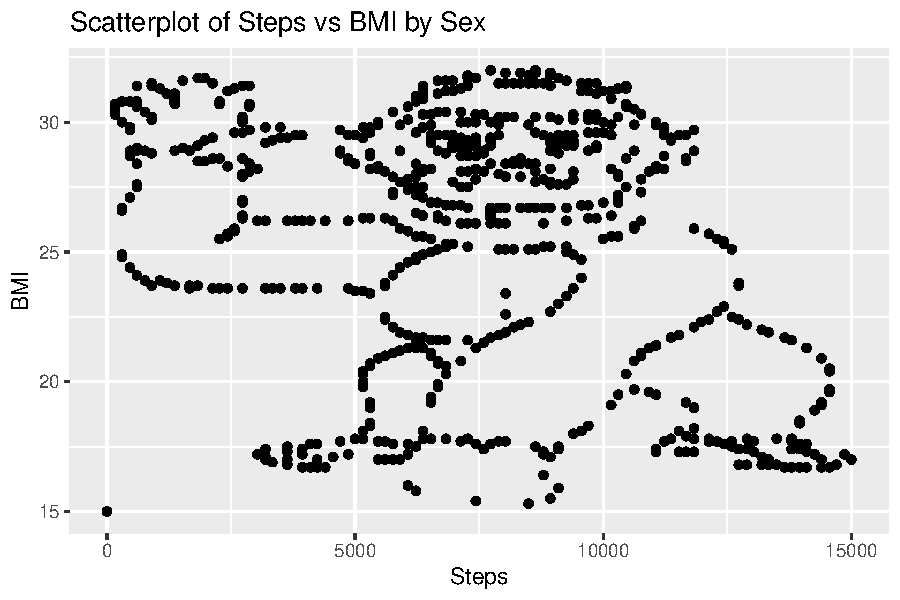
\includegraphics{_main_files/figure-latex/unnamed-chunk-18-1.pdf}

\begin{Shaded}
\begin{Highlighting}[]
\FunctionTok{ggplot}\NormalTok{(male, }\FunctionTok{aes}\NormalTok{(}\AttributeTok{x =}\NormalTok{ steps, }\AttributeTok{y =}\NormalTok{ bmi)) }\SpecialCharTok{+}
  \FunctionTok{geom\_point}\NormalTok{() }\SpecialCharTok{+}
  \FunctionTok{labs}\NormalTok{(}\AttributeTok{x =} \StringTok{"Steps"}\NormalTok{, }\AttributeTok{y =} \StringTok{"BMI"}\NormalTok{) }\SpecialCharTok{+}
  \FunctionTok{ggtitle}\NormalTok{(}\StringTok{"Scatterplot of Steps vs BMI by Sex"}\NormalTok{) }
\end{Highlighting}
\end{Shaded}

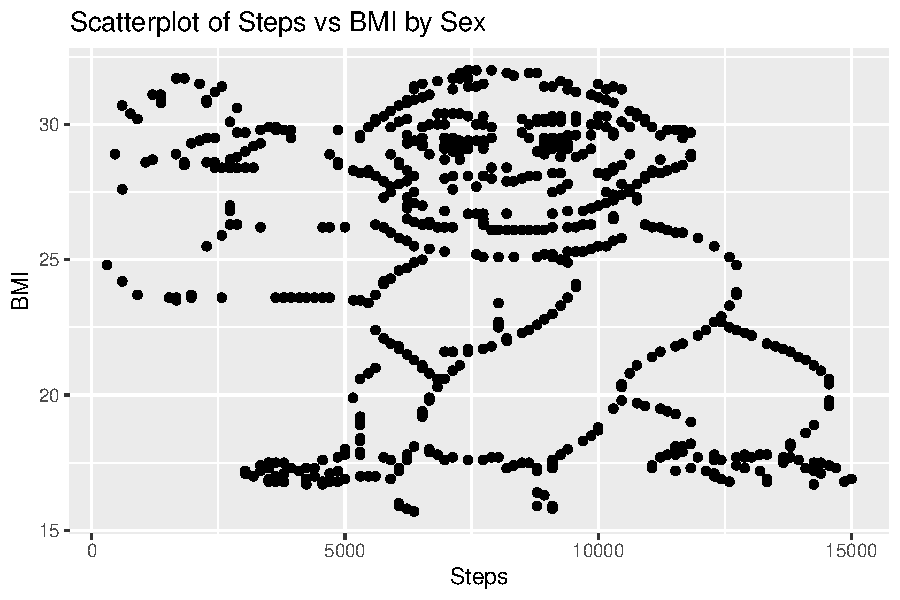
\includegraphics{_main_files/figure-latex/unnamed-chunk-18-2.pdf}

\begin{Shaded}
\begin{Highlighting}[]
\FunctionTok{ggplot}\NormalTok{(all, }\FunctionTok{aes}\NormalTok{(}\AttributeTok{x =}\NormalTok{ steps, }\AttributeTok{y =}\NormalTok{ bmi, }\AttributeTok{color =}\NormalTok{ sex)) }\SpecialCharTok{+}
  \FunctionTok{geom\_point}\NormalTok{() }\SpecialCharTok{+}
  \FunctionTok{labs}\NormalTok{(}\AttributeTok{x =} \StringTok{"Steps"}\NormalTok{, }\AttributeTok{y =} \StringTok{"BMI"}\NormalTok{) }\SpecialCharTok{+}
  \FunctionTok{ggtitle}\NormalTok{(}\StringTok{"Scatterplot of Steps vs BMI by Sex"}\NormalTok{) }\SpecialCharTok{+}
  \FunctionTok{scale\_color\_manual}\NormalTok{(}\AttributeTok{values =} \FunctionTok{c}\NormalTok{(}\StringTok{"F"} \OtherTok{=} \StringTok{"blue"}\NormalTok{, }\StringTok{"M"} \OtherTok{=} \StringTok{"red"}\NormalTok{))  }\CommentTok{\# Optional: Define color mapping}
\end{Highlighting}
\end{Shaded}

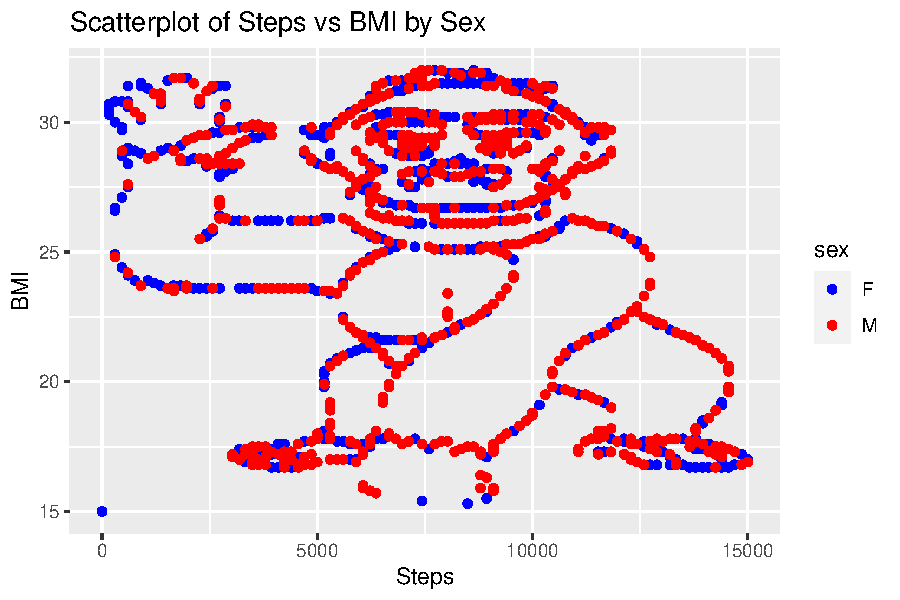
\includegraphics{_main_files/figure-latex/unnamed-chunk-18-3.pdf}

\hypertarget{solution}{%
\section{Solution}\label{solution}}

Will be made available.

\hypertarget{week-2}{%
\chapter{Week 2}\label{week-2}}

\hypertarget{exercise}{%
\section{Exercise}\label{exercise}}

\begin{itemize}
\tightlist
\item
  2nd: simulated dataset and increase the variance: how does that affects the standard error
\end{itemize}

\hypertarget{solution-1}{%
\section{Solution}\label{solution-1}}

\begin{itemize}
\item
  Data taken from \href{https://communities.sas.com/t5/Graphics-Programming/Fun-With-SAS-ODS-Graphics-Don-t-Miss-the-Gorilla-in-the-Data/td-p/697286}{here}.
\item
  Original selective attention, \href{https://www.youtube.com/watch?v=vJG698U2Mvo}{here}.
\item
  Suicide awareness campaign, \href{https://www.youtube.com/watch?v=Lw-YPKR0grk}{here}.
\end{itemize}

\hypertarget{week-3-regression-i-prediction}{%
\chapter{Week 3: Regression I (Prediction)}\label{week-3-regression-i-prediction}}

\hypertarget{aims-1}{%
\section{Aims}\label{aims-1}}

\begin{enumerate}
\def\labelenumi{\arabic{enumi}.}
\tightlist
\item
  Using regression analysis for quantitative descriptive purposes with real data
\item
  Using simulation to instantiate how different properties of the data generating process alter the reliability of regression analysis
\end{enumerate}

\hypertarget{exercise-context-and-question}{%
\section{Exercise: Context and Question}\label{exercise-context-and-question}}

As developed in the following \href{https://de.wikipedia.org/wiki/Eidgen\%C3\%B6ssische_Abstimmung_\%C3\%BCber_die_Totalrevision_des_CO2-Gesetzes\#:~:text=Die\%20Eidgen\%C3\%B6ssische\%20Abstimmung\%20\%C3\%BCber\%20die,von\%2051\%2C59\%20\%25\%20abgelehnt.}{entry}, a referendum took place in 2021 to assess whether Swiss citizens approved or not a bill aimed at reducing greenhouse gas emissions.

The bill was rejected by a narrow margin: 51.6\% of votes went for the ``No'', while 48.4\% for the ``Yes''. In the media, some analysts commented that a marked division or cleavage between rural and urban voters seems to have led to this result: a specially high rural turn-out seems to underlie such result. As the analyst commented, most urban inhabitants liked the bill while most rural inhabitants disliked it.

Not satisfied with a simple impression, as a political scientist you want to quantitatively qualify your understanding about what happened in that election. Particularly, you want to know:

\begin{enumerate}
\def\labelenumi{\arabic{enumi}.}
\tightlist
\item
  Given that more rural municipalities have smaller populations, was the turn-out higher in municipalities with smaller populations than in bigger ones?
\item
  Was the turn-out higher in more agricultural municipalities than in less agricultural ones?
\end{enumerate}

Thus, to analytically describe the voting results, you will perform some regressions using the following data.

\hypertarget{getting-the-data-first}{%
\section{Getting the data first}\label{getting-the-data-first}}

To get the data, you will use an API (application programming interface). Put plainly, for the sake of this exercise you can think of an API like a \href{https://www.youtube.com/watch?v=s7wmiS2mSXY}{waiter} to whom you make a request and who gets what ever you requested from the kitchen (a remote data source).

In this case, you will use two APIs: to get election results in Switzerland, \href{https://politanch.github.io/swissdd/index.html}{\texttt{swissdd}}, and \href{https://github.com/lgnbhl/BFS}{\texttt{BFS}} to get many other kinds of statistical information. Both APIs get information from the Federal Statistical Office (Bundesamt für Statistik).

Skimm the functions of the \href{https://politanch.github.io/swissdd/reference/index.html}{Swissdd} package. Then, inspect the \href{https://swissvotes.ch/storage/b47562b197b7725fcfa45b3e5a4abad1b4cf14cd377136f87fd4473329a51114}{codebook} to understand what for the columns and rows stand for. Do not use more than 5 minutes doing it.

To get the data, simply execute the following code. We present you with the code so, if you want, you can know how it works and you can play around with it on your own following the code's logic.

Install the \texttt{Swissdd} package

\begin{Shaded}
\begin{Highlighting}[]
\CommentTok{\#First option  {-} from CRAN. If you install it from the github repository, make sure you have the \textasciigrave{}devtools\textasciigrave{} installed in advance.}
\CommentTok{\#install.packages("swissdd")}

\CommentTok{\#Second option}
\CommentTok{\# install.packages("devtools") \# it is necessary to comment the install.packages so the book can be rendered}
\NormalTok{devtools}\SpecialCharTok{::}\FunctionTok{install\_github}\NormalTok{(}\StringTok{"politanch/swissdd"}\NormalTok{)}
\CommentTok{\# library(swissdd)}
\end{Highlighting}
\end{Shaded}

Retrieve the \href{https://swissvotes.ch/vote/644.00}{CO2 Act} information using \texttt{get\_nationalvotes}. The vote took place in 13/06/2021.

\begin{Shaded}
\begin{Highlighting}[]
\NormalTok{CO2}\OtherTok{\textless{}{-}}\FunctionTok{get\_nationalvotes}\NormalTok{(}\AttributeTok{votedates =} \StringTok{"2021{-}06{-}13"}\NormalTok{)}
\end{Highlighting}
\end{Shaded}

As the same day of the CO2 Act vote more initiatives were voted, keep only the one we care about for this exercise. Notice that each initiative has a numerical identifier called \texttt{id}. \href{https://swissvotes.ch/vote/644.00}{Here} you can find the numerical identifier under \texttt{Vote\ Nº}. Keep in mind that, the variable \texttt{id} has the same number as in \texttt{Vote\ Nº} with an additional zero to the right.

\begin{Shaded}
\begin{Highlighting}[]
\NormalTok{CO2}\OtherTok{\textless{}{-}}\NormalTok{ CO2 }\SpecialCharTok{\%\textgreater{}\%}
  \FunctionTok{filter}\NormalTok{(id}\SpecialCharTok{==}\DecValTok{6440}\NormalTok{)}
\end{Highlighting}
\end{Shaded}

The resulting data frame contains rows representing the results for a particular vote in a particular municipality. The columns qualify that vote. Use the \texttt{colnames()} function to see the names of the columns. Keep only those that might be relevant for your analysis.

\begin{Shaded}
\begin{Highlighting}[]
\NormalTok{CO2}\OtherTok{\textless{}{-}}\NormalTok{ CO2 }\SpecialCharTok{\%\textgreater{}\%}
  \FunctionTok{select}\NormalTok{(canton\_id, canton\_name, mun\_id, mun\_name, jaStimmenInProzent, jaStimmenAbsolut, neinStimmenAbsolut, stimmbeteiligungInProzent, eingelegteStimmzettel, anzahlStimmberechtigte, gueltigeStimmen)}
\end{Highlighting}
\end{Shaded}

Finally, as you want to see the turn-out differences between municipalities with different degrees of agriculture intensity you need to get some additional data. Run the following code.

\begin{Shaded}
\begin{Highlighting}[]
\CommentTok{\# install.packages("BFS")}
\CommentTok{\# library(BFS)}
\CommentTok{\#To see the information available in German}
\CommentTok{\# catalog\_data\_de \textless{}{-} bfs\_get\_catalog\_data(language = "de")}

\CommentTok{\#To see the information available in English}
\CommentTok{\#catalog\_data\_en \textless{}{-} bfs\_get\_catalog\_data(language = "en")}

\CommentTok{\#To see the information available in German that contains a particular word in the title}
\CommentTok{\#catalog\_data\_de \textless{}{-} bfs\_get\_catalog\_data(language = "de", title="Gemeinde")}

\CommentTok{\#To get the asset number (i.e., numerical id for a data set)}
\CommentTok{\# asset\_number \textless{}{-} catalog\_data\_de \%\textgreater{}\%}
\CommentTok{\#   filter(title == "Arealstatistik: Standardnomenklatur (NOAS04) nach Bezirk und Gemeinde, in Hektaren") \%\textgreater{}\%}
\CommentTok{\#   pull(number\_asset)}

\CommentTok{\#Using that asset number, the metadata (i.e., data that describes the data set) can be accessed.}
\CommentTok{\#asset\_meta \textless{}{-} bfs\_get\_asset\_metadata(number\_asset = asset\_number)}

\CommentTok{\#From the metadata, the bfs number (i.e., a alphanumeric id for the data set) can be accessed.}
\CommentTok{\#bfs\_number \textless{}{-} asset\_meta$shop$orderNr}

\CommentTok{\#Finally, using the bfs number the data set can be accessed.}
\CommentTok{\#LandUse \textless{}{-} bfs\_get\_data(number\_bfs = bfs\_number)}

\CommentTok{\#If there is a “Too Many Requests” error message, you can follow this (https://github.com/lgnbhl/BFS\#too{-}many{-}requests{-}error{-}message) }
\CommentTok{\#or download the PX file from here https://www.bfs.admin.ch/bfs/de/home/statistiken/kataloge{-}datenbanken/daten.assetdetail.24865343.html}
\CommentTok{\#install.packages("pxR")}
\CommentTok{\# library(pxR)}
\CommentTok{\#Open data}
\NormalTok{LandUse }\OtherTok{\textless{}{-}} \FunctionTok{read.px}\NormalTok{(}\StringTok{\textquotesingle{}\textasciitilde{}/Documents/0\_IPZ/2023\_2/Leemann{-}QuantMethods/QuantitativeMethods/QuantitativeMethods/Data/px{-}x{-}0202020000\_102.px\textquotesingle{}}\NormalTok{, }\AttributeTok{encoding =} \StringTok{"UTF{-}8"}\NormalTok{)}
\NormalTok{LandUseData}\OtherTok{\textless{}{-}}\NormalTok{ LandUse}\SpecialCharTok{$}\NormalTok{DATA}\SpecialCharTok{$}\NormalTok{value}

\CommentTok{\#Rename variable}
\NormalTok{LandUseData }\OtherTok{\textless{}{-}}\NormalTok{ LandUseData }\SpecialCharTok{\%\textgreater{}\%}
  \FunctionTok{rename\_with}\NormalTok{(}\SpecialCharTok{\textasciitilde{}} \StringTok{\textquotesingle{}mun\_name\textquotesingle{}}\NormalTok{, }\DecValTok{3}\NormalTok{)}

\CommentTok{\#Keep the data relevant for my analysis}
\NormalTok{LandUseData}\OtherTok{\textless{}{-}}\NormalTok{ LandUseData }\SpecialCharTok{\%\textgreater{}\%}
  \FunctionTok{filter}\NormalTok{(Periode }\SpecialCharTok{==} \StringTok{"2013/18"}\NormalTok{) }\SpecialCharTok{\%\textgreater{}\%}
  \FunctionTok{filter}\NormalTok{(Standardnomenklatur..NOAS04.}\SpecialCharTok{==}\StringTok{"{-}b Landwirtschaftsflächen"} \SpecialCharTok{|}\NormalTok{ Standardnomenklatur..NOAS04.}\SpecialCharTok{==}\StringTok{"Fläche Total"}\NormalTok{) }\SpecialCharTok{\%\textgreater{}\%}
  \FunctionTok{filter}\NormalTok{(}\FunctionTok{str\_starts}\NormalTok{(}\FunctionTok{str\_trim}\NormalTok{(mun\_name), }\FunctionTok{fixed}\NormalTok{(}\StringTok{"."}\NormalTok{))) }\SpecialCharTok{\%\textgreater{}\%}
  \FunctionTok{mutate}\NormalTok{(}\AttributeTok{mun\_name =} \FunctionTok{str\_replace\_all}\NormalTok{(mun\_name, }\FunctionTok{fixed}\NormalTok{(}\StringTok{"......"}\NormalTok{), }\StringTok{""}\NormalTok{))}

\CommentTok{\# install.packages("tidyverse")}
\CommentTok{\#Adjust data from long to wide}
\NormalTok{LandUseData }\OtherTok{\textless{}{-}}\NormalTok{ LandUseData }\SpecialCharTok{\%\textgreater{}\%}
  \FunctionTok{pivot\_wider}\NormalTok{(}\AttributeTok{names\_from =}\NormalTok{ Standardnomenklatur..NOAS04., }\AttributeTok{values\_from =}\NormalTok{ value)}

\CommentTok{\#Rename variables}
\NormalTok{LandUseData }\OtherTok{\textless{}{-}}\NormalTok{ LandUseData }\SpecialCharTok{\%\textgreater{}\%}
  \FunctionTok{rename\_with}\NormalTok{(}\SpecialCharTok{\textasciitilde{}} \StringTok{\textquotesingle{}TotalAreaHa\textquotesingle{}}\NormalTok{, }\DecValTok{3}\NormalTok{) }\SpecialCharTok{\%\textgreater{}\%}
  \FunctionTok{rename\_with}\NormalTok{(}\SpecialCharTok{\textasciitilde{}} \StringTok{\textquotesingle{}AgriculturalAreaHa\textquotesingle{}}\NormalTok{, }\DecValTok{4}\NormalTok{) }\SpecialCharTok{\%\textgreater{}\%}
  \FunctionTok{select}\NormalTok{(}\SpecialCharTok{{-}}\NormalTok{Periode)}
\end{Highlighting}
\end{Shaded}

Using the additional data, you can now merge both data sets so you can know how did voters behave in more agricultural areas. Use the \texttt{inner\_join} function. The numerical IDs are available in \texttt{LandUseData} but not in \texttt{CO2}. However, as both sources share the \texttt{mun\_name}, you use that variable to match them.

\begin{Shaded}
\begin{Highlighting}[]
\NormalTok{CO2 }\OtherTok{\textless{}{-}} \FunctionTok{inner\_join}\NormalTok{(CO2, LandUseData, }\AttributeTok{by=}\StringTok{"mun\_name"}\NormalTok{)  }
\end{Highlighting}
\end{Shaded}

\hypertarget{exercise-solution}{%
\section{Exercise: solution}\label{exercise-solution}}

\textbf{Note:} Remember that you can copy the code from one point to answer another point. Simply make the necessary adjustments.

\hypertarget{real-data}{%
\subsection{Real data}\label{real-data}}

Using the previous data, you do the following to answer your two questions:

\begin{enumerate}
\def\labelenumi{\roman{enumi}.}
\tightlist
\item
  Since you want to describe the turn-out across municipalities with different population sizes, you initially think of regressing the turn-out on the population size. As you lack the municipal population, you use the number of eligible voters \texttt{anzahlStimmberechtigte} as a proxy. Regress \texttt{stimmbeteiligungInProzent} (Voting participation in percent) on \texttt{anzahlStimmberechtigte} (number of eligible voters) \href{https://www.geeksforgeeks.org/remove-intercept-from-regression-model-in-r/}{without} the intercept. Report and interpret the parameter.
\end{enumerate}

Write the regression here.

\begin{Shaded}
\begin{Highlighting}[]
\NormalTok{result }\OtherTok{\textless{}{-}} \FunctionTok{lm}\NormalTok{(stimmbeteiligungInProzent }\SpecialCharTok{\textasciitilde{}}\NormalTok{ anzahlStimmberechtigte }\SpecialCharTok{{-}}\DecValTok{1}\NormalTok{ , }\AttributeTok{data =}\NormalTok{ CO2)}
\FunctionTok{summary}\NormalTok{(result)}
\end{Highlighting}
\end{Shaded}

\begin{verbatim}
## 
## Call:
## lm(formula = stimmbeteiligungInProzent ~ anzahlStimmberechtigte - 
##     1, data = CO2)
## 
## Residuals:
##     Min      1Q  Median      3Q     Max 
## -556.58   52.77   61.07   68.11   96.02 
## 
## Coefficients:
##                         Estimate Std. Error t value Pr(>|t|)    
## anzahlStimmberechtigte 0.0026344  0.0001777   14.82   <2e-16 ***
## ---
## Signif. codes:  0 '***' 0.001 '**' 0.01 '*' 0.05 '.' 0.1 ' ' 1
## 
## Residual standard error: 62.41 on 2131 degrees of freedom
## Multiple R-squared:  0.09349,    Adjusted R-squared:  0.09307 
## F-statistic: 219.8 on 1 and 2131 DF,  p-value: < 2.2e-16
\end{verbatim}

Report and interpret the parameter here.

\begin{Shaded}
\begin{Highlighting}[]
\NormalTok{coeffs}\OtherTok{\textless{}{-}} \FunctionTok{coef}\NormalTok{(result)}

\FunctionTok{cat}\NormalTok{(}\StringTok{\textquotesingle{}The beta value for\textquotesingle{}}\NormalTok{, }\FunctionTok{names}\NormalTok{(coeffs[}\DecValTok{1}\NormalTok{]), }\StringTok{\textquotesingle{} is \textquotesingle{}}\NormalTok{, }\FunctionTok{round}\NormalTok{(}\FunctionTok{unname}\NormalTok{(coeffs[}\DecValTok{1}\NormalTok{]), }\AttributeTok{digits =} \DecValTok{5}\NormalTok{), }\StringTok{\textquotesingle{}. It means that, across Swiss municipalities an increase of a thousand voters was associated with an average increase in the turn{-}out of \textquotesingle{}}\NormalTok{, }\FunctionTok{round}\NormalTok{(}\FunctionTok{unname}\NormalTok{(coeffs[}\DecValTok{1}\NormalTok{])}\SpecialCharTok{*}\DecValTok{1000}\NormalTok{, }\AttributeTok{digits =} \DecValTok{5}\NormalTok{), }\StringTok{\textquotesingle{} percentage points.\textquotesingle{}}\NormalTok{)}
\end{Highlighting}
\end{Shaded}

\begin{verbatim}
## The beta value for anzahlStimmberechtigte  is  0.00263 . It means that, across Swiss municipalities an increase of a thousand voters was associated with an average increase in the turn-out of  2.63439  percentage points.
\end{verbatim}

\begin{enumerate}
\def\labelenumi{\roman{enumi}.}
\item
  {[}Optional{]} Why could the number of eligible voters inform better your inquiry than the total municipal population? What difference across municipalities could make an analysis based on municipal population render the analysis less reliable?
\item
  To enrich your analysis, you generate a scatter plot showing the relation between the same pair of variables and qualifying it adding the regression line. Remember that you are doing the analysis without the intercept.
\end{enumerate}

\begin{Shaded}
\begin{Highlighting}[]
\CommentTok{\# Create a scatter plot}
\FunctionTok{ggplot}\NormalTok{(CO2, }\FunctionTok{aes}\NormalTok{(}\AttributeTok{x =}\NormalTok{ anzahlStimmberechtigte, }\AttributeTok{y =}\NormalTok{ stimmbeteiligungInProzent)) }\SpecialCharTok{+}
  \FunctionTok{geom\_point}\NormalTok{() }\SpecialCharTok{+}
  \FunctionTok{geom\_smooth}\NormalTok{(}\AttributeTok{method =} \StringTok{"lm"}\NormalTok{, }\AttributeTok{formula =}\NormalTok{ y }\SpecialCharTok{\textasciitilde{}}\NormalTok{ x }\SpecialCharTok{{-}} \DecValTok{1}\NormalTok{, }\AttributeTok{se =} \ConstantTok{FALSE}\NormalTok{, }\AttributeTok{color =} \StringTok{"purple"}\NormalTok{) }\SpecialCharTok{+}  \CommentTok{\# Adding the regression line}
  \FunctionTok{scale\_y\_continuous}\NormalTok{(}\AttributeTok{limits =} \FunctionTok{c}\NormalTok{(}\DecValTok{0}\NormalTok{, }\FunctionTok{max}\NormalTok{(CO2}\SpecialCharTok{$}\NormalTok{stimmbeteiligungInProzent, }\AttributeTok{na.rm =} \ConstantTok{TRUE}\NormalTok{))) }\SpecialCharTok{+}  
  \FunctionTok{theme\_minimal}\NormalTok{() }\SpecialCharTok{+}
  \FunctionTok{labs}\NormalTok{(}
    \AttributeTok{x =} \StringTok{"Number of eligible voters"}\NormalTok{,}
    \AttributeTok{y =} \StringTok{"Voting Participation (\%)"}\NormalTok{,}
    \AttributeTok{title =} \StringTok{"Scatter plot with Linear Regression Line"}
\NormalTok{  )}
\end{Highlighting}
\end{Shaded}

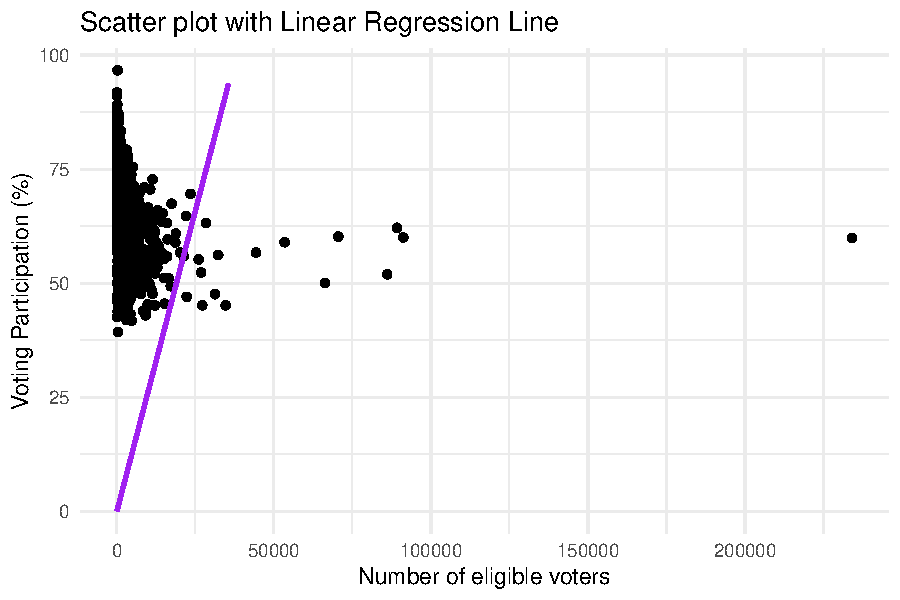
\includegraphics{_main_files/figure-latex/unnamed-chunk-29-1.pdf}

\begin{enumerate}
\def\labelenumi{\roman{enumi}.}
\tightlist
\item
  Given your preliminary analysis, you find that, on average, municipalities with bigger populations had a higher turn-out than those with smaller ones. As you know that most urban citizens preferred `Yes' but the `No' won, you call into question your first approach: while bigger municipalities had higher participation levels than smaller ones, the option preferred by most rural inhabitants won. In other words, it is not clear that the population size helps us to understand this voting results.
\end{enumerate}

Thus, to capture how rural a municipality is, you used the agricultural area of the municipality (\texttt{AgriculturalAreaHa}) as a regressor (aka. independent variable) for the same regressand (aka. dependent variable) of the previous point (i.e., voting participation in percent). Again, do the regression without intercept. Report and interpret the parameter. Also present the corresponding graph.

Write the regression here.

\begin{Shaded}
\begin{Highlighting}[]
\NormalTok{result }\OtherTok{\textless{}{-}} \FunctionTok{lm}\NormalTok{(stimmbeteiligungInProzent }\SpecialCharTok{\textasciitilde{}}\NormalTok{ AgriculturalAreaHa }\SpecialCharTok{{-}}\DecValTok{1}\NormalTok{ , }\AttributeTok{data =}\NormalTok{ CO2)}
\FunctionTok{summary}\NormalTok{(result)}
\end{Highlighting}
\end{Shaded}

\begin{verbatim}
## 
## Call:
## lm(formula = stimmbeteiligungInProzent ~ AgriculturalAreaHa - 
##     1, data = CO2)
## 
## Residuals:
##     Min      1Q  Median      3Q     Max 
## -357.41   40.38   51.27   58.59   87.83 
## 
## Coefficients:
##                     Estimate Std. Error t value Pr(>|t|)    
## AgriculturalAreaHa 0.0312861  0.0009688   32.29   <2e-16 ***
## ---
## Signif. codes:  0 '***' 0.001 '**' 0.01 '*' 0.05 '.' 0.1 ' ' 1
## 
## Residual standard error: 53.71 on 2131 degrees of freedom
## Multiple R-squared:  0.3286, Adjusted R-squared:  0.3283 
## F-statistic:  1043 on 1 and 2131 DF,  p-value: < 2.2e-16
\end{verbatim}

Report and interpret the parameter here.

\begin{Shaded}
\begin{Highlighting}[]
\NormalTok{coeffs}\OtherTok{\textless{}{-}} \FunctionTok{coef}\NormalTok{(result)}
\FunctionTok{cat}\NormalTok{(}\StringTok{\textquotesingle{}The beta value for\textquotesingle{}}\NormalTok{, }\FunctionTok{names}\NormalTok{(coeffs[}\DecValTok{1}\NormalTok{]), }\StringTok{\textquotesingle{} is \textquotesingle{}}\NormalTok{, }\FunctionTok{round}\NormalTok{(}\FunctionTok{unname}\NormalTok{(coeffs[}\DecValTok{1}\NormalTok{]), }\AttributeTok{digits =} \DecValTok{5}\NormalTok{), }\StringTok{\textquotesingle{}. It means that, across Swiss municipalities an increase of a thousand hectares was associated with an average increase in the turn{-}out of \textquotesingle{}}\NormalTok{, }\FunctionTok{round}\NormalTok{(}\FunctionTok{unname}\NormalTok{(coeffs[}\DecValTok{1}\NormalTok{])}\SpecialCharTok{*}\DecValTok{1000}\NormalTok{, }\AttributeTok{digits =} \DecValTok{5}\NormalTok{), }\StringTok{\textquotesingle{} percentage points.\textquotesingle{}}\NormalTok{)}
\end{Highlighting}
\end{Shaded}

\begin{verbatim}
## The beta value for AgriculturalAreaHa  is  0.03129 . It means that, across Swiss municipalities an increase of a thousand hectares was associated with an average increase in the turn-out of  31.28612  percentage points.
\end{verbatim}

Present the graph here.

\begin{Shaded}
\begin{Highlighting}[]
\CommentTok{\# Create a scatter plot}
\FunctionTok{ggplot}\NormalTok{(CO2, }\FunctionTok{aes}\NormalTok{(}\AttributeTok{x =}\NormalTok{ AgriculturalAreaHa, }\AttributeTok{y =}\NormalTok{ stimmbeteiligungInProzent)) }\SpecialCharTok{+}
  \FunctionTok{geom\_point}\NormalTok{() }\SpecialCharTok{+}
  \FunctionTok{geom\_smooth}\NormalTok{(}\AttributeTok{method =} \StringTok{"lm"}\NormalTok{, }\AttributeTok{formula =}\NormalTok{ y }\SpecialCharTok{\textasciitilde{}}\NormalTok{ x }\SpecialCharTok{{-}} \DecValTok{1}\NormalTok{, }\AttributeTok{se =} \ConstantTok{FALSE}\NormalTok{, }\AttributeTok{color =} \StringTok{"purple"}\NormalTok{) }\SpecialCharTok{+}  \CommentTok{\# Adding the regression line}
  \FunctionTok{scale\_y\_continuous}\NormalTok{(}\AttributeTok{limits =} \FunctionTok{c}\NormalTok{(}\DecValTok{0}\NormalTok{, }\FunctionTok{max}\NormalTok{(CO2}\SpecialCharTok{$}\NormalTok{stimmbeteiligungInProzent, }\AttributeTok{na.rm =} \ConstantTok{TRUE}\NormalTok{))) }\SpecialCharTok{+}  \CommentTok{\#}
  \FunctionTok{theme\_minimal}\NormalTok{() }\SpecialCharTok{+}
  \FunctionTok{labs}\NormalTok{(}
    \AttributeTok{x =} \StringTok{"Agricultural Area (Ha)"}\NormalTok{,}
    \AttributeTok{y =} \StringTok{"Voting Participation (\%)"}\NormalTok{,}
    \AttributeTok{title =} \StringTok{"Scatter plot with Linear Regression Line"}
\NormalTok{  )}
\end{Highlighting}
\end{Shaded}

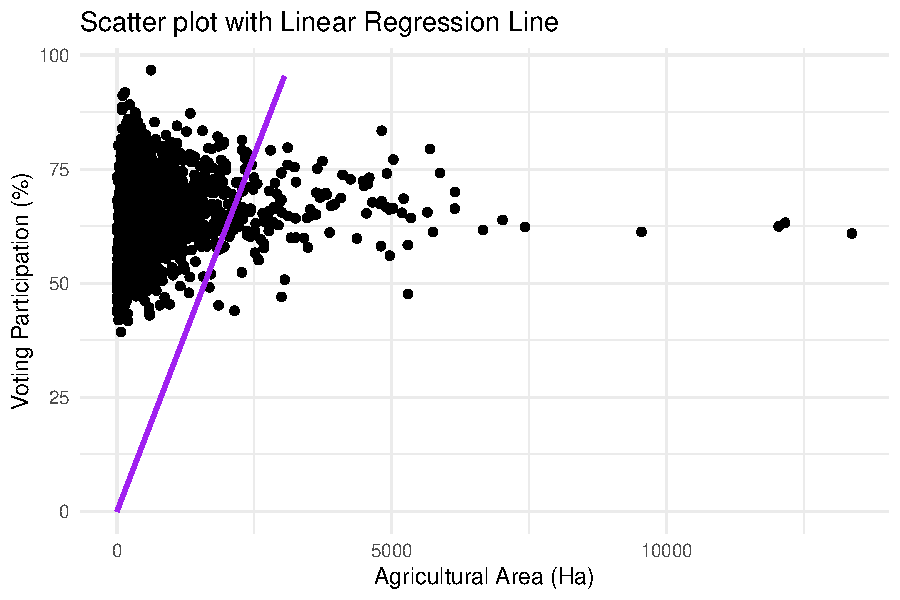
\includegraphics{_main_files/figure-latex/unnamed-chunk-32-1.pdf}

\begin{enumerate}
\def\labelenumi{\roman{enumi}.}
\tightlist
\item
  The result from the previous point is consistent with the vote result given the urban-rural divide in preferences (i.e., municipalities with more agricultural area had higher participation rates). However, you notice that your comparisons across municipalities are not very rigorous because you are ignoring how important agricultural land with respect to the whole municipality area. An implication of that is that two municipalities with the same agricultural area could be taken as equally rural while one could have a very big urban area (e.g., Zurich) and the other have a very small one.
\end{enumerate}

Thus to make your analysis across more comparable units, you transform the absolute value of the agricultural area to a relative one: the percentage of the municipal area that is agricultural. Create the variable \texttt{AgricAreaPercent} to represent those transformed values. Regress the turn-out on the newly created variable. Again, do the regression without intercept. Report and interpret the parameter. Also present the corresponding graph.

Write the regression here.

\begin{Shaded}
\begin{Highlighting}[]
\CommentTok{\#Transform the units to make them comparable }
\NormalTok{CO2 }\OtherTok{\textless{}{-}}\NormalTok{ CO2 }\SpecialCharTok{\%\textgreater{}\%}
  \FunctionTok{mutate}\NormalTok{(}\AttributeTok{AgricAreaPercent=} \DecValTok{100}\SpecialCharTok{*}\NormalTok{AgriculturalAreaHa}\SpecialCharTok{/}\NormalTok{TotalAreaHa)}

\CommentTok{\#regression}
\NormalTok{result0 }\OtherTok{\textless{}{-}} \FunctionTok{lm}\NormalTok{(stimmbeteiligungInProzent }\SpecialCharTok{\textasciitilde{}}\NormalTok{ AgricAreaPercent }\SpecialCharTok{{-}}\DecValTok{1}\NormalTok{ , }\AttributeTok{data =}\NormalTok{ CO2)}
\FunctionTok{summary}\NormalTok{(result0)}
\end{Highlighting}
\end{Shaded}

\begin{verbatim}
## 
## Call:
## lm(formula = stimmbeteiligungInProzent ~ AgricAreaPercent - 1, 
##     data = CO2)
## 
## Residuals:
##     Min      1Q  Median      3Q     Max 
## -42.102  -7.509   6.449  23.631  83.331 
## 
## Coefficients:
##                  Estimate Std. Error t value Pr(>|t|)    
## AgricAreaPercent  1.26144    0.01012   124.7   <2e-16 ***
## ---
## Signif. codes:  0 '***' 0.001 '**' 0.01 '*' 0.05 '.' 0.1 ' ' 1
## 
## Residual standard error: 22.75 on 2131 degrees of freedom
## Multiple R-squared:  0.8795, Adjusted R-squared:  0.8794 
## F-statistic: 1.555e+04 on 1 and 2131 DF,  p-value: < 2.2e-16
\end{verbatim}

Report and interpret the parameter here.

\begin{Shaded}
\begin{Highlighting}[]
\NormalTok{coeffs}\OtherTok{\textless{}{-}} \FunctionTok{coef}\NormalTok{(result0)}
\FunctionTok{cat}\NormalTok{(}\StringTok{\textquotesingle{}The beta value for\textquotesingle{}}\NormalTok{, }\FunctionTok{names}\NormalTok{(coeffs[}\DecValTok{1}\NormalTok{]), }\StringTok{\textquotesingle{} is \textquotesingle{}}\NormalTok{, }\FunctionTok{round}\NormalTok{(}\FunctionTok{unname}\NormalTok{(coeffs[}\DecValTok{1}\NormalTok{]), }\AttributeTok{digits =} \DecValTok{2}\NormalTok{), }\StringTok{\textquotesingle{}. It means that, across Swiss municipalities an increase of one percentage point in the share of agricultural land was associated with an average increase in the turn{-}out of \textquotesingle{}}\NormalTok{, }\FunctionTok{round}\NormalTok{(}\FunctionTok{unname}\NormalTok{(coeffs[}\DecValTok{1}\NormalTok{]), }\AttributeTok{digits =} \DecValTok{2}\NormalTok{), }\StringTok{\textquotesingle{} percentage points.\textquotesingle{}}\NormalTok{)}
\end{Highlighting}
\end{Shaded}

\begin{verbatim}
## The beta value for AgricAreaPercent  is  1.26 . It means that, across Swiss municipalities an increase of one percentage point in the share of agricultural land was associated with an average increase in the turn-out of  1.26  percentage points.
\end{verbatim}

Present the graph here.

\begin{Shaded}
\begin{Highlighting}[]
\CommentTok{\# Create a scatter plot}
\FunctionTok{ggplot}\NormalTok{(CO2, }\FunctionTok{aes}\NormalTok{(}\AttributeTok{x =}\NormalTok{ AgricAreaPercent, }\AttributeTok{y =}\NormalTok{ stimmbeteiligungInProzent)) }\SpecialCharTok{+}
  \FunctionTok{geom\_point}\NormalTok{() }\SpecialCharTok{+}
  \FunctionTok{geom\_smooth}\NormalTok{(}\AttributeTok{method =} \StringTok{"lm"}\NormalTok{, }\AttributeTok{formula =}\NormalTok{ y }\SpecialCharTok{\textasciitilde{}}\NormalTok{ x }\SpecialCharTok{{-}} \DecValTok{1}\NormalTok{, }\AttributeTok{se =} \ConstantTok{FALSE}\NormalTok{, }\AttributeTok{color =} \StringTok{"purple"}\NormalTok{) }\SpecialCharTok{+}  \CommentTok{\# Adding the regression line}
  \FunctionTok{scale\_y\_continuous}\NormalTok{(}\AttributeTok{limits =} \FunctionTok{c}\NormalTok{(}\DecValTok{0}\NormalTok{, }\FunctionTok{max}\NormalTok{(CO2}\SpecialCharTok{$}\NormalTok{stimmbeteiligungInProzent, }\AttributeTok{na.rm =} \ConstantTok{TRUE}\NormalTok{))) }\SpecialCharTok{+}  \CommentTok{\#}
  \FunctionTok{theme\_minimal}\NormalTok{() }\SpecialCharTok{+}
  \FunctionTok{labs}\NormalTok{(}
    \AttributeTok{x =} \StringTok{"Agricultural Area (\%)"}\NormalTok{,}
    \AttributeTok{y =} \StringTok{"Voting Participation (\%)"}\NormalTok{,}
    \AttributeTok{title =} \StringTok{"Scatter plot with Linear Regression Line"}
\NormalTok{  )}
\end{Highlighting}
\end{Shaded}

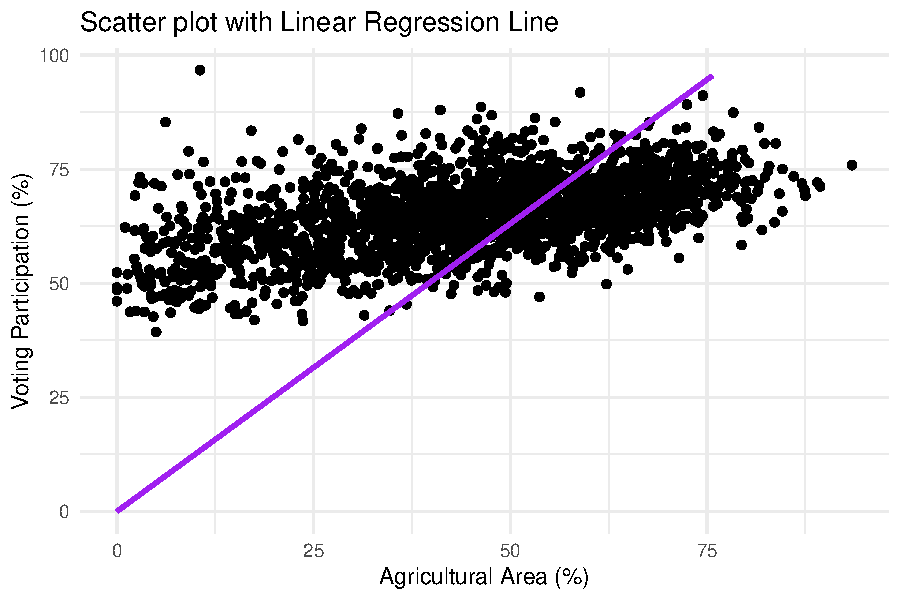
\includegraphics{_main_files/figure-latex/unnamed-chunk-35-1.pdf}

\begin{enumerate}
\def\labelenumi{\roman{enumi}.}
\tightlist
\item
  The previous graph showed you the same relationship consistent with the vote. However, you now notice that the regression line is strange: if it is supposed to be the line described the general tendency in the relation between two variables, it is strange that it is very far from many observations and only close to few of them. Hence, you remember that the using the intercept increases the fit of the line. Accordingly, you do all the same steps of the previous point but this time with the intercept.
\end{enumerate}

Write the regression here.

\begin{Shaded}
\begin{Highlighting}[]
\CommentTok{\#regression}
\NormalTok{result1 }\OtherTok{\textless{}{-}} \FunctionTok{lm}\NormalTok{(stimmbeteiligungInProzent }\SpecialCharTok{\textasciitilde{}}\NormalTok{ AgricAreaPercent, }\AttributeTok{data =}\NormalTok{ CO2)}
\FunctionTok{summary}\NormalTok{(result1)}
\end{Highlighting}
\end{Shaded}

\begin{verbatim}
## 
## Call:
## lm(formula = stimmbeteiligungInProzent ~ AgricAreaPercent, data = CO2)
## 
## Residuals:
##     Min      1Q  Median      3Q     Max 
## -19.971  -4.760  -0.270   4.314  39.145 
## 
## Coefficients:
##                   Estimate Std. Error t value Pr(>|t|)    
## (Intercept)      55.189867   0.384603   143.5   <2e-16 ***
## AgricAreaPercent  0.219491   0.007894    27.8   <2e-16 ***
## ---
## Signif. codes:  0 '***' 0.001 '**' 0.01 '*' 0.05 '.' 0.1 ' ' 1
## 
## Residual standard error: 6.969 on 2130 degrees of freedom
## Multiple R-squared:  0.2663, Adjusted R-squared:  0.2659 
## F-statistic: 773.1 on 1 and 2130 DF,  p-value: < 2.2e-16
\end{verbatim}

Report and interpret the parameter here.

\begin{Shaded}
\begin{Highlighting}[]
\NormalTok{coeffs}\OtherTok{\textless{}{-}} \FunctionTok{coef}\NormalTok{(result1)}
\FunctionTok{cat}\NormalTok{(}\StringTok{\textquotesingle{}The beta value for\textquotesingle{}}\NormalTok{, }\FunctionTok{names}\NormalTok{(coeffs[}\DecValTok{2}\NormalTok{]), }\StringTok{\textquotesingle{} is \textquotesingle{}}\NormalTok{, }\FunctionTok{round}\NormalTok{(}\FunctionTok{unname}\NormalTok{(coeffs[}\DecValTok{2}\NormalTok{]), }\AttributeTok{digits =} \DecValTok{2}\NormalTok{), }\StringTok{\textquotesingle{}. It means that, across Swiss municipalities an increase of one percentage point in the share of agricultural land was associated with an average increase in the turn{-}out of \textquotesingle{}}\NormalTok{, }\FunctionTok{round}\NormalTok{(}\FunctionTok{unname}\NormalTok{(coeffs[}\DecValTok{2}\NormalTok{]), }\AttributeTok{digits =} \DecValTok{2}\NormalTok{), }\StringTok{\textquotesingle{} percentage points.}\SpecialCharTok{\textbackslash{}n\textbackslash{}n}\StringTok{Likewise, should there be a municipality with no agricultural area, we could expect it to have a turn{-}out of \textquotesingle{}}\NormalTok{, }\FunctionTok{round}\NormalTok{(}\FunctionTok{unname}\NormalTok{(coeffs[}\DecValTok{1}\NormalTok{]), }\AttributeTok{digits =} \DecValTok{2}\NormalTok{), }\StringTok{\textquotesingle{}. From there on, increasing one percentage point at a time up to 100 percentage points (i.e., a municipality with 100\% of agricultural area), we would have a turn{-}out of \textquotesingle{}}\NormalTok{, }\FunctionTok{round}\NormalTok{(}\FunctionTok{unname}\NormalTok{(coeffs[}\DecValTok{1}\NormalTok{]), }\AttributeTok{digits =} \DecValTok{2}\NormalTok{)}\SpecialCharTok{+}\FunctionTok{round}\NormalTok{(}\FunctionTok{unname}\NormalTok{(coeffs[}\DecValTok{2}\NormalTok{]}\SpecialCharTok{*}\DecValTok{100}\NormalTok{), }\AttributeTok{digits =} \DecValTok{2}\NormalTok{))}
\end{Highlighting}
\end{Shaded}

\begin{verbatim}
## The beta value for AgricAreaPercent  is  0.22 . It means that, across Swiss municipalities an increase of one percentage point in the share of agricultural land was associated with an average increase in the turn-out of  0.22  percentage points.
## 
## Likewise, should there be a municipality with no agricultural area, we could expect it to have a turn-out of  55.19 . From there on, increasing one percentage point at a time up to 100 percentage points (i.e., a municipality with 100% of agricultural area), we would have a turn-out of  77.14
\end{verbatim}

Present the graph here.

\begin{Shaded}
\begin{Highlighting}[]
\CommentTok{\# Create a scatter plot}
\FunctionTok{ggplot}\NormalTok{(CO2, }\FunctionTok{aes}\NormalTok{(}\AttributeTok{x =}\NormalTok{ AgricAreaPercent, }\AttributeTok{y =}\NormalTok{ stimmbeteiligungInProzent)) }\SpecialCharTok{+}
  \FunctionTok{geom\_point}\NormalTok{() }\SpecialCharTok{+}
  \FunctionTok{geom\_smooth}\NormalTok{(}\AttributeTok{method =} \StringTok{"lm"}\NormalTok{, }\AttributeTok{formula =}\NormalTok{ y }\SpecialCharTok{\textasciitilde{}}\NormalTok{ x, }\AttributeTok{se =} \ConstantTok{FALSE}\NormalTok{, }\AttributeTok{color =} \StringTok{"purple"}\NormalTok{) }\SpecialCharTok{+}  \CommentTok{\# Adding the regression line}
  \FunctionTok{scale\_y\_continuous}\NormalTok{(}\AttributeTok{limits =} \FunctionTok{c}\NormalTok{(}\DecValTok{25}\NormalTok{, }\FunctionTok{max}\NormalTok{(CO2}\SpecialCharTok{$}\NormalTok{stimmbeteiligungInProzent, }\AttributeTok{na.rm =} \ConstantTok{TRUE}\NormalTok{))) }\SpecialCharTok{+}  \CommentTok{\#}
  \FunctionTok{theme\_minimal}\NormalTok{() }\SpecialCharTok{+}
  \FunctionTok{labs}\NormalTok{(}
    \AttributeTok{x =} \StringTok{"Agricultural Area (\%)"}\NormalTok{,}
    \AttributeTok{y =} \StringTok{"Voting Participation (\%)"}\NormalTok{,}
    \AttributeTok{title =} \StringTok{"Scatter plot with Linear Regression Line"}
\NormalTok{  )}
\end{Highlighting}
\end{Shaded}

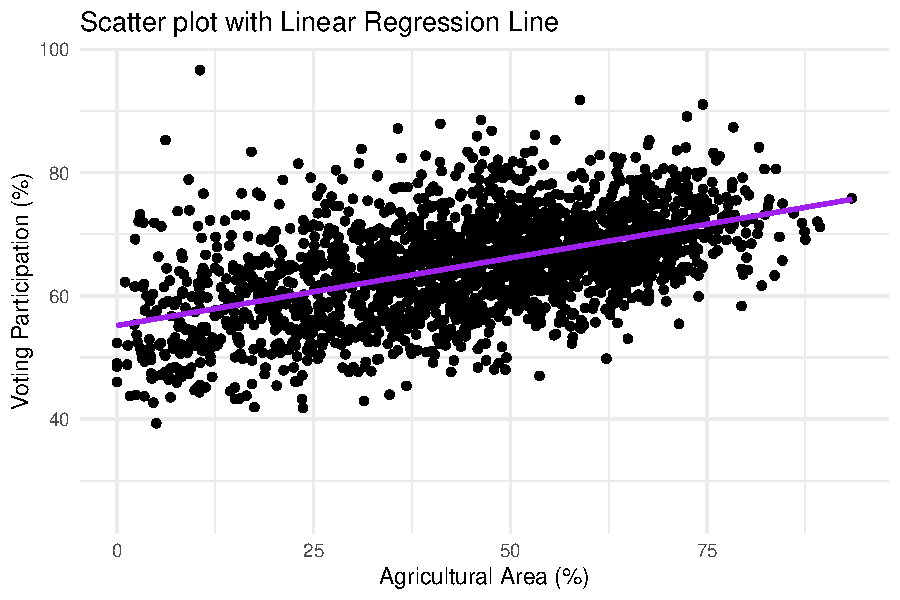
\includegraphics{_main_files/figure-latex/unnamed-chunk-38-1.pdf}

\begin{enumerate}
\def\labelenumi{\roman{enumi}.}
\tightlist
\item
  {[}Optional{]} You noticed that the regression using the intercept fits better the data: on average, the distance from each point to the regression line is lower. See this \href{https://en.wikipedia.org/wiki/Coefficient_of_determination}{entry}, particularly the graph with the blue and red squares to understand the logic of the R\^{}2 as a measure for goodness of fit. You want to compare both the regression lines with and without the intercept in one same graph. Do it. What lesson can you get from this comparison?
\end{enumerate}

\begin{Shaded}
\begin{Highlighting}[]
\FunctionTok{ggplot}\NormalTok{(CO2, }\FunctionTok{aes}\NormalTok{(}\AttributeTok{x =}\NormalTok{ AgricAreaPercent, }\AttributeTok{y =}\NormalTok{ stimmbeteiligungInProzent)) }\SpecialCharTok{+}
  \FunctionTok{geom\_point}\NormalTok{() }\SpecialCharTok{+}
  \FunctionTok{geom\_smooth}\NormalTok{(}\AttributeTok{method =} \StringTok{"lm"}\NormalTok{, }\AttributeTok{formula =}\NormalTok{ y }\SpecialCharTok{\textasciitilde{}}\NormalTok{ x}\DecValTok{{-}1}\NormalTok{, }\AttributeTok{se =} \ConstantTok{FALSE}\NormalTok{, }\AttributeTok{color =} \StringTok{"red"}\NormalTok{) }\SpecialCharTok{+}  \CommentTok{\# Adding the regression line}
  \FunctionTok{geom\_smooth}\NormalTok{(}\AttributeTok{method =} \StringTok{"lm"}\NormalTok{, }\AttributeTok{formula =}\NormalTok{ y }\SpecialCharTok{\textasciitilde{}}\NormalTok{ x, }\AttributeTok{se =} \ConstantTok{FALSE}\NormalTok{, }\AttributeTok{color =} \StringTok{"purple"}\NormalTok{) }\SpecialCharTok{+}  \CommentTok{\# Adding the regression line}
  \FunctionTok{scale\_y\_continuous}\NormalTok{(}\AttributeTok{limits =} \FunctionTok{c}\NormalTok{(}\DecValTok{25}\NormalTok{, }\FunctionTok{max}\NormalTok{(CO2}\SpecialCharTok{$}\NormalTok{stimmbeteiligungInProzent, }\AttributeTok{na.rm =} \ConstantTok{TRUE}\NormalTok{))) }\SpecialCharTok{+}  \CommentTok{\#}
  \FunctionTok{theme\_minimal}\NormalTok{() }\SpecialCharTok{+}
  \FunctionTok{labs}\NormalTok{(}
    \AttributeTok{x =} \StringTok{"Agricultural Area (\%)"}\NormalTok{,}
    \AttributeTok{y =} \StringTok{"Voting Participation (\%)"}\NormalTok{,}
    \AttributeTok{title =} \StringTok{"Scatter plot with Linear Regression Line"}
\NormalTok{  )}
\end{Highlighting}
\end{Shaded}

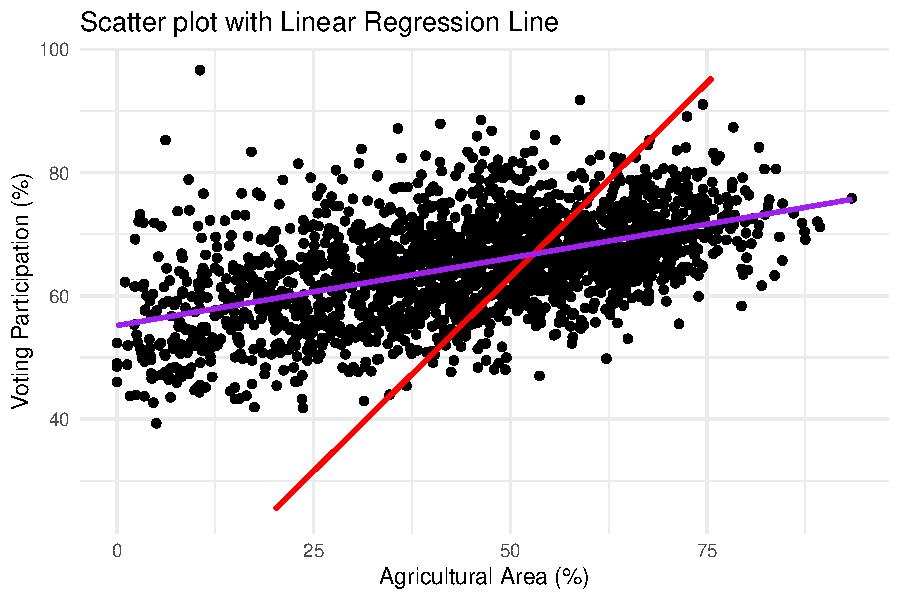
\includegraphics{_main_files/figure-latex/unnamed-chunk-39-1.pdf}

\begin{enumerate}
\def\labelenumi{\roman{enumi}.}
\tightlist
\item
  {[}Optional{]} Now add a vertical line with the average for the agricultural area, and a horizontal one with the average turn-out. What does this new graph tell you about the descriptive performance of a regression with and without intercepts?
\end{enumerate}

\begin{Shaded}
\begin{Highlighting}[]
\CommentTok{\#Means for Y and X}
\NormalTok{mean\_AgricAreaPercent }\OtherTok{\textless{}{-}} \FunctionTok{mean}\NormalTok{(CO2}\SpecialCharTok{$}\NormalTok{AgricAreaPercent, }\AttributeTok{na.rm =} \ConstantTok{TRUE}\NormalTok{)}
\NormalTok{mean\_stimmbeteiligungInProzent }\OtherTok{\textless{}{-}} \FunctionTok{mean}\NormalTok{(CO2}\SpecialCharTok{$}\NormalTok{stimmbeteiligungInProzent, }\AttributeTok{na.rm =} \ConstantTok{TRUE}\NormalTok{)}

\CommentTok{\# Create a scatter plot}
\FunctionTok{ggplot}\NormalTok{(CO2, }\FunctionTok{aes}\NormalTok{(}\AttributeTok{x =}\NormalTok{ AgricAreaPercent, }\AttributeTok{y =}\NormalTok{ stimmbeteiligungInProzent)) }\SpecialCharTok{+}
  \FunctionTok{geom\_point}\NormalTok{() }\SpecialCharTok{+}
  \FunctionTok{geom\_smooth}\NormalTok{(}\AttributeTok{method =} \StringTok{"lm"}\NormalTok{, }\AttributeTok{formula =}\NormalTok{ y }\SpecialCharTok{\textasciitilde{}}\NormalTok{ x }\SpecialCharTok{{-}} \DecValTok{1}\NormalTok{, }\AttributeTok{se =} \ConstantTok{FALSE}\NormalTok{, }\AttributeTok{color =} \StringTok{"red"}\NormalTok{) }\SpecialCharTok{+}  \CommentTok{\# Adding the regression line}
  \FunctionTok{geom\_smooth}\NormalTok{(}\AttributeTok{method =} \StringTok{"lm"}\NormalTok{, }\AttributeTok{formula =}\NormalTok{ y }\SpecialCharTok{\textasciitilde{}}\NormalTok{ x, }\AttributeTok{se =} \ConstantTok{FALSE}\NormalTok{, }\AttributeTok{color =} \StringTok{"purple"}\NormalTok{) }\SpecialCharTok{+}  \CommentTok{\# Adding the regression line}
  \FunctionTok{geom\_hline}\NormalTok{(}\AttributeTok{yintercept =}\NormalTok{ mean\_stimmbeteiligungInProzent, }\AttributeTok{linetype =} \StringTok{"dashed"}\NormalTok{, }\AttributeTok{color =} \StringTok{"green"}\NormalTok{) }\SpecialCharTok{+}  \CommentTok{\# Horizontal line at the mean of y}
  \FunctionTok{geom\_vline}\NormalTok{(}\AttributeTok{xintercept =}\NormalTok{ mean\_AgricAreaPercent, }\AttributeTok{linetype =} \StringTok{"dashed"}\NormalTok{, }\AttributeTok{color =} \StringTok{"orange"}\NormalTok{) }\SpecialCharTok{+}  \CommentTok{\# Vertical line at the mean of x}
  \FunctionTok{scale\_y\_continuous}\NormalTok{(}\AttributeTok{limits =} \FunctionTok{c}\NormalTok{(}\DecValTok{25}\NormalTok{, }\FunctionTok{max}\NormalTok{(CO2}\SpecialCharTok{$}\NormalTok{stimmbeteiligungInProzent, }\AttributeTok{na.rm =} \ConstantTok{TRUE}\NormalTok{))) }\SpecialCharTok{+}  \CommentTok{\#}
  \FunctionTok{theme\_minimal}\NormalTok{() }\SpecialCharTok{+}
  \FunctionTok{labs}\NormalTok{(}
    \AttributeTok{x =} \StringTok{"Agricultural Area (\%)"}\NormalTok{,}
    \AttributeTok{y =} \StringTok{"Voting Participation (\%)"}\NormalTok{,}
    \AttributeTok{title =} \StringTok{"Scatter plot with Linear Regression Line"}
\NormalTok{  )}
\end{Highlighting}
\end{Shaded}

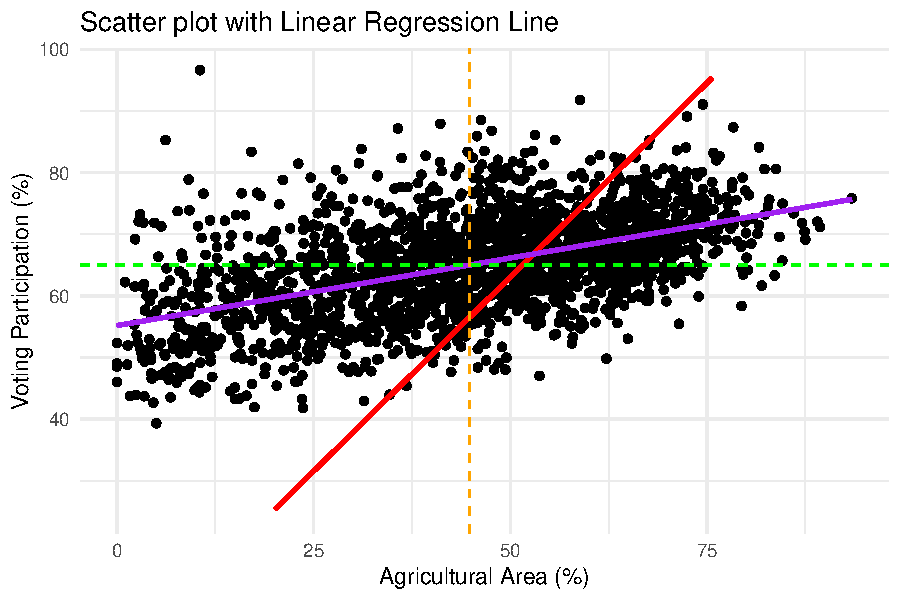
\includegraphics{_main_files/figure-latex/unnamed-chunk-40-1.pdf}

\begin{enumerate}
\def\labelenumi{\roman{enumi}.}
\tightlist
\item
  Store the residualas as \texttt{residuals}. Plot the share of agricultural area against the residuals. What does it tell you regarding the ability of the model to describe the central tendency of the relationship across all values of the agricultural land share?
\end{enumerate}

\begin{Shaded}
\begin{Highlighting}[]
\NormalTok{residuals1 }\OtherTok{\textless{}{-}} \FunctionTok{residuals}\NormalTok{(result1)}

\FunctionTok{ggplot}\NormalTok{(CO2, }\FunctionTok{aes}\NormalTok{(}\AttributeTok{x =}\NormalTok{ AgricAreaPercent, }\AttributeTok{y =}\NormalTok{ residuals1)) }\SpecialCharTok{+}
  \FunctionTok{geom\_point}\NormalTok{() }\SpecialCharTok{+}
  \FunctionTok{geom\_smooth}\NormalTok{(}\AttributeTok{method =} \StringTok{"lm"}\NormalTok{, }\AttributeTok{formula =}\NormalTok{ y }\SpecialCharTok{\textasciitilde{}}\NormalTok{ x , }\AttributeTok{se =} \ConstantTok{TRUE}\NormalTok{, }\AttributeTok{color =} \StringTok{"green"}\NormalTok{)}\SpecialCharTok{+}  \CommentTok{\# Adding the}
  \FunctionTok{theme\_minimal}\NormalTok{() }\SpecialCharTok{+}
  \FunctionTok{labs}\NormalTok{(}
    \AttributeTok{x =} \StringTok{"Agricultural Area (\%)"}\NormalTok{,}
    \AttributeTok{y =} \StringTok{"Residuals (turn{-}out p.p.)"}\NormalTok{,}
    \AttributeTok{title =} \StringTok{"Scatter plot with Linear Regression Line"}
\NormalTok{  )}
\end{Highlighting}
\end{Shaded}

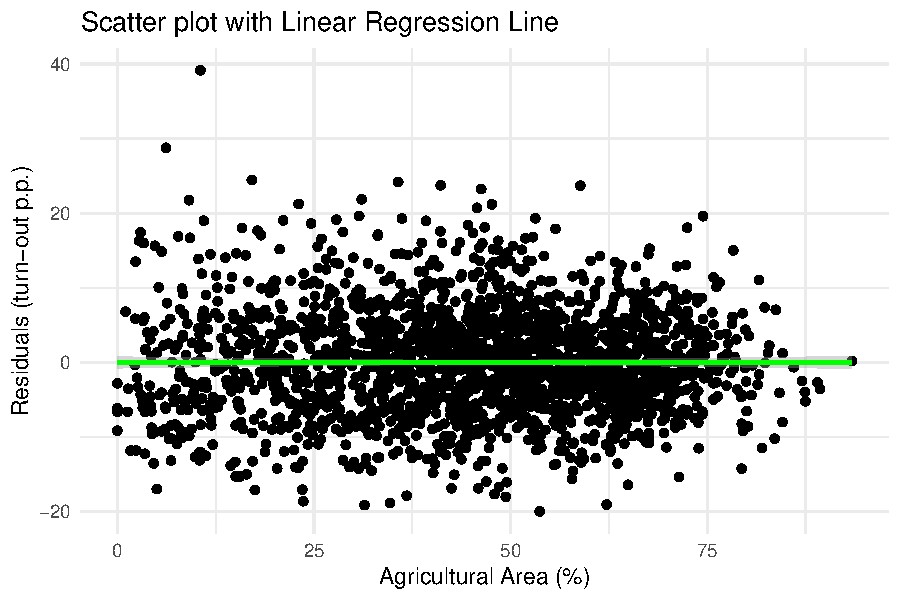
\includegraphics{_main_files/figure-latex/unnamed-chunk-41-1.pdf}

\begin{enumerate}
\def\labelenumi{\roman{enumi}.}
\tightlist
\item
  {[}Optional{]} Repeat the previous point without the intercept. Does the linear regression remains a good tool for describing the central tendency of the relationship across all values of the agricultural land share?
\end{enumerate}

\begin{Shaded}
\begin{Highlighting}[]
\NormalTok{residuals0 }\OtherTok{\textless{}{-}} \FunctionTok{residuals}\NormalTok{(result0)}

\FunctionTok{ggplot}\NormalTok{(CO2, }\FunctionTok{aes}\NormalTok{(}\AttributeTok{x =}\NormalTok{ AgricAreaPercent, }\AttributeTok{y =}\NormalTok{ residuals0)) }\SpecialCharTok{+}
  \FunctionTok{geom\_point}\NormalTok{() }\SpecialCharTok{+}
  \FunctionTok{geom\_smooth}\NormalTok{(}\AttributeTok{method =} \StringTok{"lm"}\NormalTok{, }\AttributeTok{formula =}\NormalTok{ y }\SpecialCharTok{\textasciitilde{}}\NormalTok{ x , }\AttributeTok{se =} \ConstantTok{TRUE}\NormalTok{, }\AttributeTok{color =} \StringTok{"red"}\NormalTok{)}\SpecialCharTok{+}  \CommentTok{\# Adding the}
  \FunctionTok{theme\_minimal}\NormalTok{() }\SpecialCharTok{+}
  \FunctionTok{labs}\NormalTok{(}
    \AttributeTok{x =} \StringTok{"Agricultural Area (\%)"}\NormalTok{,}
    \AttributeTok{y =} \StringTok{"Residuals (turn{-}out p.p.)"}\NormalTok{,}
    \AttributeTok{title =} \StringTok{"Scatter plot with Linear Regression Line"}
\NormalTok{  )}
\end{Highlighting}
\end{Shaded}

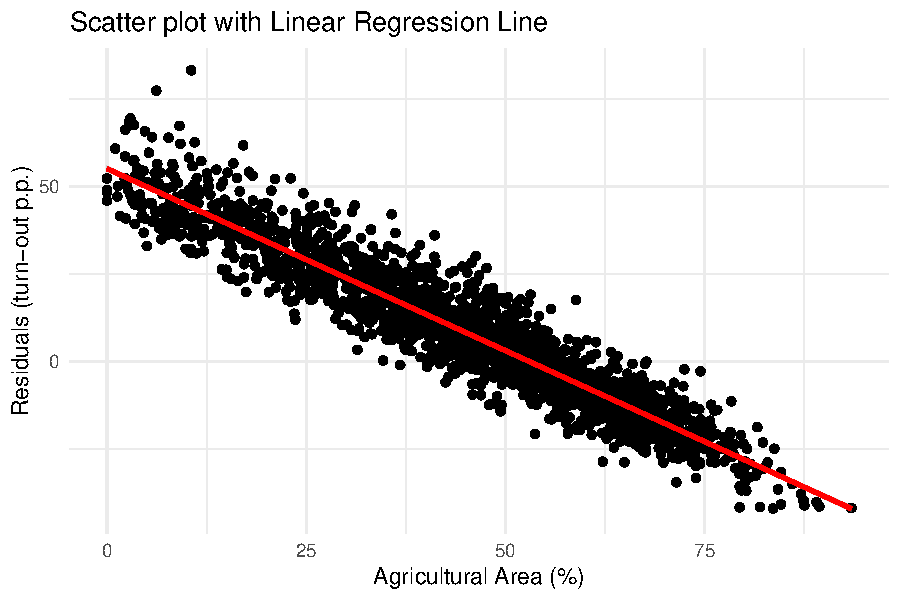
\includegraphics{_main_files/figure-latex/unnamed-chunk-42-1.pdf}

\hypertarget{simulated-data}{%
\subsection{Simulated data}\label{simulated-data}}

\begin{enumerate}
\def\labelenumi{\roman{enumi}.}
\tightlist
\item
  You will now simulate the relationship between turn-out and share of agricultural land. Assume the parameters estimated in the last regression (i.e., the \(\beta_0\) and \(\beta_1\)). Retrieve both parameters.
\end{enumerate}

\begin{Shaded}
\begin{Highlighting}[]
\NormalTok{coeffs}\OtherTok{\textless{}{-}} \FunctionTok{coef}\NormalTok{(result1)}
\FunctionTok{print}\NormalTok{(coeffs)}
\end{Highlighting}
\end{Shaded}

\begin{verbatim}
##      (Intercept) AgricAreaPercent 
##        55.189867         0.219491
\end{verbatim}

\begin{Shaded}
\begin{Highlighting}[]
\FunctionTok{print}\NormalTok{(}\FunctionTok{unname}\NormalTok{(coeffs[}\DecValTok{1}\NormalTok{]), }\AttributeTok{digits =} \DecValTok{5}\NormalTok{)}
\end{Highlighting}
\end{Shaded}

\begin{verbatim}
## [1] 55.19
\end{verbatim}

\begin{Shaded}
\begin{Highlighting}[]
\FunctionTok{print}\NormalTok{(}\FunctionTok{unname}\NormalTok{(coeffs[}\DecValTok{2}\NormalTok{]), }\AttributeTok{digits =} \DecValTok{5}\NormalTok{)}
\end{Highlighting}
\end{Shaded}

\begin{verbatim}
## [1] 0.21949
\end{verbatim}

\begin{enumerate}
\def\labelenumi{\roman{enumi}.}
\tightlist
\item
  Use the parameters to define the assumed data generating process. Assume that the process is deterministic (i.e., it has no stochastic component). Express the equation using mathematical notation.
\end{enumerate}

\[TurnOut_i = \beta_0 + \beta_1 * ShareAgriculturalLand\]

\begin{enumerate}
\def\labelenumi{\roman{enumi}.}
\tightlist
\item
  Generate a normal distribution that preserves the mean and standard deviation of the original data on share of agricultural land.
\end{enumerate}

\begin{Shaded}
\begin{Highlighting}[]
\NormalTok{CO2}\SpecialCharTok{$}\NormalTok{Sim\_ShareAgric\_norm }\OtherTok{\textless{}{-}} \FunctionTok{rnorm}\NormalTok{(}\FunctionTok{nrow}\NormalTok{(CO2), }\AttributeTok{mean =}\NormalTok{ mean\_AgricAreaPercent, }\AttributeTok{sd =} \FunctionTok{sd}\NormalTok{(CO2}\SpecialCharTok{$}\NormalTok{AgricAreaPercent))}

\FunctionTok{hist}\NormalTok{(CO2}\SpecialCharTok{$}\NormalTok{Sim\_ShareAgric\_norm, }
     \AttributeTok{main=}\StringTok{"Histogram of Share of Simulated Agricultural Land"}\NormalTok{, }
     \AttributeTok{xlab=}\StringTok{"Data Values"}\NormalTok{, }
     \AttributeTok{ylab=}\StringTok{"Frequency"}\NormalTok{, }
     \AttributeTok{col=}\StringTok{"blue"}\NormalTok{, }
     \AttributeTok{border=}\StringTok{"black"}\NormalTok{)}

\FunctionTok{abline}\NormalTok{(}\AttributeTok{v=}\NormalTok{mean\_AgricAreaPercent, }\AttributeTok{col=}\StringTok{"red"}\NormalTok{, }\AttributeTok{lwd=}\DecValTok{2}\NormalTok{, }\AttributeTok{lty=}\DecValTok{2}\NormalTok{)}
\end{Highlighting}
\end{Shaded}

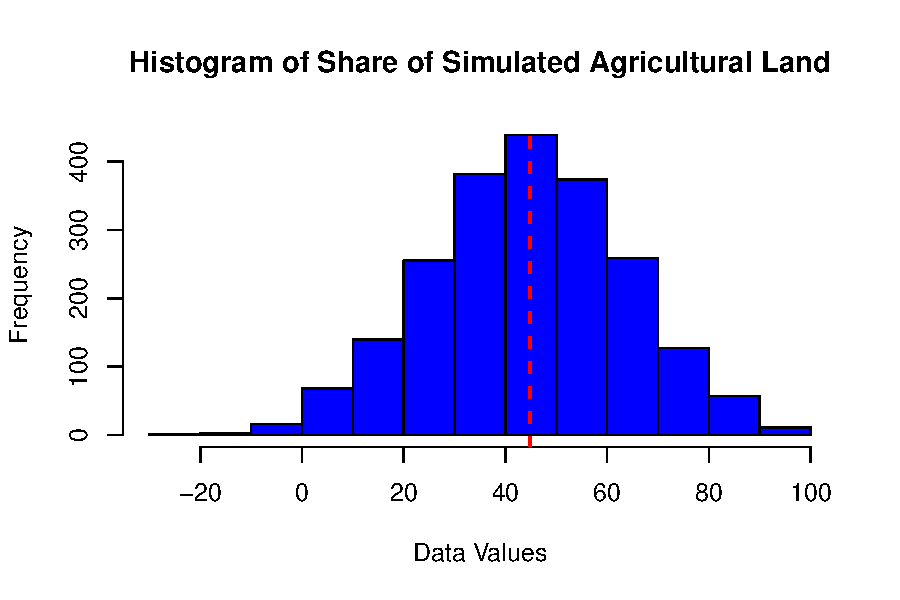
\includegraphics{_main_files/figure-latex/unnamed-chunk-44-1.pdf}

\begin{enumerate}
\def\labelenumi{\roman{enumi}.}
\tightlist
\item
  Predict the turn-out values given the simulated inputs on the share of agricultural land using the data generating process defined two points above. Graph relation between both variables using a liner regression line.
\end{enumerate}

\begin{Shaded}
\begin{Highlighting}[]
\NormalTok{CO2}\SpecialCharTok{$}\NormalTok{Pred\_TurnOut\_Determ }\OtherTok{\textless{}{-}} \FunctionTok{unname}\NormalTok{(coeffs[}\DecValTok{1}\NormalTok{]) }\SpecialCharTok{+} \FunctionTok{unname}\NormalTok{(coeffs[}\DecValTok{2}\NormalTok{])}\SpecialCharTok{*}\NormalTok{CO2}\SpecialCharTok{$}\NormalTok{Sim\_ShareAgric\_norm}


\FunctionTok{ggplot}\NormalTok{(CO2, }\FunctionTok{aes}\NormalTok{(}\AttributeTok{x =}\NormalTok{ Sim\_ShareAgric\_norm, }\AttributeTok{y =}\NormalTok{ Pred\_TurnOut\_Determ)) }\SpecialCharTok{+}
  \FunctionTok{geom\_point}\NormalTok{() }\SpecialCharTok{+}
  \FunctionTok{geom\_smooth}\NormalTok{(}\AttributeTok{method =} \StringTok{"lm"}\NormalTok{, }\AttributeTok{formula =}\NormalTok{ y }\SpecialCharTok{\textasciitilde{}}\NormalTok{ x, }\AttributeTok{se =} \ConstantTok{FALSE}\NormalTok{, }\AttributeTok{color =} \StringTok{"purple"}\NormalTok{) }\SpecialCharTok{+}  \CommentTok{\# Adding the regression line}
  \FunctionTok{geom\_hline}\NormalTok{(}\AttributeTok{yintercept =}\NormalTok{ mean\_stimmbeteiligungInProzent, }\AttributeTok{linetype =} \StringTok{"dashed"}\NormalTok{, }\AttributeTok{color =} \StringTok{"green"}\NormalTok{) }\SpecialCharTok{+}  \CommentTok{\# Horizontal line at the mean of y}
  \FunctionTok{geom\_vline}\NormalTok{(}\AttributeTok{xintercept =}\NormalTok{ mean\_AgricAreaPercent, }\AttributeTok{linetype =} \StringTok{"dashed"}\NormalTok{, }\AttributeTok{color =} \StringTok{"orange"}\NormalTok{) }\SpecialCharTok{+}  \CommentTok{\# Vertical line at the mean of x}
  \FunctionTok{scale\_y\_continuous}\NormalTok{(}\AttributeTok{limits =} \FunctionTok{c}\NormalTok{(}\DecValTok{25}\NormalTok{, }\FunctionTok{max}\NormalTok{(CO2}\SpecialCharTok{$}\NormalTok{stimmbeteiligungInProzent, }\AttributeTok{na.rm =} \ConstantTok{TRUE}\NormalTok{))) }\SpecialCharTok{+}  \CommentTok{\#}
  \FunctionTok{theme\_minimal}\NormalTok{() }\SpecialCharTok{+}
  \FunctionTok{labs}\NormalTok{(}
    \AttributeTok{x =} \StringTok{"Agricultural Area (\%)"}\NormalTok{,}
    \AttributeTok{y =} \StringTok{"Voting Participation (\%)"}\NormalTok{,}
    \AttributeTok{title =} \StringTok{"Simulation: deterministic model"}
\NormalTok{  )}
\end{Highlighting}
\end{Shaded}

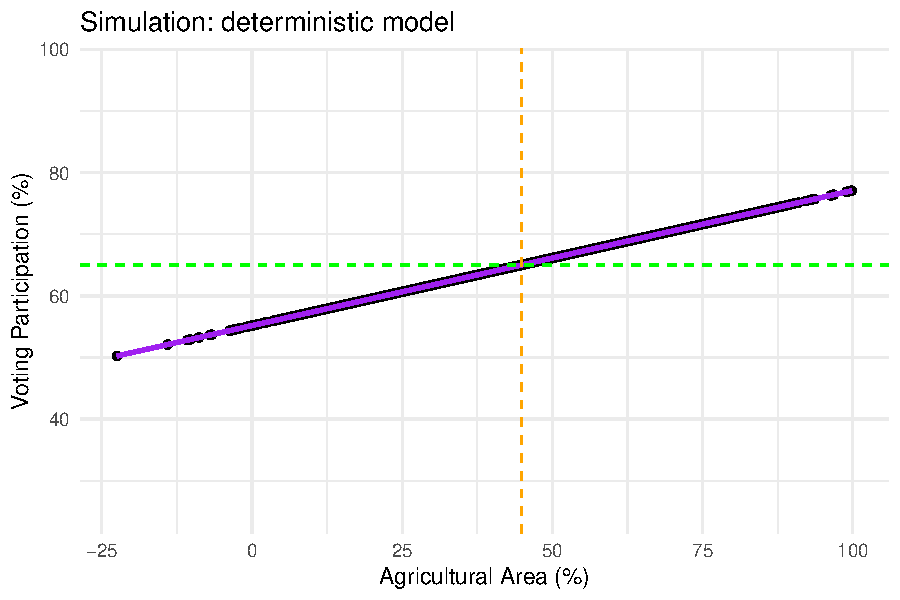
\includegraphics{_main_files/figure-latex/unnamed-chunk-45-1.pdf}

\begin{enumerate}
\def\labelenumi{\roman{enumi}.}
\tightlist
\item
  Generate a normal distribution with error distribution with mean zero and standard deviation equal to the standard deviation of the residual of the model with intercept.
\end{enumerate}

\begin{Shaded}
\begin{Highlighting}[]
\NormalTok{CO2}\SpecialCharTok{$}\NormalTok{Sim\_resid\_norm }\OtherTok{\textless{}{-}} \FunctionTok{rnorm}\NormalTok{(}\FunctionTok{nrow}\NormalTok{(CO2), }\AttributeTok{mean =} \DecValTok{0}\NormalTok{, }\AttributeTok{sd =} \FunctionTok{sd}\NormalTok{(residuals1))}

\FunctionTok{hist}\NormalTok{(CO2}\SpecialCharTok{$}\NormalTok{Sim\_resid\_norm, }
     \AttributeTok{main=}\StringTok{"Histogram of Simulated Normal Residuals"}\NormalTok{, }
     \AttributeTok{xlab=}\StringTok{"Data Values"}\NormalTok{, }
     \AttributeTok{ylab=}\StringTok{"Frequency"}\NormalTok{, }
     \AttributeTok{col=}\StringTok{"blue"}\NormalTok{, }
     \AttributeTok{border=}\StringTok{"black"}\NormalTok{)}

\FunctionTok{abline}\NormalTok{(}\AttributeTok{v=}\DecValTok{0}\NormalTok{, }\AttributeTok{col=}\StringTok{"red"}\NormalTok{, }\AttributeTok{lwd=}\DecValTok{2}\NormalTok{, }\AttributeTok{lty=}\DecValTok{2}\NormalTok{)}
\end{Highlighting}
\end{Shaded}

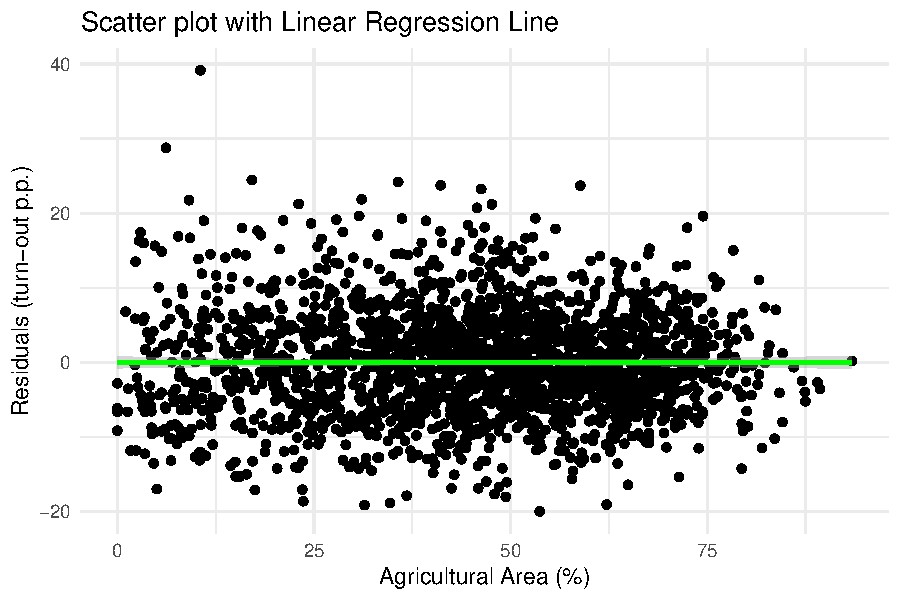
\includegraphics{_main_files/figure-latex/unnamed-chunk-46-1.pdf}

\begin{enumerate}
\def\labelenumi{\roman{enumi}.}
\tightlist
\item
  Repeat the same model but now add the stochastic element. Graph relation between both variables using a liner regression line.
\end{enumerate}

\begin{Shaded}
\begin{Highlighting}[]
\NormalTok{CO2}\SpecialCharTok{$}\NormalTok{Pred\_TurnOut\_Stoch }\OtherTok{\textless{}{-}}\NormalTok{ CO2}\SpecialCharTok{$}\NormalTok{Pred\_TurnOut\_Determ }\SpecialCharTok{+}\NormalTok{ CO2}\SpecialCharTok{$}\NormalTok{Sim\_resid\_norm}



\FunctionTok{ggplot}\NormalTok{(CO2, }\FunctionTok{aes}\NormalTok{(}\AttributeTok{x =}\NormalTok{ Sim\_ShareAgric\_norm, }\AttributeTok{y =}\NormalTok{ Pred\_TurnOut\_Stoch)) }\SpecialCharTok{+}
  \FunctionTok{geom\_point}\NormalTok{() }\SpecialCharTok{+}
  \FunctionTok{geom\_smooth}\NormalTok{(}\AttributeTok{method =} \StringTok{"lm"}\NormalTok{, }\AttributeTok{formula =}\NormalTok{ y }\SpecialCharTok{\textasciitilde{}}\NormalTok{ x, }\AttributeTok{se =} \ConstantTok{FALSE}\NormalTok{, }\AttributeTok{color =} \StringTok{"purple"}\NormalTok{) }\SpecialCharTok{+}  \CommentTok{\# Adding the regression line}
  \FunctionTok{geom\_hline}\NormalTok{(}\AttributeTok{yintercept =}\NormalTok{ mean\_stimmbeteiligungInProzent, }\AttributeTok{linetype =} \StringTok{"dashed"}\NormalTok{, }\AttributeTok{color =} \StringTok{"green"}\NormalTok{) }\SpecialCharTok{+}  \CommentTok{\# Horizontal line at the mean of y}
  \FunctionTok{geom\_vline}\NormalTok{(}\AttributeTok{xintercept =}\NormalTok{ mean\_AgricAreaPercent, }\AttributeTok{linetype =} \StringTok{"dashed"}\NormalTok{, }\AttributeTok{color =} \StringTok{"orange"}\NormalTok{) }\SpecialCharTok{+}  \CommentTok{\# Vertical line at the mean of x}
  \FunctionTok{scale\_y\_continuous}\NormalTok{(}\AttributeTok{limits =} \FunctionTok{c}\NormalTok{(}\DecValTok{25}\NormalTok{, }\FunctionTok{max}\NormalTok{(CO2}\SpecialCharTok{$}\NormalTok{Sim\_ShareAgric\_norm, }\AttributeTok{na.rm =} \ConstantTok{TRUE}\NormalTok{))) }\SpecialCharTok{+}  \CommentTok{\#}
  \FunctionTok{theme\_minimal}\NormalTok{() }\SpecialCharTok{+}
  \FunctionTok{labs}\NormalTok{(}
    \AttributeTok{x =} \StringTok{"Agricultural Area (\%)"}\NormalTok{,}
    \AttributeTok{y =} \StringTok{"Voting Participation (\%)"}\NormalTok{,}
    \AttributeTok{title =} \StringTok{"Simulation: deterministic and stochastic model"}
\NormalTok{  )}
\end{Highlighting}
\end{Shaded}

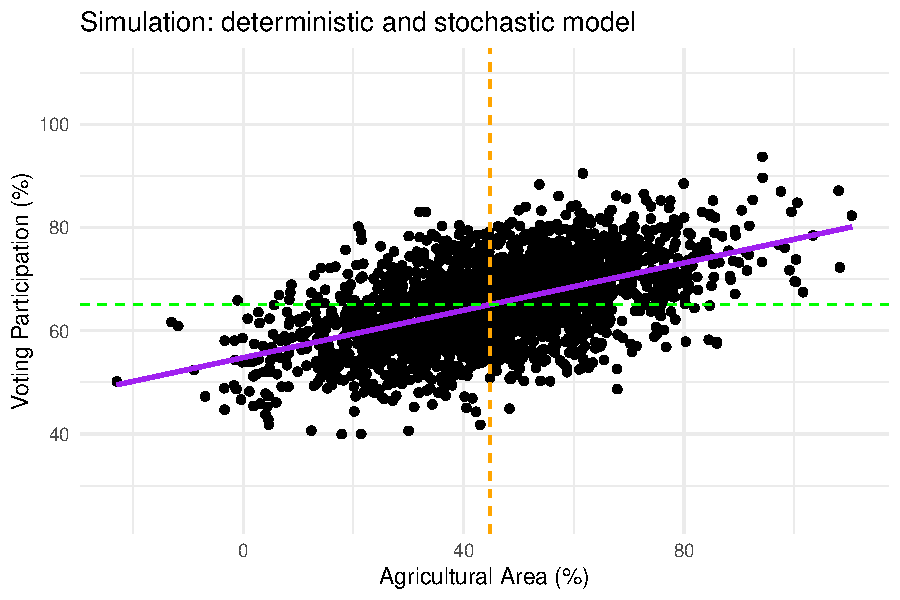
\includegraphics{_main_files/figure-latex/unnamed-chunk-47-1.pdf}

\begin{enumerate}
\def\labelenumi{\roman{enumi}.}
\tightlist
\item
  {[}Optional{]} Now repeat the same simulation but generating errors that distribute uniformly and lognormally. For the lognormal distribution, use the same mean and standard deviations as in the immediately previous exercises. For the uniform, use the maximum, and minimum values of the residuals for the model with intercept.
\end{enumerate}

Uniform simulated residuals:

\begin{Shaded}
\begin{Highlighting}[]
\NormalTok{CO2}\SpecialCharTok{$}\NormalTok{Sim\_resid\_unif }\OtherTok{\textless{}{-}} \FunctionTok{runif}\NormalTok{(}\FunctionTok{nrow}\NormalTok{(CO2), }\AttributeTok{min =} \FunctionTok{min}\NormalTok{(residuals1), }\AttributeTok{max =} \FunctionTok{max}\NormalTok{(residuals1))}

\FunctionTok{hist}\NormalTok{(CO2}\SpecialCharTok{$}\NormalTok{Sim\_resid\_unif, }
     \AttributeTok{main=}\StringTok{"Histogram of Simulated Uniform Residuals"}\NormalTok{, }
     \AttributeTok{xlab=}\StringTok{"Data Values"}\NormalTok{, }
     \AttributeTok{ylab=}\StringTok{"Frequency"}\NormalTok{, }
     \AttributeTok{col=}\StringTok{"blue"}\NormalTok{, }
     \AttributeTok{border=}\StringTok{"black"}\NormalTok{)}

\FunctionTok{abline}\NormalTok{(}\AttributeTok{v=}\DecValTok{0}\NormalTok{, }\AttributeTok{col=}\StringTok{"red"}\NormalTok{, }\AttributeTok{lwd=}\DecValTok{2}\NormalTok{, }\AttributeTok{lty=}\DecValTok{2}\NormalTok{)}
\end{Highlighting}
\end{Shaded}

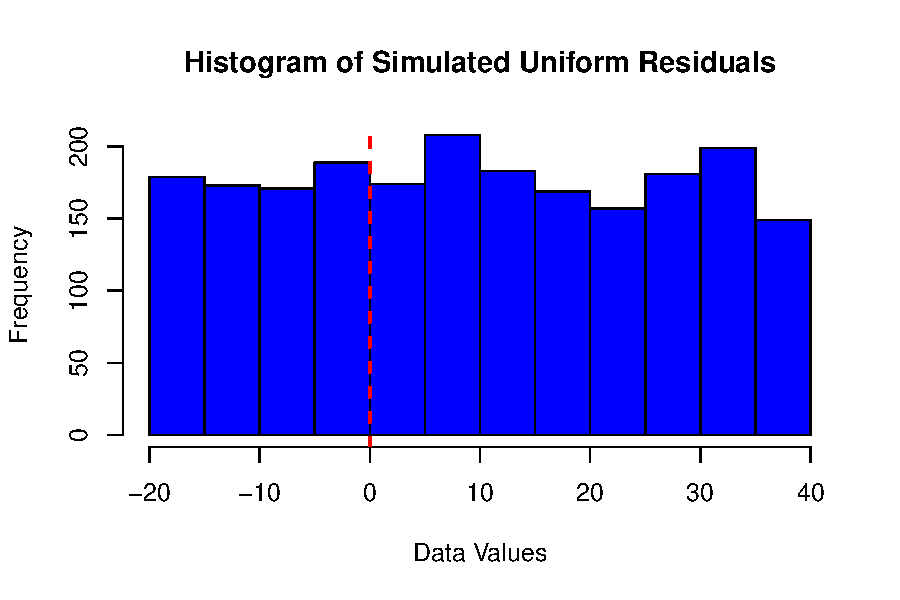
\includegraphics{_main_files/figure-latex/unnamed-chunk-48-1.pdf}

Data generating process with uniform residuals:

\begin{Shaded}
\begin{Highlighting}[]
\NormalTok{CO2}\SpecialCharTok{$}\NormalTok{Pred\_TurnOut\_Unif }\OtherTok{\textless{}{-}}\NormalTok{ CO2}\SpecialCharTok{$}\NormalTok{Pred\_TurnOut\_Determ }\SpecialCharTok{+}\NormalTok{ CO2}\SpecialCharTok{$}\NormalTok{Sim\_resid\_unif}



\FunctionTok{ggplot}\NormalTok{(CO2, }\FunctionTok{aes}\NormalTok{(}\AttributeTok{x =}\NormalTok{ Sim\_ShareAgric\_norm, }\AttributeTok{y =}\NormalTok{ Pred\_TurnOut\_Unif)) }\SpecialCharTok{+}
  \FunctionTok{geom\_point}\NormalTok{() }\SpecialCharTok{+}
  \FunctionTok{geom\_smooth}\NormalTok{(}\AttributeTok{method =} \StringTok{"lm"}\NormalTok{, }\AttributeTok{formula =}\NormalTok{ y }\SpecialCharTok{\textasciitilde{}}\NormalTok{ x, }\AttributeTok{se =} \ConstantTok{FALSE}\NormalTok{, }\AttributeTok{color =} \StringTok{"purple"}\NormalTok{) }\SpecialCharTok{+} 
  \FunctionTok{geom\_hline}\NormalTok{(}\AttributeTok{yintercept =} \FunctionTok{mean}\NormalTok{(CO2}\SpecialCharTok{$}\NormalTok{Pred\_TurnOut\_Unif), }\AttributeTok{linetype =} \StringTok{"dashed"}\NormalTok{, }\AttributeTok{color =} \StringTok{"green"}\NormalTok{) }\SpecialCharTok{+}  
  \FunctionTok{geom\_vline}\NormalTok{(}\AttributeTok{xintercept =}\NormalTok{ mean\_AgricAreaPercent, }\AttributeTok{linetype =} \StringTok{"dashed"}\NormalTok{, }\AttributeTok{color =} \StringTok{"orange"}\NormalTok{) }\SpecialCharTok{+}  
  \FunctionTok{scale\_y\_continuous}\NormalTok{(}\AttributeTok{limits =} \FunctionTok{c}\NormalTok{(}\DecValTok{25}\NormalTok{, }\FunctionTok{max}\NormalTok{(CO2}\SpecialCharTok{$}\NormalTok{Pred\_TurnOut\_Unif, }\AttributeTok{na.rm =} \ConstantTok{TRUE}\NormalTok{))) }\SpecialCharTok{+}  
  \FunctionTok{theme\_minimal}\NormalTok{() }\SpecialCharTok{+}
  \FunctionTok{labs}\NormalTok{(}
    \AttributeTok{x =} \StringTok{"Agricultural Area (\%)"}\NormalTok{,}
    \AttributeTok{y =} \StringTok{"Voting Participation (\%)"}\NormalTok{,}
    \AttributeTok{title =} \StringTok{"Simulation: deterministic and stochastic model (uniform error)"}
\NormalTok{  )}
\end{Highlighting}
\end{Shaded}

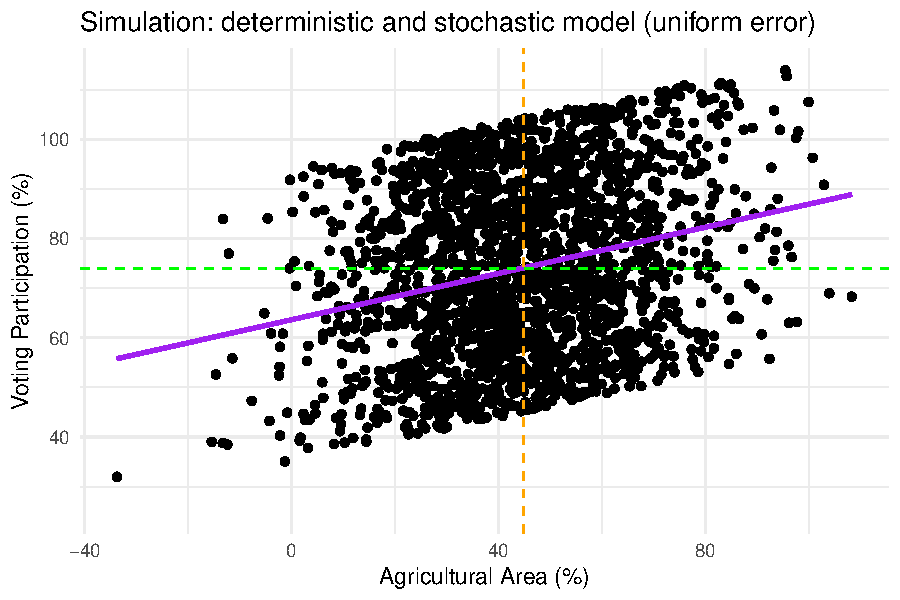
\includegraphics{_main_files/figure-latex/unnamed-chunk-49-1.pdf}

Lognormal simulated residuals:

\begin{Shaded}
\begin{Highlighting}[]
\NormalTok{CO2}\SpecialCharTok{$}\NormalTok{Sim\_resid\_lnorm }\OtherTok{\textless{}{-}} \FunctionTok{rlnorm}\NormalTok{(}\FunctionTok{nrow}\NormalTok{(CO2), }\AttributeTok{mean =} \DecValTok{0}\NormalTok{, }\AttributeTok{sd =} \FunctionTok{sd}\NormalTok{(residuals1))}



\FunctionTok{hist}\NormalTok{(CO2}\SpecialCharTok{$}\NormalTok{Sim\_resid\_lnorm, }
     \AttributeTok{main=}\StringTok{"Histogram of Simulated Uniform Residuals"}\NormalTok{, }
     \AttributeTok{xlab=}\StringTok{"Data Values"}\NormalTok{, }
     \AttributeTok{ylab=}\StringTok{"Frequency"}\NormalTok{, }
     \AttributeTok{col=}\StringTok{"blue"}\NormalTok{, }
     \AttributeTok{border=}\StringTok{"black"}\NormalTok{)}

\FunctionTok{abline}\NormalTok{(}\AttributeTok{v=}\DecValTok{0}\NormalTok{, }\AttributeTok{col=}\StringTok{"red"}\NormalTok{, }\AttributeTok{lwd=}\DecValTok{2}\NormalTok{, }\AttributeTok{lty=}\DecValTok{2}\NormalTok{)}
\end{Highlighting}
\end{Shaded}

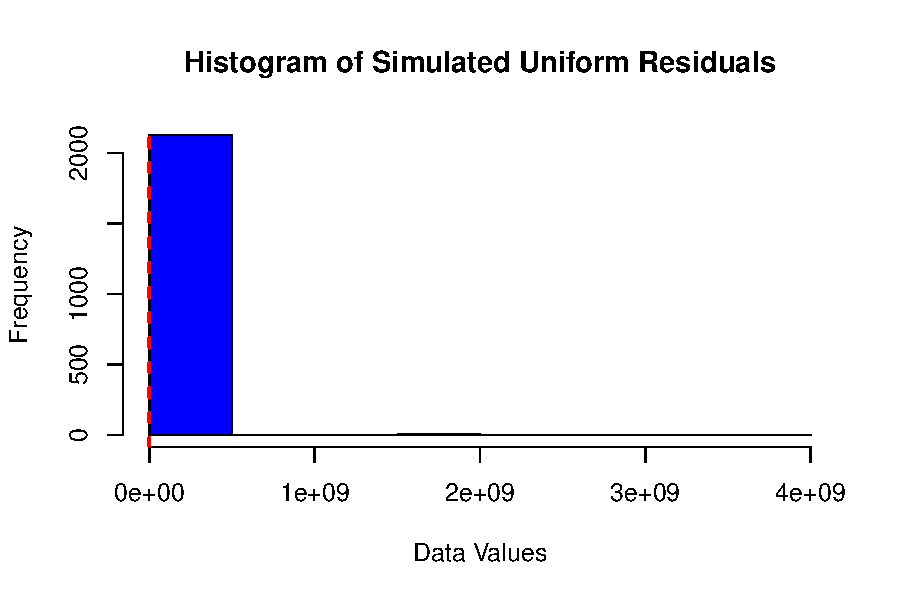
\includegraphics{_main_files/figure-latex/unnamed-chunk-50-1.pdf}

Data generating process with lognormal residuals without adjusting scale of Y:

\begin{Shaded}
\begin{Highlighting}[]
\NormalTok{CO2}\SpecialCharTok{$}\NormalTok{Pred\_TurnOut\_Lnorm }\OtherTok{\textless{}{-}}\NormalTok{ CO2}\SpecialCharTok{$}\NormalTok{Pred\_TurnOut\_Determ }\SpecialCharTok{+}\NormalTok{ CO2}\SpecialCharTok{$}\NormalTok{Sim\_resid\_lnorm}



\FunctionTok{ggplot}\NormalTok{(CO2, }\FunctionTok{aes}\NormalTok{(}\AttributeTok{x =}\NormalTok{ Sim\_ShareAgric\_norm, }\AttributeTok{y =}\NormalTok{ Pred\_TurnOut\_Lnorm)) }\SpecialCharTok{+}
  \FunctionTok{geom\_point}\NormalTok{() }\SpecialCharTok{+}
  \FunctionTok{geom\_smooth}\NormalTok{(}\AttributeTok{method =} \StringTok{"lm"}\NormalTok{, }\AttributeTok{formula =}\NormalTok{ y }\SpecialCharTok{\textasciitilde{}}\NormalTok{ x, }\AttributeTok{se =} \ConstantTok{FALSE}\NormalTok{, }\AttributeTok{color =} \StringTok{"purple"}\NormalTok{) }\SpecialCharTok{+} 
  \FunctionTok{geom\_hline}\NormalTok{(}\AttributeTok{yintercept =} \FunctionTok{mean}\NormalTok{(CO2}\SpecialCharTok{$}\NormalTok{Pred\_TurnOut\_Lnorm), }\AttributeTok{linetype =} \StringTok{"dashed"}\NormalTok{, }\AttributeTok{color =} \StringTok{"green"}\NormalTok{) }\SpecialCharTok{+}  
  \FunctionTok{geom\_vline}\NormalTok{(}\AttributeTok{xintercept =}\NormalTok{ mean\_AgricAreaPercent, }\AttributeTok{linetype =} \StringTok{"dashed"}\NormalTok{, }\AttributeTok{color =} \StringTok{"orange"}\NormalTok{) }\SpecialCharTok{+}  
  \FunctionTok{scale\_y\_continuous}\NormalTok{(}\AttributeTok{limits =} \FunctionTok{c}\NormalTok{(}\DecValTok{25}\NormalTok{, }\FunctionTok{max}\NormalTok{(CO2}\SpecialCharTok{$}\NormalTok{Pred\_TurnOut\_Lnorm, }\AttributeTok{na.rm =} \ConstantTok{TRUE}\NormalTok{))) }\SpecialCharTok{+}  \CommentTok{\#}
  \FunctionTok{theme\_minimal}\NormalTok{() }\SpecialCharTok{+}
  \FunctionTok{labs}\NormalTok{(}
    \AttributeTok{x =} \StringTok{"Agricultural Area (\%)"}\NormalTok{,}
    \AttributeTok{y =} \StringTok{"Voting Participation (\%)"}\NormalTok{,}
    \AttributeTok{title =} \StringTok{"Simulation: deterministic and stochastic model (log normal error)"}
\NormalTok{  )}
\end{Highlighting}
\end{Shaded}

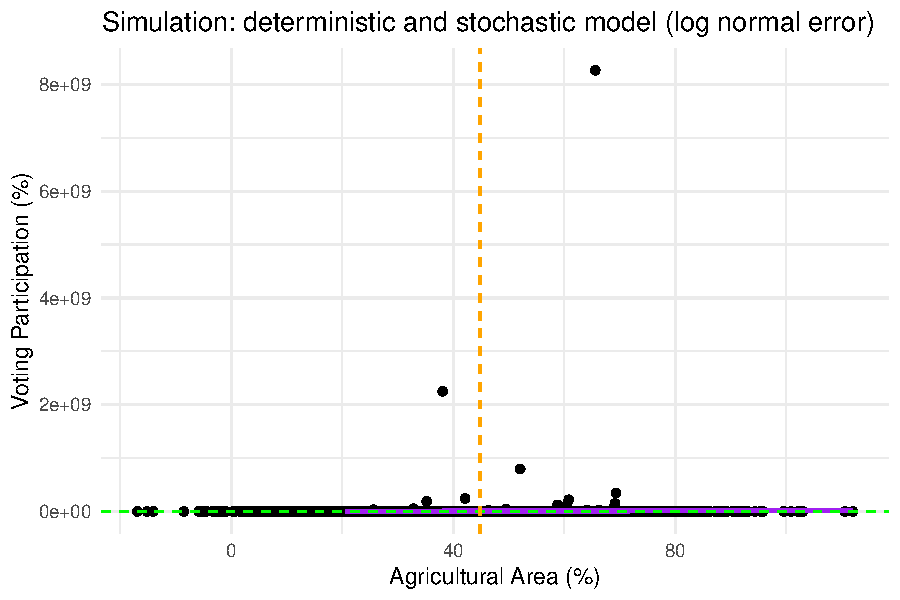
\includegraphics{_main_files/figure-latex/unnamed-chunk-51-1.pdf}
Data generating process with lognormal residuals adjusting scale of Y:

\begin{Shaded}
\begin{Highlighting}[]
\NormalTok{CO2}\SpecialCharTok{$}\NormalTok{Pred\_TurnOut\_Lnorm }\OtherTok{\textless{}{-}}\NormalTok{ CO2}\SpecialCharTok{$}\NormalTok{Pred\_TurnOut\_Determ }\SpecialCharTok{+}\NormalTok{ CO2}\SpecialCharTok{$}\NormalTok{Sim\_resid\_lnorm}



\FunctionTok{ggplot}\NormalTok{(CO2, }\FunctionTok{aes}\NormalTok{(}\AttributeTok{x =}\NormalTok{ Sim\_ShareAgric\_norm, }\AttributeTok{y =}\NormalTok{ Pred\_TurnOut\_Lnorm)) }\SpecialCharTok{+}
  \FunctionTok{geom\_point}\NormalTok{() }\SpecialCharTok{+}
  \FunctionTok{scale\_y\_log10}\NormalTok{() }\SpecialCharTok{+}
  \FunctionTok{geom\_smooth}\NormalTok{(}\AttributeTok{method =} \StringTok{"lm"}\NormalTok{, }\AttributeTok{formula =}\NormalTok{ y }\SpecialCharTok{\textasciitilde{}}\NormalTok{ x, }\AttributeTok{se =} \ConstantTok{FALSE}\NormalTok{, }\AttributeTok{color =} \StringTok{"purple"}\NormalTok{) }\SpecialCharTok{+}  
  \FunctionTok{geom\_hline}\NormalTok{(}\AttributeTok{yintercept =} \FunctionTok{mean}\NormalTok{(CO2}\SpecialCharTok{$}\NormalTok{Pred\_TurnOut\_Lnorm), }\AttributeTok{linetype =} \StringTok{"dashed"}\NormalTok{, }\AttributeTok{color =} \StringTok{"green"}\NormalTok{) }\SpecialCharTok{+}  
  \FunctionTok{geom\_vline}\NormalTok{(}\AttributeTok{xintercept =}\NormalTok{ mean\_AgricAreaPercent, }\AttributeTok{linetype =} \StringTok{"dashed"}\NormalTok{, }\AttributeTok{color =} \StringTok{"orange"}\NormalTok{) }\SpecialCharTok{+}  
  \FunctionTok{theme\_minimal}\NormalTok{() }\SpecialCharTok{+}
  \FunctionTok{labs}\NormalTok{(}
    \AttributeTok{x =} \StringTok{"Agricultural Area (\%)"}\NormalTok{,}
    \AttributeTok{y =} \StringTok{"Voting Participation (\%) in logarithmic scale"}\NormalTok{,}
    \AttributeTok{title =} \StringTok{"Simulation: deterministic and stochastic model (log normal error)"}
\NormalTok{  )}
\end{Highlighting}
\end{Shaded}

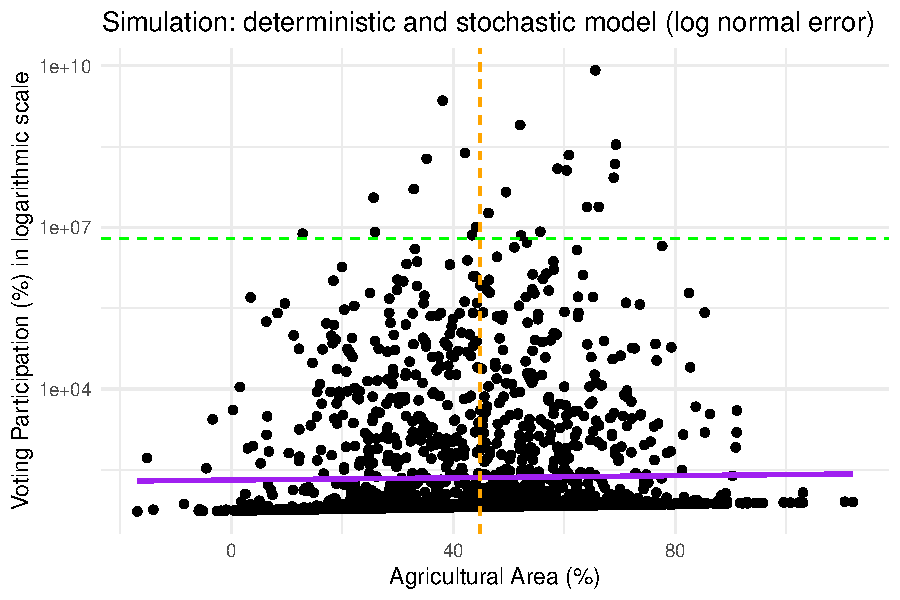
\includegraphics{_main_files/figure-latex/unnamed-chunk-52-1.pdf}
Ask yourself: does it make sense to have participation values higher than 100\%?

Parabolic simulated residuals:

\begin{Shaded}
\begin{Highlighting}[]
\NormalTok{CO2}\SpecialCharTok{$}\NormalTok{parab\_norm\_resid}\OtherTok{\textless{}{-}} \SpecialCharTok{{-}}\FloatTok{0.01}\SpecialCharTok{*}\NormalTok{(CO2}\SpecialCharTok{$}\NormalTok{Sim\_ShareAgric\_norm}\SpecialCharTok{{-}}\FunctionTok{mean}\NormalTok{(CO2}\SpecialCharTok{$}\NormalTok{Sim\_ShareAgric\_norm))}\SpecialCharTok{\^{}}\DecValTok{2}\SpecialCharTok{+}\NormalTok{CO2}\SpecialCharTok{$}\NormalTok{Sim\_resid\_norm}
\NormalTok{CO2}\SpecialCharTok{$}\NormalTok{parab\_norm\_resid}\OtherTok{\textless{}{-}}\NormalTok{ CO2}\SpecialCharTok{$}\NormalTok{parab\_norm\_resid}\SpecialCharTok{{-}}\FunctionTok{mean}\NormalTok{(CO2}\SpecialCharTok{$}\NormalTok{parab\_norm\_resid)}


\FunctionTok{ggplot}\NormalTok{(CO2, }\FunctionTok{aes}\NormalTok{(}\AttributeTok{x =}\NormalTok{ Sim\_ShareAgric\_norm, }\AttributeTok{y =}\NormalTok{ parab\_norm\_resid)) }\SpecialCharTok{+}
  \FunctionTok{geom\_point}\NormalTok{() }\SpecialCharTok{+}
  \FunctionTok{geom\_smooth}\NormalTok{(}\AttributeTok{method =} \StringTok{"lm"}\NormalTok{, }\AttributeTok{formula =}\NormalTok{ y }\SpecialCharTok{\textasciitilde{}}\NormalTok{ x, }\AttributeTok{se =} \ConstantTok{FALSE}\NormalTok{, }\AttributeTok{color =} \StringTok{"green"}\NormalTok{) }\SpecialCharTok{+}
  \FunctionTok{theme\_minimal}\NormalTok{() }\SpecialCharTok{+}
  \FunctionTok{labs}\NormalTok{(}
    \AttributeTok{x =} \StringTok{"Agricultural Area (\%)"}\NormalTok{,}
    \AttributeTok{y =} \StringTok{"Error"}\NormalTok{,}
    \AttributeTok{title =} \StringTok{"Simulation: of parabolic error"}
\NormalTok{  )}
\end{Highlighting}
\end{Shaded}

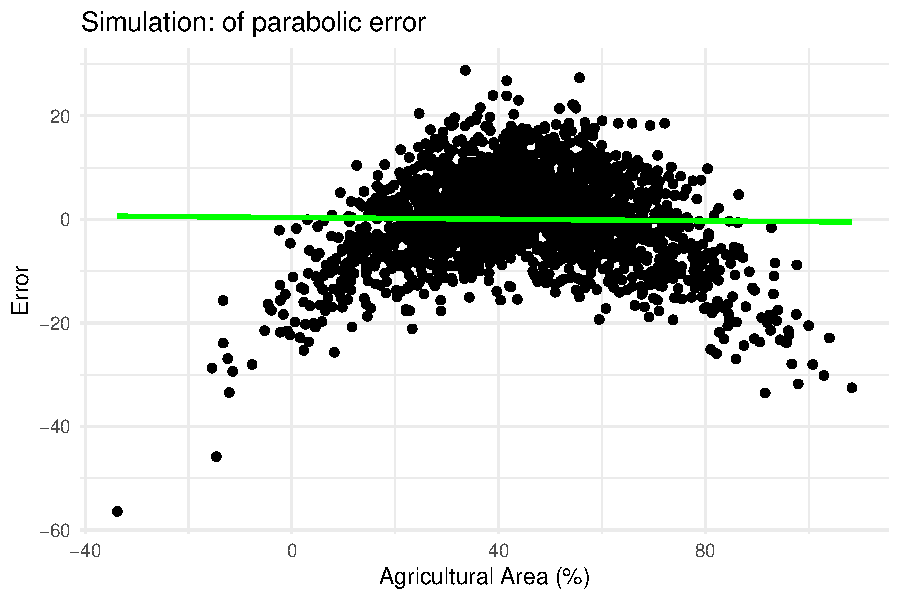
\includegraphics{_main_files/figure-latex/unnamed-chunk-53-1.pdf}
What does the behavior of the error tell you about the potential reliability of a regression without quadratic terms?

Data generating process with parabolic residuals:

\begin{Shaded}
\begin{Highlighting}[]
\NormalTok{CO2}\SpecialCharTok{$}\NormalTok{Pred\_TurnOut\_parab\_norm\_resid }\OtherTok{\textless{}{-}}\NormalTok{ CO2}\SpecialCharTok{$}\NormalTok{Pred\_TurnOut\_Determ }\SpecialCharTok{+}\NormalTok{ CO2}\SpecialCharTok{$}\NormalTok{parab\_norm\_resid}



\FunctionTok{ggplot}\NormalTok{(CO2, }\FunctionTok{aes}\NormalTok{(}\AttributeTok{x =}\NormalTok{ Sim\_ShareAgric\_norm, }\AttributeTok{y =}\NormalTok{ Pred\_TurnOut\_parab\_norm\_resid)) }\SpecialCharTok{+}
  \FunctionTok{geom\_point}\NormalTok{() }\SpecialCharTok{+}
  \FunctionTok{geom\_smooth}\NormalTok{(}\AttributeTok{method =} \StringTok{"lm"}\NormalTok{, }\AttributeTok{formula =}\NormalTok{ y }\SpecialCharTok{\textasciitilde{}}\NormalTok{ x, }\AttributeTok{se =} \ConstantTok{FALSE}\NormalTok{, }\AttributeTok{color =} \StringTok{"purple"}\NormalTok{) }\SpecialCharTok{+}
  \FunctionTok{geom\_hline}\NormalTok{(}\AttributeTok{yintercept =} \FunctionTok{mean}\NormalTok{(CO2}\SpecialCharTok{$}\NormalTok{Pred\_TurnOut\_parab\_norm\_resid), }\AttributeTok{linetype =} \StringTok{"dashed"}\NormalTok{, }\AttributeTok{color =} \StringTok{"green"}\NormalTok{) }\SpecialCharTok{+} 
  \FunctionTok{geom\_vline}\NormalTok{(}\AttributeTok{xintercept =}\NormalTok{ mean\_AgricAreaPercent, }\AttributeTok{linetype =} \StringTok{"dashed"}\NormalTok{, }\AttributeTok{color =} \StringTok{"orange"}\NormalTok{) }\SpecialCharTok{+} 
  \FunctionTok{scale\_y\_continuous}\NormalTok{(}\AttributeTok{limits =} \FunctionTok{c}\NormalTok{(}\DecValTok{25}\NormalTok{, }\FunctionTok{max}\NormalTok{(CO2}\SpecialCharTok{$}\NormalTok{Pred\_TurnOut\_Unif, }\AttributeTok{na.rm =} \ConstantTok{TRUE}\NormalTok{))) }\SpecialCharTok{+}  \CommentTok{\#}
  \FunctionTok{theme\_minimal}\NormalTok{() }\SpecialCharTok{+}
  \FunctionTok{labs}\NormalTok{(}
    \AttributeTok{x =} \StringTok{"Agricultural Area (\%)"}\NormalTok{,}
    \AttributeTok{y =} \StringTok{"Voting Participation (\%)"}\NormalTok{,}
    \AttributeTok{title =} \StringTok{"Simulation: deterministic and stochastic model (uniform error)"}
\NormalTok{  )}
\end{Highlighting}
\end{Shaded}

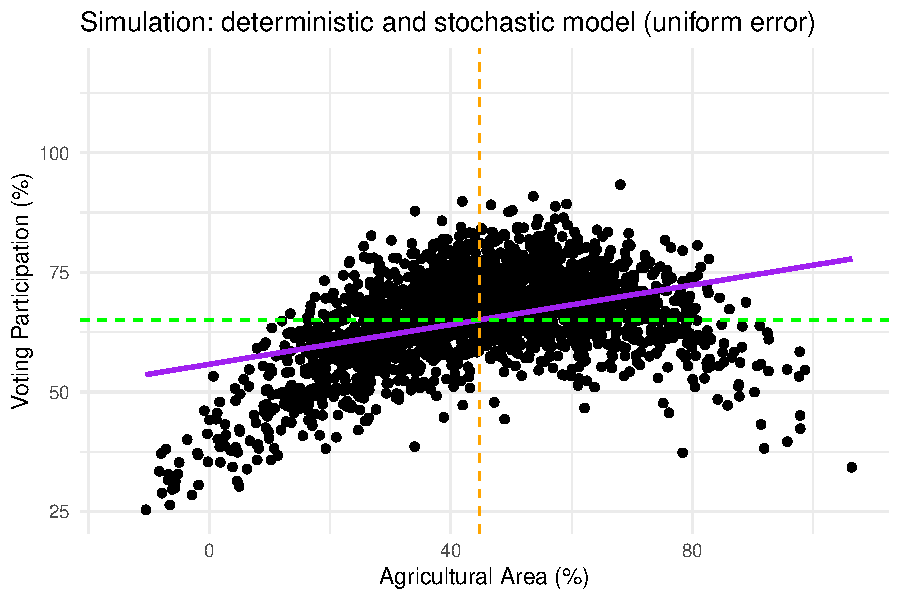
\includegraphics{_main_files/figure-latex/unnamed-chunk-54-1.pdf}
Would using a quadratic term in the regression produce a better fit? Graph the regression line with a quadratic term.

\begin{Shaded}
\begin{Highlighting}[]
\FunctionTok{ggplot}\NormalTok{(CO2, }\FunctionTok{aes}\NormalTok{(}\AttributeTok{x =}\NormalTok{ Sim\_ShareAgric\_norm, }\AttributeTok{y =}\NormalTok{ Pred\_TurnOut\_parab\_norm\_resid)) }\SpecialCharTok{+}
  \FunctionTok{geom\_point}\NormalTok{() }\SpecialCharTok{+}
  \FunctionTok{geom\_smooth}\NormalTok{(}\AttributeTok{method =} \StringTok{"lm"}\NormalTok{, }\AttributeTok{formula =}\NormalTok{ y }\SpecialCharTok{\textasciitilde{}}\NormalTok{ x }\SpecialCharTok{+} \FunctionTok{I}\NormalTok{(x}\SpecialCharTok{\^{}}\DecValTok{2}\NormalTok{), }\AttributeTok{se =} \ConstantTok{FALSE}\NormalTok{, }\AttributeTok{color =} \StringTok{"purple"}\NormalTok{) }\SpecialCharTok{+}
  \FunctionTok{geom\_hline}\NormalTok{(}\AttributeTok{yintercept =} \FunctionTok{mean}\NormalTok{(CO2}\SpecialCharTok{$}\NormalTok{Pred\_TurnOut\_parab\_norm\_resid), }\AttributeTok{linetype =} \StringTok{"dashed"}\NormalTok{, }\AttributeTok{color =} \StringTok{"green"}\NormalTok{) }\SpecialCharTok{+} 
  \FunctionTok{geom\_vline}\NormalTok{(}\AttributeTok{xintercept =}\NormalTok{ mean\_AgricAreaPercent, }\AttributeTok{linetype =} \StringTok{"dashed"}\NormalTok{, }\AttributeTok{color =} \StringTok{"orange"}\NormalTok{) }\SpecialCharTok{+}  
  \FunctionTok{scale\_y\_continuous}\NormalTok{(}\AttributeTok{limits =} \FunctionTok{c}\NormalTok{(}\DecValTok{25}\NormalTok{, }\FunctionTok{max}\NormalTok{(CO2}\SpecialCharTok{$}\NormalTok{Pred\_TurnOut\_Unif, }\AttributeTok{na.rm =} \ConstantTok{TRUE}\NormalTok{))) }\SpecialCharTok{+}  
  \FunctionTok{theme\_minimal}\NormalTok{() }\SpecialCharTok{+}
  \FunctionTok{labs}\NormalTok{(}
    \AttributeTok{x =} \StringTok{"Agricultural Area (\%)"}\NormalTok{,}
    \AttributeTok{y =} \StringTok{"Voting Participation (\%)"}\NormalTok{,}
    \AttributeTok{title =} \StringTok{"Simulation: deterministic and stochastic model (uniform error)"}
\NormalTok{  )}
\end{Highlighting}
\end{Shaded}

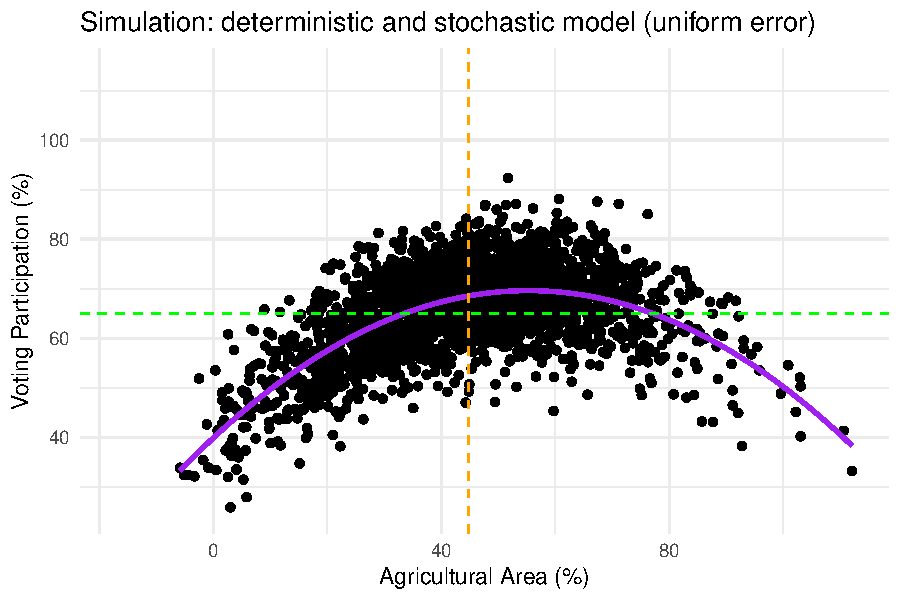
\includegraphics{_main_files/figure-latex/unnamed-chunk-55-1.pdf}

\hypertarget{week-4-regression-ii-model-specification}{%
\chapter{Week 4: Regression II (Model Specification)}\label{week-4-regression-ii-model-specification}}

\hypertarget{aims-2}{%
\section{Aims}\label{aims-2}}

\begin{enumerate}
\def\labelenumi{\arabic{enumi}.}
\tightlist
\item
  Using multiple regressors and interaction terms in regression analysis for quantitative descriptive purposes with real data
\item
  Using simulation to instantiate how different properties of the data generating process alter or not metrics of goodness of fit
\end{enumerate}

\emph{{Should we request them to do descriptive statistics?}.}
\emph{{Check: are all list numerals fine?}.}
\emph{{Check: do all parameters in the interpretation texts fine?}.}

\hypertarget{exercise-context-and-questions}{%
\section{Exercise: Context and Questions}\label{exercise-context-and-questions}}

Currently led by \href{https://forscenter.ch/staff/anke-tresch/}{Prof.~Anke Tresch}, ``{[}t{]}he Swiss Election Study (Selects) has been investigating the electoral behaviour of Swiss citizens in national elections since 1995. The project sheds light on the dynamics of the citizens' opinion formation as well as on the determinants of their political participation and voting choice for a specific candidate or party.'' See more \href{https://forscenter.ch/projects/selects/}{here}.

In this exercise, you will use data for the year 2019. You will use it to answer the following questions:

\begin{enumerate}
\def\labelenumi{\arabic{enumi}.}
\tightlist
\item
  Do older voters have stronger right leaning preferences than younger ones? age
\item
  Does that behavior change across sexes? sex
\item
  Does that behavior change depending on the main language spoken at the respondent's home? f20221
\item
  What about the interaction sex-age?
\item
  What about the interaction sex-language?
\item
  What about the interaction age-language?
\item
  What about the interaction sex-age-language?
\item
  Do right leaning preferences become stronger the older voters are?
\end{enumerate}

\hypertarget{getting-the-data-first-1}{%
\section{Getting the data first}\label{getting-the-data-first-1}}

Opening:

\begin{Shaded}
\begin{Highlighting}[]
\CommentTok{\# selects19 \textless{}{-} read.csv("\textasciitilde{}/Documents/0\_IPZ/2023\_2/Leemann{-}QuantMethods/QuantitativeMethods/Data/SELECTS 2019/1179\_Selects2019\_PES\_Data\_v1.1.0.csv", header = TRUE)}
\CommentTok{\# }
\CommentTok{\# selects19 \textless{}{-} selects19 \%\textgreater{}\%}
\CommentTok{\#   select(sex, age, matches("f15200"), f20221) \%\textgreater{}\%}
\CommentTok{\#   filter(!is.na(selects19$sex) \& !is.na(selects19$age) \& !is.na(selects19$f15200) \& !is.na(selects19$f20221))  \# Remove rows where x or y is NA}
\CommentTok{\# }
\CommentTok{\# selects19$f15200 \textless{}{-} as.numeric(selects19$f15200)}
\CommentTok{\# }
\CommentTok{\# write.table(selects19, file = "\textasciitilde{}/Documents/0\_IPZ/2023\_2/Leemann{-}QuantMethods/QuantitativeMethods/QuantitativeMethods/Data/SELECTS 2019/data.csv", sep = ",", row.names = FALSE)}

\NormalTok{selects19 }\OtherTok{\textless{}{-}} \FunctionTok{read.csv}\NormalTok{(}\StringTok{"\textasciitilde{}/Documents/0\_IPZ/2023\_2/Leemann{-}QuantMethods/QuantitativeMethods/QuantitativeMethods/Data/SELECTS 2019/data.csv"}\NormalTok{, }\AttributeTok{header =} \ConstantTok{TRUE}\NormalTok{)}
\end{Highlighting}
\end{Shaded}

Labeling languages:

\begin{Shaded}
\begin{Highlighting}[]
\NormalTok{selects19 }\OtherTok{\textless{}{-}}\NormalTok{ selects19 }\SpecialCharTok{\%\textgreater{}\%}
  \FunctionTok{mutate}\NormalTok{(}\AttributeTok{LanguageHome =} \FunctionTok{case\_when}\NormalTok{(}
\NormalTok{    f20221 }\SpecialCharTok{==} \DecValTok{1} \SpecialCharTok{\textasciitilde{}} \StringTok{"German/Swiss German"}\NormalTok{,}
\NormalTok{    f20221 }\SpecialCharTok{==} \DecValTok{2} \SpecialCharTok{\textasciitilde{}} \StringTok{"French"}\NormalTok{,}
\NormalTok{    f20221 }\SpecialCharTok{==} \DecValTok{3} \SpecialCharTok{\textasciitilde{}} \StringTok{"Italian"}\NormalTok{,}
\NormalTok{    f20221 }\SpecialCharTok{==} \DecValTok{4} \SpecialCharTok{\textasciitilde{}} \StringTok{"Romansh"}\NormalTok{,}
\NormalTok{    f20221 }\SpecialCharTok{==} \DecValTok{5} \SpecialCharTok{\textasciitilde{}} \StringTok{"Other"}\NormalTok{))}
\end{Highlighting}
\end{Shaded}

Labeling sex:

\begin{Shaded}
\begin{Highlighting}[]
\NormalTok{selects19 }\OtherTok{\textless{}{-}}\NormalTok{ selects19 }\SpecialCharTok{\%\textgreater{}\%}
  \FunctionTok{mutate}\NormalTok{(}\AttributeTok{Sex =} \FunctionTok{case\_when}\NormalTok{(}
\NormalTok{    sex }\SpecialCharTok{==} \DecValTok{1} \SpecialCharTok{\textasciitilde{}} \StringTok{"Male"}\NormalTok{,}
\NormalTok{    sex }\SpecialCharTok{==} \DecValTok{2} \SpecialCharTok{\textasciitilde{}} \StringTok{"Female"}\NormalTok{))}
\end{Highlighting}
\end{Shaded}

Renaming political preferences:

\begin{Shaded}
\begin{Highlighting}[]
\NormalTok{selects19 }\OtherTok{\textless{}{-}}\NormalTok{ dplyr}\SpecialCharTok{::}\FunctionTok{rename}\NormalTok{(selects19, }\AttributeTok{LeftToRight =}\NormalTok{ f15200)}
\end{Highlighting}
\end{Shaded}

\hypertarget{exercise-solution-1}{%
\section{Exercise: solution}\label{exercise-solution-1}}

\textbf{Note:} Remember that you can copy the code from one point to answer another point. Simply make the necessary adjustments.

\hypertarget{real-data-1}{%
\subsection{Real data}\label{real-data-1}}

\begin{enumerate}
\def\labelenumi{\arabic{enumi}.}
\tightlist
\item
  Graph age vs.~political preferences. Use a linear regression line to describe how the variables relate to each other.
\end{enumerate}

\begin{Shaded}
\begin{Highlighting}[]
\CommentTok{\#Means for Y and X}
\NormalTok{mean\_LeftRight }\OtherTok{\textless{}{-}} \FunctionTok{mean}\NormalTok{(selects19}\SpecialCharTok{$}\NormalTok{LeftToRight, }\AttributeTok{na.rm =} \ConstantTok{TRUE}\NormalTok{)}
\NormalTok{mean\_age }\OtherTok{\textless{}{-}} \FunctionTok{mean}\NormalTok{(selects19}\SpecialCharTok{$}\NormalTok{age, }\AttributeTok{na.rm =} \ConstantTok{TRUE}\NormalTok{)}

\CommentTok{\# Create a scatter plot}
\FunctionTok{ggplot}\NormalTok{(selects19, }\FunctionTok{aes}\NormalTok{(}\AttributeTok{x =}\NormalTok{ age, }\AttributeTok{y =}\NormalTok{ LeftToRight)) }\SpecialCharTok{+}
  \FunctionTok{geom\_point}\NormalTok{() }\SpecialCharTok{+}
  \FunctionTok{geom\_smooth}\NormalTok{(}\AttributeTok{method =} \StringTok{"lm"}\NormalTok{, }\AttributeTok{formula =}\NormalTok{ y }\SpecialCharTok{\textasciitilde{}}\NormalTok{ x, }\AttributeTok{se =} \ConstantTok{FALSE}\NormalTok{, }\AttributeTok{color =} \StringTok{"red"}\NormalTok{) }\SpecialCharTok{+}  \CommentTok{\# Adding the regression line}
  \FunctionTok{geom\_hline}\NormalTok{(}\AttributeTok{yintercept =}\NormalTok{ mean\_LeftRight, }\AttributeTok{linetype =} \StringTok{"dashed"}\NormalTok{, }\AttributeTok{color =} \StringTok{"green"}\NormalTok{) }\SpecialCharTok{+}  \CommentTok{\# Horizontal line at the mean of y}
  \FunctionTok{geom\_vline}\NormalTok{(}\AttributeTok{xintercept =}\NormalTok{ mean\_age, }\AttributeTok{linetype =} \StringTok{"dashed"}\NormalTok{, }\AttributeTok{color =} \StringTok{"orange"}\NormalTok{) }\SpecialCharTok{+}  \CommentTok{\# Vertical line at the mean of x}
  \FunctionTok{scale\_y\_continuous}\NormalTok{(}
    \AttributeTok{limits =} \FunctionTok{c}\NormalTok{(}\DecValTok{0}\NormalTok{, }\DecValTok{10}\NormalTok{),}
    \AttributeTok{breaks =} \FunctionTok{seq}\NormalTok{(}\DecValTok{0}\NormalTok{, }\DecValTok{10}\NormalTok{, }\AttributeTok{by =} \DecValTok{1}\NormalTok{)) }\SpecialCharTok{+}
  \FunctionTok{theme\_minimal}\NormalTok{() }\SpecialCharTok{+}
  \FunctionTok{theme}\NormalTok{(}\AttributeTok{plot.title =} \FunctionTok{element\_text}\NormalTok{(}\AttributeTok{hjust =} \FloatTok{0.5}\NormalTok{)) }\SpecialCharTok{+}
  \FunctionTok{labs}\NormalTok{(}
    \AttributeTok{x =} \StringTok{"Age (years)"}\NormalTok{,}
    \AttributeTok{y =} \StringTok{"Political Preferences (left to right)"}\NormalTok{,}
    \AttributeTok{title =} \StringTok{"Scatter plot Age vs. Political Preferences"}
\NormalTok{  )}
\end{Highlighting}
\end{Shaded}

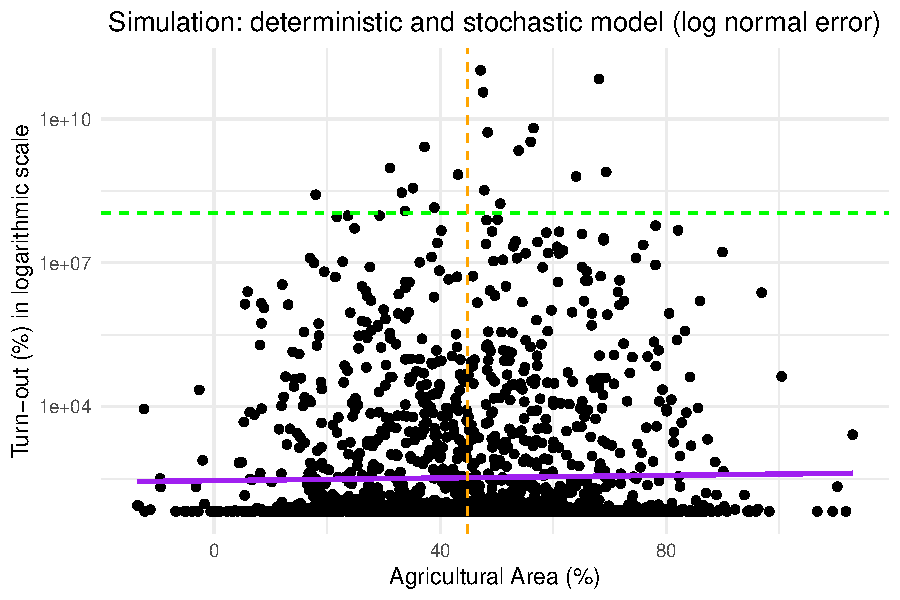
\includegraphics{_main_files/figure-latex/unnamed-chunk-61-1.pdf}

\begin{enumerate}
\def\labelenumi{\arabic{enumi}.}
\setcounter{enumi}{1}
\tightlist
\item
  Since the political preferences as well as years are defined in discrete values, many values can overlap for the same pair\texttt{(preference,\ age)}. Use the \texttt{ggridges} package to see how do preferences distribute across different age values.
\end{enumerate}

\begin{Shaded}
\begin{Highlighting}[]
\FunctionTok{ggplot}\NormalTok{(selects19, }\FunctionTok{aes}\NormalTok{(}\AttributeTok{x =}\NormalTok{ age, }\AttributeTok{y =} \FunctionTok{as.factor}\NormalTok{(LeftToRight), }\AttributeTok{fill =} \FunctionTok{as.factor}\NormalTok{(LeftToRight))) }\SpecialCharTok{+}
  \FunctionTok{geom\_density\_ridges}\NormalTok{() }\SpecialCharTok{+}
  \FunctionTok{geom\_smooth}\NormalTok{(}\AttributeTok{data =}\NormalTok{ selects19, }\FunctionTok{aes}\NormalTok{(}\AttributeTok{x =}\NormalTok{ age, }\AttributeTok{y =}\NormalTok{ LeftToRight, }\AttributeTok{group =} \DecValTok{1}\NormalTok{), }
              \AttributeTok{method =} \StringTok{"lm"}\NormalTok{, }\AttributeTok{formula =}\NormalTok{ y }\SpecialCharTok{\textasciitilde{}}\NormalTok{ x, }\AttributeTok{color =} \StringTok{"red"}\NormalTok{, }\AttributeTok{se =} \ConstantTok{FALSE}\NormalTok{) }\SpecialCharTok{+}
  \FunctionTok{geom\_hline}\NormalTok{(}\AttributeTok{yintercept =}\NormalTok{ mean\_LeftRight, }\AttributeTok{linetype =} \StringTok{"dashed"}\NormalTok{, }\AttributeTok{color =} \StringTok{"green"}\NormalTok{) }\SpecialCharTok{+}
  \FunctionTok{geom\_vline}\NormalTok{(}\AttributeTok{xintercept =}\NormalTok{ mean\_age, }\AttributeTok{linetype =} \StringTok{"dashed"}\NormalTok{, }\AttributeTok{color =} \StringTok{"orange"}\NormalTok{) }\SpecialCharTok{+}
  \FunctionTok{scale\_fill\_viridis\_d}\NormalTok{() }\SpecialCharTok{+}
  \FunctionTok{theme\_minimal}\NormalTok{() }\SpecialCharTok{+}
  \FunctionTok{theme}\NormalTok{(}\AttributeTok{legend.position =} \StringTok{"none"}\NormalTok{) }\SpecialCharTok{+}
  \FunctionTok{theme}\NormalTok{(}\AttributeTok{plot.title =} \FunctionTok{element\_text}\NormalTok{(}\AttributeTok{hjust =} \FloatTok{0.5}\NormalTok{)) }\SpecialCharTok{+}
  \FunctionTok{labs}\NormalTok{(}\AttributeTok{x =} \StringTok{"Age (years)"}\NormalTok{,}
       \AttributeTok{y =} \StringTok{"Political Preferences (left to right)"}\NormalTok{,}
       \AttributeTok{title =} \StringTok{"Political preferences by age level"}\NormalTok{,}
       \AttributeTok{fill =} \StringTok{"factor(LeftToRight)"}\NormalTok{)}
\end{Highlighting}
\end{Shaded}

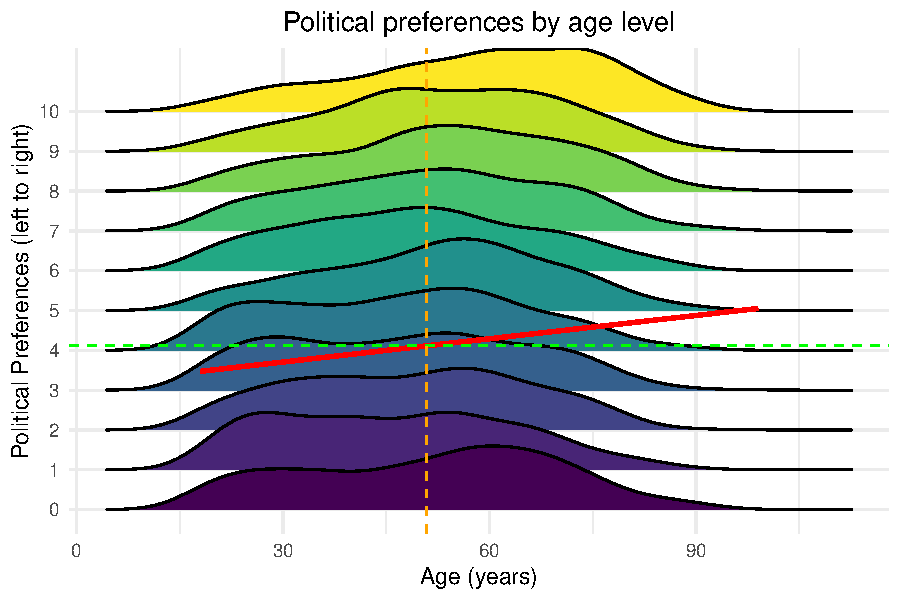
\includegraphics{_main_files/figure-latex/unnamed-chunk-62-1.pdf}

\begin{enumerate}
\def\labelenumi{\arabic{enumi}.}
\setcounter{enumi}{2}
\tightlist
\item
  Regress the political preferences on age. As we learnt in the exercises from last week, the regression with intercept fits data better in most cases: act accordingly. Report and interpret the parameters. Graph some of the main components of the regression output.
\end{enumerate}

Write the regression here.

\begin{Shaded}
\begin{Highlighting}[]
\CommentTok{\#regression}
\NormalTok{result }\OtherTok{\textless{}{-}} \FunctionTok{lm}\NormalTok{(LeftToRight }\SpecialCharTok{\textasciitilde{}}\NormalTok{ age, }\AttributeTok{data =}\NormalTok{ selects19)}
\FunctionTok{summary}\NormalTok{(result)}
\end{Highlighting}
\end{Shaded}

\begin{verbatim}
## 
## Call:
## lm(formula = LeftToRight ~ age, data = selects19)
## 
## Residuals:
##     Min      1Q  Median      3Q     Max 
## -5.9150 -2.0380 -0.0186  2.1958  5.5271 
## 
## Coefficients:
##             Estimate Std. Error t value Pr(>|t|)    
## (Intercept) 4.122055   0.106375  38.750   <2e-16 ***
## age         0.019489   0.001979   9.846   <2e-16 ***
## ---
## Signif. codes:  0 '***' 0.001 '**' 0.01 '*' 0.05 '.' 0.1 ' ' 1
## 
## Residual standard error: 2.649 on 5905 degrees of freedom
## Multiple R-squared:  0.01615,    Adjusted R-squared:  0.01598 
## F-statistic: 96.94 on 1 and 5905 DF,  p-value: < 2.2e-16
\end{verbatim}

Report and interpret the parameters here.

\begin{Shaded}
\begin{Highlighting}[]
\NormalTok{coeffs}\OtherTok{\textless{}{-}} \FunctionTok{coef}\NormalTok{(result)}
\FunctionTok{cat}\NormalTok{(}\StringTok{\textquotesingle{}The beta value for\textquotesingle{}}\NormalTok{, }\FunctionTok{names}\NormalTok{(coeffs[}\DecValTok{1}\NormalTok{]), }\StringTok{\textquotesingle{} is \textquotesingle{}}\NormalTok{, }\FunctionTok{round}\NormalTok{(}\FunctionTok{unname}\NormalTok{(coeffs[}\DecValTok{1}\NormalTok{]), }\AttributeTok{digits =} \DecValTok{2}\NormalTok{), }\StringTok{\textquotesingle{} and for \textquotesingle{}}\NormalTok{, }\FunctionTok{names}\NormalTok{(coeffs[}\DecValTok{2}\NormalTok{]), }\StringTok{\textquotesingle{} is \textquotesingle{}}\NormalTok{, }\FunctionTok{round}\NormalTok{(}\FunctionTok{unname}\NormalTok{(coeffs[}\DecValTok{2}\NormalTok{]), }\AttributeTok{digits =} \DecValTok{2}\NormalTok{), }\StringTok{\textquotesingle{}. }\SpecialCharTok{\textbackslash{}n\textbackslash{}n}\StringTok{It means that, given our model, an increase of one year in age across the Swiss citizens is associated with an average increase in the LeftToRight self{-}declared scale of \textquotesingle{}}\NormalTok{, }\FunctionTok{round}\NormalTok{(}\FunctionTok{unname}\NormalTok{(coeffs[}\DecValTok{2}\NormalTok{]), }\AttributeTok{digits =} \DecValTok{2}\NormalTok{), }\StringTok{\textquotesingle{} }\SpecialCharTok{\textbackslash{}\textquotesingle{}}\StringTok{ideological units}\SpecialCharTok{\textbackslash{}\textquotesingle{}}\StringTok{. Likewise, newborns can be expected to have an average ideological value of \textquotesingle{}}\NormalTok{,}\FunctionTok{round}\NormalTok{(}\FunctionTok{unname}\NormalTok{(coeffs[}\DecValTok{1}\NormalTok{]), }\AttributeTok{digits =} \DecValTok{2}\NormalTok{),}\StringTok{\textquotesingle{}, while 100 year old citizens can be expected to have an average ideological value of.\textquotesingle{}}\NormalTok{, }\FunctionTok{round}\NormalTok{(}\FunctionTok{unname}\NormalTok{(coeffs[}\DecValTok{1}\NormalTok{]), }\AttributeTok{digits =} \DecValTok{2}\NormalTok{)}\SpecialCharTok{+}\FunctionTok{round}\NormalTok{(}\FunctionTok{unname}\NormalTok{(coeffs[}\DecValTok{2}\NormalTok{]), }\AttributeTok{digits =} \DecValTok{2}\NormalTok{)}\SpecialCharTok{*}\DecValTok{100}\NormalTok{)}
\end{Highlighting}
\end{Shaded}

\begin{verbatim}
## The beta value for (Intercept)  is  4.12  and for  age  is  0.02 . 
## 
## It means that, given our model, an increase of one year in age across the Swiss citizens is associated with an average increase in the LeftToRight self-declared scale of  0.02  'ideological units'. Likewise, newborns can be expected to have an average ideological value of  4.12 , while 100 year old citizens can be expected to have an average ideological value of. 6.12
\end{verbatim}

Graph some of the main components of the regression output here.

\begin{Shaded}
\begin{Highlighting}[]
\FunctionTok{ggplot}\NormalTok{(selects19, }\FunctionTok{aes}\NormalTok{(}\AttributeTok{x =}\NormalTok{ age, }\AttributeTok{y =}\NormalTok{ LeftToRight)) }\SpecialCharTok{+}  \CommentTok{\# Removed selects19$ from aes(), not necessary}
  \FunctionTok{geom\_point}\NormalTok{(}\AttributeTok{size =} \FloatTok{0.001}\NormalTok{) }\SpecialCharTok{+}
  \FunctionTok{geom\_abline}\NormalTok{(}\AttributeTok{intercept =} \FunctionTok{unname}\NormalTok{(coeffs[}\DecValTok{1}\NormalTok{]),}
              \AttributeTok{slope =} \DecValTok{0}\NormalTok{, }\AttributeTok{color =} \StringTok{"gray"}\NormalTok{, }\AttributeTok{size =} \DecValTok{1}\NormalTok{) }\SpecialCharTok{+}
  \FunctionTok{geom\_text}\NormalTok{(}\FunctionTok{aes}\NormalTok{(}\AttributeTok{label =} \StringTok{"Newborn"}\NormalTok{,}
                \AttributeTok{x =} \FunctionTok{max}\NormalTok{(selects19}\SpecialCharTok{$}\NormalTok{age)}\SpecialCharTok{+}\DecValTok{10}\NormalTok{,}
                \AttributeTok{y =} \FloatTok{0.2}\SpecialCharTok{+}\FunctionTok{unname}\NormalTok{(coeffs[}\DecValTok{1}\NormalTok{])),}
                \AttributeTok{hjust =} \DecValTok{1}\NormalTok{, }\AttributeTok{vjust =} \DecValTok{0}\NormalTok{, }\AttributeTok{color =} \StringTok{"gray"}\NormalTok{)}\SpecialCharTok{+} 

  \FunctionTok{geom\_abline}\NormalTok{(}\AttributeTok{intercept =} \FunctionTok{unname}\NormalTok{(coeffs[}\DecValTok{1}\NormalTok{]),}
              \AttributeTok{slope =} \FunctionTok{unname}\NormalTok{(coeffs[}\DecValTok{2}\NormalTok{]), }\AttributeTok{color =} \StringTok{"red"}\NormalTok{, }\AttributeTok{size =} \DecValTok{1}\NormalTok{) }\SpecialCharTok{+}
  \FunctionTok{geom\_text}\NormalTok{(}\FunctionTok{aes}\NormalTok{(}\AttributeTok{label =} \StringTok{"Average individual over time"}\NormalTok{,}
                \AttributeTok{x =} \FunctionTok{max}\NormalTok{(selects19}\SpecialCharTok{$}\NormalTok{age)}\SpecialCharTok{+}\DecValTok{10}\NormalTok{,}
                \AttributeTok{y =} \FloatTok{0.4}\SpecialCharTok{+}\FunctionTok{unname}\NormalTok{(coeffs[}\DecValTok{1}\NormalTok{]) }\SpecialCharTok{+} \FunctionTok{unname}\NormalTok{(coeffs[}\DecValTok{2}\NormalTok{]) }\SpecialCharTok{*} \FunctionTok{max}\NormalTok{(selects19}\SpecialCharTok{$}\NormalTok{age)),}
                \AttributeTok{hjust =} \DecValTok{1}\NormalTok{, }\AttributeTok{vjust =} \DecValTok{0}\NormalTok{, }\AttributeTok{color =} \StringTok{"red"}\NormalTok{) }\SpecialCharTok{+}

  \FunctionTok{theme\_minimal}\NormalTok{() }\SpecialCharTok{+}
  \FunctionTok{theme}\NormalTok{(}\AttributeTok{plot.title =} \FunctionTok{element\_text}\NormalTok{(}\AttributeTok{hjust =} \FloatTok{0.5}\NormalTok{)) }\SpecialCharTok{+}
  \FunctionTok{labs}\NormalTok{(}
    \AttributeTok{x =} \StringTok{"Age (years)"}\NormalTok{,}
    \AttributeTok{y =} \StringTok{"Political Preferences (left to right)"}\NormalTok{,}
    \AttributeTok{title =} \StringTok{"Lines Using Parameters from Regression"}
\NormalTok{  )}
\end{Highlighting}
\end{Shaded}

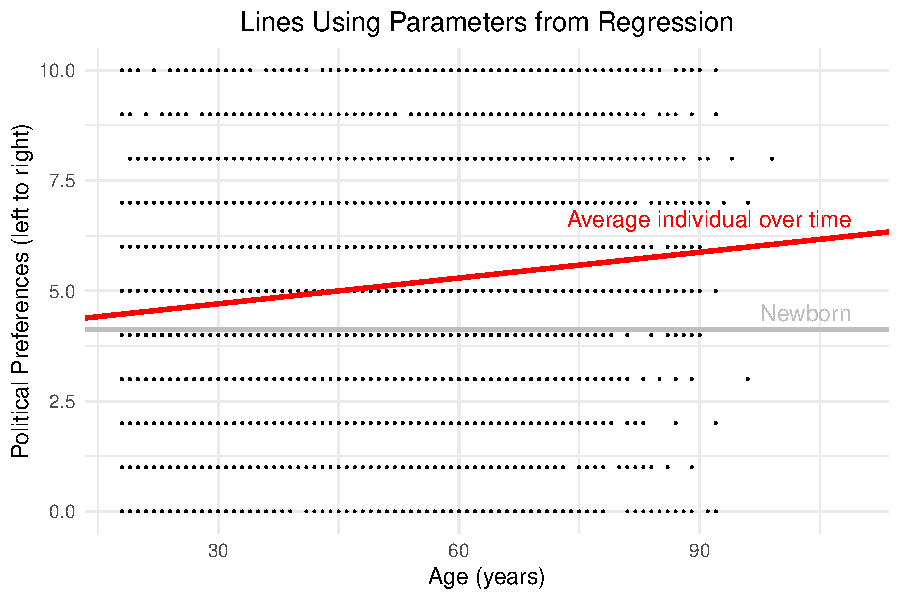
\includegraphics{_main_files/figure-latex/unnamed-chunk-65-1.pdf}

\begin{enumerate}
\def\labelenumi{\arabic{enumi}.}
\setcounter{enumi}{3}
\tightlist
\item
  Now add the regressor \texttt{Sex} and do the same as in the previous point.
  Write the regression here.
\end{enumerate}

\begin{Shaded}
\begin{Highlighting}[]
\CommentTok{\#regression}
\NormalTok{result }\OtherTok{\textless{}{-}} \FunctionTok{lm}\NormalTok{(LeftToRight }\SpecialCharTok{\textasciitilde{}}\NormalTok{ age }\SpecialCharTok{+}\NormalTok{ Sex, }\AttributeTok{data =}\NormalTok{ selects19)}
\FunctionTok{summary}\NormalTok{(result)}
\end{Highlighting}
\end{Shaded}

\begin{verbatim}
## 
## Call:
## lm(formula = LeftToRight ~ age + Sex, data = selects19)
## 
## Residuals:
##     Min      1Q  Median      3Q     Max 
## -6.2108 -1.9784  0.0954  2.1145  5.8236 
## 
## Coefficients:
##             Estimate Std. Error t value Pr(>|t|)    
## (Intercept) 3.840287   0.109636  35.028   <2e-16 ***
## age         0.018672   0.001966   9.496   <2e-16 ***
## SexMale     0.652678   0.068477   9.531   <2e-16 ***
## ---
## Signif. codes:  0 '***' 0.001 '**' 0.01 '*' 0.05 '.' 0.1 ' ' 1
## 
## Residual standard error: 2.629 on 5904 degrees of freedom
## Multiple R-squared:  0.03106,    Adjusted R-squared:  0.03073 
## F-statistic: 94.63 on 2 and 5904 DF,  p-value: < 2.2e-16
\end{verbatim}

Report and interpret the parameters here.

\begin{Shaded}
\begin{Highlighting}[]
\NormalTok{coeffs}\OtherTok{\textless{}{-}} \FunctionTok{coef}\NormalTok{(result)}
\FunctionTok{cat}\NormalTok{(}\StringTok{\textquotesingle{}The beta value for\textquotesingle{}}\NormalTok{, }\FunctionTok{names}\NormalTok{(coeffs[}\DecValTok{1}\NormalTok{]), }\StringTok{\textquotesingle{} is \textquotesingle{}}\NormalTok{, }\FunctionTok{round}\NormalTok{(}\FunctionTok{unname}\NormalTok{(coeffs[}\DecValTok{1}\NormalTok{]), }\AttributeTok{digits =} \DecValTok{2}\NormalTok{), }\StringTok{\textquotesingle{} for \textquotesingle{}}\NormalTok{, }\FunctionTok{names}\NormalTok{(coeffs[}\DecValTok{2}\NormalTok{]), }\StringTok{\textquotesingle{} is \textquotesingle{}}\NormalTok{, }\FunctionTok{round}\NormalTok{(}\FunctionTok{unname}\NormalTok{(coeffs[}\DecValTok{2}\NormalTok{]), }\AttributeTok{digits =} \DecValTok{2}\NormalTok{), }\StringTok{\textquotesingle{} and for \textquotesingle{}}\NormalTok{, }\FunctionTok{names}\NormalTok{(coeffs[}\DecValTok{3}\NormalTok{]), }\StringTok{\textquotesingle{} is \textquotesingle{}}\NormalTok{, }\FunctionTok{round}\NormalTok{(}\FunctionTok{unname}\NormalTok{(coeffs[}\DecValTok{3}\NormalTok{]), }\AttributeTok{digits =} \DecValTok{2}\NormalTok{),}
    
\StringTok{\textquotesingle{}. }\SpecialCharTok{\textbackslash{}n\textbackslash{}n}\StringTok{It means that, given our model,  an increase of one year in age across the Swiss citizens is associated with an average increase in the LeftToRight self{-}declared scale of \textquotesingle{}}\NormalTok{, }\FunctionTok{round}\NormalTok{(}\FunctionTok{unname}\NormalTok{(coeffs[}\DecValTok{2}\NormalTok{]), }\AttributeTok{digits =} \DecValTok{2}\NormalTok{), }\StringTok{\textquotesingle{} }\SpecialCharTok{\textbackslash{}\textquotesingle{}}\StringTok{ideological units}\SpecialCharTok{\textbackslash{}\textquotesingle{}}\StringTok{. Likewise, newborns can be expected to have an average ideological value of \textquotesingle{}}\NormalTok{,}\FunctionTok{round}\NormalTok{(}\FunctionTok{unname}\NormalTok{(coeffs[}\DecValTok{1}\NormalTok{]), }\AttributeTok{digits =} \DecValTok{2}\NormalTok{),}\StringTok{\textquotesingle{}, while 100 year old female citizens can be expected to have an average ideological value of.\textquotesingle{}}\NormalTok{, }\FunctionTok{round}\NormalTok{(}\FunctionTok{unname}\NormalTok{(coeffs[}\DecValTok{1}\NormalTok{]), }\AttributeTok{digits =} \DecValTok{2}\NormalTok{)}\SpecialCharTok{+}\FunctionTok{round}\NormalTok{(}\FunctionTok{unname}\NormalTok{(coeffs[}\DecValTok{2}\NormalTok{]), }\AttributeTok{digits =} \DecValTok{2}\NormalTok{)}\SpecialCharTok{*}\DecValTok{100}\NormalTok{, }\StringTok{\textquotesingle{}. Similarly, for each of those scenarios, should the individual be a male, it can be expected to have an average of \textquotesingle{}}\NormalTok{, }\FunctionTok{round}\NormalTok{(}\FunctionTok{unname}\NormalTok{(coeffs[}\DecValTok{3}\NormalTok{]), }\AttributeTok{digits =} \DecValTok{2}\NormalTok{), }\StringTok{\textquotesingle{} ideological units higher than a female individual under the same statistical circumstances.\textquotesingle{}}\NormalTok{)}
\end{Highlighting}
\end{Shaded}

\begin{verbatim}
## The beta value for (Intercept)  is  3.84  for  age  is  0.02  and for  SexMale  is  0.65 . 
## 
## It means that, given our model,  an increase of one year in age across the Swiss citizens is associated with an average increase in the LeftToRight self-declared scale of  0.02  'ideological units'. Likewise, newborns can be expected to have an average ideological value of  3.84 , while 100 year old female citizens can be expected to have an average ideological value of. 5.84 . Similarly, for each of those scenarios, should the individual be a male, it can be expected to have an average of  0.65  ideological units higher than a female individual under the same statistical circumstances.
\end{verbatim}

Graph some of the main components of the regression output here.

\begin{Shaded}
\begin{Highlighting}[]
\FunctionTok{ggplot}\NormalTok{(selects19, }\FunctionTok{aes}\NormalTok{(}\AttributeTok{x =}\NormalTok{ age, }\AttributeTok{y =}\NormalTok{ LeftToRight)) }\SpecialCharTok{+}  \CommentTok{\# Removed selects19$ from aes(), not necessary}
  \FunctionTok{geom\_point}\NormalTok{(}\AttributeTok{size =} \FloatTok{0.001}\NormalTok{) }\SpecialCharTok{+}
  \FunctionTok{geom\_abline}\NormalTok{(}\AttributeTok{intercept =} \FunctionTok{unname}\NormalTok{(coeffs[}\DecValTok{1}\NormalTok{]),}
              \AttributeTok{slope =} \DecValTok{0}\NormalTok{, }\AttributeTok{color =} \StringTok{"gray"}\NormalTok{, }\AttributeTok{size =} \DecValTok{1}\NormalTok{) }\SpecialCharTok{+}
  \FunctionTok{geom\_text}\NormalTok{(}\FunctionTok{aes}\NormalTok{(}\AttributeTok{label =} \StringTok{"Newborn female"}\NormalTok{,}
                \AttributeTok{x =} \FunctionTok{max}\NormalTok{(selects19}\SpecialCharTok{$}\NormalTok{age)}\SpecialCharTok{+}\DecValTok{10}\NormalTok{,}
                \AttributeTok{y =} \FloatTok{0.2}\SpecialCharTok{+}\FunctionTok{unname}\NormalTok{(coeffs[}\DecValTok{1}\NormalTok{])),}
                \AttributeTok{hjust =} \DecValTok{1}\NormalTok{, }\AttributeTok{vjust =} \DecValTok{0}\NormalTok{, }\AttributeTok{color =} \StringTok{"gray"}\NormalTok{)}\SpecialCharTok{+} 

  \FunctionTok{geom\_abline}\NormalTok{(}\AttributeTok{intercept =} \FunctionTok{unname}\NormalTok{(coeffs[}\DecValTok{1}\NormalTok{]),}
              \AttributeTok{slope =} \FunctionTok{unname}\NormalTok{(coeffs[}\DecValTok{2}\NormalTok{]), }\AttributeTok{color =} \StringTok{"red"}\NormalTok{, }\AttributeTok{size =} \DecValTok{1}\NormalTok{) }\SpecialCharTok{+}
  \FunctionTok{geom\_text}\NormalTok{(}\FunctionTok{aes}\NormalTok{(}\AttributeTok{label =} \StringTok{"Female over time"}\NormalTok{,}
                \AttributeTok{x =} \FunctionTok{max}\NormalTok{(selects19}\SpecialCharTok{$}\NormalTok{age)}\SpecialCharTok{+}\DecValTok{10}\NormalTok{,}
                \AttributeTok{y =} \SpecialCharTok{{-}}\FloatTok{0.8}\SpecialCharTok{+}\FunctionTok{unname}\NormalTok{(coeffs[}\DecValTok{1}\NormalTok{]) }\SpecialCharTok{+} \FunctionTok{unname}\NormalTok{(coeffs[}\DecValTok{2}\NormalTok{]) }\SpecialCharTok{*} \FunctionTok{max}\NormalTok{(selects19}\SpecialCharTok{$}\NormalTok{age)),}
                \AttributeTok{hjust =} \DecValTok{1}\NormalTok{, }\AttributeTok{vjust =} \DecValTok{0}\NormalTok{, }\AttributeTok{color =} \StringTok{"red"}\NormalTok{) }\SpecialCharTok{+}

  \FunctionTok{geom\_abline}\NormalTok{(}\AttributeTok{intercept =} \FunctionTok{unname}\NormalTok{(coeffs[}\DecValTok{1}\NormalTok{])}\SpecialCharTok{+}\FunctionTok{unname}\NormalTok{(coeffs[}\DecValTok{3}\NormalTok{]),}
              \AttributeTok{slope =} \FunctionTok{unname}\NormalTok{(coeffs[}\DecValTok{2}\NormalTok{]), }\AttributeTok{color =} \StringTok{"orange"}\NormalTok{, }\AttributeTok{size =} \DecValTok{1}\NormalTok{) }\SpecialCharTok{+}
  \FunctionTok{geom\_text}\NormalTok{(}\FunctionTok{aes}\NormalTok{(}\AttributeTok{label =} \StringTok{"Male over time (newborn bonus)"}\NormalTok{,}
                \AttributeTok{x =} \FunctionTok{max}\NormalTok{(selects19}\SpecialCharTok{$}\NormalTok{age)}\SpecialCharTok{+}\DecValTok{10}\NormalTok{,}
                \AttributeTok{y =} \FloatTok{0.6}\SpecialCharTok{+}\FunctionTok{unname}\NormalTok{(coeffs[}\DecValTok{1}\NormalTok{])}\SpecialCharTok{+}\FunctionTok{unname}\NormalTok{(coeffs[}\DecValTok{3}\NormalTok{]) }\SpecialCharTok{+} \FunctionTok{unname}\NormalTok{(coeffs[}\DecValTok{2}\NormalTok{]) }\SpecialCharTok{*} \FunctionTok{max}\NormalTok{(selects19}\SpecialCharTok{$}\NormalTok{age)}\SpecialCharTok{+}\FloatTok{0.2}\NormalTok{),}
                \AttributeTok{hjust =} \DecValTok{1}\NormalTok{, }\AttributeTok{vjust =} \DecValTok{0}\NormalTok{, }\AttributeTok{color =} \StringTok{"orange"}\NormalTok{) }\SpecialCharTok{+}

  \FunctionTok{theme\_minimal}\NormalTok{() }\SpecialCharTok{+}
  \FunctionTok{theme}\NormalTok{(}\AttributeTok{plot.title =} \FunctionTok{element\_text}\NormalTok{(}\AttributeTok{hjust =} \FloatTok{0.5}\NormalTok{)) }\SpecialCharTok{+}
  \FunctionTok{labs}\NormalTok{(}
    \AttributeTok{x =} \StringTok{"Age (years)"}\NormalTok{,}
    \AttributeTok{y =} \StringTok{"Political Preferences (left to right)"}\NormalTok{,}
    \AttributeTok{title =} \StringTok{"Lines Using Parameters from Regression"}
\NormalTok{  )}
\end{Highlighting}
\end{Shaded}

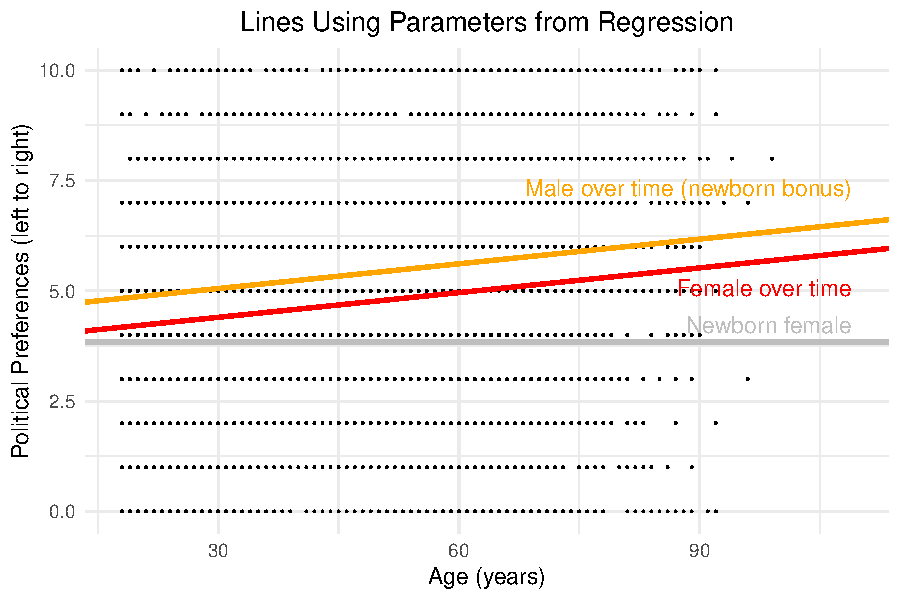
\includegraphics{_main_files/figure-latex/unnamed-chunk-68-1.pdf}

\begin{enumerate}
\def\labelenumi{\arabic{enumi}.}
\setcounter{enumi}{4}
\tightlist
\item
  You now remember that average preferences can change not only across age and sex independently, but simultaneously: i.e., the average preferences across individuals in a same sex can change at different rates over time as well as begin from different points. Add the interaction \texttt{Age} and \texttt{Sex} and do the same as in the previous point.
\end{enumerate}

Write the regression here.

\begin{Shaded}
\begin{Highlighting}[]
\CommentTok{\#regression}
\NormalTok{result }\OtherTok{\textless{}{-}} \FunctionTok{lm}\NormalTok{(LeftToRight }\SpecialCharTok{\textasciitilde{}}\NormalTok{ age }\SpecialCharTok{*}\NormalTok{ Sex, }\AttributeTok{data =}\NormalTok{ selects19)}
\FunctionTok{summary}\NormalTok{(result)}
\end{Highlighting}
\end{Shaded}

\begin{verbatim}
## 
## Call:
## lm(formula = LeftToRight ~ age * Sex, data = selects19)
## 
## Residuals:
##     Min      1Q  Median      3Q     Max 
## -5.9332 -2.0641  0.0372  2.1848  6.0372 
## 
## Coefficients:
##              Estimate Std. Error t value Pr(>|t|)    
## (Intercept)  3.506922   0.146203  23.987  < 2e-16 ***
## age          0.025327   0.002756   9.189  < 2e-16 ***
## SexMale      1.340734   0.211254   6.347 2.37e-10 ***
## age:SexMale -0.013528   0.003930  -3.443  0.00058 ***
## ---
## Signif. codes:  0 '***' 0.001 '**' 0.01 '*' 0.05 '.' 0.1 ' ' 1
## 
## Residual standard error: 2.626 on 5903 degrees of freedom
## Multiple R-squared:  0.033,  Adjusted R-squared:  0.03251 
## F-statistic: 67.15 on 3 and 5903 DF,  p-value: < 2.2e-16
\end{verbatim}

Report and interpret the parameters here.

\begin{Shaded}
\begin{Highlighting}[]
\NormalTok{coeffs}\OtherTok{\textless{}{-}} \FunctionTok{coef}\NormalTok{(result)}
\FunctionTok{cat}\NormalTok{(}\StringTok{\textquotesingle{}The beta value for\textquotesingle{}}\NormalTok{, }\FunctionTok{names}\NormalTok{(coeffs[}\DecValTok{1}\NormalTok{]), }\StringTok{\textquotesingle{} is \textquotesingle{}}\NormalTok{, }\FunctionTok{round}\NormalTok{(}\FunctionTok{unname}\NormalTok{(coeffs[}\DecValTok{1}\NormalTok{]), }\AttributeTok{digits =} \DecValTok{2}\NormalTok{), }\StringTok{\textquotesingle{} for \textquotesingle{}}\NormalTok{, }\FunctionTok{names}\NormalTok{(coeffs[}\DecValTok{2}\NormalTok{]), }\StringTok{\textquotesingle{} is \textquotesingle{}}\NormalTok{, }\FunctionTok{round}\NormalTok{(}\FunctionTok{unname}\NormalTok{(coeffs[}\DecValTok{2}\NormalTok{]), }\AttributeTok{digits =} \DecValTok{2}\NormalTok{), }\StringTok{\textquotesingle{} for \textquotesingle{}}\NormalTok{, }\FunctionTok{names}\NormalTok{(coeffs[}\DecValTok{3}\NormalTok{]), }\StringTok{\textquotesingle{} is \textquotesingle{}}\NormalTok{, }\FunctionTok{round}\NormalTok{(}\FunctionTok{unname}\NormalTok{(coeffs[}\DecValTok{3}\NormalTok{]), }\AttributeTok{digits =} \DecValTok{2}\NormalTok{),}\StringTok{\textquotesingle{} and for \textquotesingle{}}\NormalTok{, }\FunctionTok{names}\NormalTok{(coeffs[}\DecValTok{4}\NormalTok{]), }\StringTok{\textquotesingle{} is \textquotesingle{}}\NormalTok{, }\FunctionTok{round}\NormalTok{(}\FunctionTok{unname}\NormalTok{(coeffs[}\DecValTok{4}\NormalTok{]), }\AttributeTok{digits =} \DecValTok{2}\NormalTok{),}
    
\StringTok{\textquotesingle{}. }\SpecialCharTok{\textbackslash{}n\textbackslash{}n}\StringTok{It means that, given our model,  an increase of one year in age across the female Swiss citizens is associated with an average increase in the LeftToRight self{-}declared scale of \textquotesingle{}}\NormalTok{, }\FunctionTok{round}\NormalTok{(}\FunctionTok{unname}\NormalTok{(coeffs[}\DecValTok{2}\NormalTok{]), }\AttributeTok{digits =} \DecValTok{2}\NormalTok{), }\StringTok{\textquotesingle{} }\SpecialCharTok{\textbackslash{}\textquotesingle{}}\StringTok{ideological units}\SpecialCharTok{\textbackslash{}\textquotesingle{}}\StringTok{. Likewise, female newborns can be expected to have an average ideological value of \textquotesingle{}}\NormalTok{,}\FunctionTok{round}\NormalTok{(}\FunctionTok{unname}\NormalTok{(coeffs[}\DecValTok{1}\NormalTok{]), }\AttributeTok{digits =} \DecValTok{2}\NormalTok{),}\StringTok{\textquotesingle{}, while 100 year old female citizens can be expected to have an average ideological value of.\textquotesingle{}}\NormalTok{, }\FunctionTok{round}\NormalTok{(}\FunctionTok{unname}\NormalTok{(coeffs[}\DecValTok{1}\NormalTok{]), }\AttributeTok{digits =} \DecValTok{2}\NormalTok{)}\SpecialCharTok{+}\FunctionTok{round}\NormalTok{(}\FunctionTok{unname}\NormalTok{(coeffs[}\DecValTok{2}\NormalTok{]), }\AttributeTok{digits =} \DecValTok{2}\NormalTok{)}\SpecialCharTok{*}\DecValTok{100}\NormalTok{, }\StringTok{\textquotesingle{}. }\SpecialCharTok{\textbackslash{}n\textbackslash{}n}\StringTok{Similarly, for each of those scenarios, should the individual be a male, it can be expected to have an average of \textquotesingle{}}\NormalTok{, }\FunctionTok{round}\NormalTok{(}\FunctionTok{unname}\NormalTok{(coeffs[}\DecValTok{3}\NormalTok{]), }\AttributeTok{digits =} \DecValTok{2}\NormalTok{), }\StringTok{\textquotesingle{} ideological units higher (i.e., self declare more right leaning) than a female individual under the same statistical circumstances. Finally, the rate at which right leaning prefferences increase over time is \textquotesingle{}}\NormalTok{, }\FunctionTok{round}\NormalTok{(}\FunctionTok{unname}\NormalTok{(coeffs[}\DecValTok{4}\NormalTok{]), }\AttributeTok{digits =} \DecValTok{2}\NormalTok{)}\SpecialCharTok{*{-}}\DecValTok{1}\NormalTok{, }\StringTok{\textquotesingle{} lower than a female in the same statistical circumstances. Therefore, a 100 year old male can be expected to have an political preference of \textquotesingle{}}\NormalTok{, }\FunctionTok{round}\NormalTok{(}\FunctionTok{unname}\NormalTok{(coeffs[}\DecValTok{1}\NormalTok{]), }\AttributeTok{digits =} \DecValTok{2}\NormalTok{)}\SpecialCharTok{+}\FunctionTok{round}\NormalTok{(}\FunctionTok{unname}\NormalTok{(coeffs[}\DecValTok{2}\NormalTok{]), }\AttributeTok{digits =} \DecValTok{2}\NormalTok{)}\SpecialCharTok{*}\DecValTok{100}\SpecialCharTok{+}\FunctionTok{round}\NormalTok{(}\FunctionTok{unname}\NormalTok{(coeffs[}\DecValTok{3}\NormalTok{]), }\AttributeTok{digits =} \DecValTok{2}\NormalTok{)}\SpecialCharTok{+}\FunctionTok{round}\NormalTok{(}\FunctionTok{unname}\NormalTok{(coeffs[}\DecValTok{4}\NormalTok{]), }\AttributeTok{digits =} \DecValTok{2}\NormalTok{)}\SpecialCharTok{*}\DecValTok{100}\NormalTok{)}
\end{Highlighting}
\end{Shaded}

\begin{verbatim}
## The beta value for (Intercept)  is  3.51  for  age  is  0.03  for  SexMale  is  1.34  and for  age:SexMale  is  -0.01 . 
## 
## It means that, given our model,  an increase of one year in age across the female Swiss citizens is associated with an average increase in the LeftToRight self-declared scale of  0.03  'ideological units'. Likewise, female newborns can be expected to have an average ideological value of  3.51 , while 100 year old female citizens can be expected to have an average ideological value of. 6.51 . 
## 
## Similarly, for each of those scenarios, should the individual be a male, it can be expected to have an average of  1.34  ideological units higher (i.e., self declare more right leaning) than a female individual under the same statistical circumstances. Finally, the rate at which right leaning prefferences increase over time is  0.01  lower than a female in the same statistical circumstances. Therefore, a 100 year old male can be expected to have an political preference of  6.85
\end{verbatim}

Graph some of the main components of the regression output here.

\begin{Shaded}
\begin{Highlighting}[]
\FunctionTok{ggplot}\NormalTok{(selects19, }\FunctionTok{aes}\NormalTok{(}\AttributeTok{x =}\NormalTok{ age, }\AttributeTok{y =}\NormalTok{ LeftToRight)) }\SpecialCharTok{+}
  \FunctionTok{geom\_point}\NormalTok{(}\AttributeTok{size =} \DecValTok{0}\NormalTok{) }\SpecialCharTok{+}
  \FunctionTok{geom\_abline}\NormalTok{(}\AttributeTok{intercept =} \FunctionTok{unname}\NormalTok{(coeffs[}\DecValTok{1}\NormalTok{]),}
              \AttributeTok{slope =} \DecValTok{0}\NormalTok{, }\AttributeTok{color =} \StringTok{"gray"}\NormalTok{, }\AttributeTok{size =} \DecValTok{1}\NormalTok{) }\SpecialCharTok{+}
  \FunctionTok{geom\_text}\NormalTok{(}\FunctionTok{aes}\NormalTok{(}\AttributeTok{label =} \StringTok{"Newborn female"}\NormalTok{,}
                \AttributeTok{x =} \FunctionTok{max}\NormalTok{(selects19}\SpecialCharTok{$}\NormalTok{age)}\SpecialCharTok{+}\DecValTok{10}\NormalTok{,}
                \AttributeTok{y =} \SpecialCharTok{{-}}\FloatTok{0.5}\SpecialCharTok{+}\FunctionTok{unname}\NormalTok{(coeffs[}\DecValTok{1}\NormalTok{])),}
                \AttributeTok{hjust =} \DecValTok{1}\NormalTok{, }\AttributeTok{vjust =} \DecValTok{0}\NormalTok{, }\AttributeTok{color =} \StringTok{"gray"}\NormalTok{)}\SpecialCharTok{+} 

  \FunctionTok{geom\_abline}\NormalTok{(}\AttributeTok{intercept =} \FunctionTok{unname}\NormalTok{(coeffs[}\DecValTok{1}\NormalTok{]),}
              \AttributeTok{slope =} \FunctionTok{unname}\NormalTok{(coeffs[}\DecValTok{2}\NormalTok{]), }\AttributeTok{color =} \StringTok{"red"}\NormalTok{, }\AttributeTok{size =} \DecValTok{1}\NormalTok{) }\SpecialCharTok{+}
  \FunctionTok{geom\_text}\NormalTok{(}\FunctionTok{aes}\NormalTok{(}\AttributeTok{label =} \StringTok{"Female over time"}\NormalTok{,}
                \AttributeTok{x =} \FunctionTok{max}\NormalTok{(selects19}\SpecialCharTok{$}\NormalTok{age)}\SpecialCharTok{+}\DecValTok{10}\NormalTok{,}
                \AttributeTok{y =} \SpecialCharTok{{-}}\FloatTok{0.8}\SpecialCharTok{+}\FunctionTok{unname}\NormalTok{(coeffs[}\DecValTok{1}\NormalTok{]) }\SpecialCharTok{+} \FunctionTok{unname}\NormalTok{(coeffs[}\DecValTok{2}\NormalTok{]) }\SpecialCharTok{*} \FunctionTok{max}\NormalTok{(selects19}\SpecialCharTok{$}\NormalTok{age)),}
                \AttributeTok{hjust =} \DecValTok{1}\NormalTok{, }\AttributeTok{vjust =} \DecValTok{0}\NormalTok{, }\AttributeTok{color =} \StringTok{"red"}\NormalTok{) }\SpecialCharTok{+}

  \FunctionTok{geom\_abline}\NormalTok{(}\AttributeTok{intercept =} \FunctionTok{unname}\NormalTok{(coeffs[}\DecValTok{1}\NormalTok{])}\SpecialCharTok{+}\FunctionTok{unname}\NormalTok{(coeffs[}\DecValTok{3}\NormalTok{]),}
              \AttributeTok{slope =} \FunctionTok{unname}\NormalTok{(coeffs[}\DecValTok{2}\NormalTok{])}\SpecialCharTok{+}\FunctionTok{unname}\NormalTok{(coeffs[}\DecValTok{4}\NormalTok{]), }\AttributeTok{color =} \StringTok{"orange"}\NormalTok{, }\AttributeTok{size =} \DecValTok{1}\NormalTok{) }\SpecialCharTok{+}
  \FunctionTok{geom\_text}\NormalTok{(}\FunctionTok{aes}\NormalTok{(}\AttributeTok{label =} \StringTok{"Male over time (newborn bonus+Δslope)"}\NormalTok{,}
                \AttributeTok{x =} \FunctionTok{max}\NormalTok{(selects19}\SpecialCharTok{$}\NormalTok{age)}\SpecialCharTok{+}\DecValTok{10}\NormalTok{,}
                \AttributeTok{y =} \FloatTok{0.45}\SpecialCharTok{+}\FunctionTok{unname}\NormalTok{(coeffs[}\DecValTok{1}\NormalTok{])}\SpecialCharTok{+}\FunctionTok{unname}\NormalTok{(coeffs[}\DecValTok{3}\NormalTok{]) }\SpecialCharTok{+}\NormalTok{ (}\FunctionTok{unname}\NormalTok{(coeffs[}\DecValTok{2}\NormalTok{])}\SpecialCharTok{+}\FunctionTok{unname}\NormalTok{(coeffs[}\DecValTok{4}\NormalTok{])) }\SpecialCharTok{*} \FunctionTok{max}\NormalTok{(selects19}\SpecialCharTok{$}\NormalTok{age)),}
                \AttributeTok{hjust =} \DecValTok{1}\NormalTok{, }\AttributeTok{vjust =} \DecValTok{0}\NormalTok{, }\AttributeTok{color =} \StringTok{"orange"}\NormalTok{) }\SpecialCharTok{+}
  
  \FunctionTok{theme\_minimal}\NormalTok{() }\SpecialCharTok{+}
  \FunctionTok{theme}\NormalTok{(}\AttributeTok{plot.title =} \FunctionTok{element\_text}\NormalTok{(}\AttributeTok{hjust =} \FloatTok{0.5}\NormalTok{)) }\SpecialCharTok{+}
  \FunctionTok{labs}\NormalTok{(}
    \AttributeTok{x =} \StringTok{"Age (years)"}\NormalTok{,}
    \AttributeTok{y =} \StringTok{"Political Preferences (left to right)"}\NormalTok{,}
    \AttributeTok{title =} \StringTok{"Lines Using Parameters from Regression"}
\NormalTok{  )}
\end{Highlighting}
\end{Shaded}

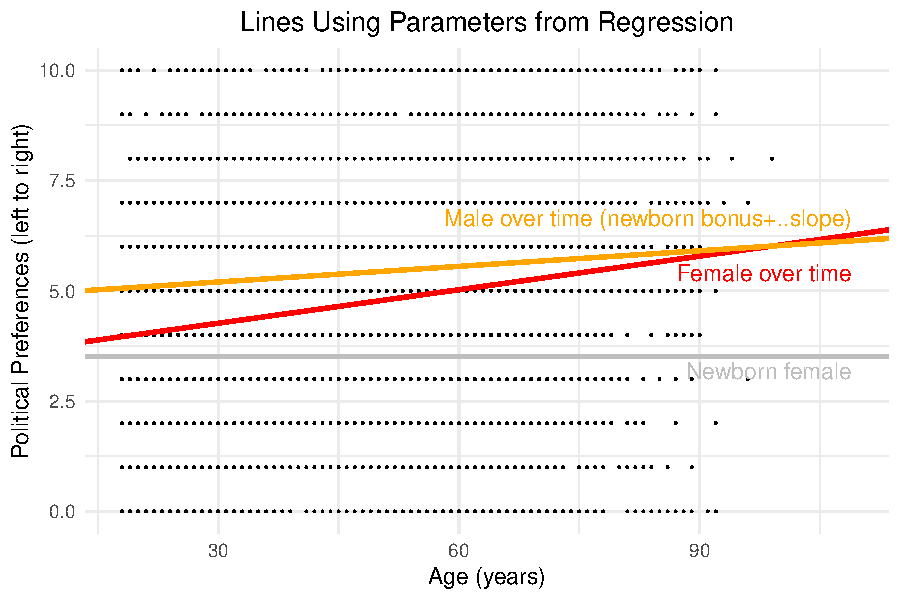
\includegraphics{_main_files/figure-latex/unnamed-chunk-71-1.pdf}

\begin{enumerate}
\def\labelenumi{\arabic{enumi}.}
\setcounter{enumi}{5}
\tightlist
\item
  Following the same logic as in the previous point, you now add the \texttt{LanguageHome} categorical variable with the corresponding interactions. Do the same as in the previous point.
\end{enumerate}

Write the regression here.

\begin{Shaded}
\begin{Highlighting}[]
\CommentTok{\#regression}
\NormalTok{result }\OtherTok{\textless{}{-}} \FunctionTok{lm}\NormalTok{(LeftToRight }\SpecialCharTok{\textasciitilde{}}\NormalTok{ age }\SpecialCharTok{*}\NormalTok{ Sex }\SpecialCharTok{*}\NormalTok{ LanguageHome, }\AttributeTok{data =}\NormalTok{ selects19)}
\FunctionTok{summary}\NormalTok{(result)}
\end{Highlighting}
\end{Shaded}

\begin{verbatim}
## 
## Call:
## lm(formula = LeftToRight ~ age * Sex * LanguageHome, data = selects19)
## 
## Residuals:
##     Min      1Q  Median      3Q     Max 
## -6.1650 -2.0129  0.0157  2.0714  6.1504 
## 
## Coefficients:
##                                               Estimate Std. Error t value
## (Intercept)                                  3.4304317  0.2328505  14.732
## age                                          0.0232899  0.0043627   5.338
## SexMale                                      1.2217711  0.3489102   3.502
## LanguageHomeGerman/Swiss German              0.0096680  0.3214760   0.030
## LanguageHomeItalian                          1.4371272  0.5006063   2.871
## LanguageHomeOther                           -1.1059089  0.6179065  -1.790
## LanguageHomeRomansh                         -2.3047615  3.5040694  -0.658
## age:SexMale                                 -0.0140639  0.0065181  -2.158
## age:LanguageHomeGerman/Swiss German          0.0053104  0.0060152   0.883
## age:LanguageHomeItalian                     -0.0154796  0.0095441  -1.622
## age:LanguageHomeOther                        0.0169430  0.0126468   1.340
## age:LanguageHomeRomansh                      0.0425055  0.0732632   0.580
## SexMale:LanguageHomeGerman/Swiss German      0.1885585  0.4684575   0.403
## SexMale:LanguageHomeItalian                 -0.5629460  0.7043389  -0.799
## SexMale:LanguageHomeOther                    1.6468317  0.9783983   1.683
## SexMale:LanguageHomeRomansh                  1.0259620  4.0396347   0.254
## age:SexMale:LanguageHomeGerman/Swiss German  0.0002337  0.0086831   0.027
## age:SexMale:LanguageHomeItalian              0.0124492  0.0133246   0.934
## age:SexMale:LanguageHomeOther               -0.0265266  0.0193016  -1.374
## age:SexMale:LanguageHomeRomansh              0.0041536  0.0833735   0.050
##                                             Pr(>|t|)    
## (Intercept)                                  < 2e-16 ***
## age                                         9.73e-08 ***
## SexMale                                     0.000466 ***
## LanguageHomeGerman/Swiss German             0.976009    
## LanguageHomeItalian                         0.004109 ** 
## LanguageHomeOther                           0.073543 .  
## LanguageHomeRomansh                         0.510732    
## age:SexMale                                 0.030994 *  
## age:LanguageHomeGerman/Swiss German         0.377368    
## age:LanguageHomeItalian                     0.104877    
## age:LanguageHomeOther                       0.180393    
## age:LanguageHomeRomansh                     0.561819    
## SexMale:LanguageHomeGerman/Swiss German     0.687324    
## SexMale:LanguageHomeItalian                 0.424175    
## SexMale:LanguageHomeOther                   0.092391 .  
## SexMale:LanguageHomeRomansh                 0.799525    
## age:SexMale:LanguageHomeGerman/Swiss German 0.978527    
## age:SexMale:LanguageHomeItalian             0.350189    
## age:SexMale:LanguageHomeOther               0.169395    
## age:SexMale:LanguageHomeRomansh             0.960268    
## ---
## Signif. codes:  0 '***' 0.001 '**' 0.01 '*' 0.05 '.' 0.1 ' ' 1
## 
## Residual standard error: 2.615 on 5887 degrees of freedom
## Multiple R-squared:  0.04377,    Adjusted R-squared:  0.04068 
## F-statistic: 14.18 on 19 and 5887 DF,  p-value: < 2.2e-16
\end{verbatim}

Report and interpret the parameters here.

\begin{Shaded}
\begin{Highlighting}[]
\NormalTok{coeffs }\OtherTok{\textless{}{-}} \FunctionTok{coef}\NormalTok{(result)}
\FunctionTok{cat}\NormalTok{(}\StringTok{\textquotesingle{}Interpreting a regression with ever more interactions is exponentially harder! Thus, find below some few cases aimed at signaling the general logic in the interpretation.\textquotesingle{}}\NormalTok{,}
    
\StringTok{\textquotesingle{}}\SpecialCharTok{\textbackslash{}n\textbackslash{}n}\StringTok{An increase of one year in age across the female Swiss citizens is associated with an average increase in the LeftToRight self{-}declared scale of \textquotesingle{}}\NormalTok{, }\FunctionTok{round}\NormalTok{(}\FunctionTok{unname}\NormalTok{(coeffs[}\DecValTok{2}\NormalTok{]), }\AttributeTok{digits =} \DecValTok{2}\NormalTok{), }\StringTok{\textquotesingle{} }\SpecialCharTok{\textbackslash{}\textquotesingle{}}\StringTok{ideological units}\SpecialCharTok{\textbackslash{}\textquotesingle{}}\StringTok{. Likewise, female newborns whose household speaks mainly in French can be expected to have an average ideological value of \textquotesingle{}}\NormalTok{,}\FunctionTok{round}\NormalTok{(}\FunctionTok{unname}\NormalTok{(coeffs[}\DecValTok{1}\NormalTok{]), }\AttributeTok{digits =} \DecValTok{2}\NormalTok{),}\StringTok{\textquotesingle{}, while a 100 year old female citizens whose household speaks mainly in French can be expected to have an average ideological value of.\textquotesingle{}}\NormalTok{, }\FunctionTok{round}\NormalTok{(}\FunctionTok{unname}\NormalTok{(coeffs[}\DecValTok{1}\NormalTok{]), }\AttributeTok{digits =} \DecValTok{2}\NormalTok{)}\SpecialCharTok{+}\FunctionTok{round}\NormalTok{(}\FunctionTok{unname}\NormalTok{(coeffs[}\DecValTok{2}\NormalTok{]), }\AttributeTok{digits =} \DecValTok{2}\NormalTok{)}\SpecialCharTok{*}\DecValTok{100}\NormalTok{, }

\StringTok{\textquotesingle{}.}\SpecialCharTok{\textbackslash{}n\textbackslash{}n}\StringTok{Similarly, should one observe a random 100 year old male individual whose household speaks mainly in German, we can expected him have an average of \textquotesingle{}}\NormalTok{, }\FunctionTok{round}\NormalTok{(}\FunctionTok{unname}\NormalTok{(coeffs[}\DecValTok{2}\NormalTok{]), }\AttributeTok{digits =} \DecValTok{2}\NormalTok{)}\SpecialCharTok{*}\DecValTok{100}\SpecialCharTok{+}\FunctionTok{round}\NormalTok{(}\FunctionTok{unname}\NormalTok{(coeffs[}\DecValTok{3}\NormalTok{]), }\AttributeTok{digits =} \DecValTok{2}\NormalTok{)}\SpecialCharTok{+}\FunctionTok{round}\NormalTok{(}\FunctionTok{unname}\NormalTok{(coeffs[}\DecValTok{8}\NormalTok{]), }\AttributeTok{digits =} \DecValTok{2}\NormalTok{)}\SpecialCharTok{*}\DecValTok{100}\SpecialCharTok{+}\FunctionTok{round}\NormalTok{(}\FunctionTok{unname}\NormalTok{(coeffs[}\DecValTok{9}\NormalTok{]), }\AttributeTok{digits =} \DecValTok{2}\NormalTok{)}\SpecialCharTok{*}\DecValTok{100}\SpecialCharTok{+}\FunctionTok{round}\NormalTok{(}\FunctionTok{unname}\NormalTok{(coeffs[}\DecValTok{13}\NormalTok{]), }\AttributeTok{digits =} \DecValTok{2}\NormalTok{)}\SpecialCharTok{+}\FunctionTok{round}\NormalTok{(}\FunctionTok{unname}\NormalTok{(coeffs[}\DecValTok{17}\NormalTok{]), }\AttributeTok{digits =} \DecValTok{2}\NormalTok{)}\SpecialCharTok{*}\DecValTok{100}\NormalTok{, }\StringTok{\textquotesingle{} ideological units higher than a female newborn whose household speaks mainly in French. Consequently, the expected ideological value for the former would be of \textquotesingle{}}\NormalTok{, }\FunctionTok{round}\NormalTok{(}\FunctionTok{unname}\NormalTok{(coeffs[}\DecValTok{1}\NormalTok{]), }\AttributeTok{digits =} \DecValTok{2}\NormalTok{)}\SpecialCharTok{+}\FunctionTok{round}\NormalTok{(}\FunctionTok{unname}\NormalTok{(coeffs[}\DecValTok{2}\NormalTok{]), }\AttributeTok{digits =} \DecValTok{2}\NormalTok{)}\SpecialCharTok{*}\DecValTok{100}\SpecialCharTok{+}\FunctionTok{round}\NormalTok{(}\FunctionTok{unname}\NormalTok{(coeffs[}\DecValTok{3}\NormalTok{]), }\AttributeTok{digits =} \DecValTok{2}\NormalTok{)}\SpecialCharTok{+}\FunctionTok{round}\NormalTok{(}\FunctionTok{unname}\NormalTok{(coeffs[}\DecValTok{8}\NormalTok{]), }\AttributeTok{digits =} \DecValTok{2}\NormalTok{)}\SpecialCharTok{*}\DecValTok{100}\SpecialCharTok{+}\FunctionTok{round}\NormalTok{(}\FunctionTok{unname}\NormalTok{(coeffs[}\DecValTok{9}\NormalTok{]), }\AttributeTok{digits =} \DecValTok{2}\NormalTok{)}\SpecialCharTok{*}\DecValTok{100}\SpecialCharTok{+}\FunctionTok{round}\NormalTok{(}\FunctionTok{unname}\NormalTok{(coeffs[}\DecValTok{13}\NormalTok{]), }\AttributeTok{digits =} \DecValTok{2}\NormalTok{)}\SpecialCharTok{+}\FunctionTok{round}\NormalTok{(}\FunctionTok{unname}\NormalTok{(coeffs[}\DecValTok{17}\NormalTok{]), }\AttributeTok{digits =} \DecValTok{2}\NormalTok{)}\SpecialCharTok{*}\DecValTok{100}\NormalTok{)}
\end{Highlighting}
\end{Shaded}

\begin{verbatim}
## Interpreting a regression with ever more interactions is exponentially harder! Thus, find below some few cases aimed at signaling the general logic in the interpretation. 
## 
## An increase of one year in age across the female Swiss citizens is associated with an average increase in the LeftToRight self-declared scale of  0.02  'ideological units'. Likewise, female newborns whose household speaks mainly in French can be expected to have an average ideological value of  3.43 , while a 100 year old female citizens whose household speaks mainly in French can be expected to have an average ideological value of. 5.43 .
## 
## Similarly, should one observe a random 100 year old male individual whose household speaks mainly in German, we can expected him have an average of  3.41  ideological units higher than a female newborn whose household speaks mainly in French. Consequently, the expected ideological value for the former would be of  6.84
\end{verbatim}

Graph some of the main components of the regression output here.

\begin{Shaded}
\begin{Highlighting}[]
\FunctionTok{ggplot}\NormalTok{(selects19, }\FunctionTok{aes}\NormalTok{(}\AttributeTok{x =}\NormalTok{ age, }\AttributeTok{y =}\NormalTok{ LeftToRight)) }\SpecialCharTok{+}  \CommentTok{\# Removed selects19$ from aes(), not necessary}
  \FunctionTok{geom\_point}\NormalTok{(}\AttributeTok{size =} \DecValTok{0}\NormalTok{) }\SpecialCharTok{+}
  \FunctionTok{geom\_abline}\NormalTok{(}\AttributeTok{intercept =} \FunctionTok{unname}\NormalTok{(coeffs[}\DecValTok{1}\NormalTok{]),}
              \AttributeTok{slope =} \DecValTok{0}\NormalTok{, }\AttributeTok{color =} \StringTok{"gray"}\NormalTok{, }\AttributeTok{size =} \DecValTok{1}\NormalTok{) }\SpecialCharTok{+}
  \FunctionTok{geom\_text}\NormalTok{(}\FunctionTok{aes}\NormalTok{(}\AttributeTok{label =} \StringTok{"Newborn female French speaking household"}\NormalTok{,}
                \AttributeTok{x =} \FunctionTok{max}\NormalTok{(selects19}\SpecialCharTok{$}\NormalTok{age)}\SpecialCharTok{+}\DecValTok{10}\NormalTok{,}
                \AttributeTok{y =} \FloatTok{0.1}\SpecialCharTok{+}\FunctionTok{unname}\NormalTok{(coeffs[}\DecValTok{1}\NormalTok{])),}
                \AttributeTok{hjust =} \DecValTok{1}\NormalTok{, }\AttributeTok{vjust =} \DecValTok{0}\NormalTok{, }\AttributeTok{color =} \StringTok{"gray"}\NormalTok{)}\SpecialCharTok{+} 

  \FunctionTok{geom\_abline}\NormalTok{(}\AttributeTok{intercept =} \FunctionTok{unname}\NormalTok{(coeffs[}\DecValTok{1}\NormalTok{]),}
              \AttributeTok{slope =} \FunctionTok{unname}\NormalTok{(coeffs[}\DecValTok{2}\NormalTok{]), }\AttributeTok{color =} \StringTok{"red"}\NormalTok{, }\AttributeTok{size =} \DecValTok{1}\NormalTok{) }\SpecialCharTok{+}
  \FunctionTok{geom\_text}\NormalTok{(}\FunctionTok{aes}\NormalTok{(}\AttributeTok{label =} \StringTok{"Female French speaking household over time"}\NormalTok{,}
                \AttributeTok{x =} \FunctionTok{max}\NormalTok{(selects19}\SpecialCharTok{$}\NormalTok{age)}\SpecialCharTok{+}\DecValTok{10}\NormalTok{,}
                \AttributeTok{y =} \SpecialCharTok{{-}}\FloatTok{1.6}\SpecialCharTok{+}\FunctionTok{unname}\NormalTok{(coeffs[}\DecValTok{1}\NormalTok{]) }\SpecialCharTok{+} \FunctionTok{unname}\NormalTok{(coeffs[}\DecValTok{2}\NormalTok{]) }\SpecialCharTok{*} \FunctionTok{max}\NormalTok{(selects19}\SpecialCharTok{$}\NormalTok{age)),}
                \AttributeTok{hjust =} \DecValTok{1}\NormalTok{, }\AttributeTok{vjust =} \DecValTok{0}\NormalTok{, }\AttributeTok{color =} \StringTok{"red"}\NormalTok{) }\SpecialCharTok{+}

  \FunctionTok{geom\_abline}\NormalTok{(}\AttributeTok{intercept =} \FunctionTok{unname}\NormalTok{(coeffs[}\DecValTok{1}\NormalTok{])}\SpecialCharTok{+}\FunctionTok{unname}\NormalTok{(coeffs[}\DecValTok{3}\NormalTok{]),}
              \AttributeTok{slope =} \FunctionTok{unname}\NormalTok{(coeffs[}\DecValTok{2}\NormalTok{])}\SpecialCharTok{+}\FunctionTok{unname}\NormalTok{(coeffs[}\DecValTok{8}\NormalTok{]), }\AttributeTok{color =} \StringTok{"orange"}\NormalTok{, }\AttributeTok{size =} \DecValTok{1}\NormalTok{) }\SpecialCharTok{+}
  \FunctionTok{geom\_text}\NormalTok{(}\FunctionTok{aes}\NormalTok{(}\AttributeTok{label =} \StringTok{"Male French household over time (newborn bonus+Δslope)"}\NormalTok{,}
                \AttributeTok{x =} \FunctionTok{max}\NormalTok{(selects19}\SpecialCharTok{$}\NormalTok{age)}\SpecialCharTok{+}\DecValTok{10}\NormalTok{,}
                \AttributeTok{y =} \FloatTok{0.4}\SpecialCharTok{+}\FunctionTok{unname}\NormalTok{(coeffs[}\DecValTok{1}\NormalTok{])}\SpecialCharTok{+}\FunctionTok{unname}\NormalTok{(coeffs[}\DecValTok{3}\NormalTok{]) }\SpecialCharTok{+}\NormalTok{ (}\FunctionTok{unname}\NormalTok{(coeffs[}\DecValTok{2}\NormalTok{])}\SpecialCharTok{+}\FunctionTok{unname}\NormalTok{(coeffs[}\DecValTok{8}\NormalTok{])) }\SpecialCharTok{*} \FunctionTok{max}\NormalTok{(selects19}\SpecialCharTok{$}\NormalTok{age)}\SpecialCharTok{+}\FloatTok{0.2}\NormalTok{),}
                \AttributeTok{hjust =} \DecValTok{1}\NormalTok{, }\AttributeTok{vjust =} \DecValTok{0}\NormalTok{, }\AttributeTok{color =} \StringTok{"orange"}\NormalTok{) }\SpecialCharTok{+}
  
  \FunctionTok{geom\_abline}\NormalTok{(}\AttributeTok{intercept =} \FunctionTok{unname}\NormalTok{(coeffs[}\DecValTok{1}\NormalTok{])}\SpecialCharTok{+}\FunctionTok{unname}\NormalTok{(coeffs[}\DecValTok{3}\NormalTok{])}\SpecialCharTok{+}\FunctionTok{unname}\NormalTok{(coeffs[}\DecValTok{13}\NormalTok{]),}
              \AttributeTok{slope =} \FunctionTok{unname}\NormalTok{(coeffs[}\DecValTok{2}\NormalTok{])}\SpecialCharTok{+}\FunctionTok{unname}\NormalTok{(coeffs[}\DecValTok{8}\NormalTok{])}\SpecialCharTok{+}\FunctionTok{unname}\NormalTok{(coeffs[}\DecValTok{17}\NormalTok{]), }\AttributeTok{color =} \StringTok{"purple"}\NormalTok{, }\AttributeTok{size =} \DecValTok{1}\NormalTok{) }\SpecialCharTok{+}
  \FunctionTok{geom\_text}\NormalTok{(}\FunctionTok{aes}\NormalTok{(}\AttributeTok{label =} \StringTok{"Male German household over time (newborn \& ling. bonus+Δslope)"}\NormalTok{,}
                \AttributeTok{x =} \FunctionTok{max}\NormalTok{(selects19}\SpecialCharTok{$}\NormalTok{age)}\SpecialCharTok{+}\DecValTok{10}\NormalTok{,}
                \AttributeTok{y =} \FloatTok{1.2}\SpecialCharTok{+}\FunctionTok{unname}\NormalTok{(coeffs[}\DecValTok{1}\NormalTok{])}\SpecialCharTok{+}\FunctionTok{unname}\NormalTok{(coeffs[}\DecValTok{3}\NormalTok{])}\SpecialCharTok{+}\FunctionTok{unname}\NormalTok{(coeffs[}\DecValTok{13}\NormalTok{]) }\SpecialCharTok{+}\NormalTok{ (}\FunctionTok{unname}\NormalTok{(coeffs[}\DecValTok{2}\NormalTok{])}\SpecialCharTok{+}\FunctionTok{unname}\NormalTok{(coeffs[}\DecValTok{8}\NormalTok{])}\SpecialCharTok{+}\FunctionTok{unname}\NormalTok{(coeffs[}\DecValTok{17}\NormalTok{])) }\SpecialCharTok{*} \FunctionTok{max}\NormalTok{(selects19}\SpecialCharTok{$}\NormalTok{age)}\SpecialCharTok{+}\FloatTok{0.2}\NormalTok{),}
                \AttributeTok{hjust =} \DecValTok{1}\NormalTok{, }\AttributeTok{vjust =} \DecValTok{0}\NormalTok{, }\AttributeTok{color =} \StringTok{"purple"}\NormalTok{) }\SpecialCharTok{+}  
  \CommentTok{\# geom\_abline(intercept = unname(coeffs[1])+unname(coeffs[3]),}
  \CommentTok{\#             slope = unname(coeffs[2])+unname(coeffs[4]), color = "blue", size = 1) +}
  \CommentTok{\# geom\_text(aes(label = "Int.(fem)+Male+Age*Male",}
  \CommentTok{\#               x = max(selects19$age)+10,}
  \CommentTok{\#               y = 0.3+unname(coeffs[1])+unname(coeffs[3]) + (unname(coeffs[2])+unname(coeffs[4])) * max(selects19$age)+0.2),}
  \CommentTok{\#               hjust = 1, vjust = 0, color = "blue") +}
  
  \FunctionTok{theme\_minimal}\NormalTok{() }\SpecialCharTok{+}
  \FunctionTok{theme}\NormalTok{(}\AttributeTok{plot.title =} \FunctionTok{element\_text}\NormalTok{(}\AttributeTok{hjust =} \FloatTok{0.5}\NormalTok{)) }\SpecialCharTok{+}
  \FunctionTok{labs}\NormalTok{(}
    \AttributeTok{x =} \StringTok{"Age (years)"}\NormalTok{,}
    \AttributeTok{y =} \StringTok{"Political Preferences (left to right)"}\NormalTok{,}
    \AttributeTok{title =} \StringTok{"Lines Using Parameters from Regression"}
\NormalTok{  )}
\end{Highlighting}
\end{Shaded}

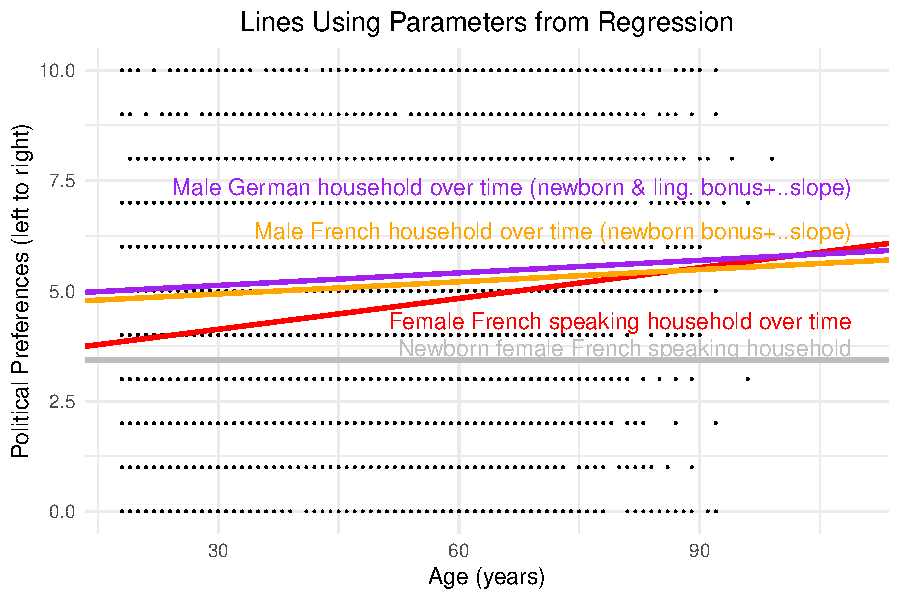
\includegraphics{_main_files/figure-latex/unnamed-chunk-74-1.pdf}

\emph{{Ojo: Check that interpretations have the right parameters!}.}

\hypertarget{interactive-line-plot}{%
\section{Interactive Line Plot}\label{interactive-line-plot}}

\emph{{Should we exploit this here or somewhere else? I can make it work in R, but not in the book yet. If needed, I can check it out.}.}

\begin{Shaded}
\begin{Highlighting}[]
\CommentTok{\# \# Example data frame}
\CommentTok{\# data \textless{}{-} data.frame(}
\CommentTok{\#   x = rnorm(100),}
\CommentTok{\#   y = rnorm(100)}
\CommentTok{\# )}
\CommentTok{\# }
\CommentTok{\# \# Shiny server function}
\CommentTok{\# server \textless{}{-} function(input, output) \{}
\CommentTok{\#   output$scatterPlot \textless{}{-} renderPlot(\{}
\CommentTok{\#     ggplot(data, aes(x = x, y = y)) +  }
\CommentTok{\#       geom\_point(size = 0) +}
\CommentTok{\#       geom\_abline(intercept = input$intercept, slope = input$slope, color = "red", size = 1)}
\CommentTok{\#   \})}
\CommentTok{\# \}}
\CommentTok{\# }
\CommentTok{\# \# Example data frame}
\CommentTok{\# data \textless{}{-} data.frame(}
\CommentTok{\#   x = rnorm(100),}
\CommentTok{\#   y = rnorm(100)}
\CommentTok{\# )}
\CommentTok{\# }
\CommentTok{\# \# Shiny server function}
\CommentTok{\# server \textless{}{-} function(input, output) \{}
\CommentTok{\#   output$scatterPlot \textless{}{-} renderPlot(\{}
\CommentTok{\#     ggplot(data, aes(x = x, y = y)) +  }
\CommentTok{\#       geom\_point(size = 0) +}
\CommentTok{\#       geom\_abline(intercept = input$intercept, slope = input$slope, color = "red", size = 1)}
\CommentTok{\#   \})}
\CommentTok{\# \}}
\CommentTok{\# }
\CommentTok{\# update.packages(ask = FALSE)}
\CommentTok{\# }
\CommentTok{\# }
\CommentTok{\# library(shiny)}
\CommentTok{\# library(ggplot2)}
\CommentTok{\# }
\CommentTok{\# ui \textless{}{-} fluidPage(}
\CommentTok{\#   titlePanel("Interactive Line Plot"),}
\CommentTok{\#   sidebarLayout(}
\CommentTok{\#     sidebarPanel(}
\CommentTok{\#       sliderInput("intercept", "Intercept:", min = {-}10, max = 10, value = 0),}
\CommentTok{\#       sliderInput("slope", "Slope:", min = {-}10, max = 10, value = 1)}
\CommentTok{\#     ),}
\CommentTok{\#     mainPanel(}
\CommentTok{\#       plotOutput("scatterPlot")}
\CommentTok{\#     )}
\CommentTok{\#   )}
\CommentTok{\# )}
\CommentTok{\# }
\CommentTok{\# server \textless{}{-} function(input, output) \{}
\CommentTok{\#   output$scatterPlot \textless{}{-} renderPlot(\{}
\CommentTok{\#     ggplot(data, aes(x = x, y = y)) +}
\CommentTok{\#       geom\_point(size = 0) +}
\CommentTok{\#       geom\_abline(intercept = input$intercept, slope = input$slope, color = "red", size = 1)}
\CommentTok{\#   \})}
\CommentTok{\# \}}
\CommentTok{\# }
\CommentTok{\# shinyApp(ui = ui, server = server)}
\end{Highlighting}
\end{Shaded}

\hypertarget{simulated-data-1}{%
\subsection{Simulated data}\label{simulated-data-1}}

\begin{enumerate}
\def\labelenumi{\arabic{enumi}.}
\tightlist
\item
  In order to see the logic behind the \(R^2\), first estimate the linear regression of \texttt{LeftToRight} on \texttt{Age}. Generate the variable \texttt{predicted\_LeftToRight} with the generated parameters using \href{https://www.statology.org/r-lm-predict/}{\texttt{predict()}} from the point 3 of the previous section (i.e., the one using real data).Generate the graph \texttt{predicted\_LeftToRight} vs \texttt{Age}.
\end{enumerate}

Report the regression here.

\begin{Shaded}
\begin{Highlighting}[]
\NormalTok{result }\OtherTok{\textless{}{-}} \FunctionTok{lm}\NormalTok{(LeftToRight }\SpecialCharTok{\textasciitilde{}}\NormalTok{ age, }\AttributeTok{data =}\NormalTok{ selects19)}
\NormalTok{selects19}\SpecialCharTok{$}\NormalTok{predicted\_LeftToRight }\OtherTok{\textless{}{-}} \FunctionTok{predict}\NormalTok{(result)}

\NormalTok{coeffs1 }\OtherTok{\textless{}{-}} \FunctionTok{coef}\NormalTok{(result)}
\NormalTok{rsq\_sd1 }\OtherTok{\textless{}{-}} \FunctionTok{summary}\NormalTok{(result)}\SpecialCharTok{$}\NormalTok{r.squared}
\FunctionTok{cat}\NormalTok{(}\StringTok{\textquotesingle{}The R2 is: \textquotesingle{}}\NormalTok{, rsq\_sd1, }\StringTok{\textquotesingle{}}\SpecialCharTok{\textbackslash{}n\textbackslash{}n}\StringTok{Intercept:\textquotesingle{}}\NormalTok{,}\FunctionTok{unname}\NormalTok{(coeffs1[}\DecValTok{1}\NormalTok{]), }\StringTok{\textquotesingle{}}\SpecialCharTok{\textbackslash{}n\textbackslash{}n}\StringTok{Slope:\textquotesingle{}}\NormalTok{, }\FunctionTok{unname}\NormalTok{(coeffs1[}\DecValTok{2}\NormalTok{]))}
\end{Highlighting}
\end{Shaded}

\begin{verbatim}
## The R2 is:  0.0161515 
## 
## Intercept: 4.122055 
## 
## Slope: 0.01948902
\end{verbatim}

Report the graph here.

\begin{Shaded}
\begin{Highlighting}[]
\CommentTok{\# Calculate means for Y and X}
\NormalTok{mean\_LeftRight }\OtherTok{\textless{}{-}} \FunctionTok{mean}\NormalTok{(selects19}\SpecialCharTok{$}\NormalTok{LeftToRight, }\AttributeTok{na.rm =} \ConstantTok{TRUE}\NormalTok{)}
\NormalTok{mean\_age }\OtherTok{\textless{}{-}} \FunctionTok{mean}\NormalTok{(selects19}\SpecialCharTok{$}\NormalTok{age, }\AttributeTok{na.rm =} \ConstantTok{TRUE}\NormalTok{)}

\CommentTok{\# Create a scatter plot}
\FunctionTok{ggplot}\NormalTok{(selects19, }\FunctionTok{aes}\NormalTok{(}\AttributeTok{x =}\NormalTok{ age, }\AttributeTok{y =}\NormalTok{ predicted\_LeftToRight)) }\SpecialCharTok{+}
  \FunctionTok{geom\_smooth}\NormalTok{(}\AttributeTok{method =} \StringTok{"lm"}\NormalTok{, }\AttributeTok{formula =}\NormalTok{ y }\SpecialCharTok{\textasciitilde{}}\NormalTok{ x, }\AttributeTok{se =} \ConstantTok{FALSE}\NormalTok{, }\AttributeTok{color =} \StringTok{"red"}\NormalTok{) }\SpecialCharTok{+}  \CommentTok{\# Adding the regression line}
  \FunctionTok{geom\_hline}\NormalTok{(}\AttributeTok{yintercept =}\NormalTok{ mean\_LeftRight, }\AttributeTok{linetype =} \StringTok{"dashed"}\NormalTok{, }\AttributeTok{color =} \StringTok{"green"}\NormalTok{) }\SpecialCharTok{+}  \CommentTok{\# Horizontal line at the mean of y}
  \FunctionTok{geom\_vline}\NormalTok{(}\AttributeTok{xintercept =}\NormalTok{ mean\_age, }\AttributeTok{linetype =} \StringTok{"dashed"}\NormalTok{, }\AttributeTok{color =} \StringTok{"orange"}\NormalTok{) }\SpecialCharTok{+}  \CommentTok{\# Vertical line at the mean of x}
  \FunctionTok{scale\_y\_continuous}\NormalTok{(}
    \AttributeTok{limits =} \FunctionTok{c}\NormalTok{(}\DecValTok{0}\NormalTok{, }\DecValTok{10}\NormalTok{),}
    \AttributeTok{breaks =} \FunctionTok{seq}\NormalTok{(}\DecValTok{0}\NormalTok{, }\DecValTok{10}\NormalTok{, }\AttributeTok{by =} \DecValTok{1}\NormalTok{)  }
\NormalTok{  ) }\SpecialCharTok{+}
  \FunctionTok{theme\_minimal}\NormalTok{() }\SpecialCharTok{+}
  \FunctionTok{theme}\NormalTok{(}
    \AttributeTok{plot.title =} \FunctionTok{element\_text}\NormalTok{(}\AttributeTok{hjust =} \FloatTok{0.5}\NormalTok{), }\CommentTok{\# Center the plot title}
    \AttributeTok{panel.grid.major.y =} \FunctionTok{element\_line}\NormalTok{(}\AttributeTok{color =} \StringTok{"grey80"}\NormalTok{, }\AttributeTok{size =} \FloatTok{0.5}\NormalTok{), }\CommentTok{\# Style for major Y grid lines}
    \AttributeTok{panel.grid.minor.y =} \FunctionTok{element\_blank}\NormalTok{() }\CommentTok{\# Remove minor Y grid lines}
\NormalTok{  ) }\SpecialCharTok{+}
  \FunctionTok{labs}\NormalTok{(}
    \AttributeTok{x =} \StringTok{"Age (years)"}\NormalTok{,}
    \AttributeTok{y =} \StringTok{"Political Preferences (left to right)"}\NormalTok{,}
    \AttributeTok{title =} \StringTok{"Scatter plot Age vs. Political Preferences (determ. sim.)"}
\NormalTok{  )}
\end{Highlighting}
\end{Shaded}

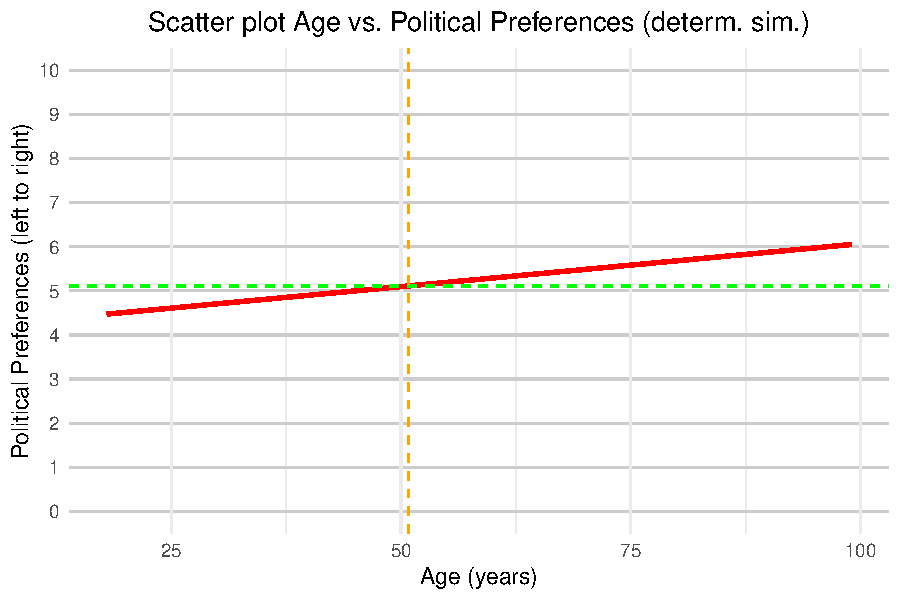
\includegraphics{_main_files/figure-latex/unnamed-chunk-77-1.pdf}

\begin{enumerate}
\def\labelenumi{\arabic{enumi}.}
\setcounter{enumi}{1}
\tightlist
\item
  Now generate the normally distributed residuals with mean zero and the same variance as the residuals of the model from the previous point.
\end{enumerate}

\begin{Shaded}
\begin{Highlighting}[]
\CommentTok{\# Calculate the variance of the residuals}
\NormalTok{selects19}\SpecialCharTok{$}\NormalTok{residual }\OtherTok{\textless{}{-}} \FunctionTok{resid}\NormalTok{(result)}
\NormalTok{residual\_sd }\OtherTok{\textless{}{-}} \FunctionTok{sqrt}\NormalTok{(}\FunctionTok{var}\NormalTok{(}\FunctionTok{resid}\NormalTok{(result)))}

\CommentTok{\# Set the seed for reproducibility}
\FunctionTok{set.seed}\NormalTok{(}\DecValTok{0}\NormalTok{)}
\NormalTok{selects19}\SpecialCharTok{$}\NormalTok{NormResiduals1 }\OtherTok{\textless{}{-}} \FunctionTok{rnorm}\NormalTok{(}\FunctionTok{nrow}\NormalTok{(selects19), }\AttributeTok{mean =} \DecValTok{0}\NormalTok{, }\AttributeTok{sd =}\NormalTok{ residual\_sd)}
\end{Highlighting}
\end{Shaded}

\begin{enumerate}
\def\labelenumi{\arabic{enumi}.}
\setcounter{enumi}{2}
\tightlist
\item
  Simulate new data using both the deterministic (i.e., the the parameters estimated immediately above) and stochastic component (i.e., the residuals form the previous point). Graph the simulated data.
\end{enumerate}

\begin{Shaded}
\begin{Highlighting}[]
\NormalTok{selects19}\SpecialCharTok{$}\NormalTok{Sim\_LeftToRight\_Det\_Stoch }\OtherTok{\textless{}{-}}\NormalTok{ selects19}\SpecialCharTok{$}\NormalTok{predicted\_LeftToRight }\SpecialCharTok{+}\NormalTok{ selects19}\SpecialCharTok{$}\NormalTok{NormResiduals1}

\CommentTok{\#Means for Y and X}
\NormalTok{mean\_LeftRight }\OtherTok{\textless{}{-}} \FunctionTok{mean}\NormalTok{(selects19}\SpecialCharTok{$}\NormalTok{Sim\_LeftToRight\_Det\_Stoch, }\AttributeTok{na.rm =} \ConstantTok{TRUE}\NormalTok{)}
\NormalTok{mean\_age }\OtherTok{\textless{}{-}} \FunctionTok{mean}\NormalTok{(selects19}\SpecialCharTok{$}\NormalTok{age, }\AttributeTok{na.rm =} \ConstantTok{TRUE}\NormalTok{)}

\CommentTok{\# Create a scatter plot}
\FunctionTok{ggplot}\NormalTok{(selects19, }\FunctionTok{aes}\NormalTok{(}\AttributeTok{x =}\NormalTok{ age, }\AttributeTok{y =}\NormalTok{ Sim\_LeftToRight\_Det\_Stoch)) }\SpecialCharTok{+}
  \FunctionTok{geom\_point}\NormalTok{(}\AttributeTok{size =} \DecValTok{0}\NormalTok{) }\SpecialCharTok{+}
  \FunctionTok{geom\_smooth}\NormalTok{(}\AttributeTok{method =} \StringTok{"lm"}\NormalTok{, }\AttributeTok{formula =}\NormalTok{ y }\SpecialCharTok{\textasciitilde{}}\NormalTok{ x, }\AttributeTok{se =} \ConstantTok{FALSE}\NormalTok{, }\AttributeTok{color =} \StringTok{"red"}\NormalTok{) }\SpecialCharTok{+}  \CommentTok{\# Adding the regression line}
  \FunctionTok{geom\_hline}\NormalTok{(}\AttributeTok{yintercept =}\NormalTok{ mean\_LeftRight, }\AttributeTok{linetype =} \StringTok{"dashed"}\NormalTok{, }\AttributeTok{color =} \StringTok{"green"}\NormalTok{) }\SpecialCharTok{+}  \CommentTok{\# Horizontal line at the mean of y}
  \FunctionTok{geom\_vline}\NormalTok{(}\AttributeTok{xintercept =}\NormalTok{ mean\_age, }\AttributeTok{linetype =} \StringTok{"dashed"}\NormalTok{, }\AttributeTok{color =} \StringTok{"orange"}\NormalTok{) }\SpecialCharTok{+}  \CommentTok{\# Vertical line at the mean of x}
  \FunctionTok{theme\_minimal}\NormalTok{() }\SpecialCharTok{+}
  \FunctionTok{theme}\NormalTok{(}\AttributeTok{plot.title =} \FunctionTok{element\_text}\NormalTok{(}\AttributeTok{hjust =} \FloatTok{0.5}\NormalTok{)) }\SpecialCharTok{+}
  \FunctionTok{scale\_y\_continuous}\NormalTok{(}
    \AttributeTok{limits =} \FunctionTok{c}\NormalTok{(}\DecValTok{0}\NormalTok{, }\DecValTok{10}\NormalTok{),}
    \AttributeTok{breaks =} \FunctionTok{seq}\NormalTok{(}\DecValTok{0}\NormalTok{, }\DecValTok{10}\NormalTok{, }\AttributeTok{by =} \DecValTok{1}\NormalTok{)) }\SpecialCharTok{+}
  \FunctionTok{theme\_minimal}\NormalTok{() }\SpecialCharTok{+}
  \FunctionTok{theme}\NormalTok{(}
    \AttributeTok{plot.title =} \FunctionTok{element\_text}\NormalTok{(}\AttributeTok{hjust =} \FloatTok{0.5}\NormalTok{), }\CommentTok{\# Center the plot title}
    \AttributeTok{panel.grid.major.y =} \FunctionTok{element\_line}\NormalTok{(}\AttributeTok{color =} \StringTok{"grey80"}\NormalTok{, }\AttributeTok{size =} \FloatTok{0.5}\NormalTok{), }\CommentTok{\# Style for major Y grid lines}
    \AttributeTok{panel.grid.minor.y =} \FunctionTok{element\_blank}\NormalTok{() }\CommentTok{\# Remove minor Y grid lines}
\NormalTok{  ) }\SpecialCharTok{+}
  \FunctionTok{labs}\NormalTok{(}
    \AttributeTok{x =} \StringTok{"Age (years)"}\NormalTok{,}
    \AttributeTok{y =} \StringTok{"Simulation: Political Preferences (left to right)"}\NormalTok{,}
    \AttributeTok{title =} \StringTok{"Scatter plot Age vs. Political Preferences }\SpecialCharTok{\textbackslash{}n}\StringTok{(determ.\& stoch. sim.)"}
\NormalTok{  )}
\end{Highlighting}
\end{Shaded}

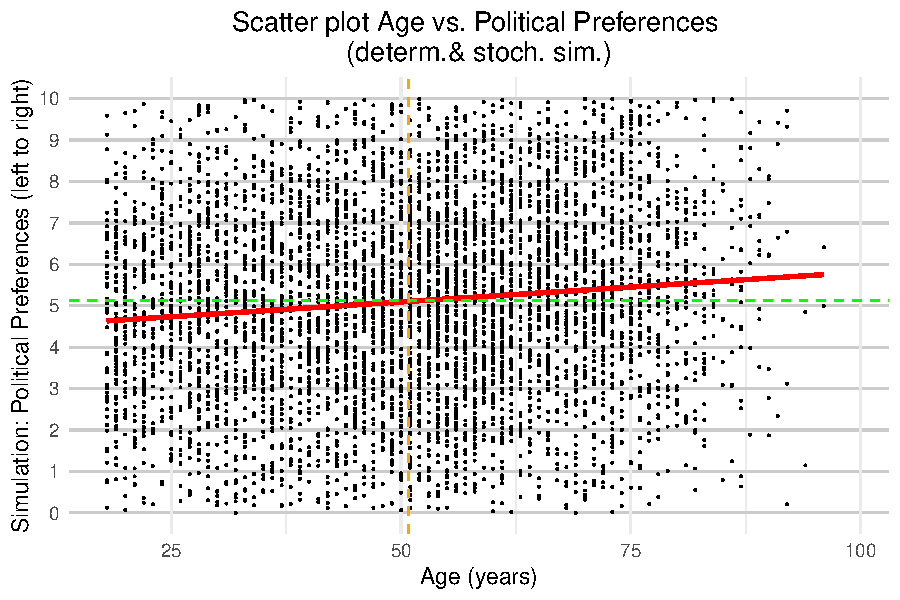
\includegraphics{_main_files/figure-latex/unnamed-chunk-79-1.pdf}

\begin{enumerate}
\def\labelenumi{\arabic{enumi}.}
\setcounter{enumi}{3}
\tightlist
\item
  Now, estimate the regression between the real \texttt{age} and simulated \texttt{Sim\_LeftToRight\_Det\_Stoch}. Once you do that, generate the \(R^2\) for the model.
\end{enumerate}

\begin{Shaded}
\begin{Highlighting}[]
\NormalTok{result }\OtherTok{\textless{}{-}} \FunctionTok{lm}\NormalTok{(LeftToRight }\SpecialCharTok{\textasciitilde{}}\NormalTok{ age, }\AttributeTok{data =}\NormalTok{ selects19)}
\NormalTok{rsq\_sd1 }\OtherTok{\textless{}{-}} \FunctionTok{summary}\NormalTok{(result)}\SpecialCharTok{$}\NormalTok{r.squared}
\FunctionTok{cat}\NormalTok{(}\StringTok{\textquotesingle{}The R2 is: \textquotesingle{}}\NormalTok{, rsq\_sd1)}
\end{Highlighting}
\end{Shaded}

\begin{verbatim}
## The R2 is:  0.0161515
\end{verbatim}

\begin{enumerate}
\def\labelenumi{\arabic{enumi}.}
\setcounter{enumi}{4}
\tightlist
\item
  Repeat the previous three points but use half the standard deviation of the model of point 1. Is the \(R^2\) lower now? Why? See \href{https://en.wikipedia.org/wiki/Coefficient_of_determination}{this} entry to understand the intuition: pay special attention to the graph with the red and blue squares.
\end{enumerate}

Generate the residuals here.

\begin{Shaded}
\begin{Highlighting}[]
\CommentTok{\# Set the seed for reproducibility}
\FunctionTok{set.seed}\NormalTok{(}\DecValTok{0}\NormalTok{)}
\NormalTok{selects19}\SpecialCharTok{$}\NormalTok{NormResiduals10 }\OtherTok{\textless{}{-}} \FunctionTok{rnorm}\NormalTok{(}\FunctionTok{nrow}\NormalTok{(selects19), }\AttributeTok{mean =} \DecValTok{0}\NormalTok{, }\AttributeTok{sd =}\NormalTok{ residual\_sd}\SpecialCharTok{*}\FloatTok{0.1}\NormalTok{)}
\end{Highlighting}
\end{Shaded}

Simulate new data and graph it here.

\begin{Shaded}
\begin{Highlighting}[]
\NormalTok{selects19}\SpecialCharTok{$}\NormalTok{Sim\_LeftToRight\_Det\_Stoch\_sd10 }\OtherTok{\textless{}{-}}\NormalTok{ selects19}\SpecialCharTok{$}\NormalTok{predicted\_LeftToRight }\SpecialCharTok{+}\NormalTok{ selects19}\SpecialCharTok{$}\NormalTok{NormResiduals10}

\CommentTok{\#Means for Y and X}
\NormalTok{mean\_LeftRight }\OtherTok{\textless{}{-}} \FunctionTok{mean}\NormalTok{(selects19}\SpecialCharTok{$}\NormalTok{Sim\_LeftToRight\_Det\_Stoch\_sd10, }\AttributeTok{na.rm =} \ConstantTok{TRUE}\NormalTok{)}
\NormalTok{mean\_age }\OtherTok{\textless{}{-}} \FunctionTok{mean}\NormalTok{(selects19}\SpecialCharTok{$}\NormalTok{age, }\AttributeTok{na.rm =} \ConstantTok{TRUE}\NormalTok{)}

\CommentTok{\# Create a scatter plot}
\FunctionTok{ggplot}\NormalTok{(selects19, }\FunctionTok{aes}\NormalTok{(}\AttributeTok{x =}\NormalTok{ age, }\AttributeTok{y =}\NormalTok{ Sim\_LeftToRight\_Det\_Stoch\_sd10)) }\SpecialCharTok{+}
  \FunctionTok{geom\_point}\NormalTok{(}\AttributeTok{size =} \DecValTok{0}\NormalTok{) }\SpecialCharTok{+}
  \FunctionTok{geom\_smooth}\NormalTok{(}\AttributeTok{method =} \StringTok{"lm"}\NormalTok{, }\AttributeTok{formula =}\NormalTok{ y }\SpecialCharTok{\textasciitilde{}}\NormalTok{ x, }\AttributeTok{se =} \ConstantTok{FALSE}\NormalTok{, }\AttributeTok{color =} \StringTok{"red"}\NormalTok{) }\SpecialCharTok{+}  \CommentTok{\# Adding the regression line}
  \FunctionTok{geom\_hline}\NormalTok{(}\AttributeTok{yintercept =}\NormalTok{ mean\_LeftRight, }\AttributeTok{linetype =} \StringTok{"dashed"}\NormalTok{, }\AttributeTok{color =} \StringTok{"green"}\NormalTok{) }\SpecialCharTok{+}  \CommentTok{\# Horizontal line at the mean of y}
  \FunctionTok{geom\_vline}\NormalTok{(}\AttributeTok{xintercept =}\NormalTok{ mean\_age, }\AttributeTok{linetype =} \StringTok{"dashed"}\NormalTok{, }\AttributeTok{color =} \StringTok{"orange"}\NormalTok{) }\SpecialCharTok{+}  \CommentTok{\# Vertical line at the mean of x}
  \FunctionTok{scale\_y\_continuous}\NormalTok{(}
    \AttributeTok{limits =} \FunctionTok{c}\NormalTok{(}\DecValTok{0}\NormalTok{, }\DecValTok{10}\NormalTok{),}
    \AttributeTok{breaks =} \FunctionTok{seq}\NormalTok{(}\DecValTok{0}\NormalTok{, }\DecValTok{10}\NormalTok{, }\AttributeTok{by =} \DecValTok{1}\NormalTok{)) }\SpecialCharTok{+}
  \FunctionTok{theme\_minimal}\NormalTok{() }\SpecialCharTok{+}
  \FunctionTok{theme}\NormalTok{(}\AttributeTok{plot.title =} \FunctionTok{element\_text}\NormalTok{(}\AttributeTok{hjust =} \FloatTok{0.5}\NormalTok{)) }\SpecialCharTok{+}
  \FunctionTok{labs}\NormalTok{(}
    \AttributeTok{x =} \StringTok{"Age (years)"}\NormalTok{,}
    \AttributeTok{y =} \StringTok{"Simulated data (half sd): Political Preferences (left to right)"}\NormalTok{,}
    \AttributeTok{title =} \StringTok{"Scatter plot Age vs. Political Preferences"}
\NormalTok{  )}
\end{Highlighting}
\end{Shaded}

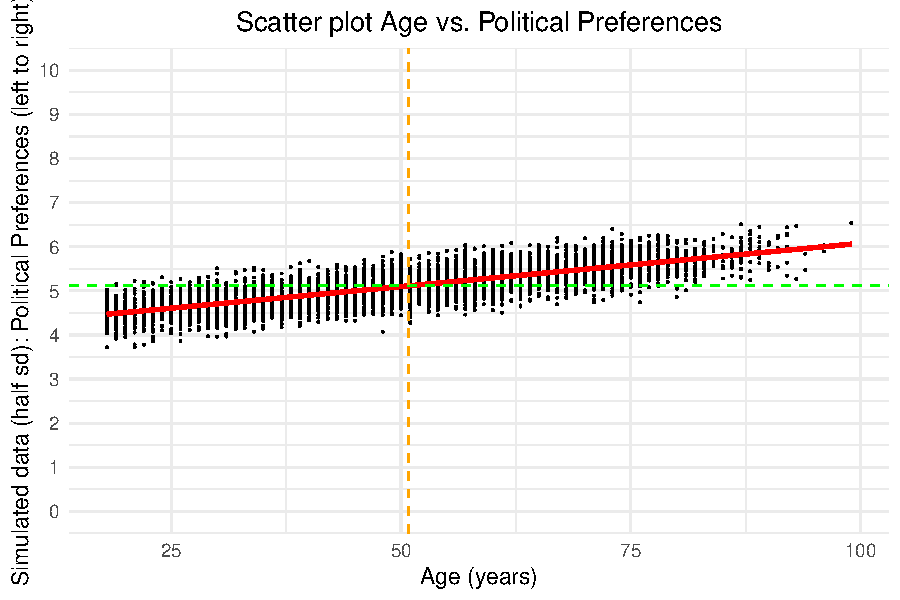
\includegraphics{_main_files/figure-latex/unnamed-chunk-82-1.pdf}

Report the new \(R^2\) here:

\begin{Shaded}
\begin{Highlighting}[]
\NormalTok{result }\OtherTok{\textless{}{-}} \FunctionTok{lm}\NormalTok{(Sim\_LeftToRight\_Det\_Stoch\_sd10 }\SpecialCharTok{\textasciitilde{}}\NormalTok{ age, }\AttributeTok{data =}\NormalTok{ selects19)}
\NormalTok{rsq\_sd10 }\OtherTok{\textless{}{-}} \FunctionTok{summary}\NormalTok{(result)}\SpecialCharTok{$}\NormalTok{r.squared}
\FunctionTok{cat}\NormalTok{(}\StringTok{\textquotesingle{}The R2 is: \textquotesingle{}}\NormalTok{, rsq\_sd10)}
\end{Highlighting}
\end{Shaded}

\begin{verbatim}
## The R2 is:  0.625503
\end{verbatim}

\begin{enumerate}
\def\labelenumi{\arabic{enumi}.}
\setcounter{enumi}{5}
\tightlist
\item
  Repeat the previous point but use a hundredth the standard deviation of the model of point 1. Is the \(R^2\) lower now? Why?
\end{enumerate}

Generate the residuals here.

\begin{Shaded}
\begin{Highlighting}[]
\CommentTok{\# Set the seed for reproducibility}
\FunctionTok{set.seed}\NormalTok{(}\DecValTok{0}\NormalTok{)}
\NormalTok{selects19}\SpecialCharTok{$}\NormalTok{NormResiduals100 }\OtherTok{\textless{}{-}} \FunctionTok{rnorm}\NormalTok{(}\FunctionTok{nrow}\NormalTok{(selects19), }\AttributeTok{mean =} \DecValTok{0}\NormalTok{, }\AttributeTok{sd =}\NormalTok{ residual\_sd}\SpecialCharTok{*}\FloatTok{0.01}\NormalTok{)}
\end{Highlighting}
\end{Shaded}

Simulate new data and graph it here.

\begin{Shaded}
\begin{Highlighting}[]
\NormalTok{selects19}\SpecialCharTok{$}\NormalTok{Sim\_LeftToRight\_Det\_Stoch\_hsd }\OtherTok{\textless{}{-}}\NormalTok{ selects19}\SpecialCharTok{$}\NormalTok{predicted\_LeftToRight }\SpecialCharTok{+}\NormalTok{ selects19}\SpecialCharTok{$}\NormalTok{NormResiduals100}

\CommentTok{\#Means for Y and X}
\NormalTok{mean\_LeftRight }\OtherTok{\textless{}{-}} \FunctionTok{mean}\NormalTok{(selects19}\SpecialCharTok{$}\NormalTok{Sim\_LeftToRight\_Det\_Stoch\_hsd, }\AttributeTok{na.rm =} \ConstantTok{TRUE}\NormalTok{)}
\NormalTok{mean\_age }\OtherTok{\textless{}{-}} \FunctionTok{mean}\NormalTok{(selects19}\SpecialCharTok{$}\NormalTok{age, }\AttributeTok{na.rm =} \ConstantTok{TRUE}\NormalTok{)}

\CommentTok{\# Create a scatter plot}
\FunctionTok{ggplot}\NormalTok{(selects19, }\FunctionTok{aes}\NormalTok{(}\AttributeTok{x =}\NormalTok{ age, }\AttributeTok{y =}\NormalTok{ Sim\_LeftToRight\_Det\_Stoch\_hsd)) }\SpecialCharTok{+}
  \FunctionTok{geom\_point}\NormalTok{(}\AttributeTok{size =} \DecValTok{0}\NormalTok{) }\SpecialCharTok{+}
  \FunctionTok{geom\_smooth}\NormalTok{(}\AttributeTok{method =} \StringTok{"lm"}\NormalTok{, }\AttributeTok{formula =}\NormalTok{ y }\SpecialCharTok{\textasciitilde{}}\NormalTok{ x, }\AttributeTok{se =} \ConstantTok{FALSE}\NormalTok{, }\AttributeTok{color =} \StringTok{"red"}\NormalTok{) }\SpecialCharTok{+}  \CommentTok{\# Adding the regression line}
  \FunctionTok{geom\_hline}\NormalTok{(}\AttributeTok{yintercept =}\NormalTok{ mean\_LeftRight, }\AttributeTok{linetype =} \StringTok{"dashed"}\NormalTok{, }\AttributeTok{color =} \StringTok{"green"}\NormalTok{) }\SpecialCharTok{+}  \CommentTok{\# Horizontal line at the mean of y}
  \FunctionTok{geom\_vline}\NormalTok{(}\AttributeTok{xintercept =}\NormalTok{ mean\_age, }\AttributeTok{linetype =} \StringTok{"dashed"}\NormalTok{, }\AttributeTok{color =} \StringTok{"orange"}\NormalTok{) }\SpecialCharTok{+}  \CommentTok{\# Vertical line at the mean of x}
  \FunctionTok{scale\_y\_continuous}\NormalTok{(}
    \AttributeTok{limits =} \FunctionTok{c}\NormalTok{(}\DecValTok{0}\NormalTok{, }\DecValTok{10}\NormalTok{),}
    \AttributeTok{breaks =} \FunctionTok{seq}\NormalTok{(}\DecValTok{0}\NormalTok{, }\DecValTok{10}\NormalTok{, }\AttributeTok{by =} \DecValTok{1}\NormalTok{)) }\SpecialCharTok{+}
  \FunctionTok{theme\_minimal}\NormalTok{() }\SpecialCharTok{+}
  \FunctionTok{theme}\NormalTok{(}\AttributeTok{plot.title =} \FunctionTok{element\_text}\NormalTok{(}\AttributeTok{hjust =} \FloatTok{0.5}\NormalTok{)) }\SpecialCharTok{+}
  \FunctionTok{labs}\NormalTok{(}
    \AttributeTok{x =} \StringTok{"Age (years)"}\NormalTok{,}
    \AttributeTok{y =} \StringTok{"Simulated data (half sd): Political Preferences (left to right)"}\NormalTok{,}
    \AttributeTok{title =} \StringTok{"Scatter plot Age vs. Political Preferences"}
\NormalTok{  )}
\end{Highlighting}
\end{Shaded}

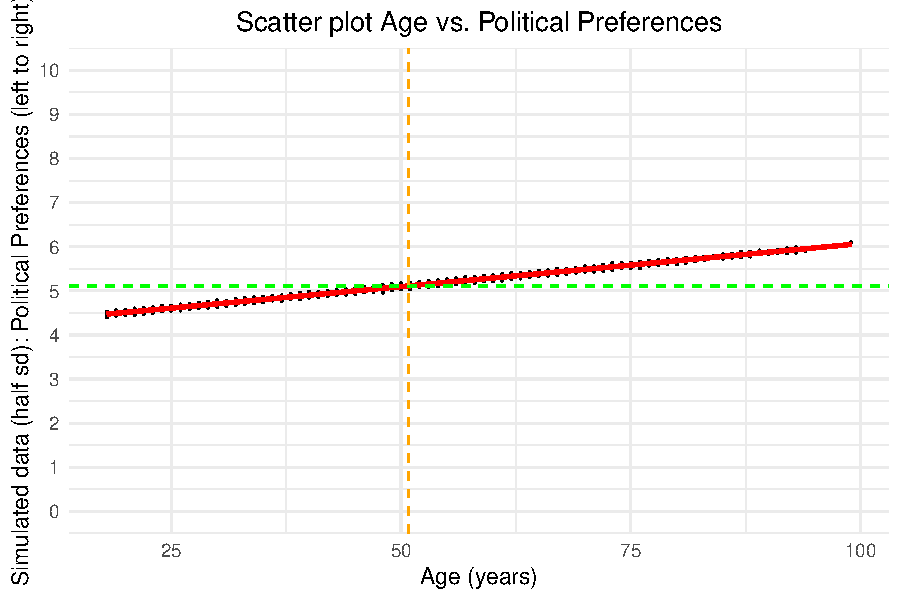
\includegraphics{_main_files/figure-latex/unnamed-chunk-85-1.pdf}

Report the new \(R^2\) here:

\begin{Shaded}
\begin{Highlighting}[]
\NormalTok{result }\OtherTok{\textless{}{-}} \FunctionTok{lm}\NormalTok{(Sim\_LeftToRight\_Det\_Stoch\_hsd }\SpecialCharTok{\textasciitilde{}}\NormalTok{ age, }\AttributeTok{data =}\NormalTok{ selects19)}
\NormalTok{rsq\_sd100 }\OtherTok{\textless{}{-}} \FunctionTok{summary}\NormalTok{(result)}\SpecialCharTok{$}\NormalTok{r.squared}
\FunctionTok{cat}\NormalTok{(}\StringTok{\textquotesingle{}The R2 is: \textquotesingle{}}\NormalTok{, rsq\_sd100)}
\end{Highlighting}
\end{Shaded}

\begin{verbatim}
## The R2 is:  0.9939772
\end{verbatim}

\begin{enumerate}
\def\labelenumi{\arabic{enumi}.}
\setcounter{enumi}{6}
\tightlist
\item
  Present in a table the \(R^2\) for each value of the standard deviation.
\end{enumerate}

\begin{Shaded}
\begin{Highlighting}[]
\NormalTok{table }\OtherTok{\textless{}{-}} \FunctionTok{data.frame}\NormalTok{(}
  \AttributeTok{SD =} \FunctionTok{c}\NormalTok{(}\DecValTok{1}\NormalTok{, }\FloatTok{0.1}\NormalTok{, }\FloatTok{0.01}\NormalTok{),}
  \AttributeTok{R2 =} \FunctionTok{c}\NormalTok{(rsq\_sd1, rsq\_sd10, rsq\_sd100)    }\CommentTok{\# Replace these with the actual R{-}squared values}
\NormalTok{)}

\FunctionTok{print}\NormalTok{(table)}
\end{Highlighting}
\end{Shaded}

\begin{verbatim}
##     SD        R2
## 1 1.00 0.0161515
## 2 0.10 0.6255030
## 3 0.01 0.9939772
\end{verbatim}

\begin{enumerate}
\def\labelenumi{\arabic{enumi}.}
\setcounter{enumi}{7}
\tightlist
\item
  Graph \(R^2\) agains the standard deviation fraction. Fit a linear regression line.
\end{enumerate}

\begin{Shaded}
\begin{Highlighting}[]
\FunctionTok{ggplot}\NormalTok{(table, }\FunctionTok{aes}\NormalTok{(}\AttributeTok{x =}\NormalTok{ SD, }\AttributeTok{y =}\NormalTok{ R2)) }\SpecialCharTok{+}
  \FunctionTok{geom\_point}\NormalTok{(}\AttributeTok{size =} \DecValTok{0}\NormalTok{) }\SpecialCharTok{+}
  \FunctionTok{geom\_smooth}\NormalTok{(}\AttributeTok{method =} \StringTok{"lm"}\NormalTok{, }\AttributeTok{formula =}\NormalTok{ y }\SpecialCharTok{\textasciitilde{}}\NormalTok{ x, }\AttributeTok{se =} \ConstantTok{FALSE}\NormalTok{, }\AttributeTok{color =} \StringTok{"green"}\NormalTok{)}\SpecialCharTok{+}
  \FunctionTok{theme\_minimal}\NormalTok{() }\SpecialCharTok{+}
  \FunctionTok{theme}\NormalTok{(}\AttributeTok{plot.title =} \FunctionTok{element\_text}\NormalTok{(}\AttributeTok{hjust =} \FloatTok{0.5}\NormalTok{)) }\SpecialCharTok{+}
  \FunctionTok{labs}\NormalTok{(}
    \AttributeTok{x =} \StringTok{"Fraction of standard deviation"}\NormalTok{,}
    \AttributeTok{y =} \StringTok{"R2"}\NormalTok{,}
    \AttributeTok{title =} \StringTok{"Relation between R2 and standard deviation of residuals"}
\NormalTok{  ) }
\end{Highlighting}
\end{Shaded}

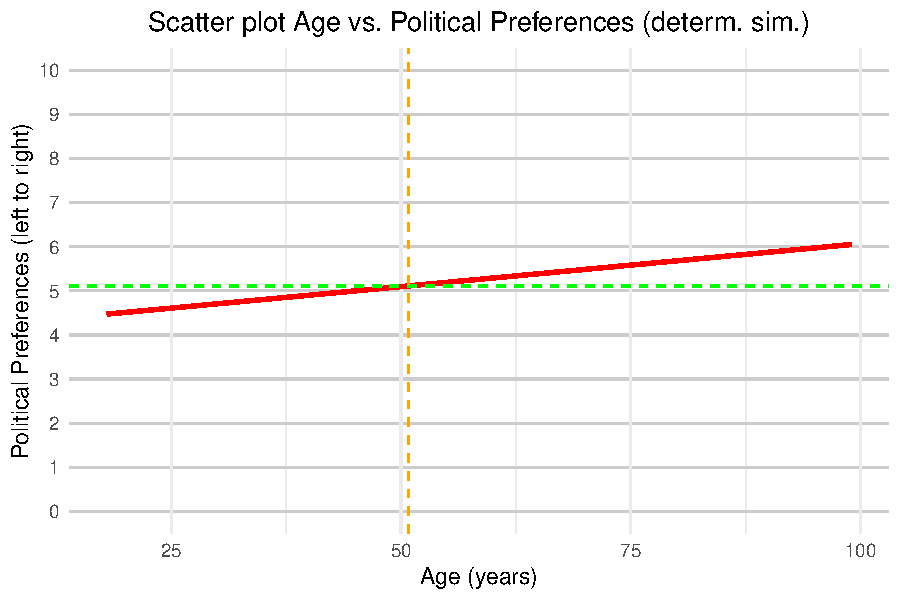
\includegraphics{_main_files/figure-latex/unnamed-chunk-88-1.pdf}
9. {[}Optional{]} Graph \(R^2\) against the standard deviation fraction. Fit a regression line with a polynomial of degree 2. The regression line fits the data better. Is the polynomial regression more informative than the linear regression? Why? What lesson does this graph give you in terms of the importance of understanding the theoretical relations between variables beyond what an empirical approach could suggest? What does it teach you regarding the tension between under- and over-fitting data?

\begin{Shaded}
\begin{Highlighting}[]
\FunctionTok{ggplot}\NormalTok{(table, }\FunctionTok{aes}\NormalTok{(}\AttributeTok{x =}\NormalTok{ SD, }\AttributeTok{y =}\NormalTok{ R2)) }\SpecialCharTok{+}
  \FunctionTok{geom\_point}\NormalTok{() }\SpecialCharTok{+}
  \FunctionTok{geom\_smooth}\NormalTok{(}\AttributeTok{method =} \StringTok{"lm"}\NormalTok{, }\AttributeTok{formula =}\NormalTok{ y }\SpecialCharTok{\textasciitilde{}} \FunctionTok{poly}\NormalTok{(x, }\DecValTok{2}\NormalTok{), }\AttributeTok{se =} \ConstantTok{FALSE}\NormalTok{, }\AttributeTok{color=}\StringTok{\textquotesingle{}green\textquotesingle{}}\NormalTok{) }\SpecialCharTok{+}
  \FunctionTok{theme\_minimal}\NormalTok{() }\SpecialCharTok{+}
  \FunctionTok{theme}\NormalTok{(}\AttributeTok{plot.title =} \FunctionTok{element\_text}\NormalTok{(}\AttributeTok{hjust =} \FloatTok{0.5}\NormalTok{)) }\SpecialCharTok{+}
  \FunctionTok{labs}\NormalTok{(}
    \AttributeTok{x =} \StringTok{"Fraction of standard deviation"}\NormalTok{,}
    \AttributeTok{y =} \StringTok{"R2"}\NormalTok{,}
    \AttributeTok{title =} \StringTok{"Relation between R2 and standard deviation of residuals"}
\NormalTok{  ) }
\end{Highlighting}
\end{Shaded}

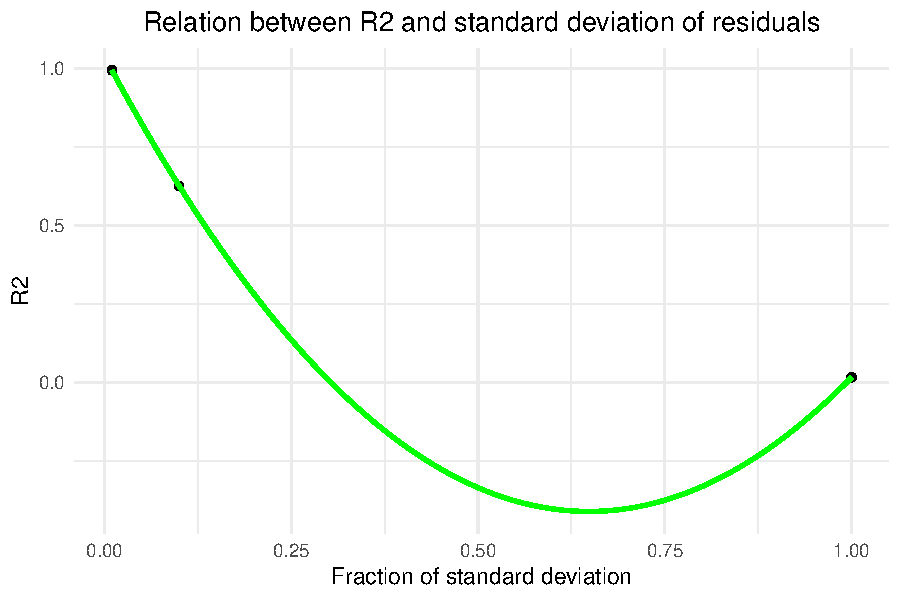
\includegraphics{_main_files/figure-latex/unnamed-chunk-89-1.pdf}
10. Print the parameters generated in the point 1. Generate the same predictions as in point 1 and 2 but this time multiply the slope's parameter by 5, while keeping the intercept unchanged. Call the resulting predictions \texttt{predicted\_LeftToRight\_AdjSlope} Generate a graph with the regression line for \texttt{predicted\_LeftToRight\_AdjSlope} vs \texttt{Age} and compare it with the graph \texttt{predicted\_LeftToRight} vs \texttt{Age} generated in point 1.

Print here

\begin{Shaded}
\begin{Highlighting}[]
\NormalTok{result }\OtherTok{\textless{}{-}} \FunctionTok{lm}\NormalTok{(LeftToRight }\SpecialCharTok{\textasciitilde{}}\NormalTok{ age, }\AttributeTok{data =}\NormalTok{ selects19)}
\CommentTok{\# summary(result)}
\NormalTok{coeffs }\OtherTok{\textless{}{-}} \FunctionTok{coef}\NormalTok{(result)}
\FunctionTok{cat}\NormalTok{(}\StringTok{\textquotesingle{}Intercept:\textquotesingle{}}\NormalTok{,}\FunctionTok{unname}\NormalTok{(coeffs[}\DecValTok{1}\NormalTok{]), }\StringTok{\textquotesingle{}}\SpecialCharTok{\textbackslash{}n\textbackslash{}n}\StringTok{Slope:\textquotesingle{}}\NormalTok{, }\FunctionTok{unname}\NormalTok{(coeffs[}\DecValTok{2}\NormalTok{]))}
\end{Highlighting}
\end{Shaded}

\begin{verbatim}
## Intercept: 4.122055 
## 
## Slope: 0.01948902
\end{verbatim}

Predict with the adjusted slope here.

\begin{Shaded}
\begin{Highlighting}[]
\NormalTok{selects19}\SpecialCharTok{$}\NormalTok{predicted\_LeftToRight\_AdjSlope }\OtherTok{\textless{}{-}} \FunctionTok{unname}\NormalTok{(coeffs[}\DecValTok{1}\NormalTok{])}\SpecialCharTok{+}\NormalTok{(}\FunctionTok{unname}\NormalTok{(coeffs[}\DecValTok{2}\NormalTok{])}\SpecialCharTok{*}\DecValTok{5}\NormalTok{)}\SpecialCharTok{*}\NormalTok{selects19}\SpecialCharTok{$}\NormalTok{age}
\end{Highlighting}
\end{Shaded}

Generate the graph here.

\begin{Shaded}
\begin{Highlighting}[]
\CommentTok{\#Means for Y and X}
\NormalTok{mean\_LeftRight }\OtherTok{\textless{}{-}} \FunctionTok{mean}\NormalTok{(selects19}\SpecialCharTok{$}\NormalTok{predicted\_LeftToRight\_AdjSlope, }\AttributeTok{na.rm =} \ConstantTok{TRUE}\NormalTok{)}
\NormalTok{mean\_age }\OtherTok{\textless{}{-}} \FunctionTok{mean}\NormalTok{(selects19}\SpecialCharTok{$}\NormalTok{age, }\AttributeTok{na.rm =} \ConstantTok{TRUE}\NormalTok{)}

\CommentTok{\# Create a scatter plot}
\FunctionTok{ggplot}\NormalTok{(selects19, }\FunctionTok{aes}\NormalTok{(}\AttributeTok{x =}\NormalTok{ age, }\AttributeTok{y =}\NormalTok{ predicted\_LeftToRight\_AdjSlope)) }\SpecialCharTok{+}
  \FunctionTok{geom\_smooth}\NormalTok{(}\AttributeTok{method =} \StringTok{"lm"}\NormalTok{, }\AttributeTok{formula =}\NormalTok{ y }\SpecialCharTok{\textasciitilde{}}\NormalTok{ x, }\AttributeTok{se =} \ConstantTok{FALSE}\NormalTok{, }\AttributeTok{color =} \StringTok{"red"}\NormalTok{) }\SpecialCharTok{+}  \CommentTok{\# Adding the regression line}
  \FunctionTok{geom\_hline}\NormalTok{(}\AttributeTok{yintercept =}\NormalTok{ mean\_LeftRight, }\AttributeTok{linetype =} \StringTok{"dashed"}\NormalTok{, }\AttributeTok{color =} \StringTok{"green"}\NormalTok{) }\SpecialCharTok{+}  \CommentTok{\# Horizontal line at the mean of y}
  \FunctionTok{geom\_vline}\NormalTok{(}\AttributeTok{xintercept =}\NormalTok{ mean\_age, }\AttributeTok{linetype =} \StringTok{"dashed"}\NormalTok{, }\AttributeTok{color =} \StringTok{"orange"}\NormalTok{) }\SpecialCharTok{+}  \CommentTok{\# Vertical line at the mean of x}
  \FunctionTok{theme\_minimal}\NormalTok{() }\SpecialCharTok{+}
  \FunctionTok{theme}\NormalTok{(}\AttributeTok{plot.title =} \FunctionTok{element\_text}\NormalTok{(}\AttributeTok{hjust =} \FloatTok{0.5}\NormalTok{)) }\SpecialCharTok{+}
  \FunctionTok{scale\_y\_continuous}\NormalTok{(}
    \AttributeTok{limits =} \FunctionTok{c}\NormalTok{(}\DecValTok{0}\NormalTok{, }\DecValTok{15}\NormalTok{),}
    \AttributeTok{breaks =} \FunctionTok{seq}\NormalTok{(}\DecValTok{0}\NormalTok{, }\DecValTok{20}\NormalTok{, }\AttributeTok{by =} \DecValTok{1}\NormalTok{)) }\SpecialCharTok{+}
  \FunctionTok{theme\_minimal}\NormalTok{() }\SpecialCharTok{+}
  \FunctionTok{theme}\NormalTok{(}
    \AttributeTok{plot.title =} \FunctionTok{element\_text}\NormalTok{(}\AttributeTok{hjust =} \FloatTok{0.5}\NormalTok{), }\CommentTok{\# Center the plot title}
    \AttributeTok{panel.grid.major.y =} \FunctionTok{element\_line}\NormalTok{(}\AttributeTok{color =} \StringTok{"grey80"}\NormalTok{, }\AttributeTok{size =} \FloatTok{0.5}\NormalTok{), }\CommentTok{\# Style for major Y grid lines}
    \AttributeTok{panel.grid.minor.y =} \FunctionTok{element\_blank}\NormalTok{() }\CommentTok{\# Remove minor Y grid lines}
\NormalTok{  ) }\SpecialCharTok{+}
  \FunctionTok{labs}\NormalTok{(}
    \AttributeTok{x =} \StringTok{"Age (years)"}\NormalTok{,}
    \AttributeTok{y =} \StringTok{"Political Preferences (left to right)"}\NormalTok{,}
    \AttributeTok{title =} \StringTok{"Scatter plot Age vs. Political Preferences (adj. slope)"}
\NormalTok{  )}
\end{Highlighting}
\end{Shaded}

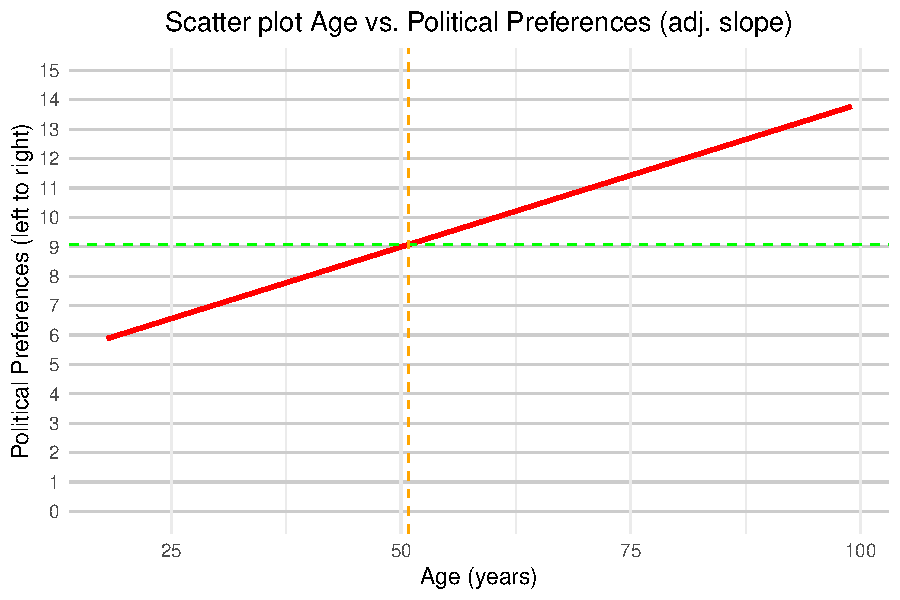
\includegraphics{_main_files/figure-latex/unnamed-chunk-92-1.pdf}
11. Add to the deterministic simulation the same stochastic component generated in point 2. Call that variable \texttt{predicted\_LeftToRight\_AdjSlope\_Stoch}. Generate the graph \texttt{predicted\_LeftToRight\_AdjSlope\_Stoch} vs \texttt{age} with a linear regression line. Generate the \(R^2\) and compare it to the one generated in point 4. Why is the new \(R^2\) higher than the one in point 4?

Report the simulation and the graph here.

\begin{Shaded}
\begin{Highlighting}[]
\NormalTok{selects19}\SpecialCharTok{$}\NormalTok{predicted\_LeftToRight\_AdjSlope\_Stoch }\OtherTok{\textless{}{-}}\NormalTok{ selects19}\SpecialCharTok{$}\NormalTok{predicted\_LeftToRight\_AdjSlope }\SpecialCharTok{+}\NormalTok{ selects19}\SpecialCharTok{$}\NormalTok{NormResiduals1}

\CommentTok{\#Means for Y and X}
\NormalTok{mean\_LeftRight }\OtherTok{\textless{}{-}} \FunctionTok{mean}\NormalTok{(selects19}\SpecialCharTok{$}\NormalTok{predicted\_LeftToRight\_AdjSlope\_Stoch, }\AttributeTok{na.rm =} \ConstantTok{TRUE}\NormalTok{)}
\NormalTok{mean\_age }\OtherTok{\textless{}{-}} \FunctionTok{mean}\NormalTok{(selects19}\SpecialCharTok{$}\NormalTok{age, }\AttributeTok{na.rm =} \ConstantTok{TRUE}\NormalTok{)}

\CommentTok{\# Create a scatter plot}
\FunctionTok{ggplot}\NormalTok{(selects19, }\FunctionTok{aes}\NormalTok{(}\AttributeTok{x =}\NormalTok{ age, }\AttributeTok{y =}\NormalTok{ predicted\_LeftToRight\_AdjSlope\_Stoch)) }\SpecialCharTok{+}
  \FunctionTok{geom\_point}\NormalTok{(}\AttributeTok{size =} \DecValTok{0}\NormalTok{) }\SpecialCharTok{+}
  \FunctionTok{geom\_smooth}\NormalTok{(}\AttributeTok{method =} \StringTok{"lm"}\NormalTok{, }\AttributeTok{formula =}\NormalTok{ y }\SpecialCharTok{\textasciitilde{}}\NormalTok{ x, }\AttributeTok{se =} \ConstantTok{FALSE}\NormalTok{, }\AttributeTok{color =} \StringTok{"red"}\NormalTok{) }\SpecialCharTok{+}  \CommentTok{\# Adding the regression line}
  \FunctionTok{geom\_hline}\NormalTok{(}\AttributeTok{yintercept =}\NormalTok{ mean\_LeftRight, }\AttributeTok{linetype =} \StringTok{"dashed"}\NormalTok{, }\AttributeTok{color =} \StringTok{"green"}\NormalTok{) }\SpecialCharTok{+}  \CommentTok{\# Horizontal line at the mean of y}
  \FunctionTok{geom\_vline}\NormalTok{(}\AttributeTok{xintercept =}\NormalTok{ mean\_age, }\AttributeTok{linetype =} \StringTok{"dashed"}\NormalTok{, }\AttributeTok{color =} \StringTok{"orange"}\NormalTok{) }\SpecialCharTok{+}  \CommentTok{\# Vertical line at the mean of x}
  \FunctionTok{scale\_y\_continuous}\NormalTok{(}
    \AttributeTok{limits =} \FunctionTok{c}\NormalTok{(}\DecValTok{0}\NormalTok{, }\DecValTok{20}\NormalTok{),}
    \AttributeTok{breaks =} \FunctionTok{seq}\NormalTok{(}\DecValTok{0}\NormalTok{, }\DecValTok{20}\NormalTok{, }\AttributeTok{by =} \DecValTok{1}\NormalTok{)) }\SpecialCharTok{+}
  \FunctionTok{theme\_minimal}\NormalTok{() }\SpecialCharTok{+}
  \FunctionTok{theme}\NormalTok{(}
    \AttributeTok{plot.title =} \FunctionTok{element\_text}\NormalTok{(}\AttributeTok{hjust =} \FloatTok{0.5}\NormalTok{), }\CommentTok{\# Center the plot title}
    \AttributeTok{panel.grid.major.y =} \FunctionTok{element\_line}\NormalTok{(}\AttributeTok{color =} \StringTok{"grey80"}\NormalTok{, }\AttributeTok{size =} \FloatTok{0.5}\NormalTok{), }\CommentTok{\# Style for major Y grid lines}
    \AttributeTok{panel.grid.minor.y =} \FunctionTok{element\_blank}\NormalTok{() }\CommentTok{\# Remove minor Y grid lines}
\NormalTok{  ) }\SpecialCharTok{+}
  \FunctionTok{labs}\NormalTok{(}
    \AttributeTok{x =} \StringTok{"Age (years)"}\NormalTok{,}
    \AttributeTok{y =} \StringTok{"Simulation: Political Preferences (left to right)"}\NormalTok{,}
    \AttributeTok{title =} \StringTok{"Scatter plot Age vs. Political Preferences }\SpecialCharTok{\textbackslash{}n}\StringTok{(determ.\& stoch. sim. with adjusted slope)"}
\NormalTok{  )}
\end{Highlighting}
\end{Shaded}

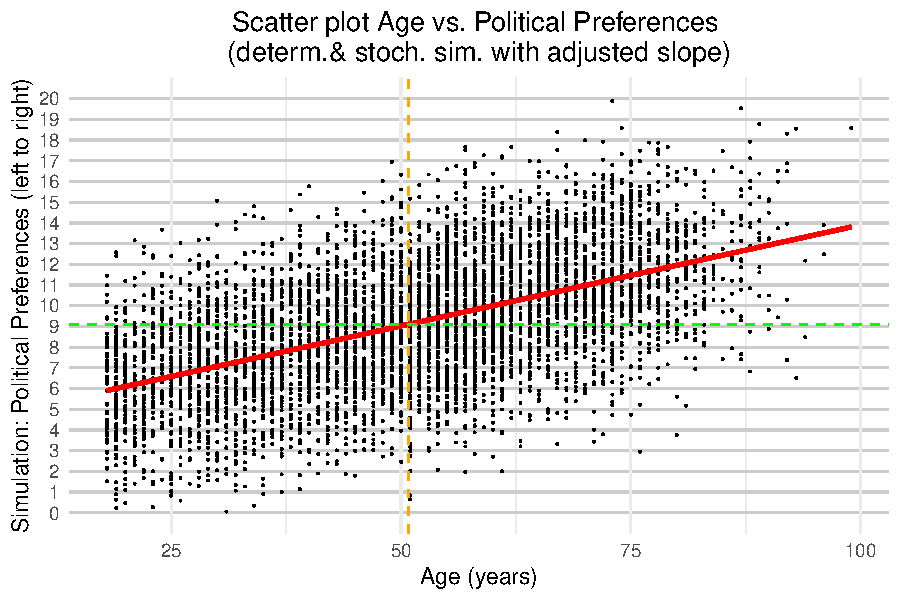
\includegraphics{_main_files/figure-latex/unnamed-chunk-93-1.pdf}

Report the new \(R^2\) here:

\begin{Shaded}
\begin{Highlighting}[]
\NormalTok{result }\OtherTok{\textless{}{-}} \FunctionTok{lm}\NormalTok{(predicted\_LeftToRight\_AdjSlope\_Stoch }\SpecialCharTok{\textasciitilde{}}\NormalTok{ age, }\AttributeTok{data =}\NormalTok{ selects19)}
\NormalTok{rsq\_sd1\_AdjSlope }\OtherTok{\textless{}{-}} \FunctionTok{summary}\NormalTok{(result)}\SpecialCharTok{$}\NormalTok{r.squared}
\FunctionTok{cat}\NormalTok{(}\StringTok{\textquotesingle{}The R2 is: \textquotesingle{}}\NormalTok{, rsq\_sd1\_AdjSlope)}
\end{Highlighting}
\end{Shaded}

\begin{verbatim}
## The R2 is:  0.2973214
\end{verbatim}

Report why is the new \(R^2\) higher than the one in point 4?

\begin{Shaded}
\begin{Highlighting}[]
\FunctionTok{print}\NormalTok{(}\StringTok{\textquotesingle{}The reason the R2 increased is that, while the distance from each observation to the regression line remained unchainged (i.e., the residual was kept unchanged), by increasing the slope of the generating process, the average distance between each observation and the average observation increased (i.e., Y}\SpecialCharTok{\textbackslash{}\textquotesingle{}}\StringTok{s variance increased). See the graph with the red and blue squares mentioned in point 5.\textquotesingle{}}\NormalTok{)}
\end{Highlighting}
\end{Shaded}

\begin{verbatim}
## [1] "The reason the R2 increased is that, while the distance from each observation to the regression line remained unchainged (i.e., the residual was kept unchanged), by increasing the slope of the generating process, the average distance between each observation and the average observation increased (i.e., Y's variance increased). See the graph with the red and blue squares mentioned in point 5."
\end{verbatim}

333333333333

\begin{enumerate}
\def\labelenumi{\arabic{enumi}.}
\setcounter{enumi}{11}
\tightlist
\item
  Print the parameters generated in the point 1. Generate the same predictions as in point 1 and 2 but this time increase in two units the \emph{intercept's} parameter (not the \emph{slope's} parameter as in the point 10), while keeping the slope unchanged. Call the resulting predictions \texttt{predicted\_LeftToRight\_AdjSlope} Generate a graph with the regression line for \texttt{predicted\_LeftToRight\_AdjSlope} vs \texttt{Age} and compare it with the graph \texttt{predicted\_LeftToRight} vs \texttt{Age} generated in point 1.
\end{enumerate}

Print here

\begin{Shaded}
\begin{Highlighting}[]
\NormalTok{result }\OtherTok{\textless{}{-}} \FunctionTok{lm}\NormalTok{(predicted\_LeftToRight\_AdjSlope\_Stoch }\SpecialCharTok{\textasciitilde{}}\NormalTok{ age, }\AttributeTok{data =}\NormalTok{ selects19)}
\CommentTok{\# summary(result)}
\NormalTok{coeffs12 }\OtherTok{\textless{}{-}} \FunctionTok{coef}\NormalTok{(result)}
\FunctionTok{cat}\NormalTok{(}\StringTok{\textquotesingle{}Intercept:\textquotesingle{}}\NormalTok{,}\FunctionTok{unname}\NormalTok{(coeffs12[}\DecValTok{1}\NormalTok{]), }\StringTok{\textquotesingle{}}\SpecialCharTok{\textbackslash{}n\textbackslash{}n}\StringTok{Slope:\textquotesingle{}}\NormalTok{, }\FunctionTok{unname}\NormalTok{(coeffs12[}\DecValTok{2}\NormalTok{]))}
\end{Highlighting}
\end{Shaded}

\begin{verbatim}
## Intercept: 4.071965 
## 
## Slope: 0.09874777
\end{verbatim}

Predict with the adjusted slope here.

\begin{Shaded}
\begin{Highlighting}[]
\NormalTok{selects19}\SpecialCharTok{$}\NormalTok{predicted\_LeftToRight\_AdjIntecept }\OtherTok{\textless{}{-}} \FunctionTok{unname}\NormalTok{(coeffs[}\DecValTok{1}\NormalTok{]}\SpecialCharTok{+}\DecValTok{2}\NormalTok{)}\SpecialCharTok{+}\NormalTok{(}\FunctionTok{unname}\NormalTok{(coeffs[}\DecValTok{2}\NormalTok{]))}\SpecialCharTok{*}\NormalTok{selects19}\SpecialCharTok{$}\NormalTok{age}
\end{Highlighting}
\end{Shaded}

Generate the graph here.

\begin{Shaded}
\begin{Highlighting}[]
\CommentTok{\#Means for Y and X}
\NormalTok{mean\_LeftRight }\OtherTok{\textless{}{-}} \FunctionTok{mean}\NormalTok{(selects19}\SpecialCharTok{$}\NormalTok{predicted\_LeftToRight\_AdjIntecept, }\AttributeTok{na.rm =} \ConstantTok{TRUE}\NormalTok{)}
\NormalTok{mean\_age }\OtherTok{\textless{}{-}} \FunctionTok{mean}\NormalTok{(selects19}\SpecialCharTok{$}\NormalTok{age, }\AttributeTok{na.rm =} \ConstantTok{TRUE}\NormalTok{)}

\CommentTok{\# Create a scatter plot}
\FunctionTok{ggplot}\NormalTok{(selects19, }\FunctionTok{aes}\NormalTok{(}\AttributeTok{x =}\NormalTok{ age, }\AttributeTok{y =}\NormalTok{ predicted\_LeftToRight\_AdjIntecept)) }\SpecialCharTok{+}
  \FunctionTok{geom\_smooth}\NormalTok{(}\AttributeTok{method =} \StringTok{"lm"}\NormalTok{, }\AttributeTok{formula =}\NormalTok{ y }\SpecialCharTok{\textasciitilde{}}\NormalTok{ x, }\AttributeTok{se =} \ConstantTok{FALSE}\NormalTok{, }\AttributeTok{color =} \StringTok{"red"}\NormalTok{) }\SpecialCharTok{+}  \CommentTok{\# Adding the regression line}
  \FunctionTok{geom\_hline}\NormalTok{(}\AttributeTok{yintercept =}\NormalTok{ mean\_LeftRight, }\AttributeTok{linetype =} \StringTok{"dashed"}\NormalTok{, }\AttributeTok{color =} \StringTok{"green"}\NormalTok{) }\SpecialCharTok{+}  \CommentTok{\# Horizontal line at the mean of y}
  \FunctionTok{geom\_vline}\NormalTok{(}\AttributeTok{xintercept =}\NormalTok{ mean\_age, }\AttributeTok{linetype =} \StringTok{"dashed"}\NormalTok{, }\AttributeTok{color =} \StringTok{"orange"}\NormalTok{) }\SpecialCharTok{+}  \CommentTok{\# Vertical line at the mean of x}
  \FunctionTok{theme\_minimal}\NormalTok{() }\SpecialCharTok{+}
  \FunctionTok{theme}\NormalTok{(}\AttributeTok{plot.title =} \FunctionTok{element\_text}\NormalTok{(}\AttributeTok{hjust =} \FloatTok{0.5}\NormalTok{)) }\SpecialCharTok{+}
  \FunctionTok{scale\_y\_continuous}\NormalTok{(}
    \AttributeTok{limits =} \FunctionTok{c}\NormalTok{(}\DecValTok{0}\NormalTok{, }\DecValTok{15}\NormalTok{),}
    \AttributeTok{breaks =} \FunctionTok{seq}\NormalTok{(}\DecValTok{0}\NormalTok{, }\DecValTok{20}\NormalTok{, }\AttributeTok{by =} \DecValTok{1}\NormalTok{)) }\SpecialCharTok{+}
  \FunctionTok{theme\_minimal}\NormalTok{() }\SpecialCharTok{+}
  \FunctionTok{theme}\NormalTok{(}
    \AttributeTok{plot.title =} \FunctionTok{element\_text}\NormalTok{(}\AttributeTok{hjust =} \FloatTok{0.5}\NormalTok{), }\CommentTok{\# Center the plot title}
    \AttributeTok{panel.grid.major.y =} \FunctionTok{element\_line}\NormalTok{(}\AttributeTok{color =} \StringTok{"grey80"}\NormalTok{, }\AttributeTok{size =} \FloatTok{0.5}\NormalTok{), }\CommentTok{\# Style for major Y grid lines}
    \AttributeTok{panel.grid.minor.y =} \FunctionTok{element\_blank}\NormalTok{() }\CommentTok{\# Remove minor Y grid lines}
\NormalTok{  ) }\SpecialCharTok{+}
  \FunctionTok{labs}\NormalTok{(}
    \AttributeTok{x =} \StringTok{"Age (years)"}\NormalTok{,}
    \AttributeTok{y =} \StringTok{"Political Preferences (left to right)"}\NormalTok{,}
    \AttributeTok{title =} \StringTok{"Scatter plot Age vs. Political Preferences (adj. slope)"}
\NormalTok{  )}
\end{Highlighting}
\end{Shaded}

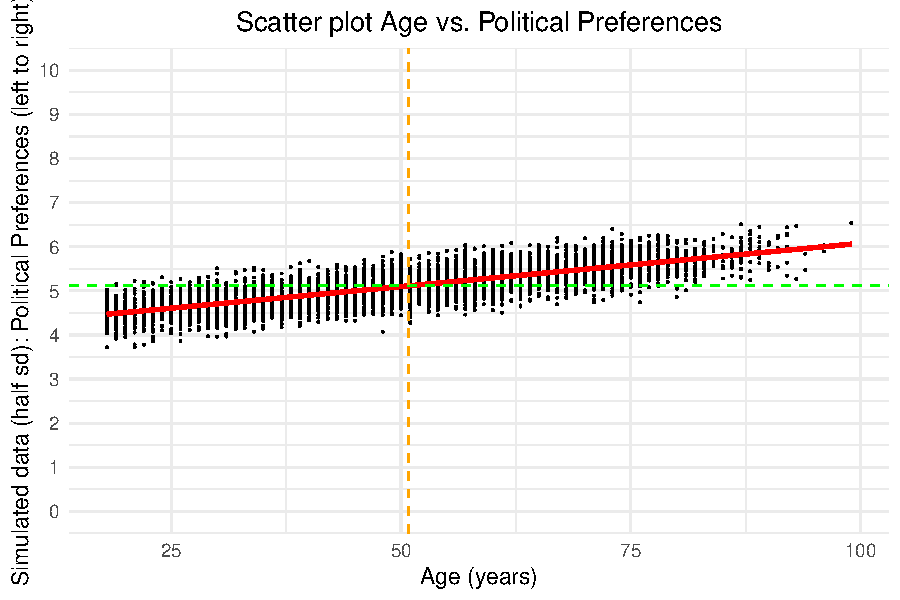
\includegraphics{_main_files/figure-latex/unnamed-chunk-98-1.pdf}
13. Add to the deterministic simulation the same stochastic component generated in point 2. Call that variable \texttt{predicted\_LeftToRight\_AdjIntercep\_Stoch}. Generate the graph \texttt{predicted\_LeftToRight\_AdjIntecept} vs \texttt{age} with a linear regression line. Generate the \(R^2\) and compare it to the one generated in point 4. Why is the new \(R^2\) higher than the one in point 4?

Report the simulation and the graph here.

\begin{Shaded}
\begin{Highlighting}[]
\NormalTok{selects19}\SpecialCharTok{$}\NormalTok{predicted\_LeftToRight\_AdjIntercept\_Stoch }\OtherTok{\textless{}{-}}\NormalTok{ selects19}\SpecialCharTok{$}\NormalTok{predicted\_LeftToRight\_AdjIntecept }\SpecialCharTok{+}\NormalTok{ selects19}\SpecialCharTok{$}\NormalTok{residual}

\CommentTok{\#Means for Y and X}
\NormalTok{mean\_LeftRight }\OtherTok{\textless{}{-}} \FunctionTok{mean}\NormalTok{(selects19}\SpecialCharTok{$}\NormalTok{predicted\_LeftToRight\_AdjIntercept\_Stoch, }\AttributeTok{na.rm =} \ConstantTok{TRUE}\NormalTok{)}
\NormalTok{mean\_age }\OtherTok{\textless{}{-}} \FunctionTok{mean}\NormalTok{(selects19}\SpecialCharTok{$}\NormalTok{age, }\AttributeTok{na.rm =} \ConstantTok{TRUE}\NormalTok{)}

\CommentTok{\# Create a scatter plot}
\FunctionTok{ggplot}\NormalTok{(selects19, }\FunctionTok{aes}\NormalTok{(}\AttributeTok{x =}\NormalTok{ age, }\AttributeTok{y =}\NormalTok{ predicted\_LeftToRight\_AdjIntercept\_Stoch)) }\SpecialCharTok{+}
  \FunctionTok{geom\_point}\NormalTok{(}\AttributeTok{size =} \DecValTok{0}\NormalTok{) }\SpecialCharTok{+}
  \FunctionTok{geom\_smooth}\NormalTok{(}\AttributeTok{method =} \StringTok{"lm"}\NormalTok{, }\AttributeTok{formula =}\NormalTok{ y }\SpecialCharTok{\textasciitilde{}}\NormalTok{ x, }\AttributeTok{se =} \ConstantTok{FALSE}\NormalTok{, }\AttributeTok{color =} \StringTok{"red"}\NormalTok{) }\SpecialCharTok{+}  \CommentTok{\# Adding the regression line}
  \FunctionTok{geom\_hline}\NormalTok{(}\AttributeTok{yintercept =}\NormalTok{ mean\_LeftRight, }\AttributeTok{linetype =} \StringTok{"dashed"}\NormalTok{, }\AttributeTok{color =} \StringTok{"green"}\NormalTok{) }\SpecialCharTok{+}  \CommentTok{\# Horizontal line at the mean of y}
  \FunctionTok{geom\_vline}\NormalTok{(}\AttributeTok{xintercept =}\NormalTok{ mean\_age, }\AttributeTok{linetype =} \StringTok{"dashed"}\NormalTok{, }\AttributeTok{color =} \StringTok{"orange"}\NormalTok{) }\SpecialCharTok{+}  \CommentTok{\# Vertical line at the mean of x}
  \FunctionTok{scale\_y\_continuous}\NormalTok{(}
    \AttributeTok{limits =} \FunctionTok{c}\NormalTok{(}\DecValTok{0}\NormalTok{, }\DecValTok{20}\NormalTok{),}
    \AttributeTok{breaks =} \FunctionTok{seq}\NormalTok{(}\DecValTok{0}\NormalTok{, }\DecValTok{20}\NormalTok{, }\AttributeTok{by =} \DecValTok{1}\NormalTok{)) }\SpecialCharTok{+}
  \FunctionTok{theme\_minimal}\NormalTok{() }\SpecialCharTok{+}
  \FunctionTok{theme}\NormalTok{(}
    \AttributeTok{plot.title =} \FunctionTok{element\_text}\NormalTok{(}\AttributeTok{hjust =} \FloatTok{0.5}\NormalTok{), }\CommentTok{\# Center the plot title}
    \AttributeTok{panel.grid.major.y =} \FunctionTok{element\_line}\NormalTok{(}\AttributeTok{color =} \StringTok{"grey80"}\NormalTok{, }\AttributeTok{size =} \FloatTok{0.5}\NormalTok{), }\CommentTok{\# Style for major Y grid lines}
    \AttributeTok{panel.grid.minor.y =} \FunctionTok{element\_blank}\NormalTok{() }\CommentTok{\# Remove minor Y grid lines}
\NormalTok{  ) }\SpecialCharTok{+}
  \FunctionTok{labs}\NormalTok{(}
    \AttributeTok{x =} \StringTok{"Age (years)"}\NormalTok{,}
    \AttributeTok{y =} \StringTok{"Simulation: Political Preferences (left to right)"}\NormalTok{,}
    \AttributeTok{title =} \StringTok{"Scatter plot Age vs. Political Preferences }\SpecialCharTok{\textbackslash{}n}\StringTok{(determ.\& stoch. sim. with adjusted intercept)"}
\NormalTok{  )}
\end{Highlighting}
\end{Shaded}

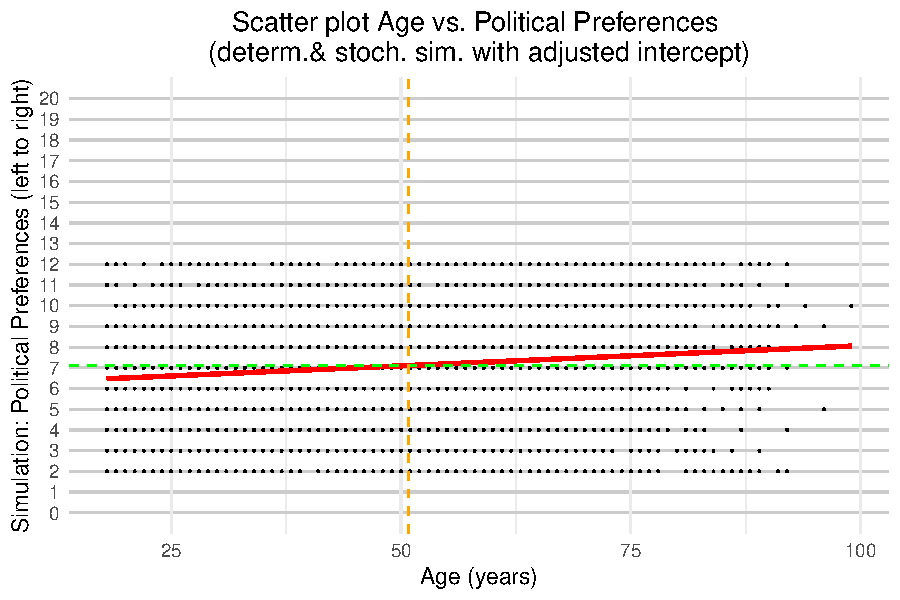
\includegraphics{_main_files/figure-latex/unnamed-chunk-99-1.pdf}
Regress the \texttt{predicted\_LeftToRight\_AdjIntercept\_Stoch} on \texttt{age}

\begin{Shaded}
\begin{Highlighting}[]
\NormalTok{result }\OtherTok{\textless{}{-}} \FunctionTok{lm}\NormalTok{(predicted\_LeftToRight\_AdjIntercept\_Stoch }\SpecialCharTok{\textasciitilde{}}\NormalTok{ age, }\AttributeTok{data =}\NormalTok{ selects19)}
\NormalTok{rsq\_sd1\_AdjIntercept }\OtherTok{\textless{}{-}} \FunctionTok{summary}\NormalTok{(result)}\SpecialCharTok{$}\NormalTok{r.squared}
\NormalTok{coeffs13 }\OtherTok{\textless{}{-}} \FunctionTok{coef}\NormalTok{(result)}
\FunctionTok{cat}\NormalTok{(}\StringTok{\textquotesingle{}Intercept:\textquotesingle{}}\NormalTok{,}\FunctionTok{unname}\NormalTok{(coeffs13[}\DecValTok{1}\NormalTok{]), }\StringTok{\textquotesingle{}}\SpecialCharTok{\textbackslash{}n\textbackslash{}n}\StringTok{Slope:\textquotesingle{}}\NormalTok{, }\FunctionTok{unname}\NormalTok{(coeffs13[}\DecValTok{2}\NormalTok{]))}
\end{Highlighting}
\end{Shaded}

\begin{verbatim}
## Intercept: 6.122055 
## 
## Slope: 0.01948902
\end{verbatim}

Report the \(R^2\) generated in points 2, 11, and 13 here:

\begin{Shaded}
\begin{Highlighting}[]
\NormalTok{tableSD1 }\OtherTok{\textless{}{-}} \FunctionTok{data.frame}\NormalTok{(}
  \AttributeTok{LookR2 =} \FunctionTok{c}\NormalTok{(}\StringTok{\textquotesingle{}Point 2\textquotesingle{}}\NormalTok{, }\StringTok{\textquotesingle{}Point 12\textquotesingle{}}\NormalTok{, }\StringTok{\textquotesingle{}Point 13\textquotesingle{}}\NormalTok{),}
  \AttributeTok{Model =} \FunctionTok{c}\NormalTok{(}\StringTok{\textquotesingle{}Unchanged\textquotesingle{}}\NormalTok{, }\StringTok{\textquotesingle{}P2 + (slope*5)\textquotesingle{}}\NormalTok{, }\StringTok{\textquotesingle{}P2+(intercept+2)\textquotesingle{}}\NormalTok{),}
  \AttributeTok{R2 =} \FunctionTok{c}\NormalTok{(rsq\_sd1, rsq\_sd1\_AdjSlope, rsq\_sd1\_AdjIntercept),    }
  \AttributeTok{LookParams =} \FunctionTok{c}\NormalTok{(}\StringTok{\textquotesingle{}Point 1\textquotesingle{}}\NormalTok{, }\StringTok{\textquotesingle{}Point 12\textquotesingle{}}\NormalTok{, }\StringTok{\textquotesingle{}Point 13\textquotesingle{}}\NormalTok{),}
  \AttributeTok{Intercept =} \FunctionTok{c}\NormalTok{(}\FunctionTok{unname}\NormalTok{(coeffs1[}\DecValTok{1}\NormalTok{]), }\FunctionTok{unname}\NormalTok{(coeffs12[}\DecValTok{1}\NormalTok{]), }\FunctionTok{unname}\NormalTok{(coeffs13[}\DecValTok{1}\NormalTok{])),    }
  \AttributeTok{Slope =} \FunctionTok{c}\NormalTok{(}\FunctionTok{unname}\NormalTok{(coeffs1[}\DecValTok{2}\NormalTok{]), }\FunctionTok{unname}\NormalTok{(coeffs12[}\DecValTok{2}\NormalTok{]), }\FunctionTok{unname}\NormalTok{(coeffs13[}\DecValTok{2}\NormalTok{]))}
\NormalTok{)}


\FunctionTok{print}\NormalTok{(tableSD1)}
\end{Highlighting}
\end{Shaded}

\begin{verbatim}
##     LookR2            Model        R2 LookParams Intercept      Slope
## 1  Point 2        Unchanged 0.0161515    Point 1  4.122055 0.01948902
## 2 Point 12   P2 + (slope*5) 0.2973214   Point 12  4.071965 0.09874777
## 3 Point 13 P2+(intercept+2) 0.0161515   Point 13  6.122055 0.01948902
\end{verbatim}

\begin{enumerate}
\def\labelenumi{\arabic{enumi}.}
\setcounter{enumi}{13}
\tightlist
\item
  Comparing the \(R^2\) and the parameters across the models of points 1, 2, and 3 answer the following questions:
\end{enumerate}

\begin{enumerate}
\def\labelenumi{\roman{enumi}.}
\tightlist
\item
  What effect does increasing the slope of the data generating process (while keeping the residuals and intercept unchanged) have on the \(R^2\)?
\end{enumerate}

\begin{Shaded}
\begin{Highlighting}[]
\FunctionTok{print}\NormalTok{(}\StringTok{\textquotesingle{}The R2 increases as seen in point 11\textquotesingle{}}\NormalTok{)}
\end{Highlighting}
\end{Shaded}

\begin{verbatim}
## [1] "The R2 increases as seen in point 11"
\end{verbatim}

\begin{enumerate}
\def\labelenumi{\roman{enumi}.}
\setcounter{enumi}{1}
\tightlist
\item
  What effect does increasing the intercept of the data generating process (while keeping the residuals and slope unchanged) have on the \(R^2\)?
\end{enumerate}

\begin{Shaded}
\begin{Highlighting}[]
\FunctionTok{print}\NormalTok{(}\StringTok{\textquotesingle{}The R2 stays unchanged as the distance from each observation to the regression line remained unchainged (i.e., the residual was kept unchanged) as well as the average distance between each observation and the average observation remained unchainged (i.e., Y}\SpecialCharTok{\textbackslash{}\textquotesingle{}}\StringTok{s variance was kept unchanged)\textquotesingle{}}\NormalTok{)}
\end{Highlighting}
\end{Shaded}

\begin{verbatim}
## [1] "The R2 stays unchanged as the distance from each observation to the regression line remained unchainged (i.e., the residual was kept unchanged) as well as the average distance between each observation and the average observation remained unchainged (i.e., Y's variance was kept unchanged)"
\end{verbatim}

\begin{enumerate}
\def\labelenumi{\roman{enumi}.}
\setcounter{enumi}{2}
\tightlist
\item
  What effect does increasing the slope of the data generating process (while keeping the residuals and intercept unchanged) have on the intercept and slope?
\end{enumerate}

\begin{Shaded}
\begin{Highlighting}[]
\FunctionTok{print}\NormalTok{(}\StringTok{\textquotesingle{}It increases the estimated slope and decreases the intercept.\textquotesingle{}}\NormalTok{)}
\end{Highlighting}
\end{Shaded}

\begin{verbatim}
## [1] "It increases the estimated slope and decreases the intercept."
\end{verbatim}

\begin{enumerate}
\def\labelenumi{\roman{enumi}.}
\setcounter{enumi}{3}
\tightlist
\item
  What effect does increasing the intercept of the data generating process (while keeping the residuals and slope unchanged) have on the intercept and slope?
\end{enumerate}

\begin{Shaded}
\begin{Highlighting}[]
\FunctionTok{print}\NormalTok{(}\StringTok{\textquotesingle{}It keeps the estimated slope unchanged and the estimated intercept is the same as before the adjustment but increases by the same value that the whole data generating process was modified.\textquotesingle{}}\NormalTok{)}
\end{Highlighting}
\end{Shaded}

\begin{verbatim}
## [1] "It keeps the estimated slope unchanged and the estimated intercept is the same as before the adjustment but increases by the same value that the whole data generating process was modified."
\end{verbatim}

\hypertarget{week-5}{%
\chapter{Week 5}\label{week-5}}

\hypertarget{exercise-1}{%
\section{Exercise}\label{exercise-1}}

\hypertarget{solution-2}{%
\section{Solution}\label{solution-2}}

\hypertarget{week-6}{%
\chapter{Week 6}\label{week-6}}

\hypertarget{exercise-2}{%
\section{Exercise}\label{exercise-2}}

\hypertarget{solution-3}{%
\section{Solution}\label{solution-3}}

\hypertarget{week-7}{%
\chapter{Week 7}\label{week-7}}

\hypertarget{exercise-3}{%
\section{Exercise}\label{exercise-3}}

\hypertarget{solution-4}{%
\section{Solution}\label{solution-4}}

\hypertarget{week-8-causality-iii-observational-data}{%
\chapter{Week 8: Causality III (Observational Data)}\label{week-8-causality-iii-observational-data}}

\hypertarget{aims-3}{%
\section{Aims}\label{aims-3}}

\begin{enumerate}
\def\labelenumi{\arabic{enumi}.}
\tightlist
\item
  Using simulated data to instantiate the logic behind, diff-in-diff and panel data (i.e., within, between, and twoway fixed effects) methods.
\item
  Using real data to estimate a causal effect using a two'way fixed effects model.
\end{enumerate}

\hypertarget{exercise-4}{%
\section{Exercise}\label{exercise-4}}

\hypertarget{simulated-data-2}{%
\subsection{Simulated data}\label{simulated-data-2}}

The following data is NOT real and is inspired by Ben Lambert's video on fixed effects (see \href{https://www.youtube.com/watch?v=1SchyQ77VFg}{here}). It's purpose is simply to illustrate the logic og the fixed effects models.

\begin{Shaded}
\begin{Highlighting}[]
\NormalTok{data }\OtherTok{\textless{}{-}} \FunctionTok{list}\NormalTok{(}
  \AttributeTok{City =} \FunctionTok{c}\NormalTok{(}\StringTok{\textquotesingle{}NYC\textquotesingle{}}\NormalTok{, }\StringTok{\textquotesingle{}NYC\textquotesingle{}}\NormalTok{, }\StringTok{\textquotesingle{}NYC\textquotesingle{}}\NormalTok{, }\StringTok{\textquotesingle{}Boston\textquotesingle{}}\NormalTok{, }\StringTok{\textquotesingle{}Boston\textquotesingle{}}\NormalTok{, }\StringTok{\textquotesingle{}Boston\textquotesingle{}}\NormalTok{, }\StringTok{\textquotesingle{}Amherst\textquotesingle{}}\NormalTok{, }\StringTok{\textquotesingle{}Amherst\textquotesingle{}}\NormalTok{, }\StringTok{\textquotesingle{}Amherst\textquotesingle{}}\NormalTok{),}
  \AttributeTok{Time =} \FunctionTok{c}\NormalTok{(}\DecValTok{1}\NormalTok{, }\DecValTok{2}\NormalTok{, }\DecValTok{3}\NormalTok{, }\DecValTok{1}\NormalTok{, }\DecValTok{2}\NormalTok{, }\DecValTok{3}\NormalTok{, }\DecValTok{1}\NormalTok{, }\DecValTok{2}\NormalTok{, }\DecValTok{3}\NormalTok{),}
  \AttributeTok{Unemployment =} \FunctionTok{c}\NormalTok{(}\DecValTok{2}\NormalTok{, }\DecValTok{3}\NormalTok{, }\DecValTok{3}\NormalTok{, }\DecValTok{4}\NormalTok{, }\DecValTok{5}\NormalTok{, }\DecValTok{5}\NormalTok{, }\DecValTok{6}\NormalTok{, }\DecValTok{7}\NormalTok{, }\DecValTok{8}\NormalTok{),}
  \AttributeTok{Crime =} \FunctionTok{c}\NormalTok{(}\DecValTok{5}\NormalTok{, }\DecValTok{6}\NormalTok{, }\DecValTok{9}\NormalTok{, }\DecValTok{3}\NormalTok{, }\DecValTok{4}\NormalTok{, }\DecValTok{7}\NormalTok{, }\DecValTok{1}\NormalTok{, }\DecValTok{2}\NormalTok{, }\DecValTok{3}\NormalTok{),}
  \AttributeTok{Treatment =} \FunctionTok{c}\NormalTok{(}\DecValTok{0}\NormalTok{, }\DecValTok{0}\NormalTok{, }\DecValTok{1}\NormalTok{, }\DecValTok{0}\NormalTok{, }\DecValTok{0}\NormalTok{, }\DecValTok{1}\NormalTok{, }\DecValTok{0}\NormalTok{, }\DecValTok{0}\NormalTok{, }\DecValTok{0}\NormalTok{)}
\NormalTok{)}

\NormalTok{df }\OtherTok{\textless{}{-}} \FunctionTok{data.frame}\NormalTok{(data)}

\CommentTok{\# Overall averages}
\NormalTok{df }\OtherTok{\textless{}{-}}\NormalTok{ df }\SpecialCharTok{\%\textgreater{}\%}
  \FunctionTok{mutate}\NormalTok{(}\AttributeTok{Y\_OverallAverage =} \FunctionTok{mean}\NormalTok{(Crime),}
         \AttributeTok{X\_OverallAverage =} \FunctionTok{mean}\NormalTok{(Unemployment))}

\CommentTok{\# Within averages         }
\NormalTok{df }\OtherTok{\textless{}{-}}\NormalTok{ df }\SpecialCharTok{\%\textgreater{}\%}
  \FunctionTok{group\_by}\NormalTok{(City) }\SpecialCharTok{\%\textgreater{}\%}
  \FunctionTok{mutate}\NormalTok{(}\AttributeTok{Y\_WithinAverage =} \FunctionTok{mean}\NormalTok{(Crime), }
         \AttributeTok{X\_WithinAverage =} \FunctionTok{mean}\NormalTok{(Unemployment))       }

\CommentTok{\# Between averages}
\NormalTok{df }\OtherTok{\textless{}{-}}\NormalTok{ df }\SpecialCharTok{\%\textgreater{}\%}
  \FunctionTok{group\_by}\NormalTok{(Time) }\SpecialCharTok{\%\textgreater{}\%}
  \FunctionTok{mutate}\NormalTok{(}\AttributeTok{Y\_BetweenAverage =} \FunctionTok{mean}\NormalTok{(Crime), }
         \AttributeTok{X\_BetweenAverage =} \FunctionTok{mean}\NormalTok{(Unemployment))}
         
\NormalTok{df}\OtherTok{\textless{}{-}}\NormalTok{ df }\SpecialCharTok{\%\textgreater{}\%}
  \FunctionTok{mutate}\NormalTok{( }\AttributeTok{Y\_demeaned\_within =}\NormalTok{ Crime}\SpecialCharTok{{-}}\NormalTok{Y\_WithinAverage,}
          \AttributeTok{Y\_demeaned\_between =}\NormalTok{ Crime}\SpecialCharTok{{-}}\NormalTok{Y\_BetweenAverage,}
          \AttributeTok{Y\_double\_demeaned =}\NormalTok{ Crime}\SpecialCharTok{{-}}\NormalTok{Y\_WithinAverage}\SpecialCharTok{{-}}\NormalTok{Y\_BetweenAverage}\SpecialCharTok{+}\NormalTok{Y\_OverallAverage,}
          \AttributeTok{X\_demeaned\_within =}\NormalTok{ Unemployment}\SpecialCharTok{{-}}\NormalTok{X\_WithinAverage,}
          \AttributeTok{X\_demeaned\_between =}\NormalTok{ Unemployment}\SpecialCharTok{{-}}\NormalTok{X\_BetweenAverage,}
          \AttributeTok{X\_double\_demeaned =}\NormalTok{ Unemployment}\SpecialCharTok{{-}}\NormalTok{X\_WithinAverage}\SpecialCharTok{{-}}\NormalTok{X\_BetweenAverage}\SpecialCharTok{+}\NormalTok{X\_OverallAverage}
\NormalTok{        )}
\end{Highlighting}
\end{Shaded}

First the basic graph

\begin{Shaded}
\begin{Highlighting}[]
\FunctionTok{ggplot}\NormalTok{(df, }\FunctionTok{aes}\NormalTok{(}\AttributeTok{x =}\NormalTok{ Unemployment, }\AttributeTok{y =}\NormalTok{ Crime)) }\SpecialCharTok{+}
  \FunctionTok{geom\_point}\NormalTok{(}\AttributeTok{size =} \DecValTok{5}\NormalTok{) }\SpecialCharTok{+}
  \FunctionTok{geom\_smooth}\NormalTok{(}\AttributeTok{method =} \StringTok{"lm"}\NormalTok{, }\AttributeTok{formula =}\NormalTok{ y }\SpecialCharTok{\textasciitilde{}}\NormalTok{ x, }\AttributeTok{se =} \ConstantTok{FALSE}\NormalTok{, }\AttributeTok{color =} \StringTok{"gray"}\NormalTok{) }\SpecialCharTok{+}  \CommentTok{\# Adding the regression line}

  \FunctionTok{scale\_y\_continuous}\NormalTok{(}
    \AttributeTok{limits =} \FunctionTok{c}\NormalTok{(}\DecValTok{0}\NormalTok{, }\DecValTok{10}\NormalTok{),}
    \AttributeTok{breaks =} \FunctionTok{seq}\NormalTok{(}\DecValTok{0}\NormalTok{, }\DecValTok{10}\NormalTok{, }\AttributeTok{by =} \DecValTok{1}\NormalTok{)) }\SpecialCharTok{+}
  \FunctionTok{theme\_minimal}\NormalTok{()}\SpecialCharTok{+}
  \FunctionTok{theme}\NormalTok{(}\AttributeTok{plot.title =} \FunctionTok{element\_text}\NormalTok{(}\AttributeTok{hjust =} \FloatTok{0.5}\NormalTok{)) }\SpecialCharTok{+}
  \FunctionTok{labs}\NormalTok{(}\AttributeTok{title =} \StringTok{"Unemployment vs Crime"}\NormalTok{,}
       \AttributeTok{x =} \StringTok{"Unemployment"}\NormalTok{,}
       \AttributeTok{y =} \StringTok{"Crime"}
\NormalTok{       )}
\end{Highlighting}
\end{Shaded}

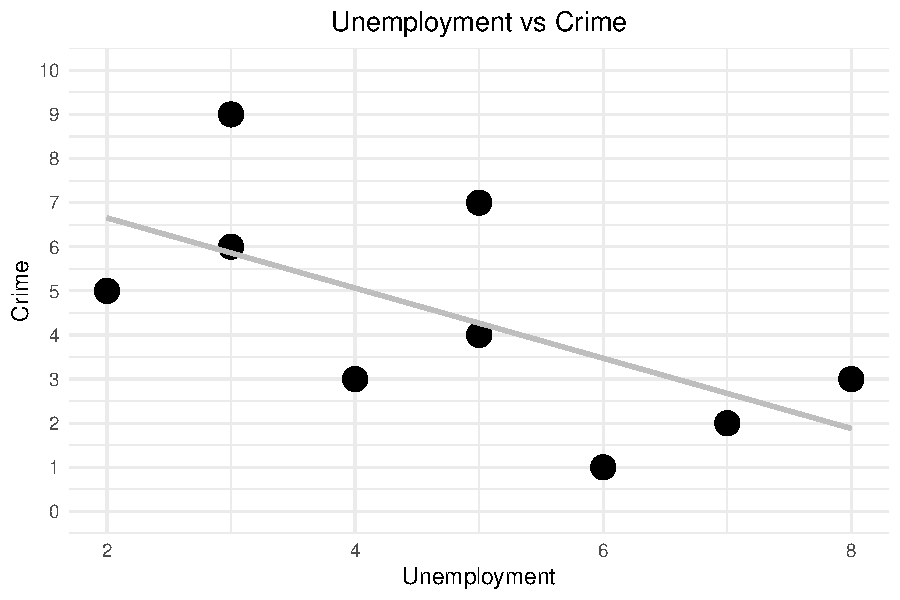
\includegraphics{_main_files/figure-latex/unnamed-chunk-113-1.pdf}

Now use shapes for distinguishing cities.

\begin{Shaded}
\begin{Highlighting}[]
\FunctionTok{ggplot}\NormalTok{(df, }\FunctionTok{aes}\NormalTok{(}\AttributeTok{x =}\NormalTok{ Unemployment, }\AttributeTok{y =}\NormalTok{ Crime)) }\SpecialCharTok{+}
  \FunctionTok{geom\_point}\NormalTok{(}\FunctionTok{aes}\NormalTok{(}\AttributeTok{shape =} \FunctionTok{factor}\NormalTok{(City)), }\AttributeTok{size =} \DecValTok{5}\NormalTok{) }\SpecialCharTok{+}  \CommentTok{\# Apply shape by City only to points}
  \FunctionTok{geom\_smooth}\NormalTok{(}\AttributeTok{method =} \StringTok{"lm"}\NormalTok{, }\AttributeTok{formula =}\NormalTok{ y }\SpecialCharTok{\textasciitilde{}}\NormalTok{ x, }\AttributeTok{se =} \ConstantTok{FALSE}\NormalTok{, }\AttributeTok{color =} \StringTok{"gray"}\NormalTok{) }\SpecialCharTok{+}  \CommentTok{\# Regression line for all data}
  \FunctionTok{scale\_y\_continuous}\NormalTok{(}
    \AttributeTok{limits =} \FunctionTok{c}\NormalTok{(}\DecValTok{0}\NormalTok{, }\DecValTok{10}\NormalTok{),}
    \AttributeTok{breaks =} \FunctionTok{seq}\NormalTok{(}\DecValTok{0}\NormalTok{, }\DecValTok{10}\NormalTok{, }\AttributeTok{by =} \DecValTok{1}\NormalTok{)) }\SpecialCharTok{+}
  \FunctionTok{theme\_minimal}\NormalTok{() }\SpecialCharTok{+}
  \FunctionTok{theme}\NormalTok{(}\AttributeTok{plot.title =} \FunctionTok{element\_text}\NormalTok{(}\AttributeTok{hjust =} \FloatTok{0.5}\NormalTok{)) }\SpecialCharTok{+}
  \FunctionTok{labs}\NormalTok{(}\AttributeTok{title =} \StringTok{"Unemployment vs Crime by City and Time"}\NormalTok{,}
       \AttributeTok{x =} \StringTok{"Unemployment"}\NormalTok{,}
       \AttributeTok{y =} \StringTok{"Crime"}\NormalTok{,}
       \AttributeTok{shape =} \StringTok{"City"}\NormalTok{)}
\end{Highlighting}
\end{Shaded}

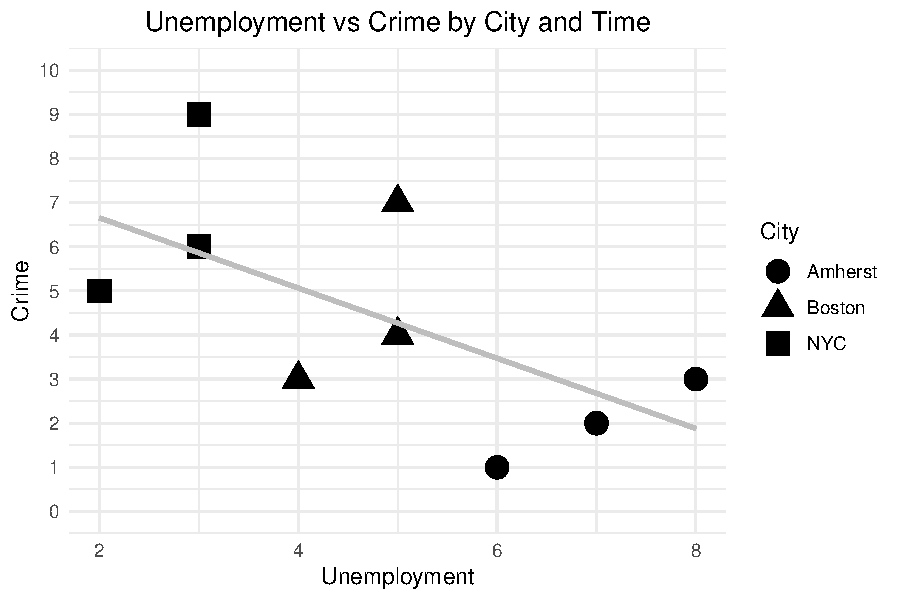
\includegraphics{_main_files/figure-latex/unnamed-chunk-114-1.pdf}

Now also use color for distinguishing also periods.

\begin{Shaded}
\begin{Highlighting}[]
\FunctionTok{ggplot}\NormalTok{(df, }\FunctionTok{aes}\NormalTok{(}\AttributeTok{x =}\NormalTok{ Unemployment, }\AttributeTok{y =}\NormalTok{ Crime)) }\SpecialCharTok{+}
  \FunctionTok{geom\_point}\NormalTok{(}\FunctionTok{aes}\NormalTok{(}\AttributeTok{shape =} \FunctionTok{factor}\NormalTok{(City), }\AttributeTok{color =} \FunctionTok{factor}\NormalTok{(Time)), }\AttributeTok{size =} \DecValTok{5}\NormalTok{) }\SpecialCharTok{+}  \CommentTok{\# Apply shape by City only to points}
  \FunctionTok{scale\_color\_manual}\NormalTok{(}\AttributeTok{values =} \FunctionTok{c}\NormalTok{(}\StringTok{"gold"}\NormalTok{, }\StringTok{"orange"}\NormalTok{, }\StringTok{"red"}\NormalTok{)) }\SpecialCharTok{+}
  \FunctionTok{geom\_smooth}\NormalTok{(}\AttributeTok{method =} \StringTok{"lm"}\NormalTok{, }\AttributeTok{formula =}\NormalTok{ y }\SpecialCharTok{\textasciitilde{}}\NormalTok{ x, }\AttributeTok{se =} \ConstantTok{FALSE}\NormalTok{, }\AttributeTok{color =} \StringTok{"gray"}\NormalTok{) }\SpecialCharTok{+}  \CommentTok{\# Regression line for all data}
  \FunctionTok{scale\_y\_continuous}\NormalTok{(}
    \AttributeTok{limits =} \FunctionTok{c}\NormalTok{(}\DecValTok{0}\NormalTok{, }\DecValTok{10}\NormalTok{),}
    \AttributeTok{breaks =} \FunctionTok{seq}\NormalTok{(}\DecValTok{0}\NormalTok{, }\DecValTok{10}\NormalTok{, }\AttributeTok{by =} \DecValTok{1}\NormalTok{)) }\SpecialCharTok{+}
  \FunctionTok{theme\_minimal}\NormalTok{() }\SpecialCharTok{+}
  \FunctionTok{theme}\NormalTok{(}\AttributeTok{plot.title =} \FunctionTok{element\_text}\NormalTok{(}\AttributeTok{hjust =} \FloatTok{0.5}\NormalTok{)) }\SpecialCharTok{+}
  \FunctionTok{labs}\NormalTok{(}\AttributeTok{title =} \StringTok{"Unemployment vs Crime by City and Time"}\NormalTok{,}
       \AttributeTok{x =} \StringTok{"Unemployment"}\NormalTok{,}
       \AttributeTok{y =} \StringTok{"Crime"}\NormalTok{,}
       \AttributeTok{color =} \StringTok{"Time"}\NormalTok{,}
       \AttributeTok{shape =} \StringTok{"City"}\NormalTok{)}
\end{Highlighting}
\end{Shaded}

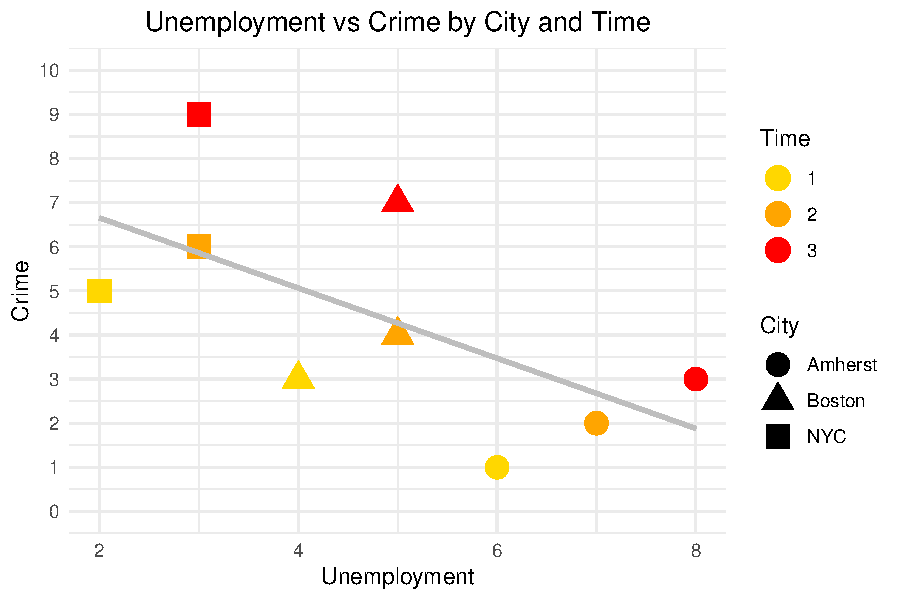
\includegraphics{_main_files/figure-latex/unnamed-chunk-115-1.pdf}

All previous regressions are counter intuitive, why?. Now restrict the regression to each city. What does this suggest regarding the ability of linear regression to capture relations between our variables of interest this scenario? Can we use a regression regardless of how we frame it? Is theory important for guiding how the regression is used? If so, in this case, how?

\begin{Shaded}
\begin{Highlighting}[]
\FunctionTok{ggplot}\NormalTok{(df, }\FunctionTok{aes}\NormalTok{(}\AttributeTok{x =}\NormalTok{ Unemployment, }\AttributeTok{y =}\NormalTok{ Crime, }\AttributeTok{color =} \FunctionTok{factor}\NormalTok{(Time), }\AttributeTok{shape =} \FunctionTok{factor}\NormalTok{(City))) }\SpecialCharTok{+}
  \FunctionTok{geom\_point}\NormalTok{(}\AttributeTok{size =} \DecValTok{5}\NormalTok{) }\SpecialCharTok{+}
  \FunctionTok{scale\_color\_manual}\NormalTok{(}\AttributeTok{values =} \FunctionTok{c}\NormalTok{(}\StringTok{"gold"}\NormalTok{, }\StringTok{"orange"}\NormalTok{, }\StringTok{"red"}\NormalTok{)) }\SpecialCharTok{+}
  \FunctionTok{geom\_smooth}\NormalTok{(}\AttributeTok{method =} \StringTok{"lm"}\NormalTok{, }\AttributeTok{formula =}\NormalTok{ y }\SpecialCharTok{\textasciitilde{}}\NormalTok{ x, }\AttributeTok{se =} \ConstantTok{FALSE}\NormalTok{, }\AttributeTok{color =} \StringTok{"gray"}\NormalTok{) }\SpecialCharTok{+}  \CommentTok{\# Adding the regression line}

  \FunctionTok{scale\_y\_continuous}\NormalTok{(}
  \AttributeTok{limits =} \FunctionTok{c}\NormalTok{(}\DecValTok{0}\NormalTok{, }\DecValTok{10}\NormalTok{),}
  \AttributeTok{breaks =} \FunctionTok{seq}\NormalTok{(}\DecValTok{0}\NormalTok{, }\DecValTok{10}\NormalTok{, }\AttributeTok{by =} \DecValTok{1}\NormalTok{)) }\SpecialCharTok{+}
  
  \FunctionTok{labs}\NormalTok{(}\AttributeTok{title =} \StringTok{"Unemployment vs Crime by City and Time"}\NormalTok{,}
       \AttributeTok{x =} \StringTok{"Unemployment"}\NormalTok{,}
       \AttributeTok{y =} \StringTok{"Crime"}\NormalTok{,}
       \AttributeTok{color =} \StringTok{"Time"}\NormalTok{,}
       \AttributeTok{shape =} \StringTok{"City"}\NormalTok{) }\SpecialCharTok{+}
  \FunctionTok{theme\_minimal}\NormalTok{()}
\end{Highlighting}
\end{Shaded}

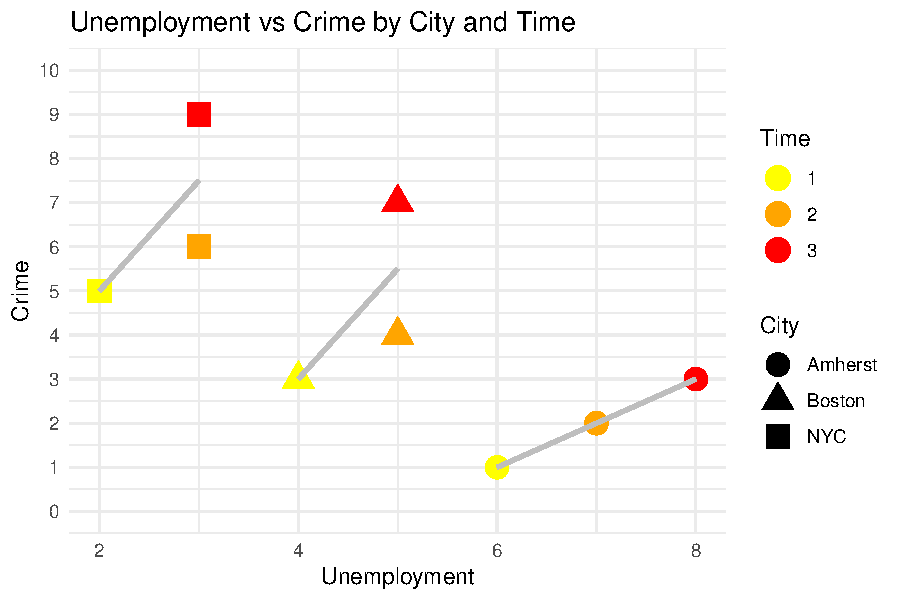
\includegraphics{_main_files/figure-latex/unnamed-chunk-116-1.pdf}

Now, having seen how regressions are theory dependent for defining how they are framed, let's see how fixed effects work.

Assume that the data generating process behind the relation between \texttt{unemployment} and \texttt{crime} is given by the following formula.

\[Y_{it}=\alpha_{i}+\beta_{t}+\gamma_{it}X_{it}+\epsilon_{it}\]
With \[t=1, ..., T\]
and
\[i=1, ..., N\]

Where \(Y_{it}\) is \texttt{crime} for city \(i\) at time \(t\), \(\alpha_{i}\) is a time invariant unobservable (or unobserved) factor influencing the levels of \texttt{crime} in city \(i\) (i.e., it's influence is constant across all periods). \(\beta_{t}\) is a city invariant unobservable (or unobserved) factor influencing the levels of \texttt{crime} at period \(t\) (i.e., it's influence is constant across all cities). \(\gamma_{it}\) is the marginal effect of \(X_{it}\), the \texttt{unemployment} level at city \(i\) in period \(t\). Finally, \(\epsilon_{it}\) is the residual for city \(i\) in period \(t\)

Thus, in order to get rid of the time invariant factor, we can implement the following transformation.

\(\bar{X}_{i.} = \frac{1}{T}*sum_{t=1}^{T} X_{it}.\)

{perhaps showing only the within case is enough? I'm considering to use \textbf{\href{https://economics.princeton.edu/wp-content/uploads/2021/08/two_way_mundlak-Wooldridge.pdf}{this}} paper, particularly page 8.}

Plus vertical line for within mean values.

\begin{Shaded}
\begin{Highlighting}[]
\NormalTok{X\_WithinAverage\_NYC }\OtherTok{=}\NormalTok{ df}\SpecialCharTok{$}\NormalTok{X\_WithinAverage[df}\SpecialCharTok{$}\NormalTok{City}\SpecialCharTok{==}\StringTok{\textquotesingle{}NYC\textquotesingle{}}\NormalTok{][}\DecValTok{1}\NormalTok{]}
\NormalTok{X\_WithinAverage\_Boston }\OtherTok{=}\NormalTok{ df}\SpecialCharTok{$}\NormalTok{X\_WithinAverage[df}\SpecialCharTok{$}\NormalTok{City}\SpecialCharTok{==}\StringTok{\textquotesingle{}Boston\textquotesingle{}}\NormalTok{][}\DecValTok{1}\NormalTok{]}
\NormalTok{X\_WithinAverage\_Amherst }\OtherTok{=}\NormalTok{ df}\SpecialCharTok{$}\NormalTok{X\_WithinAverage[df}\SpecialCharTok{$}\NormalTok{City}\SpecialCharTok{==}\StringTok{\textquotesingle{}Amherst\textquotesingle{}}\NormalTok{][}\DecValTok{1}\NormalTok{]}


\FunctionTok{ggplot}\NormalTok{(df, }\FunctionTok{aes}\NormalTok{(}\AttributeTok{x =}\NormalTok{ Unemployment, }\AttributeTok{y =}\NormalTok{ Crime, }\AttributeTok{color =} \FunctionTok{factor}\NormalTok{(Time), }\AttributeTok{shape =} \FunctionTok{factor}\NormalTok{(City))) }\SpecialCharTok{+}
  \FunctionTok{geom\_point}\NormalTok{(}\AttributeTok{size =} \DecValTok{5}\NormalTok{) }\SpecialCharTok{+}
  \FunctionTok{scale\_color\_manual}\NormalTok{(}\AttributeTok{values =} \FunctionTok{c}\NormalTok{(}\StringTok{"gold"}\NormalTok{, }\StringTok{"orange"}\NormalTok{, }\StringTok{"red"}\NormalTok{)) }\SpecialCharTok{+}
  \FunctionTok{geom\_smooth}\NormalTok{(}\AttributeTok{method =} \StringTok{"lm"}\NormalTok{, }\AttributeTok{formula =}\NormalTok{ y }\SpecialCharTok{\textasciitilde{}}\NormalTok{ x, }\AttributeTok{se =} \ConstantTok{FALSE}\NormalTok{, }\AttributeTok{color =} \StringTok{"gray"}\NormalTok{) }\SpecialCharTok{+}  \CommentTok{\# Adding the regression line}
  \FunctionTok{geom\_vline}\NormalTok{(}\AttributeTok{xintercept =}\NormalTok{ X\_WithinAverage\_NYC, }\AttributeTok{linetype =} \StringTok{"dashed"}\NormalTok{, }\AttributeTok{color =} \StringTok{"lightgray"}\NormalTok{) }\SpecialCharTok{+}  \CommentTok{\# Vertical line at the mean of}
  \FunctionTok{geom\_vline}\NormalTok{(}\AttributeTok{xintercept =}\NormalTok{ X\_WithinAverage\_Boston, }\AttributeTok{linetype =} \StringTok{"dashed"}\NormalTok{, }\AttributeTok{color =} \StringTok{"lightgray"}\NormalTok{) }\SpecialCharTok{+}  \CommentTok{\# Vertical line at the mean of}
  \FunctionTok{geom\_vline}\NormalTok{(}\AttributeTok{xintercept =}\NormalTok{ X\_WithinAverage\_Amherst, }\AttributeTok{linetype =} \StringTok{"dashed"}\NormalTok{, }\AttributeTok{color =} \StringTok{"lightgray"}\NormalTok{) }\SpecialCharTok{+}  \CommentTok{\# Vertical line at the mean of}
  \FunctionTok{scale\_y\_continuous}\NormalTok{(}
  \AttributeTok{limits =} \FunctionTok{c}\NormalTok{(}\DecValTok{0}\NormalTok{, }\DecValTok{10}\NormalTok{),}
  \AttributeTok{breaks =} \FunctionTok{seq}\NormalTok{(}\DecValTok{0}\NormalTok{, }\DecValTok{10}\NormalTok{, }\AttributeTok{by =} \DecValTok{1}\NormalTok{)) }\SpecialCharTok{+}
  
  \FunctionTok{labs}\NormalTok{(}\AttributeTok{title =} \StringTok{"Unemployment vs Crime by City and Time"}\NormalTok{,}
       \AttributeTok{x =} \StringTok{"Unemployment"}\NormalTok{,}
       \AttributeTok{y =} \StringTok{"Crime"}\NormalTok{,}
       \AttributeTok{color =} \StringTok{"Time"}\NormalTok{,}
       \AttributeTok{shape =} \StringTok{"City"}\NormalTok{) }\SpecialCharTok{+}
  \FunctionTok{theme\_minimal}\NormalTok{()}
\end{Highlighting}
\end{Shaded}

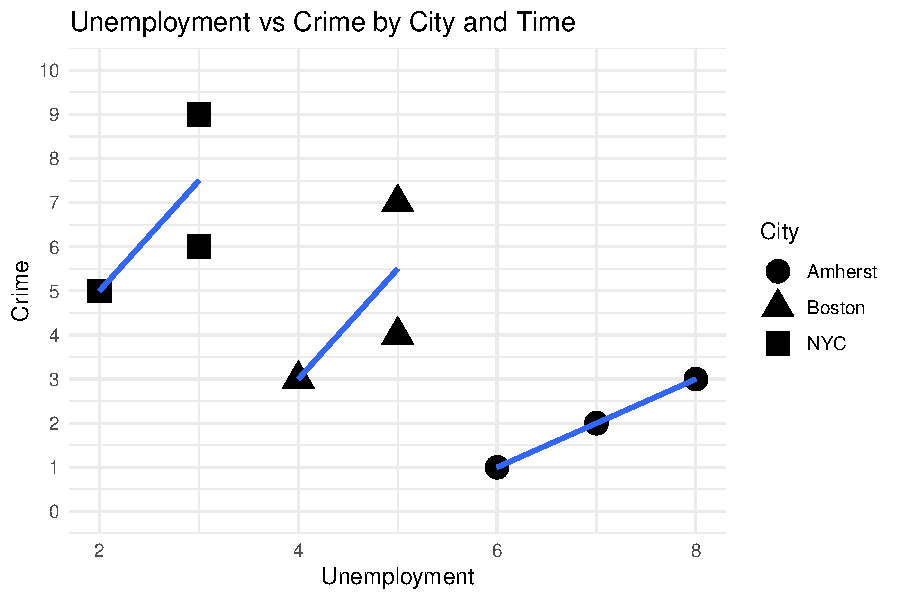
\includegraphics{_main_files/figure-latex/unnamed-chunk-117-1.pdf}

Demeaned within unemployment.

\begin{Shaded}
\begin{Highlighting}[]
\FunctionTok{ggplot}\NormalTok{(df, }\FunctionTok{aes}\NormalTok{(}\AttributeTok{x =}\NormalTok{ X\_demeaned\_within, }\AttributeTok{y =}\NormalTok{ Crime, }\AttributeTok{color =} \FunctionTok{factor}\NormalTok{(Time), }\AttributeTok{shape =} \FunctionTok{factor}\NormalTok{(City))) }\SpecialCharTok{+}
  \FunctionTok{geom\_point}\NormalTok{(}\AttributeTok{size =} \DecValTok{5}\NormalTok{) }\SpecialCharTok{+}
  \FunctionTok{scale\_color\_manual}\NormalTok{(}\AttributeTok{values =} \FunctionTok{c}\NormalTok{(}\StringTok{"gold"}\NormalTok{, }\StringTok{"orange"}\NormalTok{, }\StringTok{"red"}\NormalTok{)) }\SpecialCharTok{+}
  \FunctionTok{geom\_smooth}\NormalTok{(}\AttributeTok{method =} \StringTok{"lm"}\NormalTok{, }\AttributeTok{formula =}\NormalTok{ y }\SpecialCharTok{\textasciitilde{}}\NormalTok{ x, }\AttributeTok{se =} \ConstantTok{FALSE}\NormalTok{, }\AttributeTok{color =} \StringTok{"gray"}\NormalTok{) }\SpecialCharTok{+}  \CommentTok{\# Adding the regression line}
  \FunctionTok{scale\_y\_continuous}\NormalTok{(}
  \AttributeTok{limits =} \FunctionTok{c}\NormalTok{(}\DecValTok{0}\NormalTok{, }\DecValTok{10}\NormalTok{),}
  \AttributeTok{breaks =} \FunctionTok{seq}\NormalTok{(}\DecValTok{0}\NormalTok{, }\DecValTok{10}\NormalTok{, }\AttributeTok{by =} \DecValTok{1}\NormalTok{)) }\SpecialCharTok{+}
  
  \FunctionTok{labs}\NormalTok{(}\AttributeTok{title =} \StringTok{"Demeaned within unemployment vs Crime by City and Time"}\NormalTok{,}
       \AttributeTok{x =} \StringTok{"Demeaned unemployment"}\NormalTok{,}
       \AttributeTok{y =} \StringTok{"Crime"}\NormalTok{,}
       \AttributeTok{color =} \StringTok{"Time"}\NormalTok{,}
       \AttributeTok{shape =} \StringTok{"City"}\NormalTok{) }\SpecialCharTok{+}
  \FunctionTok{theme\_minimal}\NormalTok{()}
\end{Highlighting}
\end{Shaded}

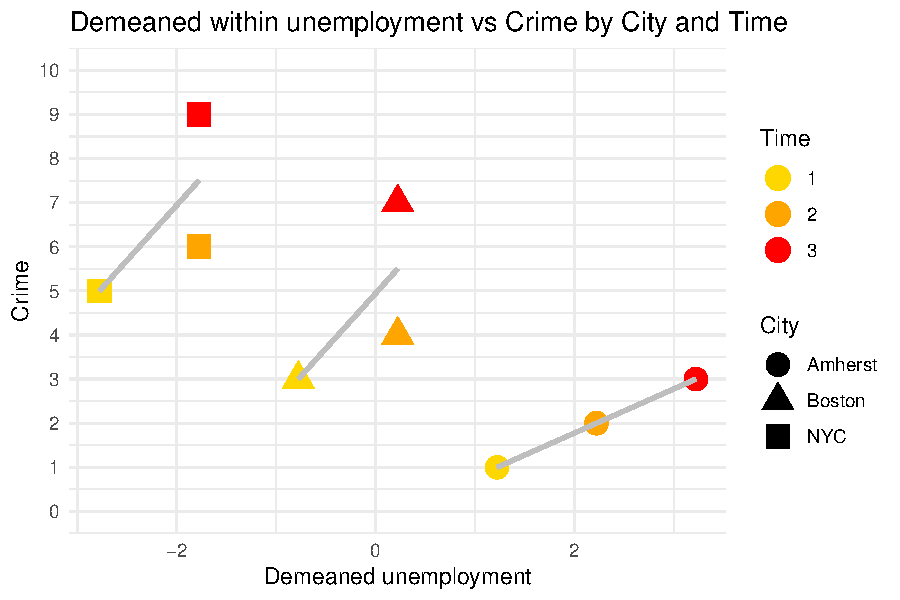
\includegraphics{_main_files/figure-latex/unnamed-chunk-118-1.pdf}

Also demeaned within crime.

\begin{Shaded}
\begin{Highlighting}[]
\FunctionTok{ggplot}\NormalTok{(df, }\FunctionTok{aes}\NormalTok{(}\AttributeTok{x =}\NormalTok{ X\_demeaned\_within, }\AttributeTok{y =}\NormalTok{ Y\_demeaned\_within)) }\SpecialCharTok{+}
  \FunctionTok{geom\_point}\NormalTok{(}\FunctionTok{aes}\NormalTok{(}\AttributeTok{shape =} \FunctionTok{factor}\NormalTok{(City), }\AttributeTok{color =} \FunctionTok{factor}\NormalTok{(Time)), }\AttributeTok{size =} \DecValTok{5}\NormalTok{) }\SpecialCharTok{+}
  \FunctionTok{scale\_color\_manual}\NormalTok{(}\AttributeTok{values =} \FunctionTok{c}\NormalTok{(}\StringTok{"gold"}\NormalTok{, }\StringTok{"orange"}\NormalTok{, }\StringTok{"red"}\NormalTok{)) }\SpecialCharTok{+}
  \FunctionTok{geom\_smooth}\NormalTok{(}\AttributeTok{method =} \StringTok{"lm"}\NormalTok{, }\AttributeTok{formula =}\NormalTok{ y }\SpecialCharTok{\textasciitilde{}}\NormalTok{ x, }\AttributeTok{se =} \ConstantTok{FALSE}\NormalTok{, }\AttributeTok{color =} \StringTok{"gray"}\NormalTok{) }\SpecialCharTok{+}  \CommentTok{\# Adding the regression line}

  \FunctionTok{labs}\NormalTok{(}\AttributeTok{title =} \StringTok{"Demeaned unemployment vs Demeaned crime by City and Time (within )"}\NormalTok{,}
       \AttributeTok{x =} \StringTok{"Demeaned unemployment"}\NormalTok{,}
       \AttributeTok{y =} \StringTok{"Demeaned crime"}\NormalTok{,}
       \AttributeTok{color =} \StringTok{"Time"}\NormalTok{,}
       \AttributeTok{shape =} \StringTok{"City"}\NormalTok{) }\SpecialCharTok{+}
  \FunctionTok{theme\_minimal}\NormalTok{()}
\end{Highlighting}
\end{Shaded}

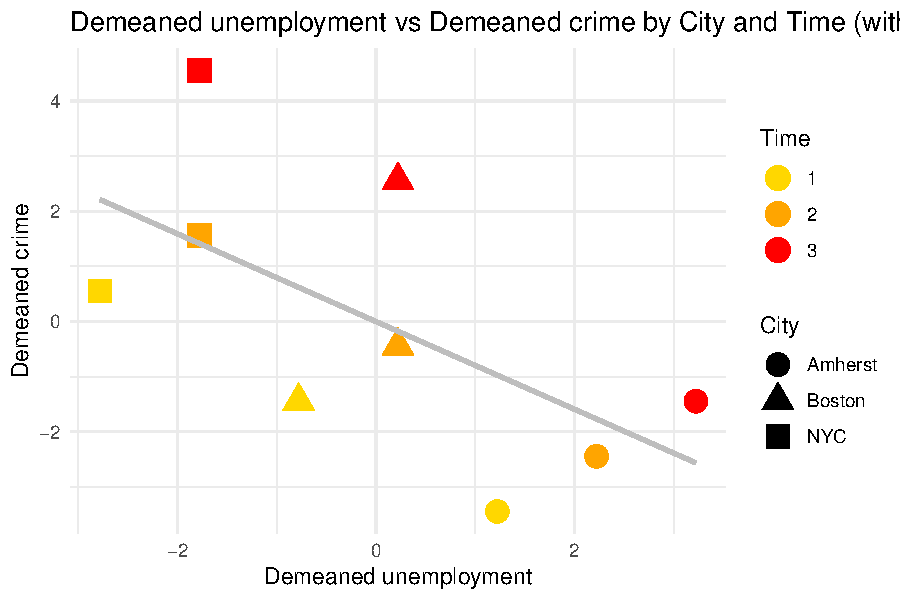
\includegraphics{_main_files/figure-latex/unnamed-chunk-119-1.pdf}

Unemployment over time with horizontal line for between mean values.

\begin{Shaded}
\begin{Highlighting}[]
\NormalTok{X\_BetweenAverage\_T1 }\OtherTok{=}\NormalTok{ df}\SpecialCharTok{$}\NormalTok{X\_BetweenAverage[df}\SpecialCharTok{$}\NormalTok{Time}\SpecialCharTok{==}\StringTok{\textquotesingle{}1\textquotesingle{}}\NormalTok{][}\DecValTok{1}\NormalTok{]}
\NormalTok{X\_BetweenAverage\_T2 }\OtherTok{=}\NormalTok{ df}\SpecialCharTok{$}\NormalTok{X\_BetweenAverage[df}\SpecialCharTok{$}\NormalTok{Time}\SpecialCharTok{==}\StringTok{\textquotesingle{}2\textquotesingle{}}\NormalTok{][}\DecValTok{1}\NormalTok{]}
\NormalTok{X\_BetweenAverage\_T3 }\OtherTok{=}\NormalTok{ df}\SpecialCharTok{$}\NormalTok{X\_BetweenAverage[df}\SpecialCharTok{$}\NormalTok{Time}\SpecialCharTok{==}\StringTok{\textquotesingle{}3\textquotesingle{}}\NormalTok{][}\DecValTok{1}\NormalTok{]}


\FunctionTok{ggplot}\NormalTok{(df, }\FunctionTok{aes}\NormalTok{(}\AttributeTok{x =}\NormalTok{ Time, }\AttributeTok{y =}\NormalTok{ Unemployment, }\AttributeTok{color =} \FunctionTok{factor}\NormalTok{(Time), }\AttributeTok{shape =} \FunctionTok{factor}\NormalTok{(City))) }\SpecialCharTok{+}
  \FunctionTok{geom\_point}\NormalTok{(}\AttributeTok{size =} \DecValTok{5}\NormalTok{) }\SpecialCharTok{+}
  \FunctionTok{scale\_color\_manual}\NormalTok{(}\AttributeTok{values =} \FunctionTok{c}\NormalTok{(}\StringTok{"gold"}\NormalTok{, }\StringTok{"orange"}\NormalTok{, }\StringTok{"red"}\NormalTok{)) }\SpecialCharTok{+}
  \FunctionTok{geom\_smooth}\NormalTok{(}\AttributeTok{method =} \StringTok{"lm"}\NormalTok{, }\AttributeTok{formula =}\NormalTok{ y }\SpecialCharTok{\textasciitilde{}}\NormalTok{ x, }\AttributeTok{se =} \ConstantTok{FALSE}\NormalTok{, }\AttributeTok{color =} \StringTok{"gray"}\NormalTok{) }\SpecialCharTok{+}  \CommentTok{\# Adding the regression line}
  \FunctionTok{geom\_hline}\NormalTok{(}\AttributeTok{yintercept =}\NormalTok{ X\_BetweenAverage\_T1, }\AttributeTok{linetype =} \StringTok{"dashed"}\NormalTok{, }\AttributeTok{color =} \StringTok{"gold"}\NormalTok{) }\SpecialCharTok{+}  \CommentTok{\# Vertical line at the mean of}
  \FunctionTok{geom\_hline}\NormalTok{(}\AttributeTok{yintercept =}\NormalTok{ X\_BetweenAverage\_T2, }\AttributeTok{linetype =} \StringTok{"dashed"}\NormalTok{, }\AttributeTok{color =} \StringTok{"orange"}\NormalTok{) }\SpecialCharTok{+}  \CommentTok{\# Vertical line at the mean of}
  \FunctionTok{geom\_hline}\NormalTok{(}\AttributeTok{yintercept =}\NormalTok{ X\_BetweenAverage\_T3, }\AttributeTok{linetype =} \StringTok{"dashed"}\NormalTok{, }\AttributeTok{color =} \StringTok{"red"}\NormalTok{) }\SpecialCharTok{+}  \CommentTok{\# Vertical line at the mean of}
  \FunctionTok{labs}\NormalTok{(}\AttributeTok{title =} \StringTok{"Time vs Unemployment by City and Time"}\NormalTok{,}
       \AttributeTok{x =} \StringTok{"Time"}\NormalTok{,}
       \AttributeTok{y =} \StringTok{"Unemployment"}\NormalTok{,}
       \AttributeTok{color =} \StringTok{"Time"}\NormalTok{,}
       \AttributeTok{shape =} \StringTok{"City"}\NormalTok{) }\SpecialCharTok{+}
  \FunctionTok{theme\_minimal}\NormalTok{()}
\end{Highlighting}
\end{Shaded}

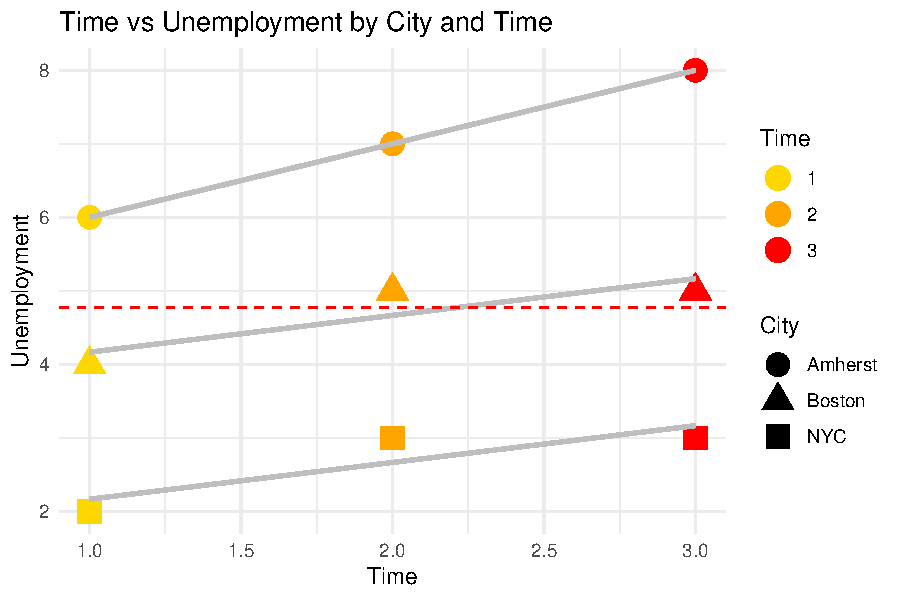
\includegraphics{_main_files/figure-latex/unnamed-chunk-120-1.pdf}

Crime over time with horizontal line for between mean values.

\begin{Shaded}
\begin{Highlighting}[]
\NormalTok{Y\_BetweenAverage\_T1 }\OtherTok{=}\NormalTok{ df}\SpecialCharTok{$}\NormalTok{Y\_BetweenAverage[df}\SpecialCharTok{$}\NormalTok{Time}\SpecialCharTok{==}\StringTok{\textquotesingle{}1\textquotesingle{}}\NormalTok{][}\DecValTok{1}\NormalTok{]}
\NormalTok{Y\_BetweenAverage\_T2 }\OtherTok{=}\NormalTok{ df}\SpecialCharTok{$}\NormalTok{Y\_BetweenAverage[df}\SpecialCharTok{$}\NormalTok{Time}\SpecialCharTok{==}\StringTok{\textquotesingle{}2\textquotesingle{}}\NormalTok{][}\DecValTok{1}\NormalTok{]}
\NormalTok{Y\_BetweenAverage\_T3 }\OtherTok{=}\NormalTok{ df}\SpecialCharTok{$}\NormalTok{Y\_BetweenAverage[df}\SpecialCharTok{$}\NormalTok{Time}\SpecialCharTok{==}\StringTok{\textquotesingle{}3\textquotesingle{}}\NormalTok{][}\DecValTok{1}\NormalTok{]}


\FunctionTok{ggplot}\NormalTok{(df, }\FunctionTok{aes}\NormalTok{(}\AttributeTok{x =}\NormalTok{ Time, }\AttributeTok{y =}\NormalTok{ Crime, }\AttributeTok{color =} \FunctionTok{factor}\NormalTok{(Time), }\AttributeTok{shape =} \FunctionTok{factor}\NormalTok{(City))) }\SpecialCharTok{+}
  \FunctionTok{geom\_point}\NormalTok{(}\AttributeTok{size =} \DecValTok{5}\NormalTok{) }\SpecialCharTok{+}
  \FunctionTok{scale\_color\_manual}\NormalTok{(}\AttributeTok{values =} \FunctionTok{c}\NormalTok{(}\StringTok{"gold"}\NormalTok{, }\StringTok{"orange"}\NormalTok{, }\StringTok{"red"}\NormalTok{)) }\SpecialCharTok{+}
  \FunctionTok{geom\_smooth}\NormalTok{(}\AttributeTok{method =} \StringTok{"lm"}\NormalTok{, }\AttributeTok{formula =}\NormalTok{ y }\SpecialCharTok{\textasciitilde{}}\NormalTok{ x, }\AttributeTok{se =} \ConstantTok{FALSE}\NormalTok{, }\AttributeTok{color =} \StringTok{"gray"}\NormalTok{) }\SpecialCharTok{+}  \CommentTok{\# Adding the regression line}
  \FunctionTok{geom\_hline}\NormalTok{(}\AttributeTok{yintercept =}\NormalTok{ Y\_BetweenAverage\_T1, }\AttributeTok{linetype =} \StringTok{"dotted"}\NormalTok{, }\AttributeTok{color =} \StringTok{"lightgray"}\NormalTok{) }\SpecialCharTok{+}  \CommentTok{\# Vertical line at the mean of}
  \FunctionTok{geom\_hline}\NormalTok{(}\AttributeTok{yintercept =}\NormalTok{ Y\_BetweenAverage\_T2, }\AttributeTok{linetype =} \StringTok{"twodash"}\NormalTok{, }\AttributeTok{color =} \StringTok{"lightgray"}\NormalTok{) }\SpecialCharTok{+}  \CommentTok{\# Vertical line at the mean of}
  \FunctionTok{geom\_hline}\NormalTok{(}\AttributeTok{yintercept =}\NormalTok{ Y\_BetweenAverage\_T3, }\AttributeTok{linetype =} \StringTok{"dashed"}\NormalTok{, }\AttributeTok{color =} \StringTok{"lightgray"}\NormalTok{) }\SpecialCharTok{+}  \CommentTok{\# Vertical line at the mean of}

  \FunctionTok{labs}\NormalTok{(}\AttributeTok{title =} \StringTok{"Time vs Crime by City and Time"}\NormalTok{,}
       \AttributeTok{x =} \StringTok{"Time"}\NormalTok{,}
       \AttributeTok{y =} \StringTok{"Crime"}\NormalTok{,}
       \AttributeTok{color =} \StringTok{"Time"}\NormalTok{,}
       \AttributeTok{shape =} \StringTok{"City"}\NormalTok{) }\SpecialCharTok{+}
  \FunctionTok{theme\_minimal}\NormalTok{()}
\end{Highlighting}
\end{Shaded}

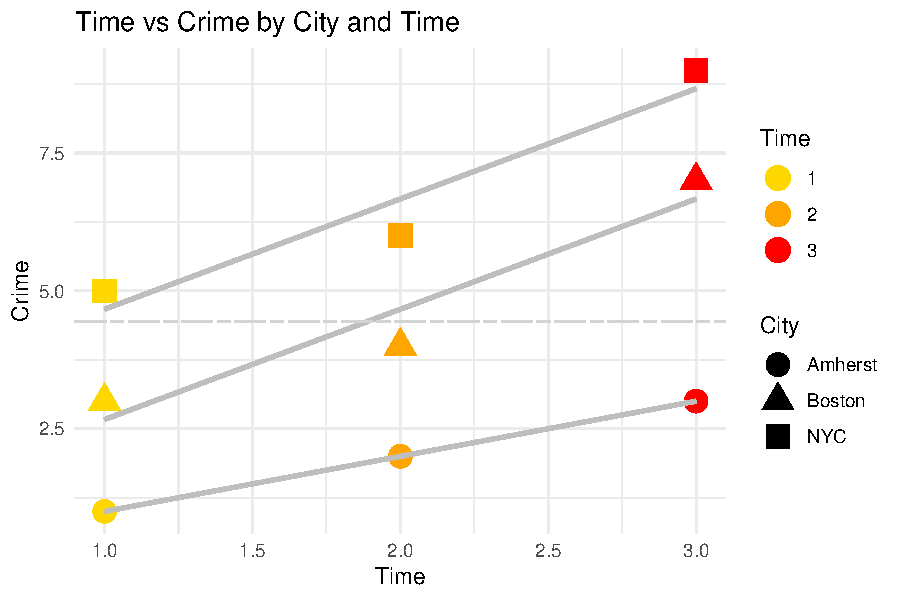
\includegraphics{_main_files/figure-latex/unnamed-chunk-121-1.pdf}

Demeaned unemployment over time with horizontal line for between mean values.

\begin{Shaded}
\begin{Highlighting}[]
\FunctionTok{ggplot}\NormalTok{(df, }\FunctionTok{aes}\NormalTok{(}\AttributeTok{x =}\NormalTok{ Time, }\AttributeTok{y =}\NormalTok{ X\_demeaned\_between, }\AttributeTok{color =} \FunctionTok{factor}\NormalTok{(Time), }\AttributeTok{shape =} \FunctionTok{factor}\NormalTok{(City))) }\SpecialCharTok{+}
  \FunctionTok{geom\_point}\NormalTok{(}\AttributeTok{size =} \DecValTok{5}\NormalTok{) }\SpecialCharTok{+}
  \FunctionTok{scale\_color\_manual}\NormalTok{(}\AttributeTok{values =} \FunctionTok{c}\NormalTok{(}\StringTok{"gold"}\NormalTok{, }\StringTok{"orange"}\NormalTok{, }\StringTok{"red"}\NormalTok{)) }\SpecialCharTok{+}
  \FunctionTok{geom\_smooth}\NormalTok{(}\AttributeTok{method =} \StringTok{"lm"}\NormalTok{, }\AttributeTok{formula =}\NormalTok{ y }\SpecialCharTok{\textasciitilde{}}\NormalTok{ x, }\AttributeTok{se =} \ConstantTok{FALSE}\NormalTok{, }\AttributeTok{color =} \StringTok{"gray"}\NormalTok{) }\SpecialCharTok{+}  \CommentTok{\# Adding the regression line}
  \FunctionTok{labs}\NormalTok{(}\AttributeTok{title =} \StringTok{"Time vs demeaned between unemployment by City and Time"}\NormalTok{,}
       \AttributeTok{x =} \StringTok{"Time"}\NormalTok{,}
       \AttributeTok{y =} \StringTok{"Demeaned unemployment"}\NormalTok{,}
       \AttributeTok{color =} \StringTok{"Time"}\NormalTok{,}
       \AttributeTok{shape =} \StringTok{"City"}\NormalTok{) }\SpecialCharTok{+}
  \FunctionTok{theme\_minimal}\NormalTok{()}
\end{Highlighting}
\end{Shaded}

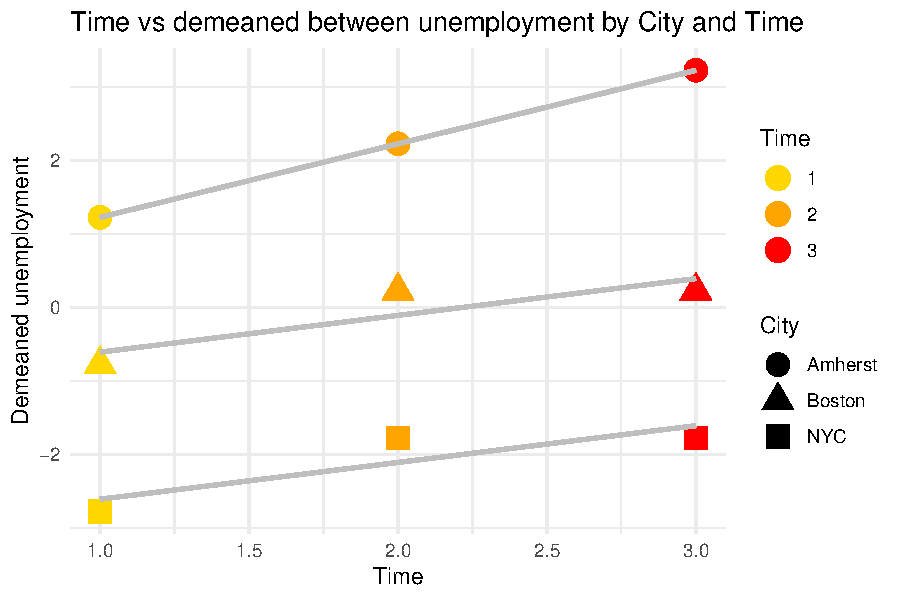
\includegraphics{_main_files/figure-latex/unnamed-chunk-122-1.pdf}

Demeaned crime over time with horizontal line for between mean values.

\begin{Shaded}
\begin{Highlighting}[]
\FunctionTok{ggplot}\NormalTok{(df, }\FunctionTok{aes}\NormalTok{(}\AttributeTok{x =}\NormalTok{ Time, }\AttributeTok{y =}\NormalTok{ Y\_demeaned\_between, }\AttributeTok{color =} \FunctionTok{factor}\NormalTok{(Time), }\AttributeTok{shape =} \FunctionTok{factor}\NormalTok{(City))) }\SpecialCharTok{+}
  \FunctionTok{geom\_point}\NormalTok{(}\AttributeTok{size =} \DecValTok{5}\NormalTok{) }\SpecialCharTok{+}
  \FunctionTok{scale\_color\_manual}\NormalTok{(}\AttributeTok{values =} \FunctionTok{c}\NormalTok{(}\StringTok{"gold"}\NormalTok{, }\StringTok{"orange"}\NormalTok{, }\StringTok{"red"}\NormalTok{)) }\SpecialCharTok{+}
  \FunctionTok{geom\_smooth}\NormalTok{(}\AttributeTok{method =} \StringTok{"lm"}\NormalTok{, }\AttributeTok{formula =}\NormalTok{ y }\SpecialCharTok{\textasciitilde{}}\NormalTok{ x, }\AttributeTok{se =} \ConstantTok{FALSE}\NormalTok{, }\AttributeTok{color =} \StringTok{"gray"}\NormalTok{) }\SpecialCharTok{+}  \CommentTok{\# Adding the regression line}
  \CommentTok{\# scale\_y\_continuous(}
  \CommentTok{\# limits = c(0, 10),}
  \CommentTok{\# breaks = seq(0, 10, by = 1)) +}
  
  \FunctionTok{labs}\NormalTok{(}\AttributeTok{title =} \StringTok{"Time vs demeaned between crime by City and Time"}\NormalTok{,}
       \AttributeTok{x =} \StringTok{"Time"}\NormalTok{,}
       \AttributeTok{y =} \StringTok{"Demeaned crime"}\NormalTok{,}
       \AttributeTok{color =} \StringTok{"Time"}\NormalTok{,}
       \AttributeTok{shape =} \StringTok{"City"}\NormalTok{) }\SpecialCharTok{+}
  \FunctionTok{theme\_minimal}\NormalTok{()}
\end{Highlighting}
\end{Shaded}

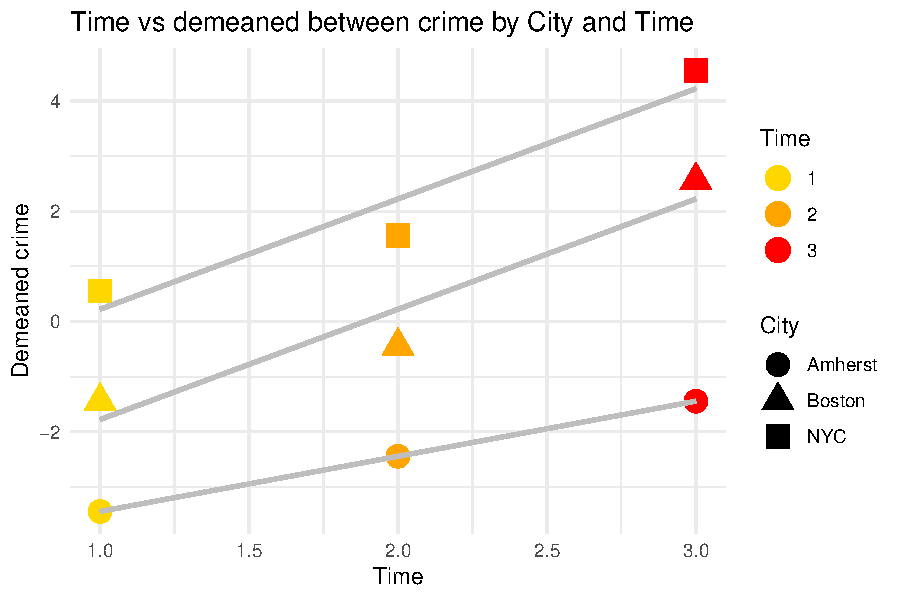
\includegraphics{_main_files/figure-latex/unnamed-chunk-123-1.pdf}

Demeaned crime over time with horizontal line for between mean values. \textbf{Very hard to interpret!}

\begin{Shaded}
\begin{Highlighting}[]
\FunctionTok{ggplot}\NormalTok{(df, }\FunctionTok{aes}\NormalTok{(}\AttributeTok{x =}\NormalTok{ X\_demeaned\_between, }\AttributeTok{y =}\NormalTok{ Y\_demeaned\_between)) }\SpecialCharTok{+}
  \FunctionTok{geom\_point}\NormalTok{(}\FunctionTok{aes}\NormalTok{(}\AttributeTok{shape =} \FunctionTok{factor}\NormalTok{(City), }\AttributeTok{color =} \FunctionTok{factor}\NormalTok{(Time)), }\AttributeTok{size =} \DecValTok{5}\NormalTok{) }\SpecialCharTok{+}  \CommentTok{\# Apply shape by City only to points}
  \FunctionTok{scale\_color\_manual}\NormalTok{(}\AttributeTok{values =} \FunctionTok{c}\NormalTok{(}\StringTok{"gold"}\NormalTok{, }\StringTok{"orange"}\NormalTok{, }\StringTok{"red"}\NormalTok{)) }\SpecialCharTok{+}
  \FunctionTok{geom\_smooth}\NormalTok{(}\AttributeTok{method =} \StringTok{"lm"}\NormalTok{, }\AttributeTok{formula =}\NormalTok{ y }\SpecialCharTok{\textasciitilde{}}\NormalTok{ x, }\AttributeTok{se =} \ConstantTok{FALSE}\NormalTok{, }\AttributeTok{color =} \StringTok{"gray"}\NormalTok{) }\SpecialCharTok{+}  \CommentTok{\# Adding the regression line}
  
  \FunctionTok{labs}\NormalTok{(}\AttributeTok{title =} \StringTok{"Demeaned unemployment vs demeaned crime by City and Time (between)"}\NormalTok{,}
       \AttributeTok{x =} \StringTok{"Demeaned unemployment"}\NormalTok{,}
       \AttributeTok{y =} \StringTok{"Demeaned crime"}\NormalTok{,}
       \AttributeTok{color =} \StringTok{"Time"}\NormalTok{,}
       \AttributeTok{shape =} \StringTok{"City"}\NormalTok{) }\SpecialCharTok{+}
  \FunctionTok{theme\_minimal}\NormalTok{()}
\end{Highlighting}
\end{Shaded}

\includegraphics{_main_files/figure-latex/unnamed-chunk-124-1.pdf}

{Missing!! all demeaned (i.e., twoway fixed effects)}

\hypertarget{real-data-2}{%
\subsection{Real data}\label{real-data-2}}

\begin{Shaded}
\begin{Highlighting}[]
\NormalTok{df1 }\OtherTok{\textless{}{-}}\NormalTok{ swissdd}\SpecialCharTok{::}\FunctionTok{get\_nationalvotes}\NormalTok{(}\AttributeTok{geolevel =} \StringTok{"national"}\NormalTok{, }\AttributeTok{from\_date=}\StringTok{"2000{-}03{-}12"}\NormalTok{, }\AttributeTok{to\_date =} \StringTok{"2015{-}06{-}14"}\NormalTok{)}

\NormalTok{df1}\OtherTok{\textless{}{-}}\NormalTok{ df1 }\SpecialCharTok{\%\textgreater{}\%}
  \FunctionTok{select}\NormalTok{(}\StringTok{"stimmbeteiligungInProzent"}\NormalTok{,}\StringTok{"votedate"}\NormalTok{)}
  
\NormalTok{df1 }\OtherTok{\textless{}{-}}\NormalTok{ dplyr}\SpecialCharTok{::}\FunctionTok{rename}\NormalTok{(df1, }\AttributeTok{Y\_National\_BetweenAverage =}\NormalTok{ stimmbeteiligungInProzent, }\AttributeTok{vote\_date =}\NormalTok{ votedate)}


\NormalTok{ballot\_days\_final }\OtherTok{\textless{}{-}} \FunctionTok{readRDS}\NormalTok{(}\StringTok{"/Users/fperil/Documents/0\_IPZ/2023\_2/Leemann{-}QuantMethods/QuantitativeMethods/QuantitativeMethods/Data/replication/data/ballot\_days\_final.rds"}\NormalTok{)  }

\NormalTok{ballot\_days\_final }\OtherTok{\textless{}{-}} \FunctionTok{inner\_join}\NormalTok{(ballot\_days\_final, df1, }\AttributeTok{by=}\StringTok{"vote\_date"}\NormalTok{)  }

\NormalTok{ballot\_days\_final }\OtherTok{\textless{}{-}}\NormalTok{ ballot\_days\_final }\SpecialCharTok{\%\textgreater{}\%}
  \FunctionTok{group\_by}\NormalTok{(muninr) }\SpecialCharTok{\%\textgreater{}\%}
  \FunctionTok{mutate}\NormalTok{(}\AttributeTok{Y\_municipal\_WithinAverage =} \FunctionTok{mean}\NormalTok{(turnout, }\AttributeTok{na.rm =} \ConstantTok{TRUE}\NormalTok{), }
         \AttributeTok{X\_municipal\_WithinAverage =} \FunctionTok{mean}\NormalTok{(postage, }\AttributeTok{na.rm =} \ConstantTok{TRUE}\NormalTok{))}


\NormalTok{ballot\_days\_final }\OtherTok{\textless{}{-}}\NormalTok{ ballot\_days\_final }\SpecialCharTok{\%\textgreater{}\%}
  \FunctionTok{mutate}\NormalTok{(}\AttributeTok{Y\_National\_OverallAverage =} \FunctionTok{mean}\NormalTok{(turnout, }\AttributeTok{na.rm =} \ConstantTok{TRUE}\NormalTok{),}
         \AttributeTok{X\_National\_OverallAverage =} \FunctionTok{mean}\NormalTok{(postage, }\AttributeTok{na.rm =} \ConstantTok{TRUE}\NormalTok{))}

\NormalTok{ballot\_days\_final }\OtherTok{\textless{}{-}}\NormalTok{ ballot\_days\_final }\SpecialCharTok{\%\textgreater{}\%}
  \FunctionTok{group\_by}\NormalTok{(vote\_date) }\SpecialCharTok{\%\textgreater{}\%}
  \FunctionTok{mutate}\NormalTok{(}\AttributeTok{X\_National\_BetweenAverage =} \FunctionTok{mean}\NormalTok{(postage, }\AttributeTok{na.rm =} \ConstantTok{TRUE}\NormalTok{))}
         

\NormalTok{ballot\_days\_final}\OtherTok{\textless{}{-}}\NormalTok{ ballot\_days\_final }\SpecialCharTok{\%\textgreater{}\%}
  \FunctionTok{mutate}\NormalTok{( }\AttributeTok{Y\_demeaned\_within =}\NormalTok{ turnout}\SpecialCharTok{{-}}\NormalTok{Y\_municipal\_WithinAverage,}
          \AttributeTok{Y\_demeaned\_between =}\NormalTok{ turnout}\SpecialCharTok{{-}}\NormalTok{Y\_National\_BetweenAverage,}
          \AttributeTok{Y\_double\_demeaned =}\NormalTok{ turnout}\SpecialCharTok{{-}}\NormalTok{Y\_municipal\_WithinAverage}\SpecialCharTok{{-}}\NormalTok{Y\_National\_BetweenAverage}\SpecialCharTok{+}\NormalTok{Y\_National\_OverallAverage,}
          \AttributeTok{X\_demeaned\_within =}\NormalTok{ postage}\SpecialCharTok{{-}}\NormalTok{X\_municipal\_WithinAverage,}
          \AttributeTok{X\_demeaned\_between =}\NormalTok{ postage}\SpecialCharTok{{-}}\NormalTok{X\_National\_BetweenAverage,}
          \AttributeTok{X\_double\_demeaned =}\NormalTok{ postage}\SpecialCharTok{{-}}\NormalTok{X\_municipal\_WithinAverage}\SpecialCharTok{{-}}\NormalTok{X\_National\_BetweenAverage}\SpecialCharTok{+}\NormalTok{X\_National\_OverallAverage}
\NormalTok{        )}
\end{Highlighting}
\end{Shaded}

Results: One way fixed effects: within

\begin{Shaded}
\begin{Highlighting}[]
\CommentTok{\# One way fixed effects: within}
\NormalTok{OW\_FE\_WI }\OtherTok{\textless{}{-}} \FunctionTok{lm}\NormalTok{(Y\_demeaned\_within }\SpecialCharTok{\textasciitilde{}}\NormalTok{ X\_demeaned\_within }\SpecialCharTok{{-}} \DecValTok{1}\NormalTok{, }\AttributeTok{data =}\NormalTok{ ballot\_days\_final)}
\FunctionTok{summary}\NormalTok{(OW\_FE\_WI)}
\end{Highlighting}
\end{Shaded}

\begin{verbatim}
## 
## Call:
## lm(formula = Y_demeaned_within ~ X_demeaned_within - 1, data = ballot_days_final)
## 
## Residuals:
##    Min     1Q Median     3Q    Max 
## -37.03  -6.53  -0.03   6.67  53.07 
## 
## Coefficients:
##                   Estimate Std. Error t value Pr(>|t|)    
## X_demeaned_within     1.46       0.15    9.73   <2e-16 ***
## ---
## Signif. codes:  0 '***' 0.001 '**' 0.01 '*' 0.05 '.' 0.1 ' ' 1
## 
## Residual standard error: 10.01 on 89319 degrees of freedom
##   (1210 observations deleted due to missingness)
## Multiple R-squared:  0.001059,   Adjusted R-squared:  0.001048 
## F-statistic: 94.67 on 1 and 89319 DF,  p-value: < 2.2e-16
\end{verbatim}

Results: One way fixed effects: between

\begin{Shaded}
\begin{Highlighting}[]
\CommentTok{\# One way fixed effects: between}
\NormalTok{OW\_FE\_BE }\OtherTok{\textless{}{-}} \FunctionTok{lm}\NormalTok{(Y\_demeaned\_between }\SpecialCharTok{\textasciitilde{}}\NormalTok{ X\_demeaned\_between }\SpecialCharTok{{-}} \DecValTok{1}\NormalTok{, }\AttributeTok{data =}\NormalTok{ ballot\_days\_final)}
\FunctionTok{summary}\NormalTok{(OW\_FE\_BE)}
\end{Highlighting}
\end{Shaded}

\begin{verbatim}
## 
## Call:
## lm(formula = Y_demeaned_between ~ X_demeaned_between - 1, data = ballot_days_final)
## 
## Residuals:
##     Min      1Q  Median      3Q     Max 
## -32.706  -6.728  -2.224   2.430  48.172 
## 
## Coefficients:
##                    Estimate Std. Error t value Pr(>|t|)    
## X_demeaned_between   1.3944     0.1132   12.32   <2e-16 ***
## ---
## Signif. codes:  0 '***' 0.001 '**' 0.01 '*' 0.05 '.' 0.1 ' ' 1
## 
## Residual standard error: 7.553 on 89319 degrees of freedom
##   (1210 observations deleted due to missingness)
## Multiple R-squared:  0.001696,   Adjusted R-squared:  0.001685 
## F-statistic: 151.8 on 1 and 89319 DF,  p-value: < 2.2e-16
\end{verbatim}

Results: Two way fixed effects: between

\begin{Shaded}
\begin{Highlighting}[]
\CommentTok{\# Two way fixed effects: between}
\NormalTok{TW\_FE }\OtherTok{\textless{}{-}} \FunctionTok{lm}\NormalTok{(Y\_double\_demeaned }\SpecialCharTok{\textasciitilde{}}\NormalTok{ X\_double\_demeaned }\SpecialCharTok{{-}} \DecValTok{1}\NormalTok{, }\AttributeTok{data =}\NormalTok{ ballot\_days\_final)}
\FunctionTok{summary}\NormalTok{(TW\_FE)}
\end{Highlighting}
\end{Shaded}

\begin{verbatim}
## 
## Call:
## lm(formula = Y_double_demeaned ~ X_double_demeaned - 1, data = ballot_days_final)
## 
## Residuals:
##     Min      1Q  Median      3Q     Max 
## -32.706  -6.728  -2.224   2.430  48.172 
## 
## Coefficients:
##                   Estimate Std. Error t value Pr(>|t|)    
## X_double_demeaned   1.3944     0.1132   12.32   <2e-16 ***
## ---
## Signif. codes:  0 '***' 0.001 '**' 0.01 '*' 0.05 '.' 0.1 ' ' 1
## 
## Residual standard error: 7.553 on 89319 degrees of freedom
##   (1210 observations deleted due to missingness)
## Multiple R-squared:  0.001696,   Adjusted R-squared:  0.001685 
## F-statistic: 151.8 on 1 and 89319 DF,  p-value: < 2.2e-16
\end{verbatim}

{Introduce here the estimation using \emph{plm} }

\hypertarget{week-9}{%
\chapter{Week 9}\label{week-9}}

\hypertarget{exercise-5}{%
\section{Exercise}\label{exercise-5}}

\hypertarget{solution-5}{%
\section{Solution}\label{solution-5}}

\hypertarget{week-10}{%
\chapter{Week 10}\label{week-10}}

\hypertarget{exercise-6}{%
\section{Exercise}\label{exercise-6}}

\hypertarget{solution-6}{%
\section{Solution}\label{solution-6}}

\hypertarget{week-11}{%
\chapter{Week 11}\label{week-11}}

\hypertarget{exercise-7}{%
\section{Exercise}\label{exercise-7}}

\hypertarget{solution-7}{%
\section{Solution}\label{solution-7}}

\hypertarget{week-12}{%
\chapter{Week 12}\label{week-12}}

\hypertarget{exercise-8}{%
\section{Exercise}\label{exercise-8}}

\hypertarget{solution-8}{%
\section{Solution}\label{solution-8}}

\hypertarget{week-13}{%
\chapter{Week 13}\label{week-13}}

\hypertarget{exercise-9}{%
\section{Exercise}\label{exercise-9}}

\hypertarget{solution-9}{%
\section{Solution}\label{solution-9}}

\hypertarget{week-14}{%
\chapter{Week 14}\label{week-14}}

\hypertarget{exercise-10}{%
\section{Exercise}\label{exercise-10}}

\hypertarget{solution-10}{%
\section{Solution}\label{solution-10}}

  \bibliography{book.bib,packages.bib}

\end{document}
